%% ====================================================================
%% GS-HCAL paper — NST (Nuclear Science and Techniques) wrapper
%% NST (Springer) currently accepts elsarticle format.
%% Uses elsarticle class (same as NIM A).
%% Compiled with: latexmk main_nst.tex
%% ====================================================================
\documentclass[preprint,12pt,times]{elsarticle}

%% --------------------------------------------------------------------
%% Packages
%% --------------------------------------------------------------------
\usepackage{amsmath,amssymb}
\usepackage{graphicx}
\usepackage{booktabs}
\usepackage{multirow}
\usepackage{subcaption}
\usepackage{xspace}
\usepackage{upgreek}
\usepackage[separate-uncertainty=true,multi-part-units=single]{siunitx}
\usepackage{float}
\usepackage{hyperref}
\usepackage{lineno}
\usepackage{xcolor}

%% Graphics path
\graphicspath{{figs/}}

%% --------------------------------------------------------------------
%% Unit macros
%% --------------------------------------------------------------------
\DeclareSIUnit\pe{p.e.}
\DeclareSIUnit\MIPunit{MIP}
\DeclareSIUnit\phMeV{ph/MeV}
\newcommand{\lambdaI}{\ensuremath{\lambda_{\mathrm{I}}}\xspace}
\newcommand{\peMIP}{\ensuremath{\text{p.e.}/\text{MIP}}\xspace}
\newcommand{\cellsize}{\ensuremath{40\times40\times10~\text{mm}^{3}}\xspace}
\newcommand{\sipmsize}{\ensuremath{3\times3~\text{mm}^{2}}\xspace}

%% Line numbers for review
\modulolinenumbers[5]
\journal{Nuclear Science and Techniques}

%% ====================================================================
\begin{document}
\begin{frontmatter}

\title{Baseline design and performance studies of the glass-scintillator
hadronic calorimeter for the CEPC reference detector}

%% --------------------------------------------------------------------
%% Authors — [PLACEHOLDER — replace with final author list]
%% --------------------------------------------------------------------
\author[scnu]{GS-HCAL Working Group}

\author[scnu]{Hengne~Li\corref{cor1}}
\ead{Hengne.Li@m.scnu.edu.cn}
\cortext[cor1]{Corresponding author}

\affiliation[scnu]{organization={South China Normal University},
  addressline={55 Zhongshan Avenue West},
  city={Guangzhou}, postcode={510631}, country={China}}

%% --------------------------------------------------------------------
%% Abstract
%% --------------------------------------------------------------------
\begin{abstract}
The Circular Electron-Positron Collider (CEPC) reference detector
requires a particle-flow-oriented hadronic calorimeter (HCAL) with
fine three-dimensional granularity, sufficient depth for hadronic
containment, and adequate energy resolution for neutral hadrons.
The Glass-Scintillator HCAL (GS-HCAL) is adopted as the baseline HCAL
of the CEPC reference detector: it employs high-density gadolinium
fluoro-oxide (GFO) glass-scintillator cells of \cellsize, each read
out by a \sipmsize silicon photomultiplier (SiPM), arranged in a
barrel and two endcaps totalling approximately 5.22~million channels
with a total depth of $6\,\lambdaI$ and a sampling fraction of
approximately~30\%.
Experimental characterisation shows a GFO light yield exceeding
\SI{1000}{\phMeV}, a light attenuation length of ${\sim}\SI{6}{cm}$
adequate for the baseline cell geometry, a radiation tolerance
retaining more than 70\% of the initial light yield at \SI{100}{Gy},
and single-cell measurements with a $^{137}$Cs source, cosmic-ray
muons ($63.6\pm0.5$~\peMIP), and \SI{5}{GeV} electrons at KEK
($157.6\pm2.9$~\peMIP).
Full Geant4 digitisation-based simulation of the baseline geometry
predicts a single-hadron energy resolution of
$\sigma_{E}/E = 29.8\%/\sqrt{E}\oplus6.5\%$, an energy non-linearity
within 2\%, and an $H\to gg$ boson mass resolution of 3.88\%, within
the CEPC target of 3--4\%.
Prototype beam-test validation is ongoing; the present study
establishes the technical and performance basis of the baseline
design, while detector-level closure of the remaining items is the
objective of the prototype programme.
\end{abstract}

\begin{keyword}
glass scintillator \sep
hadronic calorimeter \sep
CEPC \sep
silicon photomultiplier \sep
particle-flow algorithm \sep
gadolinium fluoro-oxide \sep
energy resolution \sep
highly granular calorimeter
\end{keyword}

\end{frontmatter}

\linenumbers

%% ====================================================================
%% GS-HCAL paper — shared body text
%% Baseline detector-technology paper for the CEPC reference detector
%% ====================================================================

%% ====================================================================
\section{Introduction}
\label{sec:intro}
%% ====================================================================

The Circular Electron-Positron Collider
(CEPC)~\cite{CEPCStudyGroup:2018ghi} will operate as a Higgs factory at
$\sqrt{s}=240$~GeV and as a high-luminosity $Z$-pole machine at
$\sqrt{s}=91.2$~GeV.
Within the Particle-Flow Algorithm
(PFA)~\cite{Thomson:2009rp,Brient:2004yq,Ruan:2013rkk} paradigm, the
Hadronic Calorimeter (HCAL) is responsible for the precise spatial
reconstruction and energy measurement of neutral hadrons, which carry
approximately 10\% of the jet energy and leave no tracks in the central
tracker.
The target boson mass resolution (BMR) of
3--4\%~\cite{CEPCStudyGroup:2018ghi} for $W$/$Z$/Higgs dijet final
states directly depends on the HCAL performance.
These requirements are satisfied only when the HCAL simultaneously
provides fine three-dimensional granularity, sufficient depth, and
adequate energy resolution.

The baseline choice is driven not by a single metric, but by the
combined requirements of neutral-hadron measurement, high granularity
for particle flow, compactness, active-material density, scalable cell
production, SiPM-compatible readout, and detector-scale integration.
The Glass-Scintillator HCAL
(GS-HCAL)~\cite{Tang:2022yrb,Hu:2023dbm,Hu:2024nvo} is adopted as the
baseline HCAL of the CEPC reference detector because it is the only
mature integrated technology that satisfies all of these requirements
simultaneously, while being supported by measured material performance,
validated single-cell readout, full-detector digitisation simulation,
and an established mechanical and calibration concept.
Alternative HCAL technologies exist, but they are outside the scope of
this paper.

The remainder of this paper reports:
the physics- and technology-driven design requirements and the
rationale for the baseline choice (Section~\ref{sec:rationale});
the detector-scale architecture and system design
(Section~\ref{sec:design});
the active-unit implementation, comprising the GFO glass, the SiPM
readout, the front-end electronics, and the supporting optical
simulation (Section~\ref{sec:activeunit});
the experimental characterisation of the baseline active unit
(Section~\ref{sec:expchar});
the simulation framework and projected detector performance
(Section~\ref{sec:simperf});
the mechanical feasibility, calibration strategy, and prototype
validation path (Section~\ref{sec:feasibility});
a discussion of established results and remaining uncertainties
(Section~\ref{sec:discussion});
and a concluding summary (Section~\ref{sec:conclusion}).

\begin{figure}[htbp]
\centering
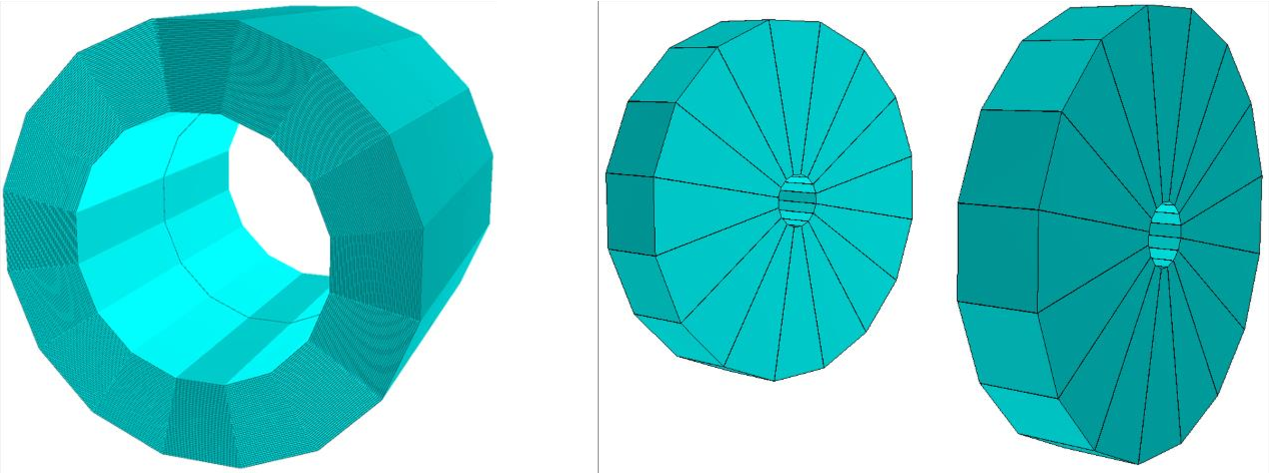
\includegraphics[width=0.9\textwidth]{Geometry.pdf}
\caption{Geometric configuration of the GS-HCAL system.
Left: barrel with 16~trapezoidal sectors forming a cylindrical structure
(inner diameter \SI{4280}{mm}, outer diameter \SI{6910}{mm}).
Right: endcap disks with matching sector segmentation.}
\label{fig:GS-geometry}
\end{figure}

%% ====================================================================
\section{Design requirements and baseline rationale}
\label{sec:rationale}
%% ====================================================================

The adoption of the GS-HCAL as the baseline HCAL of the CEPC
reference detector rests on the convergence of three independent lines
of argument: the physics requirements imposed by the CEPC programme
and the PFA paradigm; the technology requirements that any candidate
HCAL must simultaneously satisfy; and the specific combination of
measured and simulated properties that makes GS-HCAL the most mature
integrated technology satisfying all of them together.

%% --------------------------------------------------------------------
\subsection{Physics-driven requirements}
\label{subsec:physics-req}
%% --------------------------------------------------------------------

In the PFA paradigm the HCAL must independently measure neutral
hadrons---primarily neutrons and $K_{L}^{0}$ mesons---that leave no
tracks in the central tracker and carry approximately 10\% of the jet
energy.
These particles are the dominant source of resolution degradation in
PFA jet reconstruction, because their energy must be taken directly
from the calorimeter rather than from the tracker.
The CEPC target BMR of 3--4\% for $W/Z$/Higgs dijet final states
therefore translates into stringent HCAL requirements:
\begin{itemize}
\item Fine three-dimensional granularity is required to separate
  neutral-hadron clusters from nearby charged-particle energy deposits
  and to enable longitudinal shower analysis.
\item Sufficient depth, typically $\gtrsim6\,\lambdaI$ in the
  HCAL~itself, is required to contain hadronic showers and minimise
  longitudinal leakage.
\item The energy response must be close to linear and well-calibrated
  across the relevant range (${\sim}0.5$--\SI{60}{GeV}) so that PFA
  reconstruction of jet substructure remains robust.
\item Good single-hadron resolution also benefits searches for
  long-lived particles that may decay within the HCAL volume.
\end{itemize}

%% --------------------------------------------------------------------
\subsection{Technology-driven requirements}
\label{subsec:tech-req}
%% --------------------------------------------------------------------

Any HCAL technology candidate for the CEPC reference detector must
simultaneously satisfy the following integrated requirements:

\begin{itemize}
\item \textbf{Active-medium density:} higher density reduces the
  detector envelope for a fixed number of nuclear interaction lengths,
  which is critical in the limited radial budget of the reference
  detector.
\item \textbf{Cell granularity at the $40\times40$~mm$^{2}$ scale:}
  required for PFA shower separation; must be reproducibly
  manufacturable at that scale.
\item \textbf{SiPM-compatible light output:} the active medium must
  produce enough scintillation light that a compact SiPM readout can
  operate at a \SI{0.1}{MIP} threshold while suppressing dark-count
  noise.
\item \textbf{Scalability to approximately 5.22~million channels:} the
  production, assembly, and quality-control procedures must be
  compatible with the resulting system-level complexity.
\item \textbf{Radiation tolerance:} optical performance must be
  retained under the accumulated doses expected during Higgs and
  $Z$-pole operation.
\item \textbf{Thermal and electronics integration:} the front-end
  electronics, cooling, and mechanical support must be accommodated
  within the available layer thickness.
\item \textbf{Modular assembly feasibility:} the detector must be
  buildable, installable, and serviceable at realistic engineering
  tolerances.
\end{itemize}

These requirements must be satisfied \emph{together}---a technology
that excels in only a subset of them is not a viable baseline.

%% --------------------------------------------------------------------
\subsection{Why GS-HCAL is adopted as the baseline}
\label{subsec:why-baseline}
%% --------------------------------------------------------------------

The GS-HCAL is adopted as the baseline because the combined evidence
from materials R\&D, single-cell measurements, full-detector
digitisation simulation, and engineering analysis shows that it is the
most mature technology that satisfies the requirements of
Sections~\ref{subsec:physics-req} and~\ref{subsec:tech-req}
simultaneously.
The supporting evidence is of three distinct types, which are kept
separate throughout this paper:
(A)~experimentally measured properties of GFO cells and SiPM readout;
(B)~full-detector Geant4 digitisation simulation of the baseline
geometry; and (C)~analyses whose final closure depends on ongoing
prototype beam tests.

Specifically, the baseline choice is supported by the following five
points.

\begin{enumerate}
\item \textbf{Active-medium density (A).}
  GFO glass provides a density of \SI{6.0}{g/cm^{3}}, substantially
  higher than plastic scintillator (${\sim}\SI{1.03}{g/cm^{3}}$),
  while remaining manufacturable at the $40\times40\times10$~mm$^{3}$
  cell scale and delivering a measured intrinsic light yield
  $>\SI{1000}{\phMeV}$ (Sections~\ref{subsec:gfo}
  and~\ref{subsec:lightyield}).
\item \textbf{Cell geometry and PFA compatibility (A+B).}
  The \cellsize cell geometry, combined with \sipmsize SiPM readout,
  is compatible with highly granular PFA calorimetry; measured
  single-cell light outputs of 60--100~\peMIP
  (Section~\ref{subsec:cellmeas}) establish that practical SiPM
  operation is achievable at the required threshold.
\item \textbf{Radiation tolerance (A).}
  The GFO light yield retains more than 70\% of its initial value at
  \SI{100}{Gy} (Section~\ref{subsec:radiation}), which covers the
  accumulated dose expected over the CEPC operational scenarios.
\item \textbf{Projected detector performance (B).}
  Full digitisation-based Geant4 simulation of the baseline geometry
  predicts a single-hadron energy resolution of
  $\sigma_{E}/E = 29.8\%/\sqrt{E}\oplus6.5\%$ and an $H\to gg$ BMR of
  3.88\%, consistent with the CEPC target of 3--4\%
  (Sections~\ref{subsec:hadronres} and~\ref{subsec:physperf}).
\item \textbf{Detector-scale feasibility (A+B).}
  Finite-element analysis of the modular-box architecture demonstrates
  mechanical feasibility under the full load including the ECAL, and
  the water-cooling and calibration concepts are compatible with the
  channel count and dissipation
  (Sections~\ref{subsec:architecture}--\ref{subsec:channels}
  and~\ref{subsec:mechanics}).
\end{enumerate}

Categories~A and~B together establish the technical basis of the
baseline.
Final experimental closure, category~C, requires prototype beam tests
and is the subject of Section~\ref{subsec:prototype}.

%% --------------------------------------------------------------------
\subsection{Boundaries and remaining work}
\label{subsec:boundaries}
%% --------------------------------------------------------------------

The baseline rationale is transparent about what has \emph{not} yet
been experimentally closed.
Before proceeding to the detailed design and characterisation, the
principal boundaries of the current evidence are summarised here:

\begin{itemize}
\item Full prototype beam validation has not yet been performed; the
  8112-channel prototype is under construction
  (Section~\ref{subsec:prototype}).
\item The Geant4 optical model of GFO requires further tuning: the
  simulated single-cell light yield (${\sim}42$~\peMIP) is lower
  than the cosmic-ray measurement (${\sim}64$~\peMIP)
  (Section~\ref{subsec:optsim}).
\item The Birks constant used in the digitisation model is
  preliminary; a dedicated heavy-ion measurement is planned
  (Section~\ref{subsec:simsetup}).
\item The intrinsic $e/h$ compensation ratio has not yet been
  extracted from shower-component decomposition
  (Section~\ref{subsec:eresponse}).
\item The constant term (${\approx}5$--6\%) is currently dominated by
  longitudinal leakage in the $6\,\lambdaI$ design
  (Section~\ref{subsec:constterm}).
\item Tile production yield and light-yield uniformity still require
  optimisation: at present only about 60\% of produced tiles exceed
  the \SI{1000}{\phMeV} target (Section~\ref{subsec:qc}).
\end{itemize}

These items are discussed systematically in
Section~\ref{sec:discussion}.
They define the validation path of the baseline, but they do not
invalidate the baseline choice itself: a baseline identifies the most
mature and best-supported integrated technology direction, not a
concept whose every uncertainty is already experimentally closed.

%% ====================================================================
\section{Baseline detector concept and system design}
\label{sec:design}
%% ====================================================================

The baseline concept is realised at detector scale through a
barrel-plus-endcap architecture with 48~longitudinal layers of
\cellsize GFO cells.
Each design choice is driven by one or more of the requirements
established in Section~\ref{sec:rationale}, and the motivation is
given before the corresponding parameters.

%% --------------------------------------------------------------------
\subsection{Overall architecture}
\label{subsec:architecture}
%% --------------------------------------------------------------------

The overall architecture is driven by three requirements:
hermetic geometric coverage for PFA, sufficient depth for hadronic
containment, and a granularity compatible with shower separation in
the CEPC jet environment.
These requirements are met by a barrel with two endcaps, each
segmented into 16~trapezoidal sectors of 48~longitudinal layers and a
total depth of $6\,\lambdaI$ in steel and GS
(Figure~\ref{fig:GS-geometry}).
The barrel has inner and outer radii of \SI{2140}{mm} and
\SI{3455}{mm} and a length of \SI{6460}{mm} along the beam axis; the
endcaps match this segmentation with inner and outer radii of
\SI{450}{mm} and \SI{3455}{mm}.
The complete detector contains approximately 5.22~million identical
\cellsize GFO cells, each read out by a \sipmsize SiPM; the
corresponding sampling fraction is approximately 31\%.

%% --------------------------------------------------------------------
\subsection{Single-layer design as the fundamental baseline unit}
\label{subsec:onelayer}
%% --------------------------------------------------------------------

The single-layer design is the fundamental unit of the baseline
detector concept.
It is chosen so that the active GS layer, the SiPM plus PCB readout,
the ASIC cooling, and the steel absorber all fit within a compact
layer thickness while preserving the sampling fraction and mechanical
tolerances required by the PFA design.
Each layer has a total thickness of \SI{27.2}{mm}, corresponding to
approximately $0.125\,\lambdaI$, and contains from top to bottom:
a \SI{2}{mm} upper cover plate;
the \SI{10}{mm} GS active layer of $40\times40$~mm$^{2}$ cells;
a \SI{3.2}{mm} PCB layer carrying the front-end ASICs;
a \SI{2}{mm} bottom cover; and
a \SI{9.8}{mm} steel absorber in which cooling pipes of \SI{3}{mm}
outer radius are embedded.
One SiPM is positioned at the centre of each GS cell on a PCB shared
by multiple cells.
The nuclear-interaction-length contributions of the steel absorber,
the GS active layer, and the PCB are in the ratio $1:0.53:0.03$,
giving a sampling fraction of approximately 31\%.

\begin{figure}[htbp]
\centering
\begin{subfigure}{0.50\linewidth}
  \centering
  \includegraphics[width=\linewidth]{GS-HCAL-cell.pdf}
  \caption{}
  \label{fig:gshcal-cell-a}
\end{subfigure}%
\begin{subfigure}{0.35\linewidth}
  \centering
  \includegraphics[width=\linewidth]{GSHCALOneCell1.pdf}
  \caption{}
  \label{fig:gshcal-cell-b}
\end{subfigure}
\caption{(a)~Single-layer structure of the GS-HCAL\@.
(b)~One GS cell of \cellsize.}
\label{fig:gshcal-cell}
\end{figure}

%% --------------------------------------------------------------------
\subsection{Barrel implementation}
\label{subsec:barrel}
%% --------------------------------------------------------------------

The barrel is divided into 16~trapezoidal sectors
(Figure~\ref{fig:BarrelContourDimension}), each having a front width
of \SI{851}{mm}, a back width of \SI{1375}{mm}, and a radial thickness
of \SI{1315}{mm} ($6\,\lambdaI$).
The longitudinal segmentation into 48~layers follows the PFA
optimisation performed with the Plastic-Scintillator HCAL
prototype~\cite{CALICE:2010fpb}.
The total barrel weight is \SI{955}{t}
(Table~\ref{tab:BarrelWeight}).

Each layer consists of a continuous steel absorber plate over the full
barrel length, onto which modular detection boxes are mounted.
Each box contains a complete detection unit---GS cells, SiPMs, PCB,
ASICs, cables, and cover plates---with three standard box widths
(\SI{320}{mm}, \SI{280}{mm}, \SI{240}{mm}) combined to follow the
trapezoidal geometry while preserving the uniform \cellsize~cell
granularity (Figure~\ref{fig:BarrelModuleStructure}).
The 16~radial sector boundaries introduce projective cracks, but these
are effectively compensated by the upstream BGO ECAL
(${\approx}1.2\,\lambdaI$), which initiates most hadronic showers
before the HCAL and produces lateral spread bridging the sector
boundaries.

\begin{figure}[htbp]
\centering
\begin{subfigure}{0.42\linewidth}
  \centering
  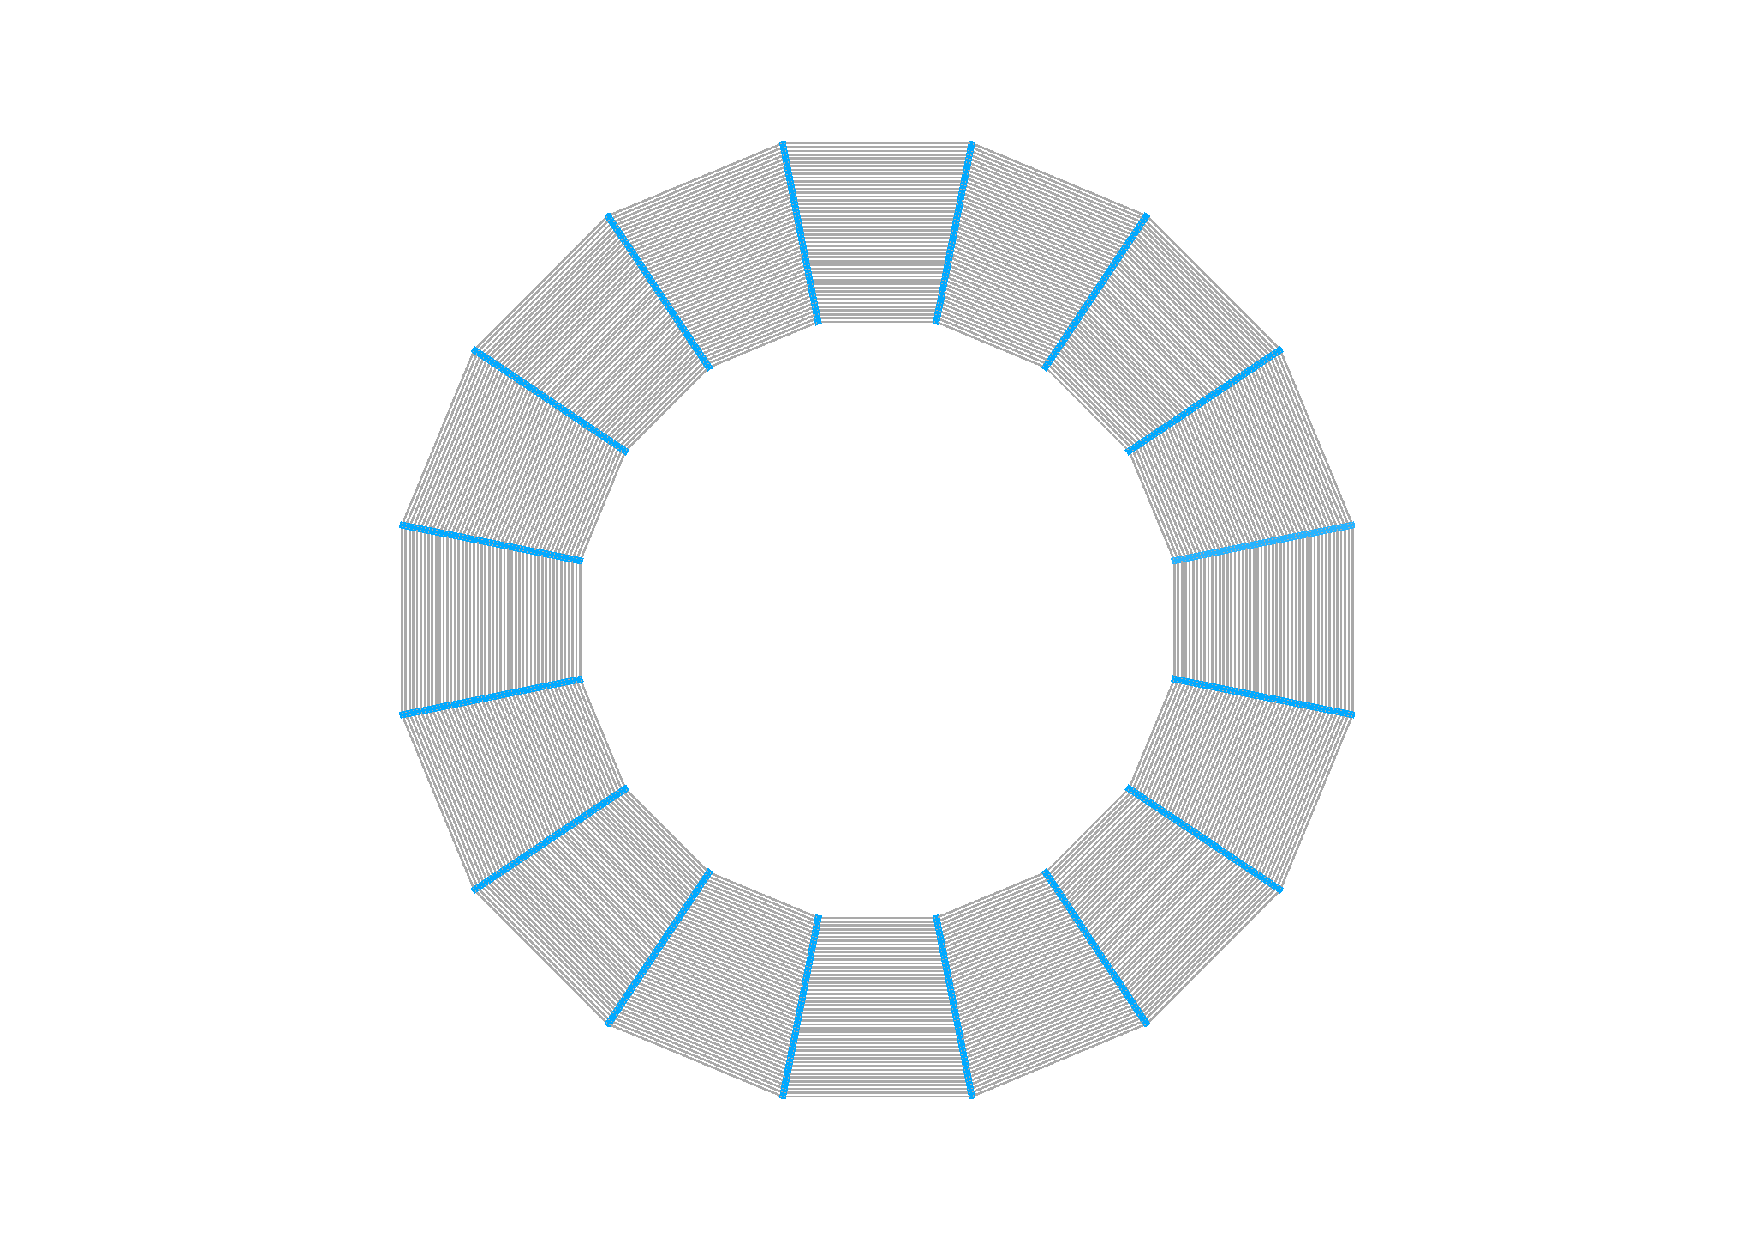
\includegraphics[width=\linewidth,trim=160pt 50pt 160pt 50pt,clip]{BarrelView1.pdf}
  \caption{}
\end{subfigure}\hfill
\begin{subfigure}{0.45\linewidth}
  \centering
  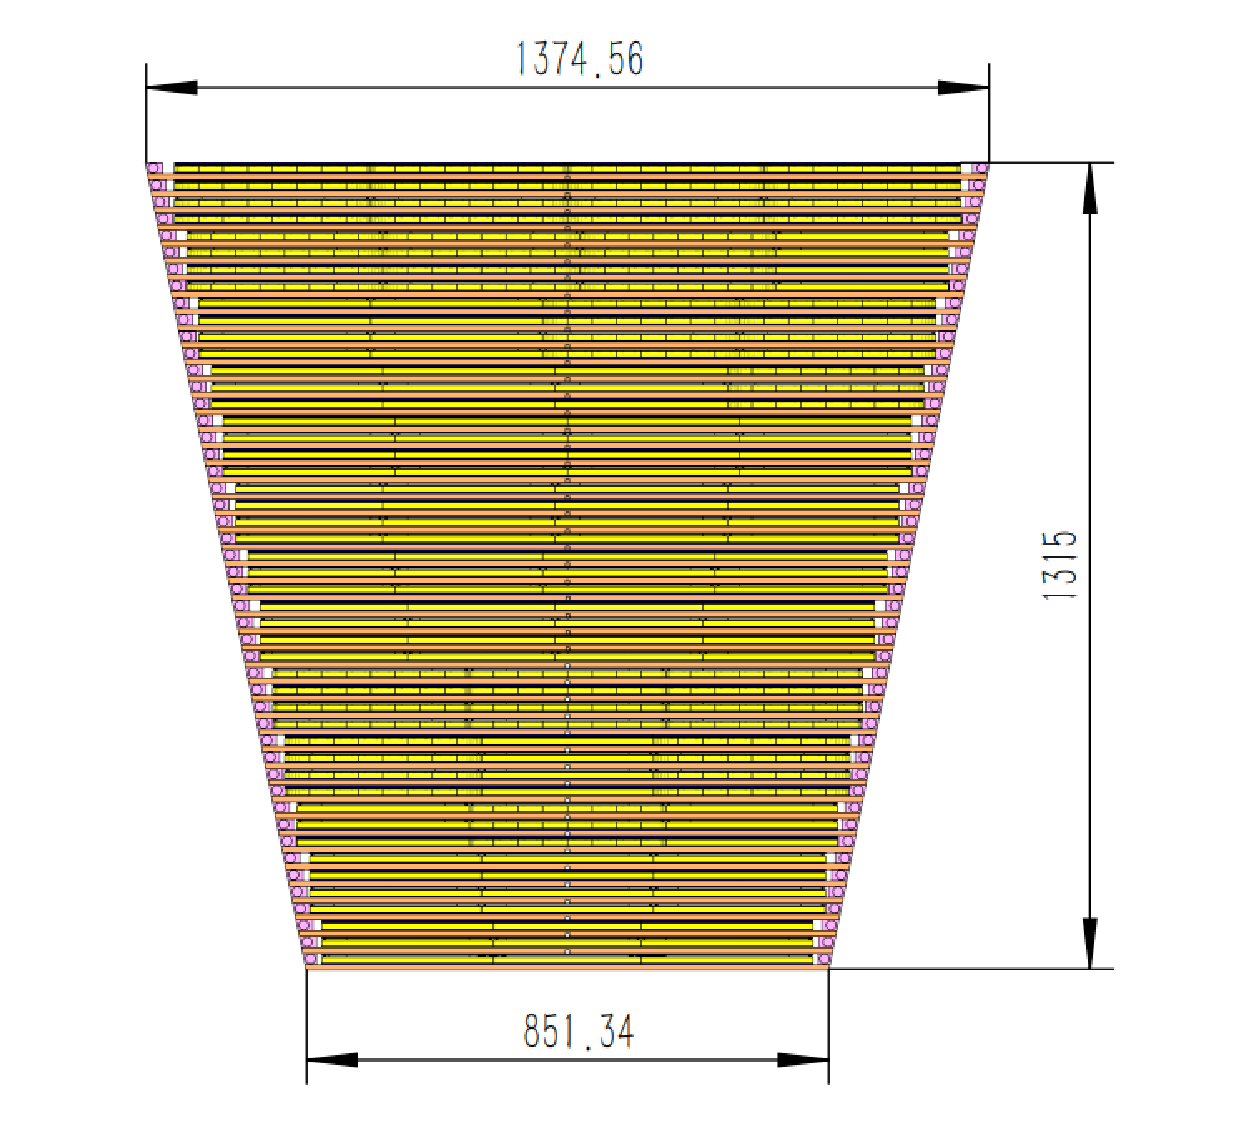
\includegraphics[width=\linewidth]{HCALBarrelOneSector.pdf}
  \caption{}
\end{subfigure}
\caption{Dimensions of the GS-HCAL barrel.
(a)~Cross-sectional view showing 16~trapezoidal sectors
(inner diameter \SI{4280}{mm}, outer diameter \SI{6910}{mm}).
(b)~Side view of a single trapezoidal sector.}
\label{fig:BarrelContourDimension}
\end{figure}

\begin{figure}[htbp]
\centering
\includegraphics[width=0.9\linewidth]{Fig.1.81-Boxes_dimension-and_more-structure_details.pdf}
\caption{GS-HCAL barrel sector structure.
(a)~Full sector composed of 48~layers.
(b)~Dimensions of an individual box.
(c)~Internal structure of a box with cover plates, GS cells, PCB
with ASICs, cables, and cooling-water pipes.}
\label{fig:BarrelModuleStructure}
\end{figure}

\begin{table}[htbp]
\centering
\caption{Weight breakdown of the barrel GS-HCAL\@.}
\label{tab:BarrelWeight}
\begin{tabular}{l S[table-format=5.0] S[table-format=3.1]}
\toprule
\textbf{Component} & {\textbf{Weight/sector (kg)}} & {\textbf{Weight/barrel (t)}} \\
\midrule
Cover plate        & 10287 & 164.6 \\
PCB plate          &   390 &   6.2 \\
Glass scintillator & 19277 & 308.4 \\
Absorber layer     & 27515 & 440.2 \\
Support structure  &  1883 &  30.1 \\
Auxiliaries        &   350 &   5.6 \\
\midrule
Total              & 59702 & 955.2 \\
\bottomrule
\end{tabular}
\end{table}

%% --------------------------------------------------------------------
\subsection{Endcap implementation}
\label{subsec:endcap}
%% --------------------------------------------------------------------

The two endcaps complete the geometric coverage along the beam
direction (Figure~\ref{fig:EndcapsOverall}).
Each endcap mirrors the barrel segmentation with 16~disk-shaped
sectors, inner and outer radii of \SI{450}{mm} and \SI{3455}{mm}, and a
total thickness of \SI{1315}{mm} in 48~layers.
A single sector has a top width of \SI{1307}{mm} and a radial height of
\SI{2862}{mm}, and is divided radially into six boxes.
Each endcap weighs \SI{362}{t}.

\begin{figure}[htbp]
\centering
\begin{subfigure}{0.58\linewidth}
  \centering
  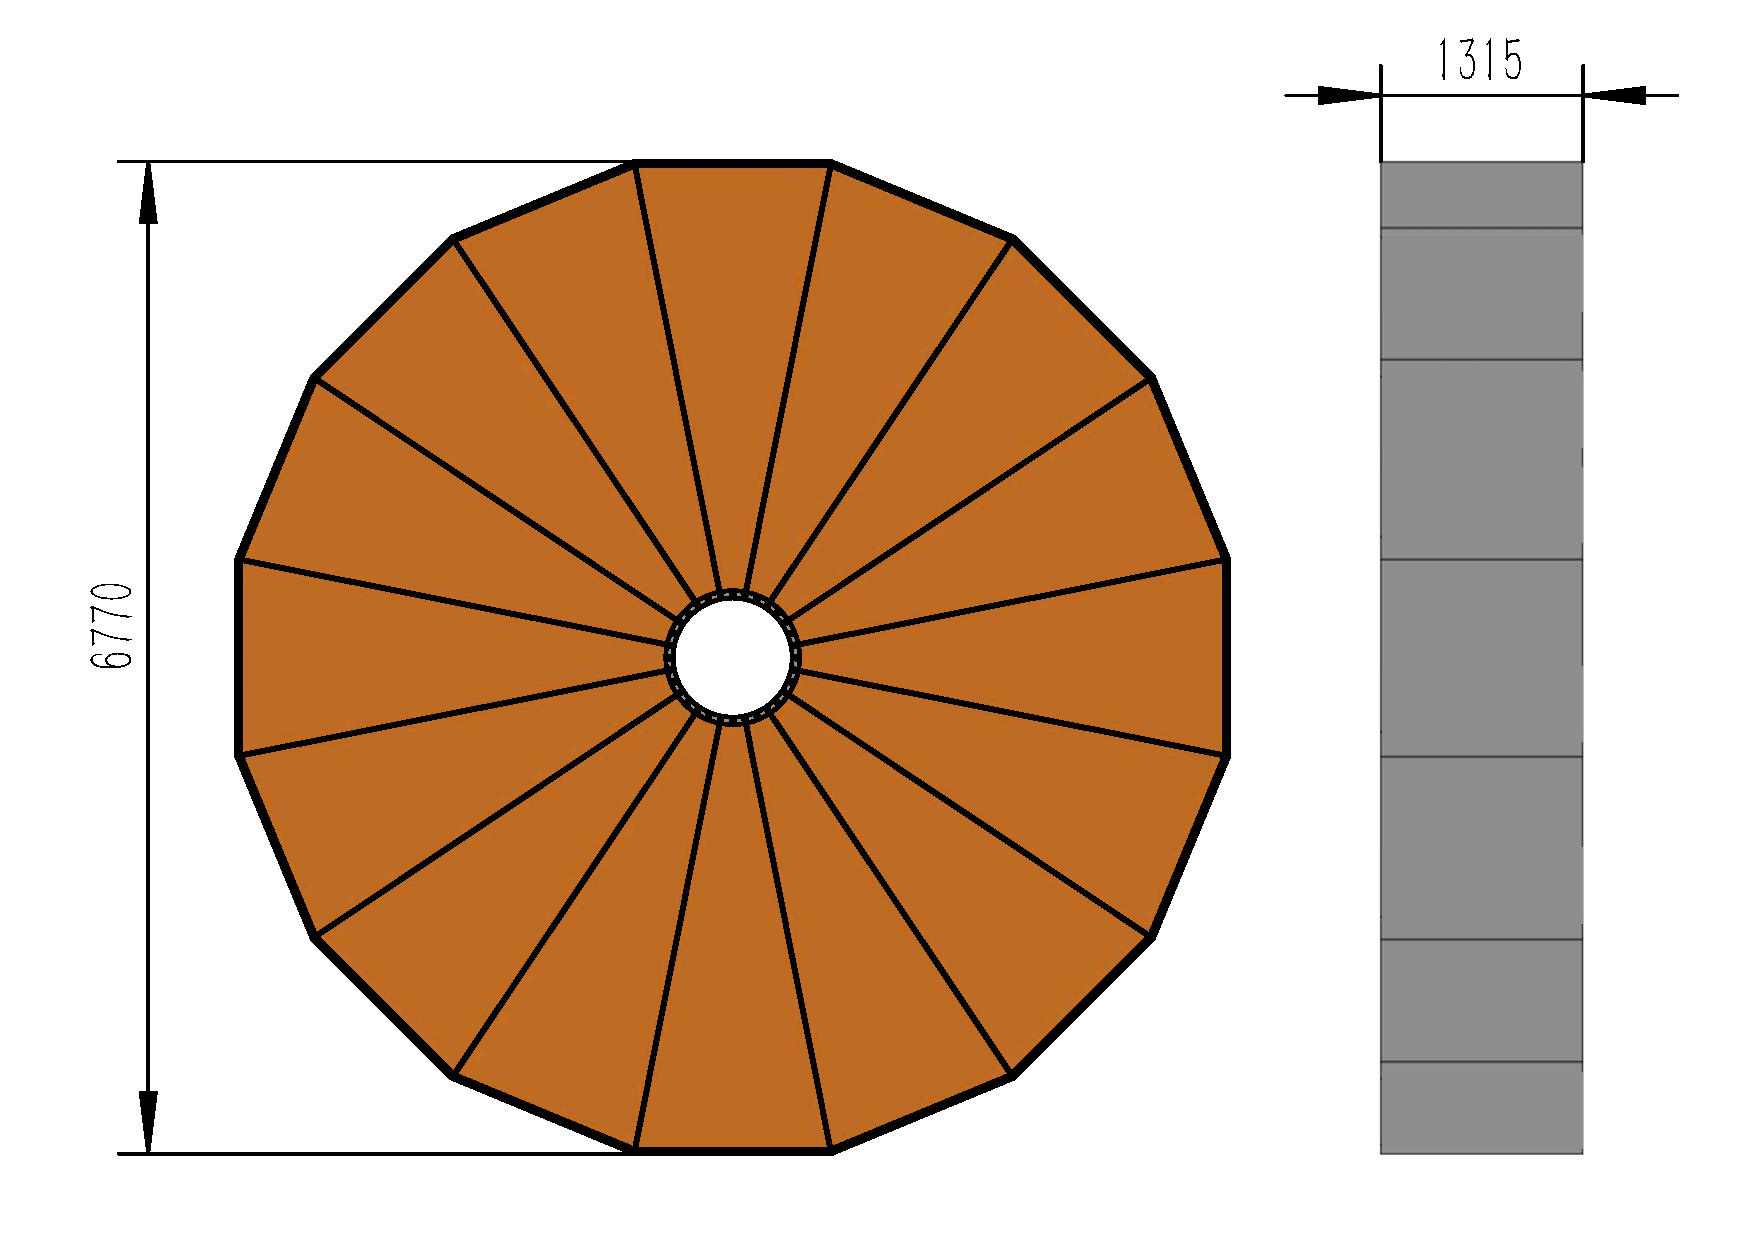
\includegraphics[width=\linewidth]{HCALEndcapOverall.pdf}
  \caption{}
\end{subfigure}\hfill
\begin{subfigure}{0.20\linewidth}
  \centering
  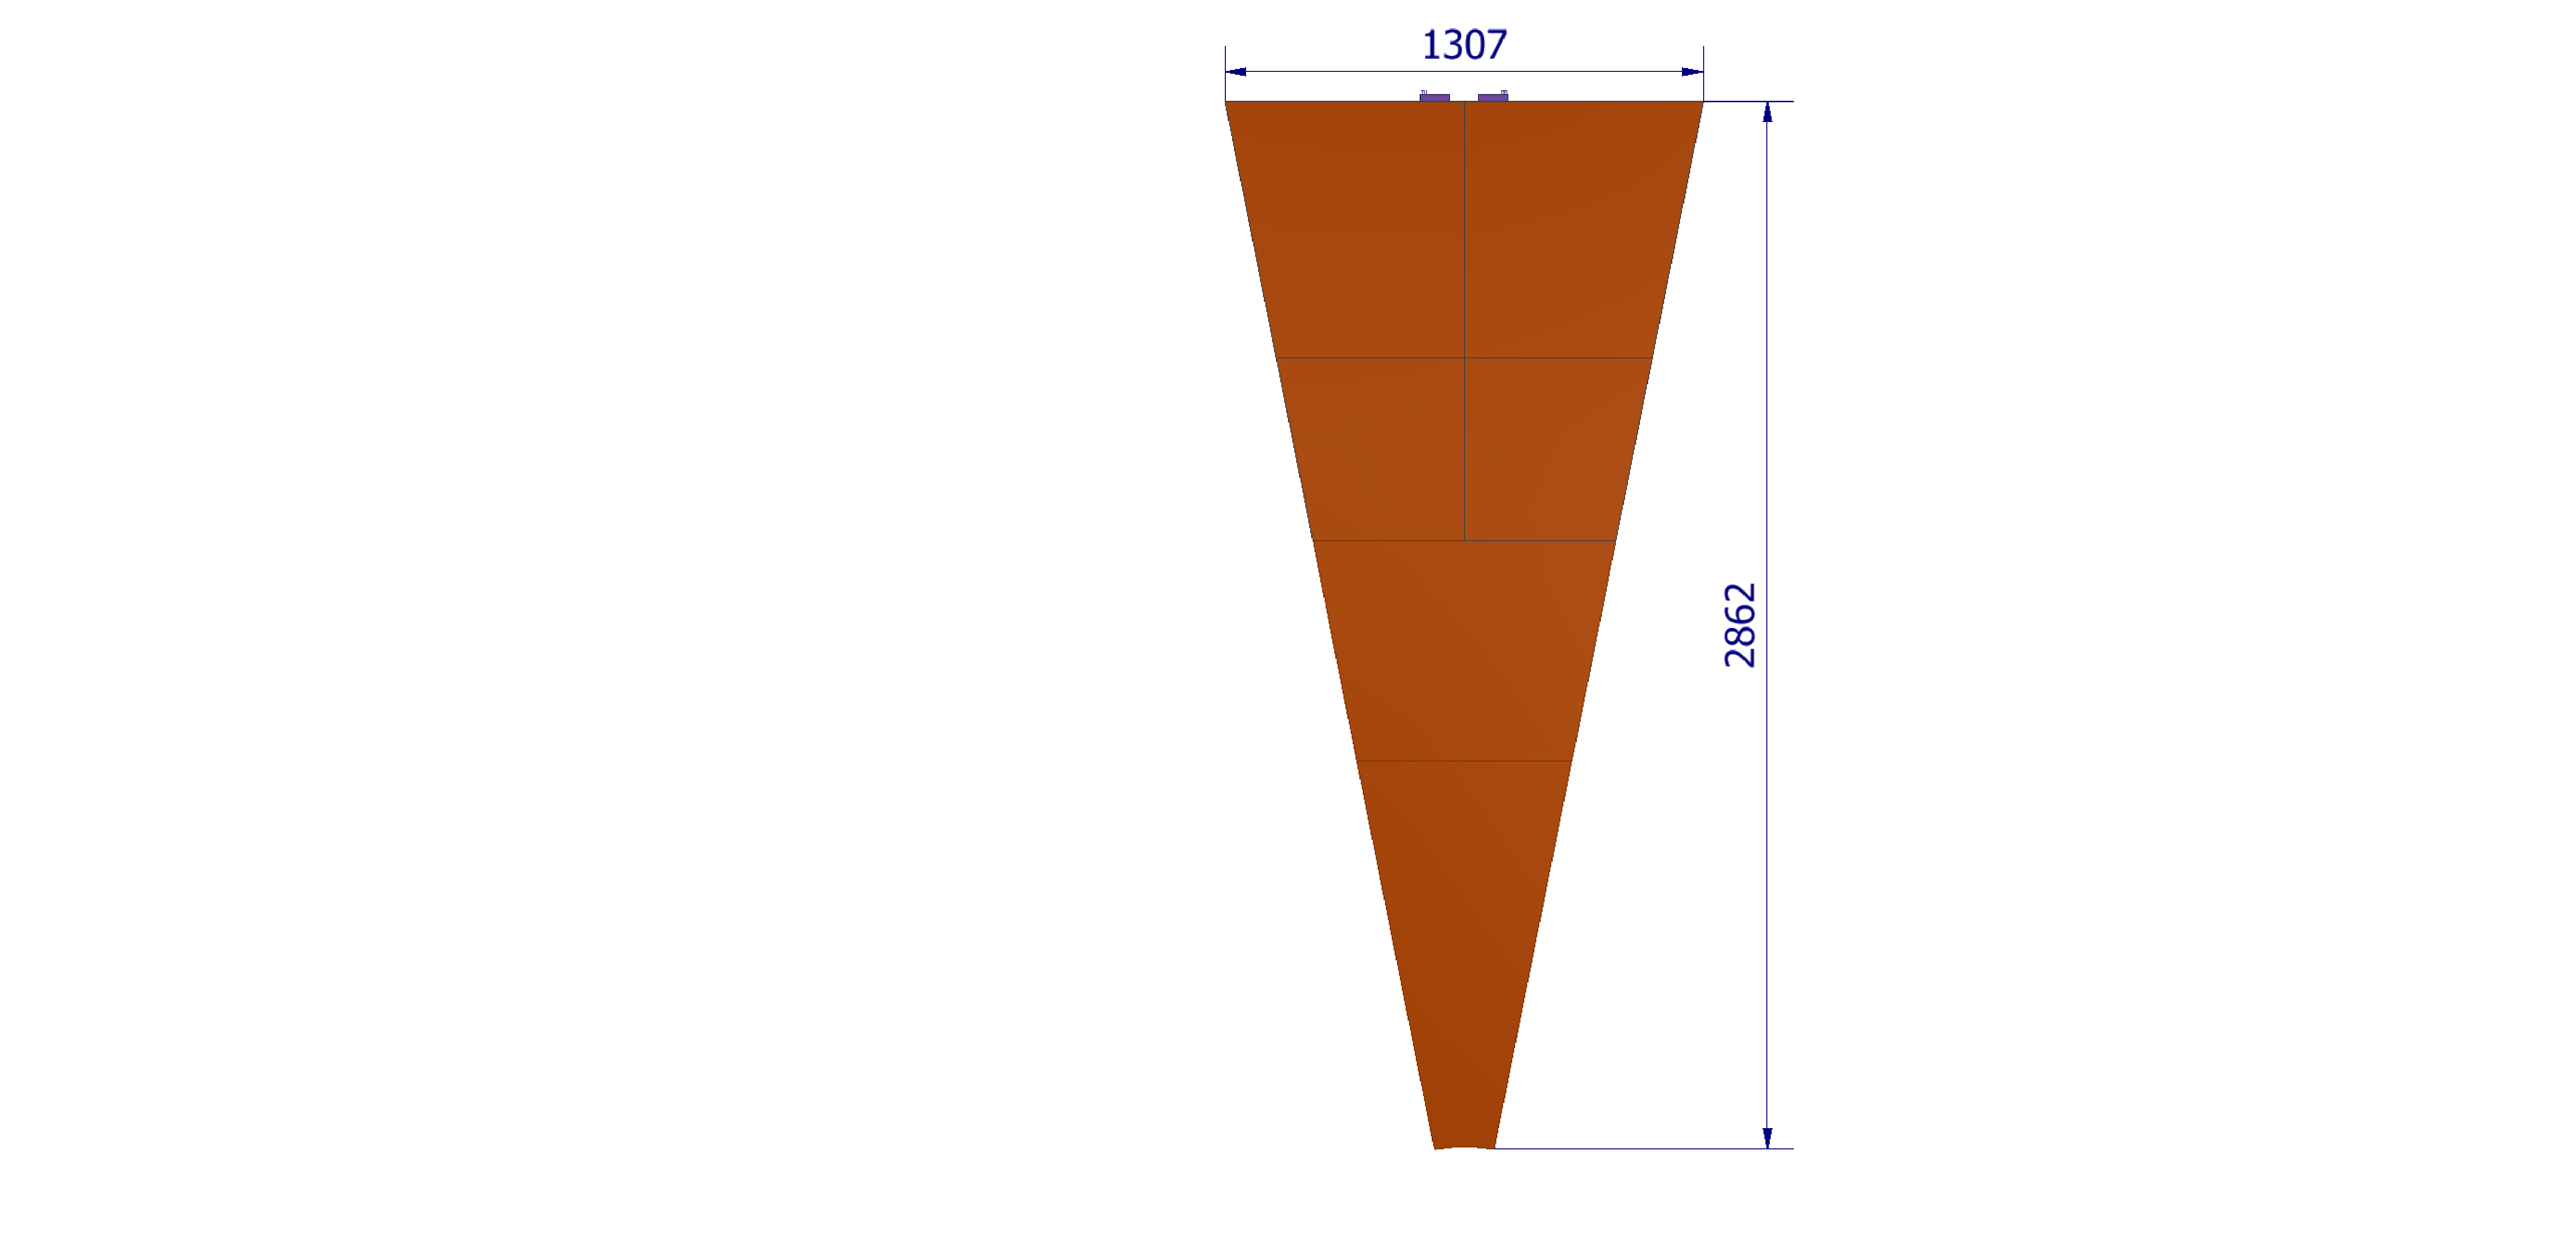
\includegraphics[width=\linewidth]{HCALEndcapOneSector.pdf}
  \caption{}
\end{subfigure}
\caption{Dimensions of the GS-HCAL endcaps.
(a)~Front and side views.
(b)~A single endcap sector.}
\label{fig:EndcapsOverall}
\end{figure}

%% --------------------------------------------------------------------
\subsection{Services: cooling, routing, and modular assembly}
\label{subsec:cooling}
%% --------------------------------------------------------------------

Service integration is an integral part of the baseline concept
because the 5.22~million channels and \SI{15}{mW/channel} ASIC power
impose non-trivial thermal and routing constraints on any practical
realisation.
A water-cooling system manages the front-end thermal load.
In the barrel, four cooling pipes are embedded in the steel absorber
of each layer, and every eight consecutive layers share common
manifolds to form six independent cooling loops per sector
(Figure~\ref{fig:BarrelCooling}).
In the endcap, 16~cooling regions per layer connect vertically across
all 48~layers to form 48~parallel circuits
(Figure~\ref{fig:M-14}).
The modular box architecture, combined with the eight-in-one cooling
topology, also provides clear routing paths for cables and gas, and
supports in-layer access during assembly and maintenance.

\begin{figure}[htbp]
\centering
\begin{subfigure}{0.55\linewidth}
  \centering
  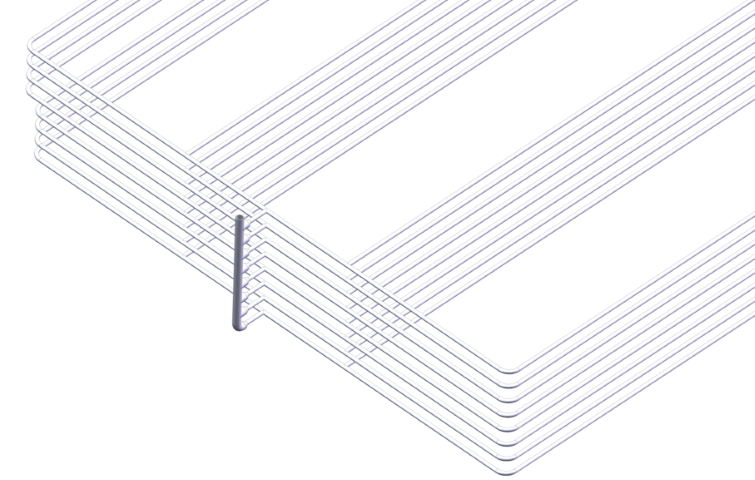
\includegraphics[width=\linewidth]{CoolingBarrelLeft.png}
  \caption{}
\end{subfigure}\hfill
\begin{subfigure}{0.35\linewidth}
  \centering
  \includegraphics[width=\linewidth]{CoolingBarrelv2.jpg}
  \caption{}
\end{subfigure}
\caption{Cooling-pipe routing for a barrel sector.
(a)~Schematic of the eight-in-one pipeline design.
(b)~Simulated coolant flow-velocity distribution.}
\label{fig:BarrelCooling}
\end{figure}

\begin{figure}[htbp]
\centering
\begin{subfigure}{0.50\linewidth}
  \centering
  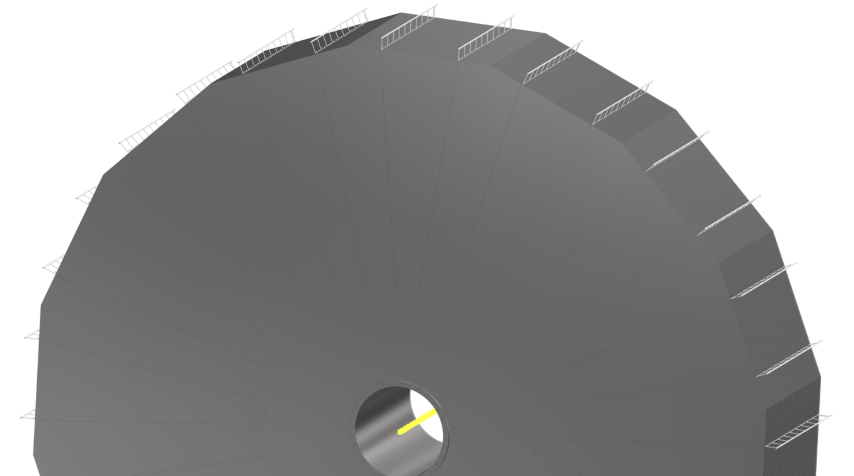
\includegraphics[width=\linewidth]{CoolingEndcapHalf.png}
  \caption{}
\end{subfigure}\hfill
\begin{subfigure}{0.42\linewidth}
  \centering
  \raisebox{0.1cm}{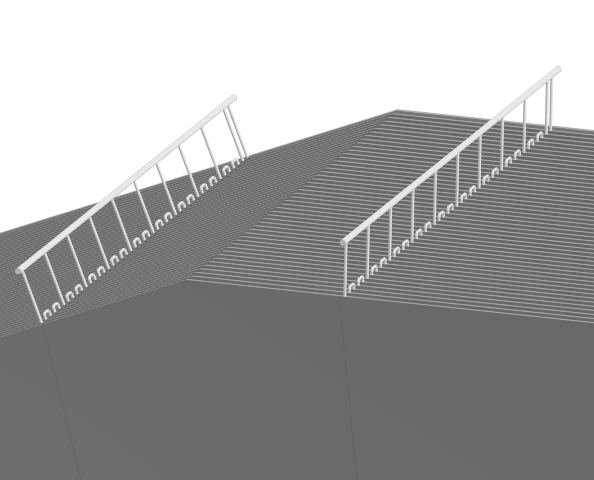
\includegraphics[width=\linewidth]{CoolingEndcapPart.png}}
  \caption{}
\end{subfigure}
\caption{Endcap cooling-pipe structure: (a)~half of the endcap;
(b)~zoomed corner view.}
\label{fig:M-14}
\end{figure}

%% --------------------------------------------------------------------
\subsection{Channel count and detector-scale implications}
\label{subsec:channels}
%% --------------------------------------------------------------------

Table~\ref{tab:GSHCALQuantities} summarises the cell, box, layer, and
sector counts.
The complete detector contains approximately 5.22~million readout
channels.
This number is itself a baseline-level design constraint:
it fixes the scale of ASIC production, calibration infrastructure
(Section~\ref{subsec:calibration}), and modular assembly
(Section~\ref{subsec:prototype}), and it is the principal driver of the
low-power per-channel requirement.
The baseline numbers are therefore chosen so that each of these
detector-scale dependencies is simultaneously feasible rather than
optimised independently.

\begin{table}[htbp]
\centering
\caption{Numbers of cells, boxes, layers, and sectors for the barrel
and the two endcaps.}
\label{tab:GSHCALQuantities}
\begin{tabular}{lcccc}
\toprule
\textbf{Part} & \textbf{Cells} & \textbf{Boxes} & \textbf{Layers} &
\textbf{Sectors} \\
\midrule
Barrel             & 3\,212\,800          & 27\,840        & $48\times16$
& 16 \\
Endcap ($\times2$) & $1\,006\,080\times2$ & $3072\times2$  &
$48\times16\times2$ & $16\times2$ \\
\bottomrule
\end{tabular}
\end{table}

%% ====================================================================
\section{Glass scintillator, photosensor, and front-end implementation}
\label{sec:activeunit}
%% ====================================================================

The baseline active unit---the GFO cell, the SiPM, the front-end
electronics, and the supporting optical simulation---constitutes the
primary technology chain of the GS-HCAL.
Each component is characterised as part of this integrated chain,
because the performance of any element is meaningful only in the
context of the others.

%% --------------------------------------------------------------------
\subsection{Choice of GFO glass as the baseline active medium}
\label{subsec:gfo}
%% --------------------------------------------------------------------

High-$Z$ glass scintillators have been investigated for calorimetry
since the 1980s~\cite{Buchner:1988fu}, but early attempts were limited
by short radiation length, low light yield, and strong self-absorption
in long-bar geometries.
The maturation of SiPM technology and PFA-oriented highly granular
calorimetry changed this picture: compact optically isolated cells of
${\sim}\SI{1}{cm}$-scale thickness eliminate the long-path
self-absorption problem, so that a moderate light yield of
${\sim}\SI{1000}{\phMeV}$ combined with a modern SiPM becomes
sufficient for practical readout~\cite{Tang:2022yrb,Hu:2023dbm,
Hu:2024nvo}.

Building on this opportunity, the Glass-Scintillator Collaboration has
systematically developed high-$Z$ glass
compositions~\cite{LAN2022113000,YU2023113846,ZHU2024} targeting the
density--light-yield trade-off with manufacturability at the
\cellsize cell scale (Figure~\ref{fig:GSGroup}).
Gadolinium fluoro-oxide (GFO) glass is adopted as the baseline active
medium because it combines high density, manufacturable tile geometry,
and adequate optical properties in a single
material~\cite{HUA202523367,Hua:2023myf,Hua:2024djh}.
Its key parameters are listed in Table~\ref{tab:GS1} alongside BGO
crystal~\cite{BGO} and DSB glass~\cite{Dormenev:2021vtn} for
reference.
GFO achieves a density of \SI{6.0}{g/cm^{3}} with a radiation length of
\SI{1.59}{cm} and a nuclear interaction length of \SI{24.2}{cm}.
The Ce$^{3+}$ luminescent centre provides strong emission near
\SI{400}{nm} with efficient energy transfer from Gd$^{3+}$
modifiers~\cite{GS-1}; the borosilicate matrix provides thermal and
optical stability; and the use of gadolinium, rather than lanthanum or
lutetium, provides a favourable combination of density, intrinsic
radioactivity, and cost.
These properties are directly matched to the \cellsize cell
requirement.

\begin{figure}[htbp]
\centering
\includegraphics[width=0.7\textwidth]{GSGroup.pdf}
\caption{Light yield versus density for GS samples developed by the
Glass-Scintillator Collaboration and by other groups.}
\label{fig:GSGroup}
\end{figure}

\begin{table}[htbp]
\centering
\caption{Key parameters of GFO glass ($5\times5\times5$~mm$^{3}$
sample) compared with BGO crystal~\cite{BGO} and DSB
glass~\cite{Dormenev:2021vtn}.}
\label{tab:GS1}
\begin{tabular}{lccc}
\toprule
\textbf{Parameter} & \textbf{GFO} & \textbf{BGO} & \textbf{DSB} \\
\midrule
Density (g/cm$^{3}$)                       & 6.0      & 7.13  & 4.2   \\
Melting point ($^{\circ}$C)                 & 1250     & 1050  & 1550  \\
Radiation length (cm)                       & 1.59     & 1.12  & 2.62  \\
Moli\`{e}re radius (cm)                    & 2.49     & 2.23  & 3.33  \\
Nuclear interaction length (cm)             & 24.2     & 22.7  & 31.8  \\
$Z_{\mathrm{eff}}$                          & 56.6     & 71.5  & 49.7  \\
$dE/dx$ (MeV/cm)                            & 8.0      & 8.99  & 5.9   \\
Emission peak (nm)                          & 400      & 480   & 430   \\
Refractive index                            & 1.74     & 2.15  & ---   \\
Light yield (ph/MeV)                        & ${\sim}1500$ & 7500  & 2500  \\
Energy resolution (\% at \SI{662}{keV})     & ${\sim}23$   & 9.5   & ---   \\
Scintillation decay time (ns)               & ${\sim}60$, 500 & 60, 300 & 90, 400 \\
\bottomrule
\end{tabular}
\end{table}

%% --------------------------------------------------------------------
\subsection{Optical constraints and attenuation length}
\label{subsec:attenuation}
%% --------------------------------------------------------------------

The light attenuation length (LAL, $L_{0}$) is the key optical
parameter that determines whether a given cell geometry is viable for
SiPM readout at the centre of the cell.
The LAL is measured by thickness-dependent transmittance using
\begin{equation}
\label{eq:LAL}
L_{0} = \frac{L_{2}-L_{1}}{\ln(T_{L_{1}}/T_{L_{2}})},
\end{equation}
with two sample thicknesses $L_{1}<L_{2}$ and transmittances
$T_{L_{i}}$~\cite{Zhu:1996tt}.
The best-performing GFO sample yields
$L_{0}\approx\SI{6}{cm}$ at \SI{400}{nm}, the GS emission peak, and
remains between \SI{6}{cm} and \SI{6.8}{cm} across the visible
spectrum (Figure~\ref{fig:newLAL1}).

This value is compatible with the \cellsize baseline cell geometry.
The SiPM is mounted at the centre of the cell top surface, and the
longest straight optical path from a scintillation point to the sensor
is bounded by the cell diagonal,
$\sqrt{20^{2}+20^{2}+10^{2}}\approx\SI{30}{mm}$.
This is a factor of two smaller than the measured LAL, so first-pass
photon transport is dominated by geometric acceptance and Teflon
reflection rather than by bulk absorption.
The baseline attenuation length is therefore adequate for the cell
geometry; it does not require the centimetre-scale improvements that
would be mandatory in a long-bar readout.

\begin{figure}[htbp]
\centering
\includegraphics[width=0.60\textwidth]{NewLAL1.pdf}
\caption{Attenuation length of GFO glass versus wavelength, measured
using the transmittance method.}
\label{fig:newLAL1}
\end{figure}

%% --------------------------------------------------------------------
\subsection{SiPM selection and compatibility with the baseline cell}
\label{subsec:sipm}
%% --------------------------------------------------------------------

Silicon photomultipliers (SiPMs) are selected for the GS-HCAL readout
because of their compact form factor, high gain at low operating
voltage, radiation hardness, and insensitivity to magnetic fields.
They are already deployed in the CMS High-Granularity
Calorimeter~\cite{CMS:2017jpq} and CALICE highly granular
prototypes~\cite{calice}.
Four representative commercial devices from HPK, NDL, and JBT are
compared in Table~\ref{tab:SiPM-tab1}.

\begin{table}[htbp]
\centering
\caption{Parameters of commercial SiPMs evaluated for the GS-HCAL\@.}
\label{tab:SiPM-tab1}
\resizebox{\textwidth}{!}{%
\begin{tabular}{lcccc}
\toprule
\textbf{Supplier} & \multicolumn{2}{c}{\textbf{HPK}} &
\textbf{NDL} & \textbf{JBT} \\
\midrule
Type  & S14160-3015PS & S14160-3050HS & EQR20-11-3030-S & JSP-TP3050-SMT \\
Pixel pitch ($\upmu$m) & 15 & 50 & 20 & 50 \\
Number of pixels & 39\,984 & 3531 & 22\,500 & 3364 \\
Terminal capacitance (pF) & 530 & 500 & 157.5 & 0.170 \\
Breakdown voltage (V)
  & $38\pm3$ & $38\pm3$ & $27.2\pm1$ & $24.6\pm0.2$ \\
Recommended $V_{\mathrm{op}}$ (V)
  & $V_{\mathrm{BD}}+3$ & $V_{\mathrm{BD}}+2.7$
  & $V_{\mathrm{BD}}+5$ & $V_{\mathrm{BD}}+2$ \\
Peak-sensitivity wavelength (nm) & 450 & 450 & 420 & 420 \\
Peak PDE (\%) & 32 & 50 & 47.8 & 35 \\
PDE at \SI{400}{nm} (\%) & 27 & 47 & 45 & 33 \\
Gain & $3.6\times10^{5}$ & $2.5\times10^{6}$
     & $8.0\times10^{5}$ & $2.1\times10^{6}$ \\
DCR (kHz/mm$^{2}$) & 700--2100 & 10--100 & 150--450 & 120--270 \\
\bottomrule
\end{tabular}}
\end{table}

The selection is driven by four properties matched to the baseline
cell: high PDE at \SI{400}{nm} (matching the GFO emission peak);
sufficient gain for resolved photon counting; low dark count rate
(DCR); and cost compatible with millions of channels.

The central question for SiPM compatibility with the baseline cell is
whether the measured cell light output is large enough that a
threshold sufficient to suppress DCR can still be set well below one
MIP.
Figure~\ref{fig:ch08_SiPM_DCR} shows the DCR as a function of
photoelectron threshold for the candidate SiPMs.
With a measured cell output of ${\sim}60$~\peMIP, a \SI{0.1}{MIP}
threshold corresponds to approximately six photoelectrons.
At this threshold the DCR drops to approximately \SI{28}{Hz/mm^{2}}
(NDL~EQR20) and \SI{12}{Hz/mm^{2}} (HPK~S14160-3050)---well below the
expected hadronic event rate---demonstrating that the baseline cell
and commercial SiPMs together provide a practical
signal-to-noise margin.
The HPK~S14160-3050 and NDL~EQR20-11-3030 are therefore identified as
the most promising devices for the prototype phase.

\begin{figure}[htbp]
\centering
\includegraphics[width=0.60\textwidth]{SiPM_DCR_HCAL.pdf}
\caption{Dark count rate versus threshold level for several SiPM
models.}
\label{fig:ch08_SiPM_DCR}
\end{figure}

%% --------------------------------------------------------------------
\subsection{Front-end readout concept}
\label{subsec:fee}
%% --------------------------------------------------------------------

The baseline readout must eventually handle more than five million
SiPM channels with a dynamic range of 0.1--100~MIP, a charge
resolution of 10\% of 1~MIP, and an average event rate of
\SI{2}{kHz/channel}.
The resulting system-level requirements are summarised in
Table~\ref{tab:SiPM-tab3}.
A dedicated low-power ASIC meeting these specifications is under
development; it is one of the items that are expected to close with
the prototype.

\begin{table}[htbp]
\centering
\caption{SiPM-driven requirements for the readout electronics.}
\label{tab:SiPM-tab3}
\begin{tabular}{ll}
\toprule
\textbf{Parameter} & \textbf{Requirement} \\
\midrule
Charge dynamic range       & \SI{0.8}{pC}--\SI{800}{pC} (0.1--100~MIP) \\
Charge resolution          & 10\% of 1.0~MIP \\
SiPM capacitance           & $\leq\SI{100}{pF}$ \\
SiPM gain                  & $\geq5\times10^{5}$ \\
Average event rate/channel & \SI{2}{kHz} \\
Maximum event rate/channel & \SI{50}{kHz} \\
Typical signal amplitude   & 2--3~mV/p.e. \\
\bottomrule
\end{tabular}
\end{table}

For single-cell characterisation and prototype testing an interim
front-end solution was developed, because no commercial option
simultaneously met the baseline requirements~\cite{Wang:2023ffl}.
The interim pre-amplifier achieves a gain of $\pm\SI{20}{V/V}$, a
bandwidth of \SI{400}{MHz}, and a baseline noise of
$300\,\mu\mathrm{V}_\mathrm{RMS}$ at \SI{50}{\ohm} input impedance
(Figure~\ref{fig:SiPM_FEE}); this is sufficient to resolve
single-photoelectron peaks and to support all the single-cell
measurements of Section~\ref{sec:expchar}.

\begin{figure}[htbp]
\centering
\includegraphics[width=0.95\textwidth]{SiPM_FEE.pdf}
\caption{Pre-amplifier for the GS-HCAL SiPM readout.
(a)~Single-channel PCB coupled to a GS cell.
(b)~Schematic diagram.
(c,\,d)~Performance characteristics.
(e)~Waveform of a \sipmsize NDL SiPM (EQR20-11-3030D-S).
(f)~ADC spectrum of SiPM dark noise with well-separated
photoelectron peaks.}
\label{fig:SiPM_FEE}
\end{figure}

%% --------------------------------------------------------------------
\subsection{Optical simulation as design support}
\label{subsec:optsim}
%% --------------------------------------------------------------------

Geant4-based optical simulation~\cite{Tang:2022yrb} of a single
GS~cell coupled to a SiPM is used to support the design choices.
The simulation implements the baseline \cellsize cell with a single
\sipmsize SiPM at its centre, with the cell periphery wrapped in
Teflon reflective film; the physics list \texttt{QGSP\_BERT} is
combined with a full set of optical processes including scintillation,
Cherenkov radiation, Rayleigh scattering, bulk absorption, and
boundary effects.
Figure~\ref{fig:SiPM_MIPmap}(a) shows the simulated light-output
distribution for a cell with \SI{60}{mm} attenuation length, yielding
$42.05\pm0.01$~\peMIP; Figure~\ref{fig:SiPM_MIPmap}(b) shows the
expected dependence of the light output on the attenuation length
across 40, 60, and \SI{80}{mm}.

\begin{figure}[htbp]
\centering
\begin{subfigure}{0.43\textwidth}
  \centering
  \includegraphics[width=\linewidth]{Muon_GS_map_PDE60_3time3_AT6cmPE.pdf}
  \caption{}
\end{subfigure}\hfill
\begin{subfigure}{0.39\textwidth}
  \centering
  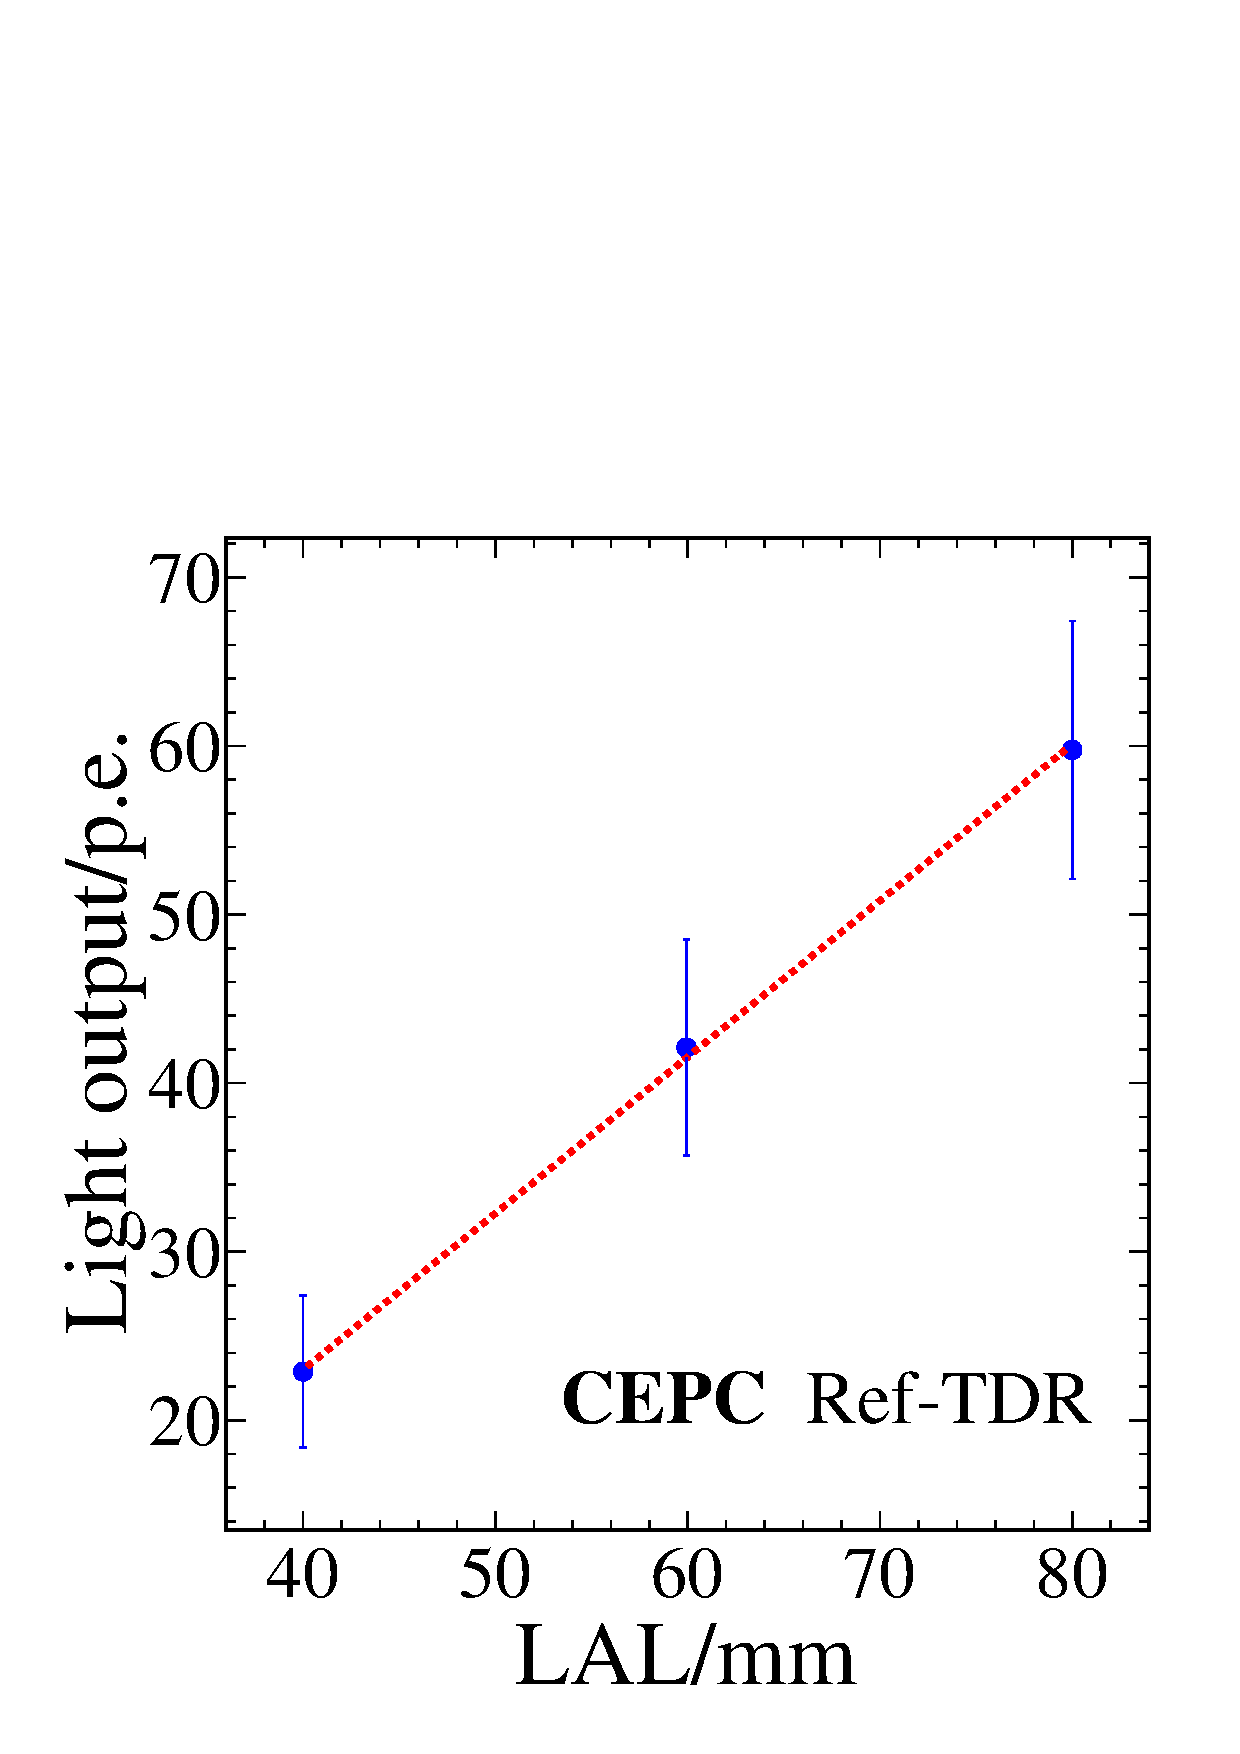
\includegraphics[width=\linewidth]{attenuation_fit.pdf}
  \caption{}
\end{subfigure}
\caption{(a)~Simulated light-output distribution of a GS cell with
\SI{60}{mm} attenuation length ($42.05\pm0.01$~\peMIP).
(b)~Fitted light-output MPV versus attenuation length.}
\label{fig:SiPM_MIPmap}
\end{figure}

Validation studies (Figure~\ref{fig:SiPM_SimValid}) show simulated
fast and slow scintillation components of \SI{96}{ns} and
\SI{1445}{ns}, somewhat longer than the measured reference values
of \SI{60}{ns} and \SI{500}{ns} (Table~\ref{tab:GS1}), and the
simulated single-muon light yield
(${\sim}\SI{42}{\peMIP}$) is lower than the measured cosmic-ray result
of ${\sim}\SI{64}{\peMIP}$ (Section~\ref{subsec:cellmeas}).
The optical simulation therefore plays a supporting role in the
baseline rationale rather than providing final experimental closure:
the current Geant4 optical model requires tuning against measured GFO
data, and this tuning is one of the immediate priorities of the
validation programme (Section~\ref{sec:discussion}).

\begin{figure}[htbp]
\centering
\begin{subfigure}{0.43\textwidth}
  \centering
  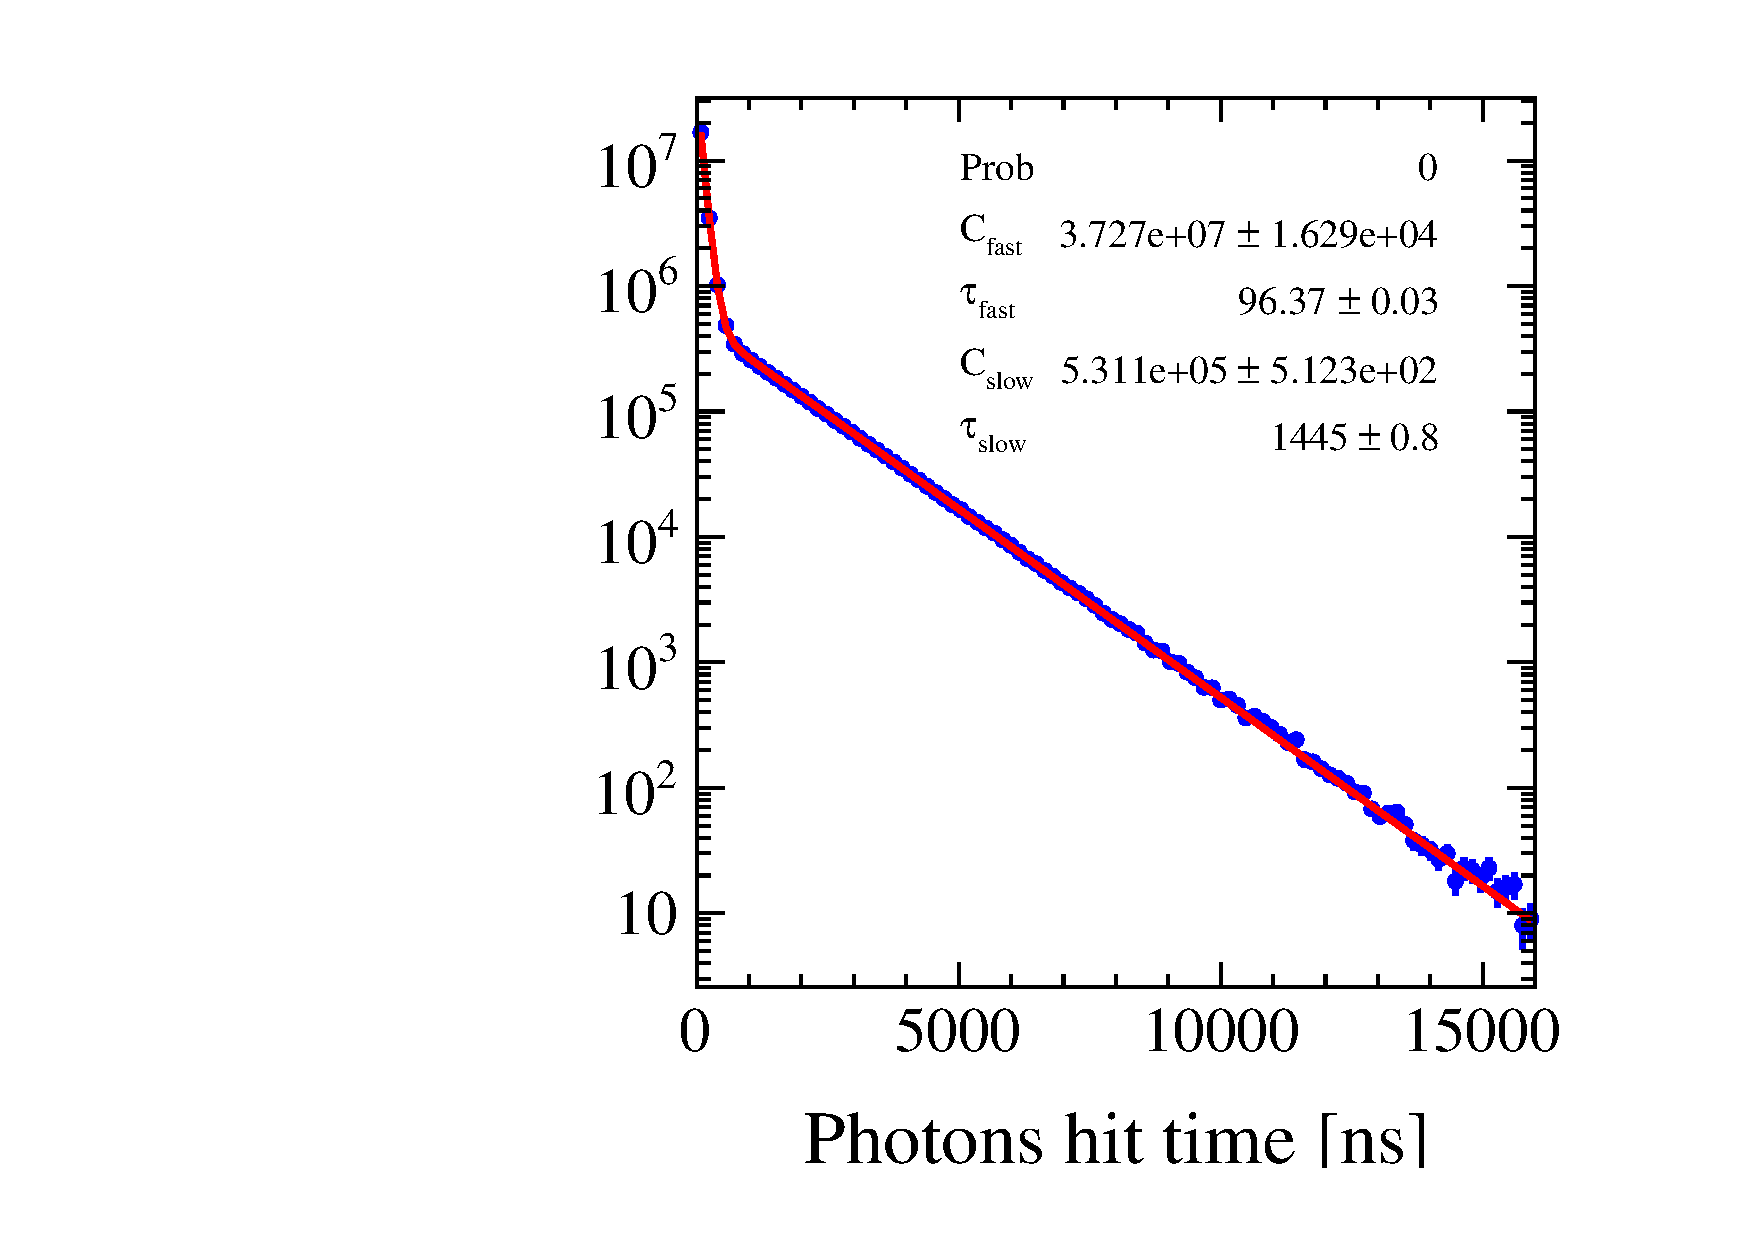
\includegraphics[width=\linewidth]{timeSpe.pdf}
  \caption{}
\end{subfigure}\hfill
\begin{subfigure}{0.38\textwidth}
  \centering
  \includegraphics[width=\linewidth]{Edp.pdf}
  \caption{}
\end{subfigure}
\caption{Simulation validation: (a)~scintillation-time distribution
(fast and slow components); (b)~muon deposited energy in a
\SI{10}{mm}-thick GS cell.}
\label{fig:SiPM_SimValid}
\end{figure}

%% ====================================================================
\section{Experimental characterisation of the baseline active unit}
\label{sec:expchar}
%% ====================================================================

The experimental evidence supporting the baseline active unit spans
four complementary measurement types.
The intrinsic light yield and optical response of the GFO glass
establish its suitability as the active medium.
Radiation-tolerance measurements confirm adequate performance under
CEPC-relevant doses.
Single-cell measurements with three independent probes---a
$^{137}$Cs source, cosmic-ray muons, and \SI{5}{GeV} electrons at
KEK---characterise the cell-level signal across the dynamic range of
interest.
Finally, initial tile-production studies address reproducibility and
quality control at batch scale.

%% --------------------------------------------------------------------
\subsection{Light yield and optical response}
\label{subsec:lightyield}
%% --------------------------------------------------------------------

Figure~\ref{fig:LargeGS} shows GFO glass cells of \cellsize under
natural and ultraviolet illumination.
Figure~\ref{fig:GS40}(a) shows the X-ray-excited luminescence (XEL)
and optical-transmission spectra of the GFO glass; the transmittance
in the visible range exceeds 80\%, with self-absorption observed near
the \SI{400}{nm} emission peak~\cite{SUI2025100878}.
Extensive $\gamma$-ray testing confirms that the GFO intrinsic light
yield consistently exceeds \SI{1000}{\phMeV}.
When measured with an XP2020 \SI{2}{inch} PMT, the GFO
photoelectron yield reaches approximately one-third that of BGO
crystals of identical dimensions~\cite{GS-5}
(Figure~\ref{fig:GS40}b).
Figure~\ref{fig:GS40}(c) shows the scintillation-decay profile under
$\gamma$-ray excitation: the slow-component decay time is below
\SI{500}{ns}, fully compatible with the high granularity and trigger
rate envisaged for the GS-HCAL.

Together these results establish the optical response required to
support the baseline cell: a light yield sufficient for
${\sim}60$~\peMIP readout, a transmittance compatible with bulk
photon transport across the cell, and a decay time compatible with
the baseline trigger window.

\begin{figure}[htbp]
\centering
\begin{subfigure}{0.40\textwidth}
  \centering
  \includegraphics[width=\linewidth]{GSN.pdf}
  \caption{}
\end{subfigure}\hfill
\begin{subfigure}{0.42\textwidth}
  \centering
  \includegraphics[width=\linewidth]{GSUV.pdf}
  \caption{}
\end{subfigure}
\caption{GFO glass cells of \cellsize under (a)~natural light and
(b)~ultraviolet illumination.}
\label{fig:LargeGS}
\end{figure}

\begin{figure}[htbp]
\centering
\begin{subfigure}{0.50\textwidth}
  \centering
  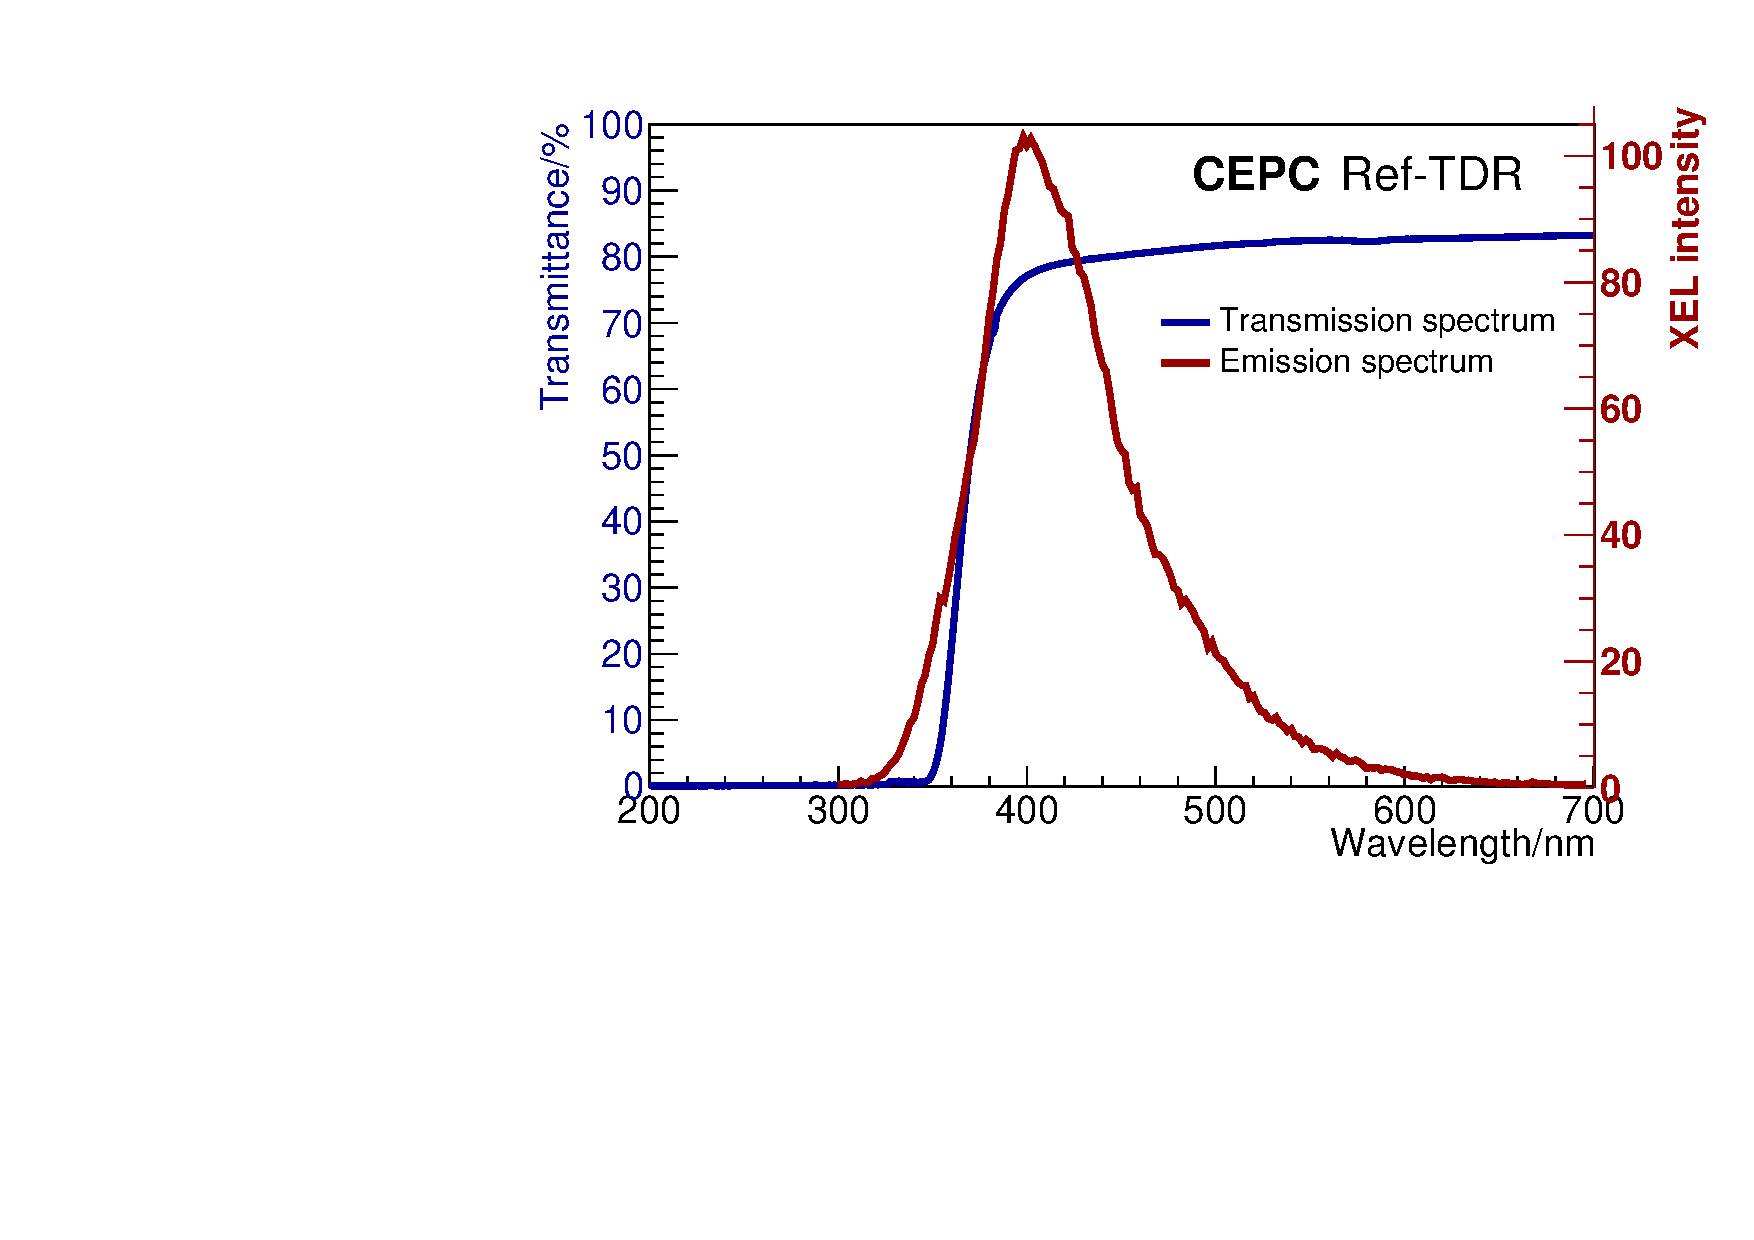
\includegraphics[width=\linewidth]{newGS40-A.pdf}
  \caption{}
  \label{fig:GS40-a}
\end{subfigure}

\vspace{0.3cm}

\begin{subfigure}{0.45\textwidth}
  \centering
  \includegraphics[width=\linewidth]{GS40-b.pdf}
  \caption{}
  \label{fig:GS40-b}
\end{subfigure}\hfill
\begin{subfigure}{0.45\textwidth}
  \centering
  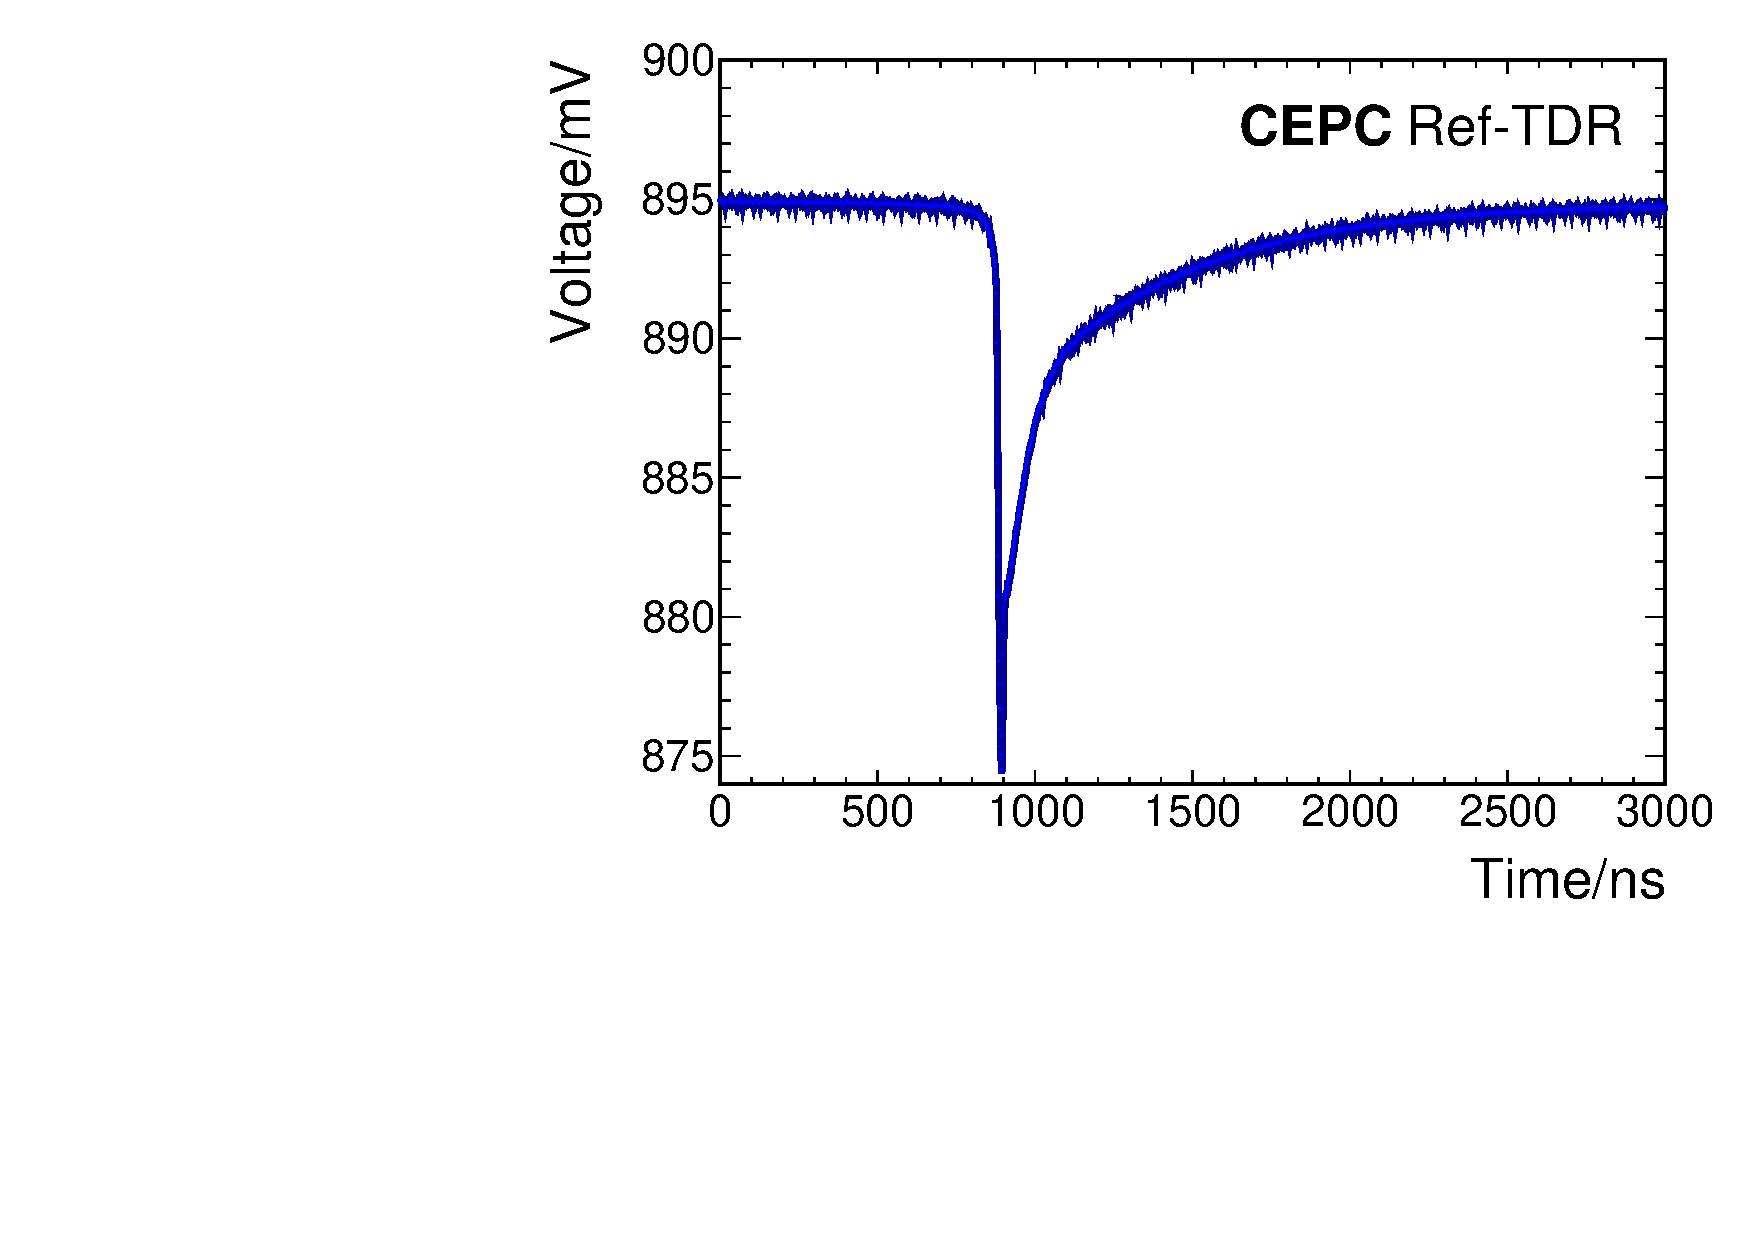
\includegraphics[width=\linewidth]{GS40-c.pdf}
  \caption{}
  \label{fig:GS40-c}
\end{subfigure}
\caption{(a)~Optical-transmission and XEL spectra of the GFO glass.
(b)~Energy spectra of GFO GS and BGO crystal of the same dimensions.
(c)~Scintillation decay curve of the GFO glass.}
\label{fig:GS40}
\end{figure}

%% --------------------------------------------------------------------
\subsection{Radiation tolerance under CEPC-relevant doses}
\label{subsec:radiation}
%% --------------------------------------------------------------------

Under the current CEPC operating plan, the accumulated radiation dose
reaches approximately \SI{40}{Gy} during the ten-year Higgs run at
$\mathcal{L}=8\times10^{34}$~cm$^{-2}$s$^{-1}$, and is estimated at
\SI{96}{Gy} per year during $Z$-pole operation at
$\mathcal{L}=192\times10^{34}$~cm$^{-2}$s$^{-1}$.
A dose benchmark of \SI{100}{Gy} therefore covers the practically
relevant operational range.

Figure~\ref{fig:gamma-irradiation} shows the relative light yield of
GFO glass as a function of $\gamma$-irradiation dose.
The retention exceeds 70\% at \SI{100}{Gy} (measured 71.2\%), and the
result is confirmed by proton-beam irradiation~\cite{YIN2026170869} at
the APEP facility~\cite{Liu:2022czi}.
These measurements demonstrate that the baseline active medium
preserves adequate optical response under CEPC-relevant doses.

\begin{figure}[htbp]
\centering
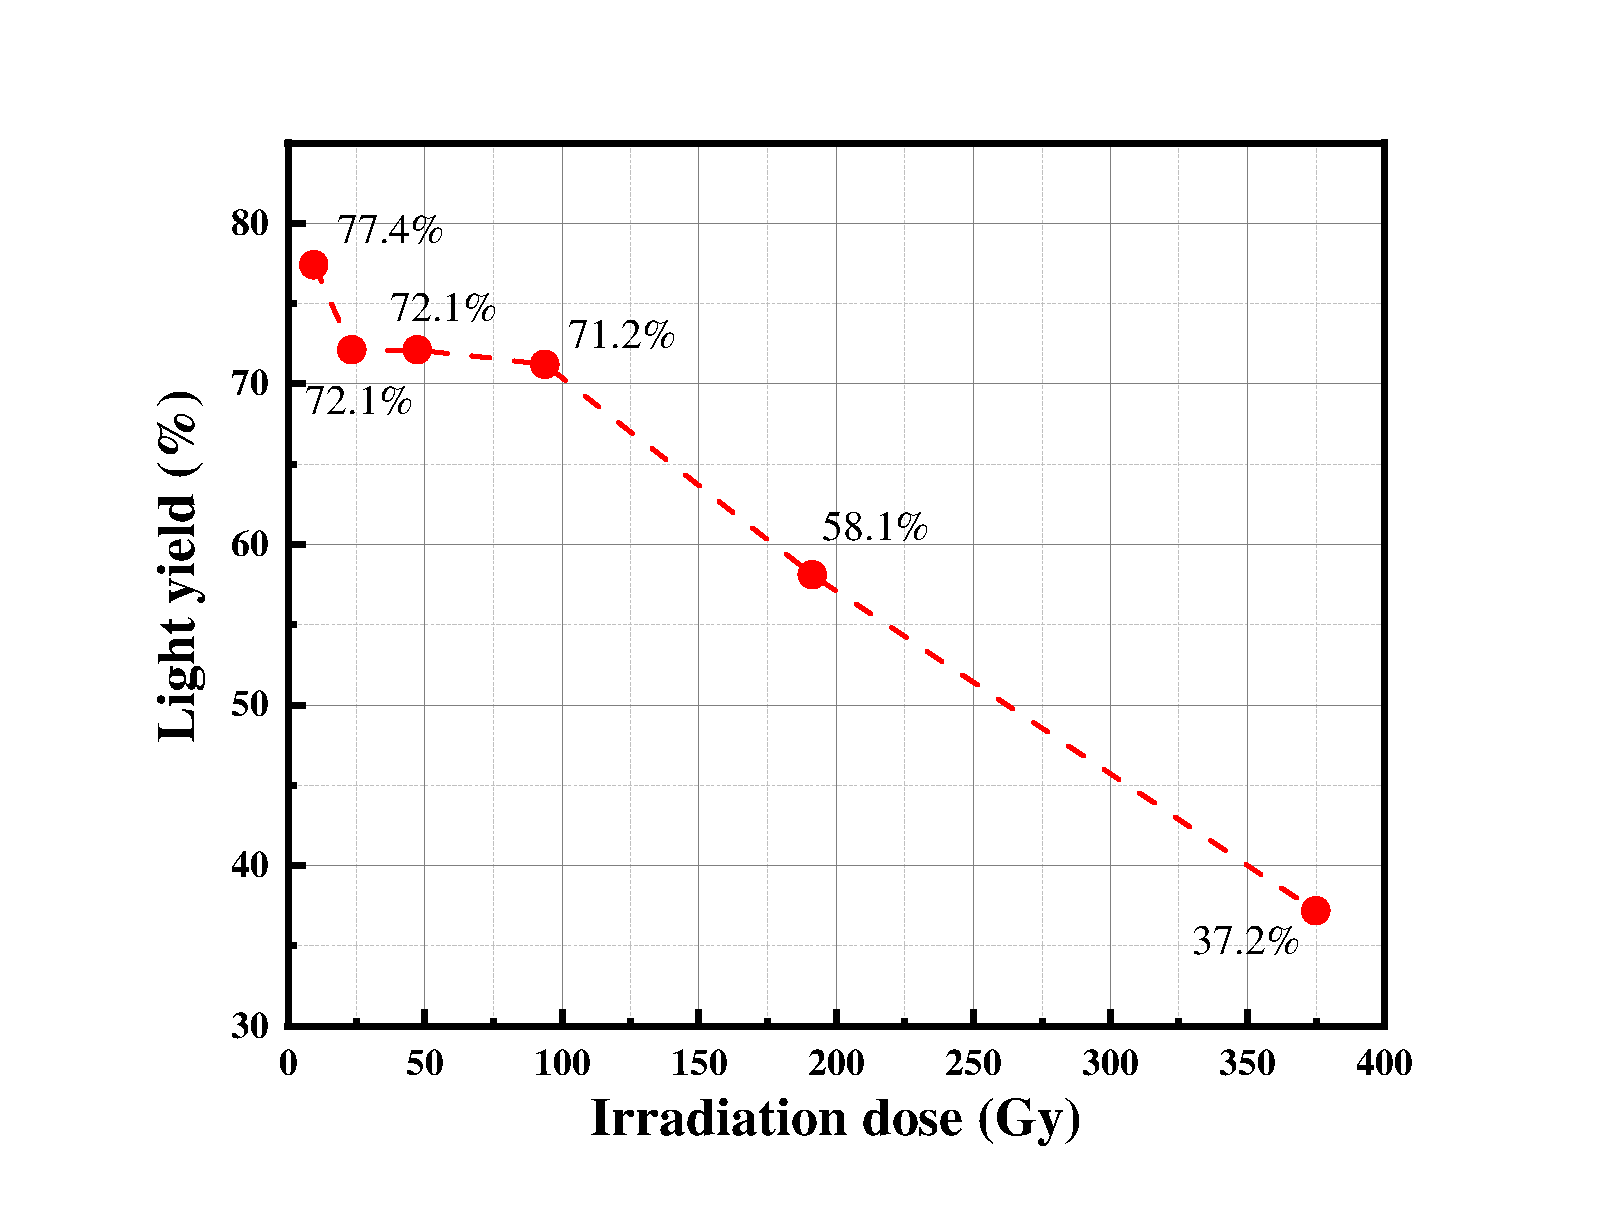
\includegraphics[width=0.60\linewidth]{LightYieldReductionGammaIrradiation.pdf}
\caption{Relative light yield of GFO glass as a function of
$\gamma$-irradiation dose.  At \SI{100}{Gy} the retention is 71.2\%.}
\label{fig:gamma-irradiation}
\end{figure}

%% --------------------------------------------------------------------
\subsection{Single-cell measurements with different probes}
\label{subsec:cellmeas}
%% --------------------------------------------------------------------

The effective light output of the \cellsize GS cell was evaluated in
three independent single-cell measurement campaigns using different
probes:
(i)~\SI{662}{keV} $\gamma$-rays from a $^{137}$Cs source;
(ii)~cosmic-ray muons with an expected energy deposition of
  \SI{7.7}{MeV/MIP};
(iii)~\SI{5}{GeV} electron beams at KEK.
In each case the SiPM was mounted at the cell centre on a readout
board with the interim pre-amplifier of Section~\ref{subsec:fee}.
Comparative tests of enhanced-specular-reflector (ESR) and Teflon
reflective films showed that Teflon provides approximately 20\%
higher effective reflectivity~\cite{Janecek:2012qit}, and all
measurements therefore employ Teflon wrapping.

\paragraph{$^{137}$Cs source.}
Using the HPK~S14160-3050HS SiPM (spectrum-weighted PDE~44.5\%), the
MPV for \SI{662}{keV} $\gamma$-rays is 12.9~p.e.;
scaled to a \SI{7.7}{MeV} MIP energy deposition this corresponds to an
equivalent light output of approximately 150~\peMIP.

\paragraph{Cosmic-ray muons.}
A trigger formed by two plastic-scintillator panels selects
through-going muons.
Using the HPK~S13360-3050PE SiPM (spectrum-weighted PDE~32.5\%), the
measured cell light output is $63.6\pm0.5$~\peMIP
(Figure~\ref{fig:SiPM_Celltest}b).

\paragraph{5~GeV electrons at KEK.}
A Landau fit to the electron spectrum measured with the
NDL~EQR20-11-3030 SiPM (spectrum-weighted PDE~42.5\%) yields an MPV of
$157.6\pm2.9$~\peMIP (Figure~\ref{fig:SiPM_Celltest}c).

\begin{figure}[htbp]
\centering
\begin{subfigure}{0.49\textwidth}
  \centering
  \includegraphics[width=\linewidth]{GS-SiPM-Cs137-Teflon.pdf}
  \caption{}
\end{subfigure}\hfill
\begin{subfigure}{0.49\textwidth}
  \centering
  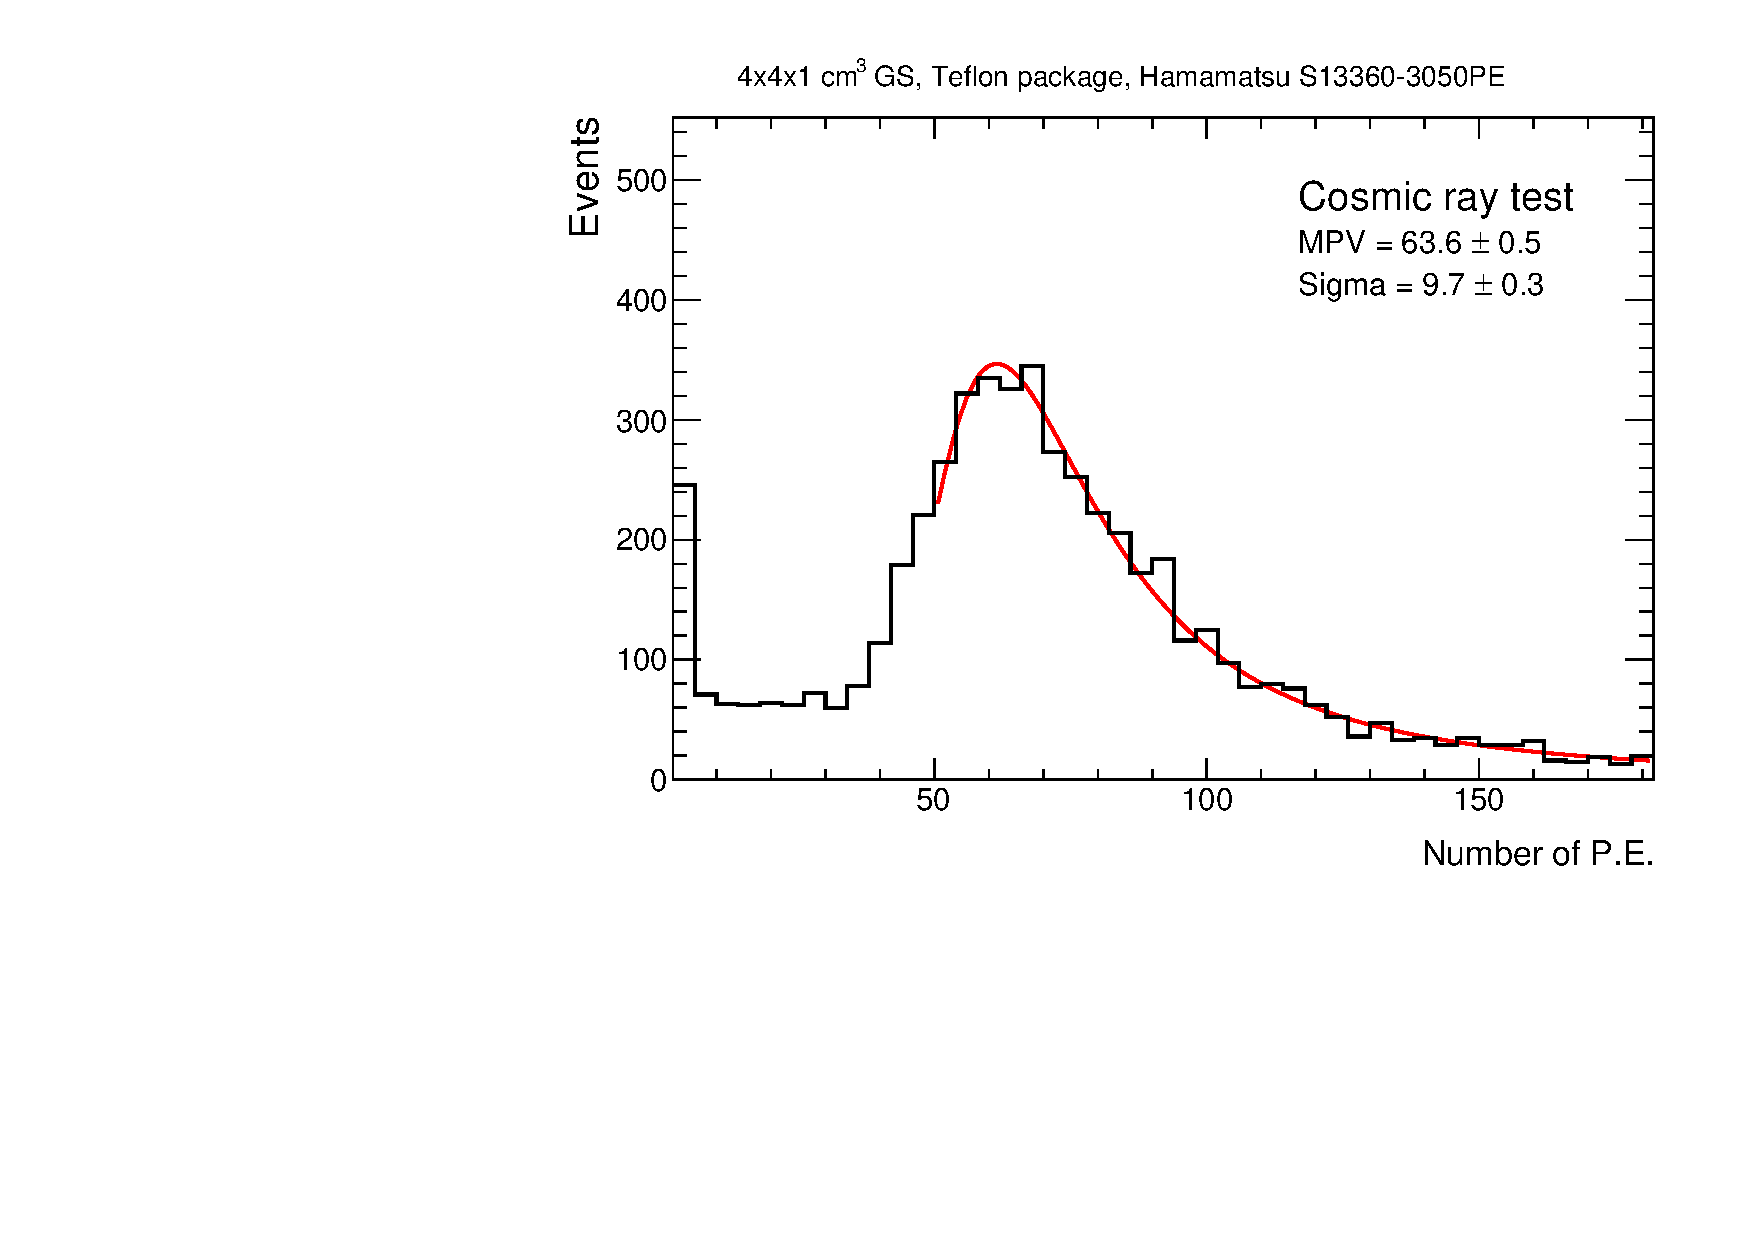
\includegraphics[width=\linewidth]{Cosmic_GSSiPM_SJTU_Teflon.pdf}
  \caption{}
\end{subfigure}

\vspace{0.3cm}

\begin{subfigure}{0.49\textwidth}
  \centering
  \includegraphics[width=\linewidth]{KEK_BeamTest_Electron.png}
  \caption{}
\end{subfigure}
\caption{Single-cell measurement results (\cellsize GS with SiPM
readout).
(a)~ADC spectrum with $^{137}$Cs source (HPK~S14160-3050HS).
(b)~Cosmic-ray test (HPK~S13360-3050PE): $63.6\pm0.5$~\peMIP.
(c)~Response to \SI{5}{GeV} electrons at KEK (NDL~EQR20-11-3030):
Landau-fit MPV $157.6\pm2.9$~\peMIP.}
\label{fig:SiPM_Celltest}
\end{figure}

\paragraph{Interpretation.}
The three probes are complementary rather than directly comparable.
The cosmic-ray muon provides the practical MIP-scale reference
(${\sim}\SI{7.7}{MeV}$ ionisation deposit in \SI{10}{mm} of GFO),
and it is this 64~\peMIP value that enters the baseline digitisation
model (Section~\ref{sec:simperf}).
The \SI{5}{GeV} electron is well above the GFO critical energy
($E_{c}\sim\SI{10}{MeV}$), so it deposits energy through an
electromagnetic shower whose local energy density exceeds that of a
MIP; the resulting 158~\peMIP is therefore higher than the
cosmic-ray value and is not a MIP signal.
The $^{137}$Cs result provides a low-energy check scaled by MIP
equivalence, which is also above the cosmic value.
Taken together the three probes consistently show that the GS cell
plus SiPM provides a signal amplitude well above the threshold
required by the SiPM DCR of Section~\ref{subsec:sipm}, establishing
the practical feasibility of the baseline active unit.
The residual discrepancy with the Geant4 optical simulation
(${\sim}\SI{42}{\peMIP}$) is discussed in
Section~\ref{subsec:optsim}.

%% --------------------------------------------------------------------
\subsection{Reproducibility and quality control}
\label{subsec:qc}
%% --------------------------------------------------------------------

Reproducible tile production is integral to the baseline concept,
because more than five million cells must deliver sufficiently uniform
light yield for PFA reconstruction.
To date approximately 290 tiles of \cellsize have been produced;
about 60\% of them meet the target intrinsic light yield of
\SI{1000}{\phMeV}.
The remaining tile-to-tile variation must be addressed through
two complementary channels: production-side optimisation aiming at a
higher fraction of tiles passing the target, and detector-side
calibration (Section~\ref{subsec:calibration}) that corrects residual
variations through MIP inter-calibration and LED monitoring.
An automated batch-testing platform is being developed to measure
light-yield uniformity, attenuation-length consistency, and
dimensional tolerances across large production batches, and a
production run of approximately \num{10000} tiles is planned to equip
the full-size prototype.
Mass-production optimisation of GFO tile yield and uniformity is
therefore recognised as one of the baseline's open engineering
items.

%% ====================================================================
\section{Simulation framework and projected detector performance}
\label{sec:simperf}
%% ====================================================================

The projected performance of the baseline detector is obtained from
full Geant4 digitisation-based simulation of the baseline geometry
within the CEPCSW framework.
These results are type-B evidence in the classification of
Section~\ref{subsec:why-baseline}: they establish that the baseline
configuration is consistent with the CEPC performance goals under the
current modelling assumptions, before full prototype beam validation.

%% --------------------------------------------------------------------
\subsection{Simulation setup and digitisation assumptions}
\label{subsec:simsetup}
%% --------------------------------------------------------------------

The simulation is performed with Geant4 within the CEPCSW
framework~\cite{CEPCStudyGroup:2018ghi}.
For single-hadron studies all inner sub-detectors are removed so that
the intrinsic GS-HCAL response is isolated; for physics-benchmark
studies the full reference-detector setup is used.
The digitisation model implements the following current modelling
assumptions:

\begin{itemize}
\item \textbf{Birks' constant:} a preliminary value
  $k_{B}=\SI{0.01}{cm/MeV}$, pending a dedicated heavy-ion
  measurement.
\item \textbf{Intrinsic light yield:} \SI{1500}{\phMeV}, giving a
  detected effective single-cell output of $\geq60$~\peMIP.
\item \textbf{Light attenuation length:} \SI{6}{cm}, taken from the
  current transmittance measurement.
\item \textbf{Readout threshold:} \SI{0.1}{MIP}, selected from a
  dedicated scan of its impact on the energy resolution.
\item \textbf{SiPM response and electronics effects:} included with
  the candidate SiPM parameters of Table~\ref{tab:SiPM-tab1}.
\end{itemize}

These are \emph{current modelling assumptions}: they are grounded in
measurements, but a subset of them (notably the Birks constant and
the optical-simulation light yield) is known to require further
tuning, and full experimental closure of the simulation chain is one
of the objectives of the prototype beam-test programme.

%% --------------------------------------------------------------------
\subsection{Single-hadron energy response}
\label{subsec:hadronres}
%% --------------------------------------------------------------------

The single-hadron energy resolution of the GS-HCAL is parametrised as
\begin{equation}
\label{eq:eres}
\frac{\sigma_{E}}{E} = \frac{a}{\sqrt{E}} \oplus b,
\end{equation}
where $a$ is the stochastic term and $b$ the constant term.
With the present digitisation model, and before full prototype beam
validation, the baseline detector configuration predicts
\begin{equation}
\frac{\sigma_{E}}{E} = \frac{29.8\%}{\sqrt{E\,[\text{GeV}]}}
\oplus 6.5\%,
\end{equation}
with energy non-linearity within 2\% (Figure~\ref{fig:Eres_HCAL_final};
\texttt{QGSP\_BERT} hadronic physics list).
The stochastic term is substantially below that of conventional
sampling HCALs (${\sim}60\%/\sqrt{E}\oplus3\%$), reflecting the high
active-medium density of the baseline.
The constant term is larger than the final CEPC target and is
dominated by longitudinal leakage in the $6\,\lambdaI$ design; this is
analysed in Section~\ref{subsec:constterm}.

\begin{figure}[htbp]
\centering
\begin{subfigure}{0.45\linewidth}
  \centering
  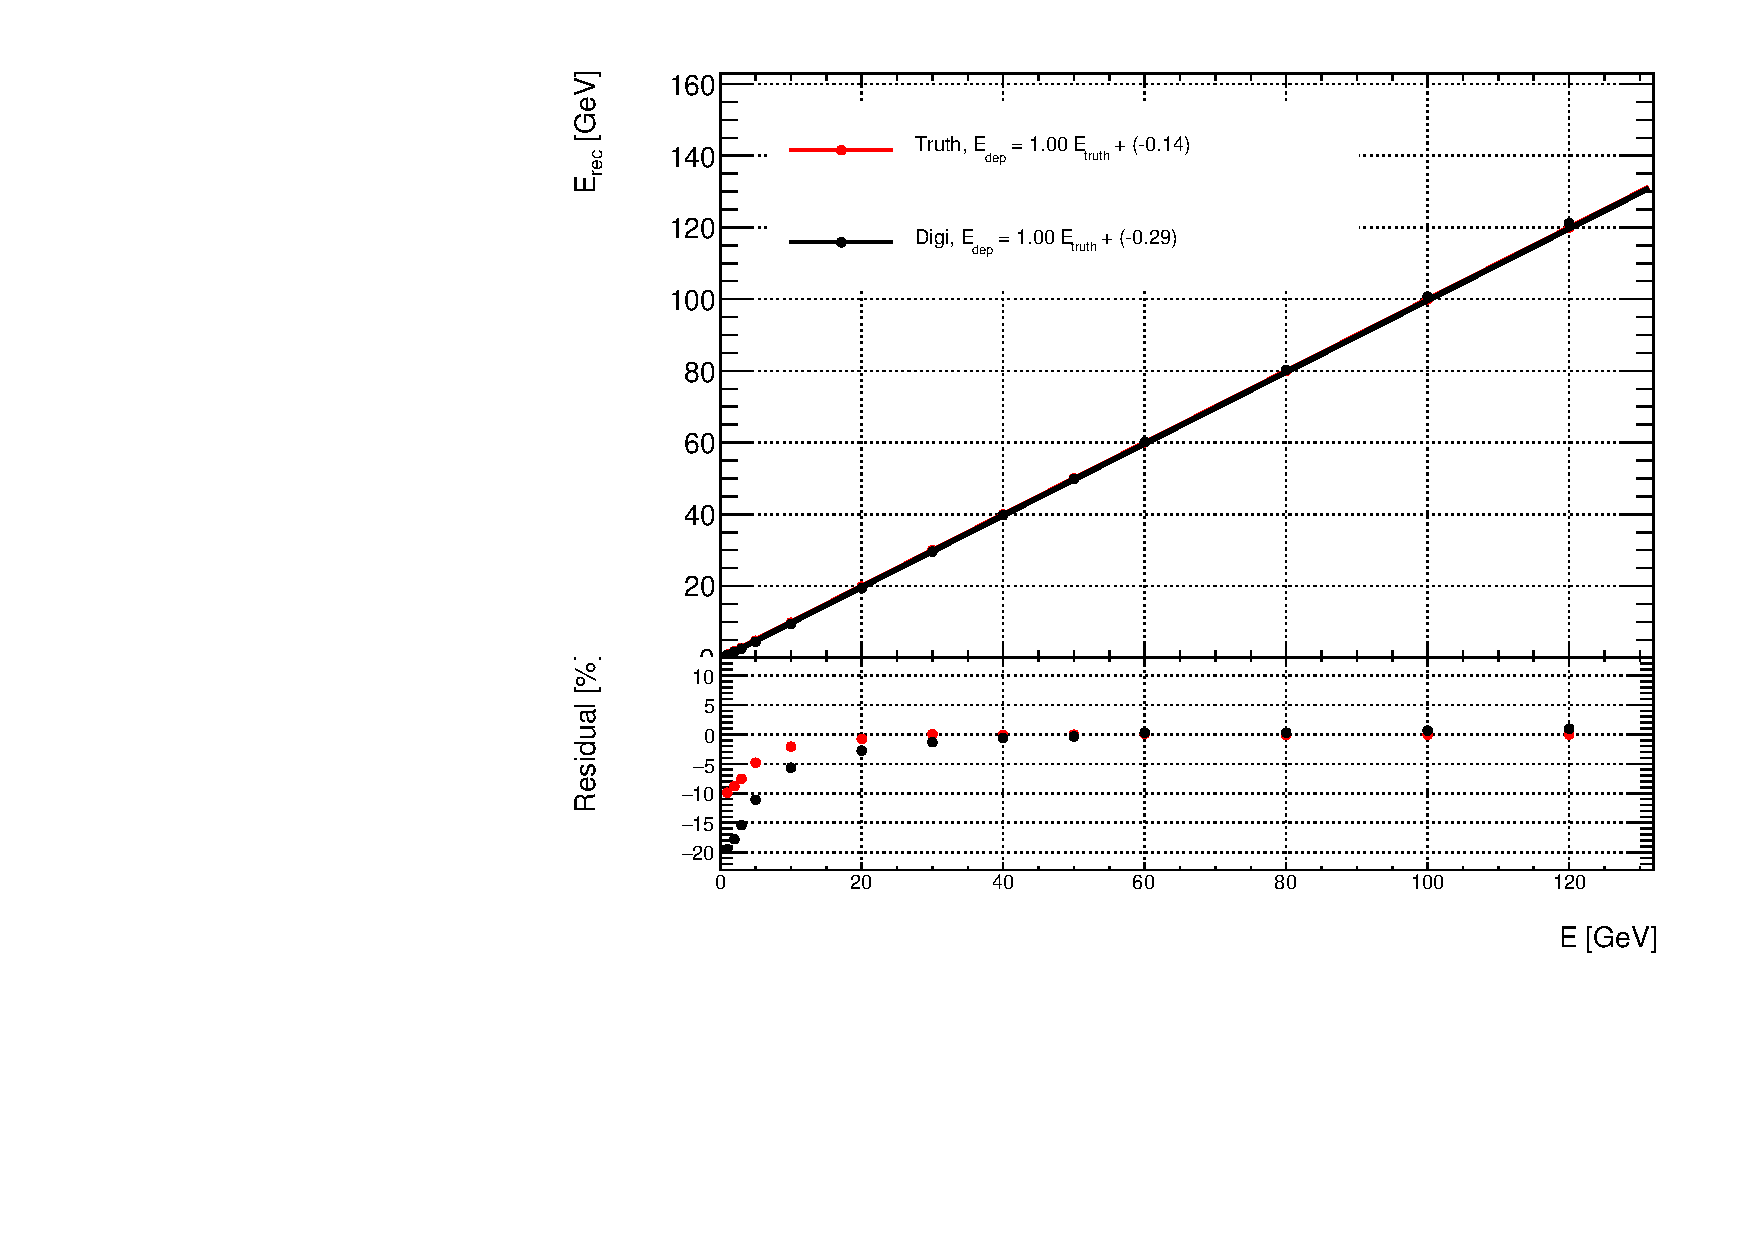
\includegraphics[width=\linewidth]{Elin_digi.pdf}
  \caption{}
\end{subfigure}\hfill
\begin{subfigure}{0.45\linewidth}
  \centering
  \includegraphics[width=\linewidth]{Eres_digi.pdf}
  \caption{}
\end{subfigure}
\caption{(a)~Energy linearity and (b)~energy resolution of the
baseline GS-HCAL from the full digitisation model.}
\label{fig:Eres_HCAL_final}
\end{figure}

In the CEPC collision environment
(Figure~\ref{fig:Ehad_CEPC}), more than 98\% of hadronic final-state
objects have energies below \SI{60}{GeV}, which is precisely the
regime in which the GS-HCAL stochastic term dominates and the
predicted resolution is best.

\begin{figure}[htbp]
\centering
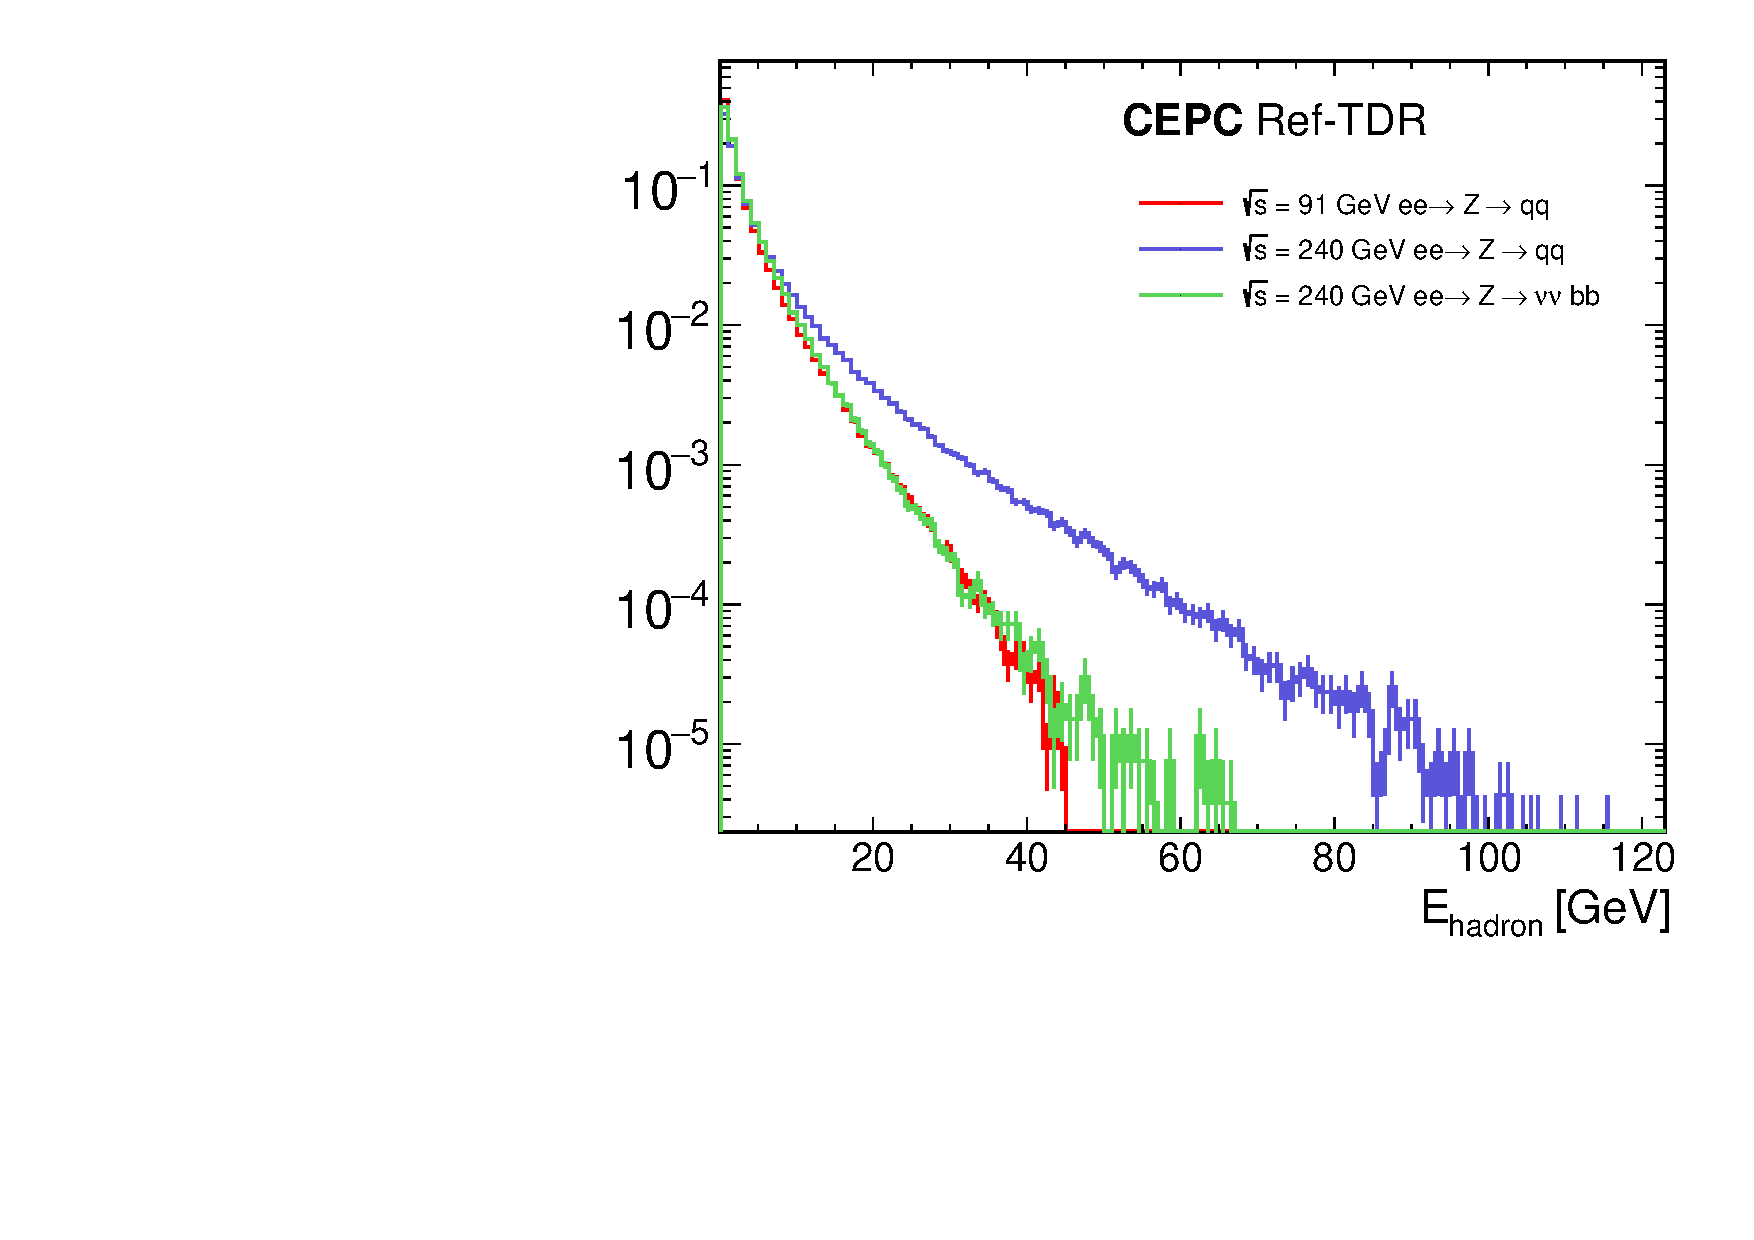
\includegraphics[width=0.50\linewidth]{Ehadrons.pdf}
\caption{Energy distribution of hadronic final-state objects in the
most energetic CEPC $e^{+}e^{-}$ processes.}
\label{fig:Ehad_CEPC}
\end{figure}

%% --------------------------------------------------------------------
\subsection{Sensitivity to key detector parameters}
\label{subsec:sensitivity}
%% --------------------------------------------------------------------

The sensitivity of the predicted single-hadron resolution to the
principal digitisation parameters is shown in
Figure~\ref{fig:Eres_vs_parameters} for
(a)~light output and readout threshold, (b)~attenuation length, and
(c)~Birks' constant.
These scans are not auxiliary: they are evidence that the baseline
parameter choices sit in a stable region of the resolution landscape.
In particular, the achieved cosmic-ray light output of
${\sim}\SI{64}{\peMIP}$ is well inside the saturated region of the
light-output/threshold scan, and the measured attenuation length of
${\sim}\SI{6}{cm}$ is likewise in the plateau of curve~(b).
The Birks-constant dependence quantifies the residual sensitivity
that will be reduced once a dedicated measurement is available.

\begin{figure}[htbp]
\centering
\begin{subfigure}{0.48\linewidth}
  \centering
  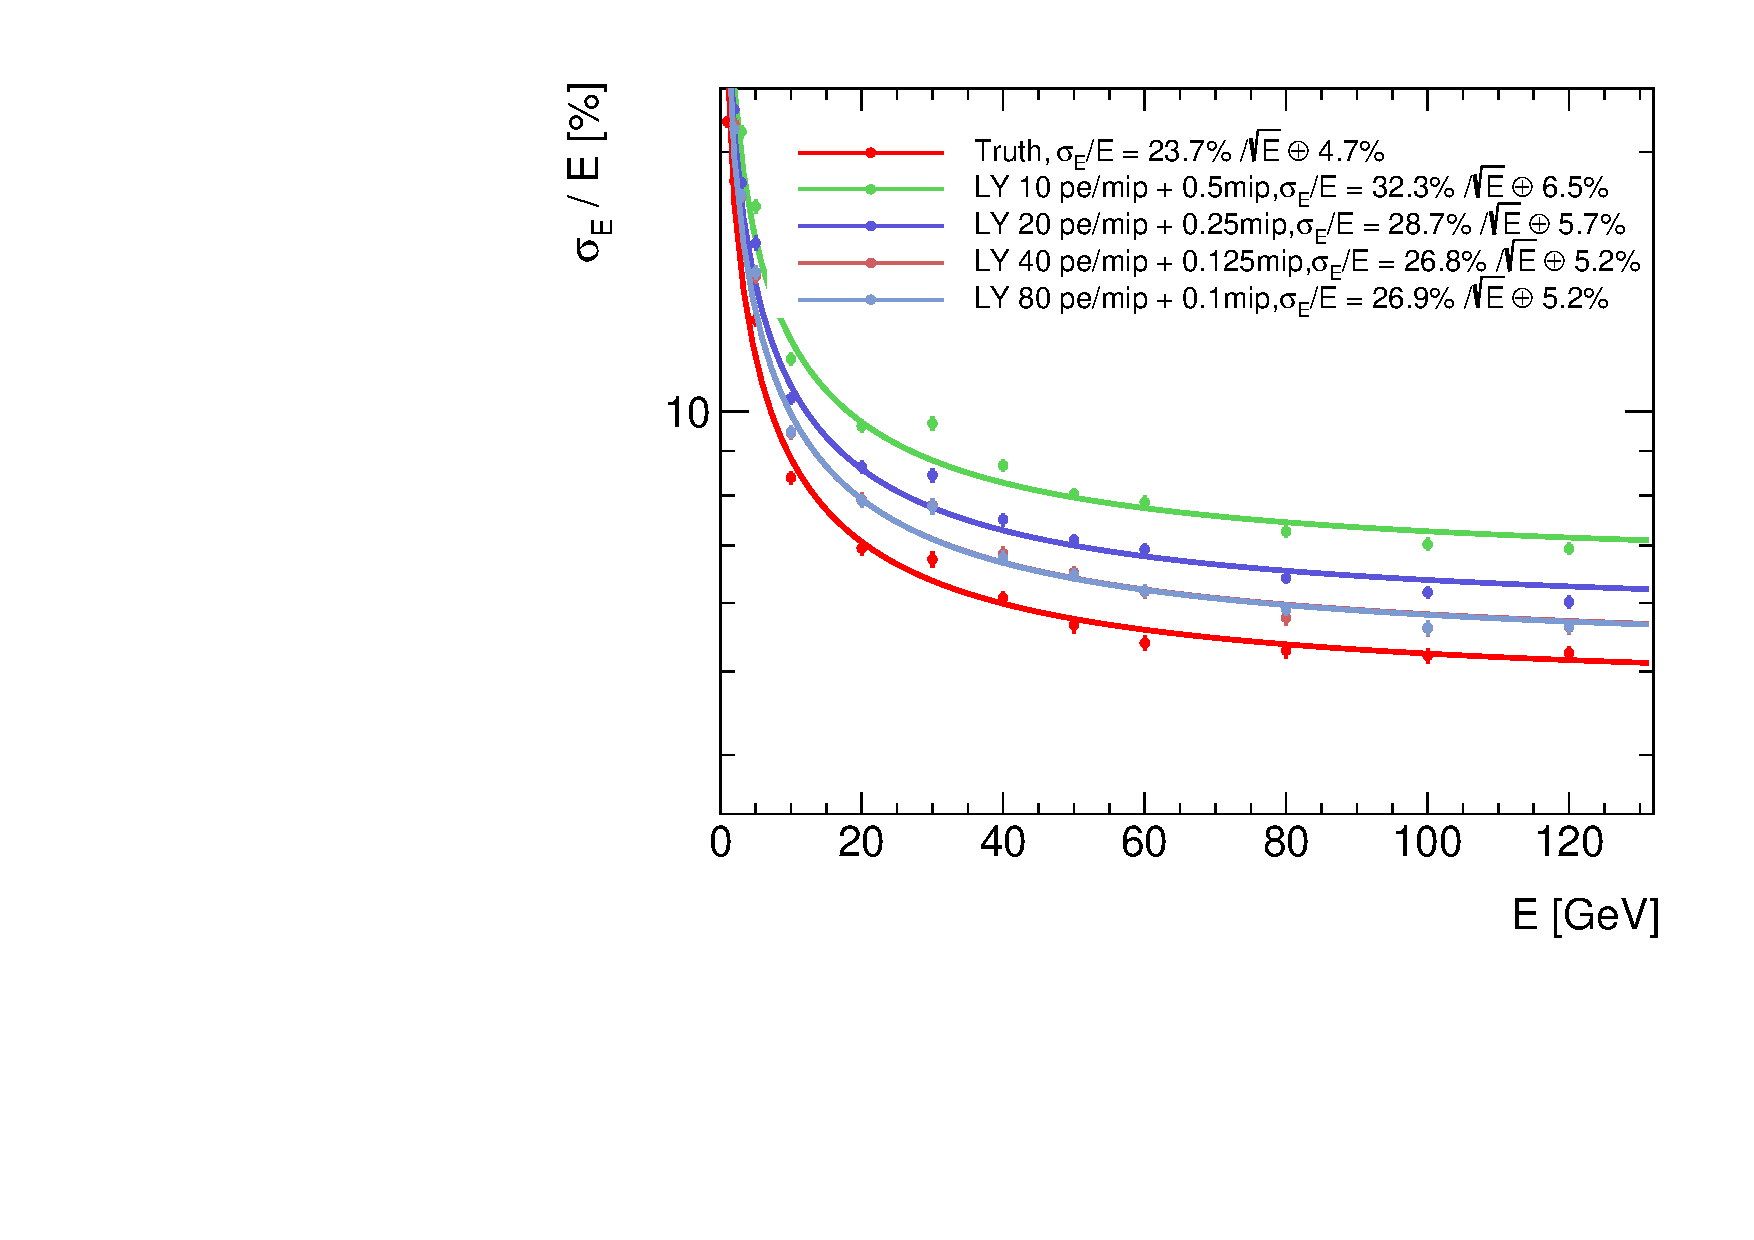
\includegraphics[width=\linewidth]{Eres_LYTh_Log.pdf}
  \caption{}
\end{subfigure}\hfill
\begin{subfigure}{0.48\linewidth}
  \centering
  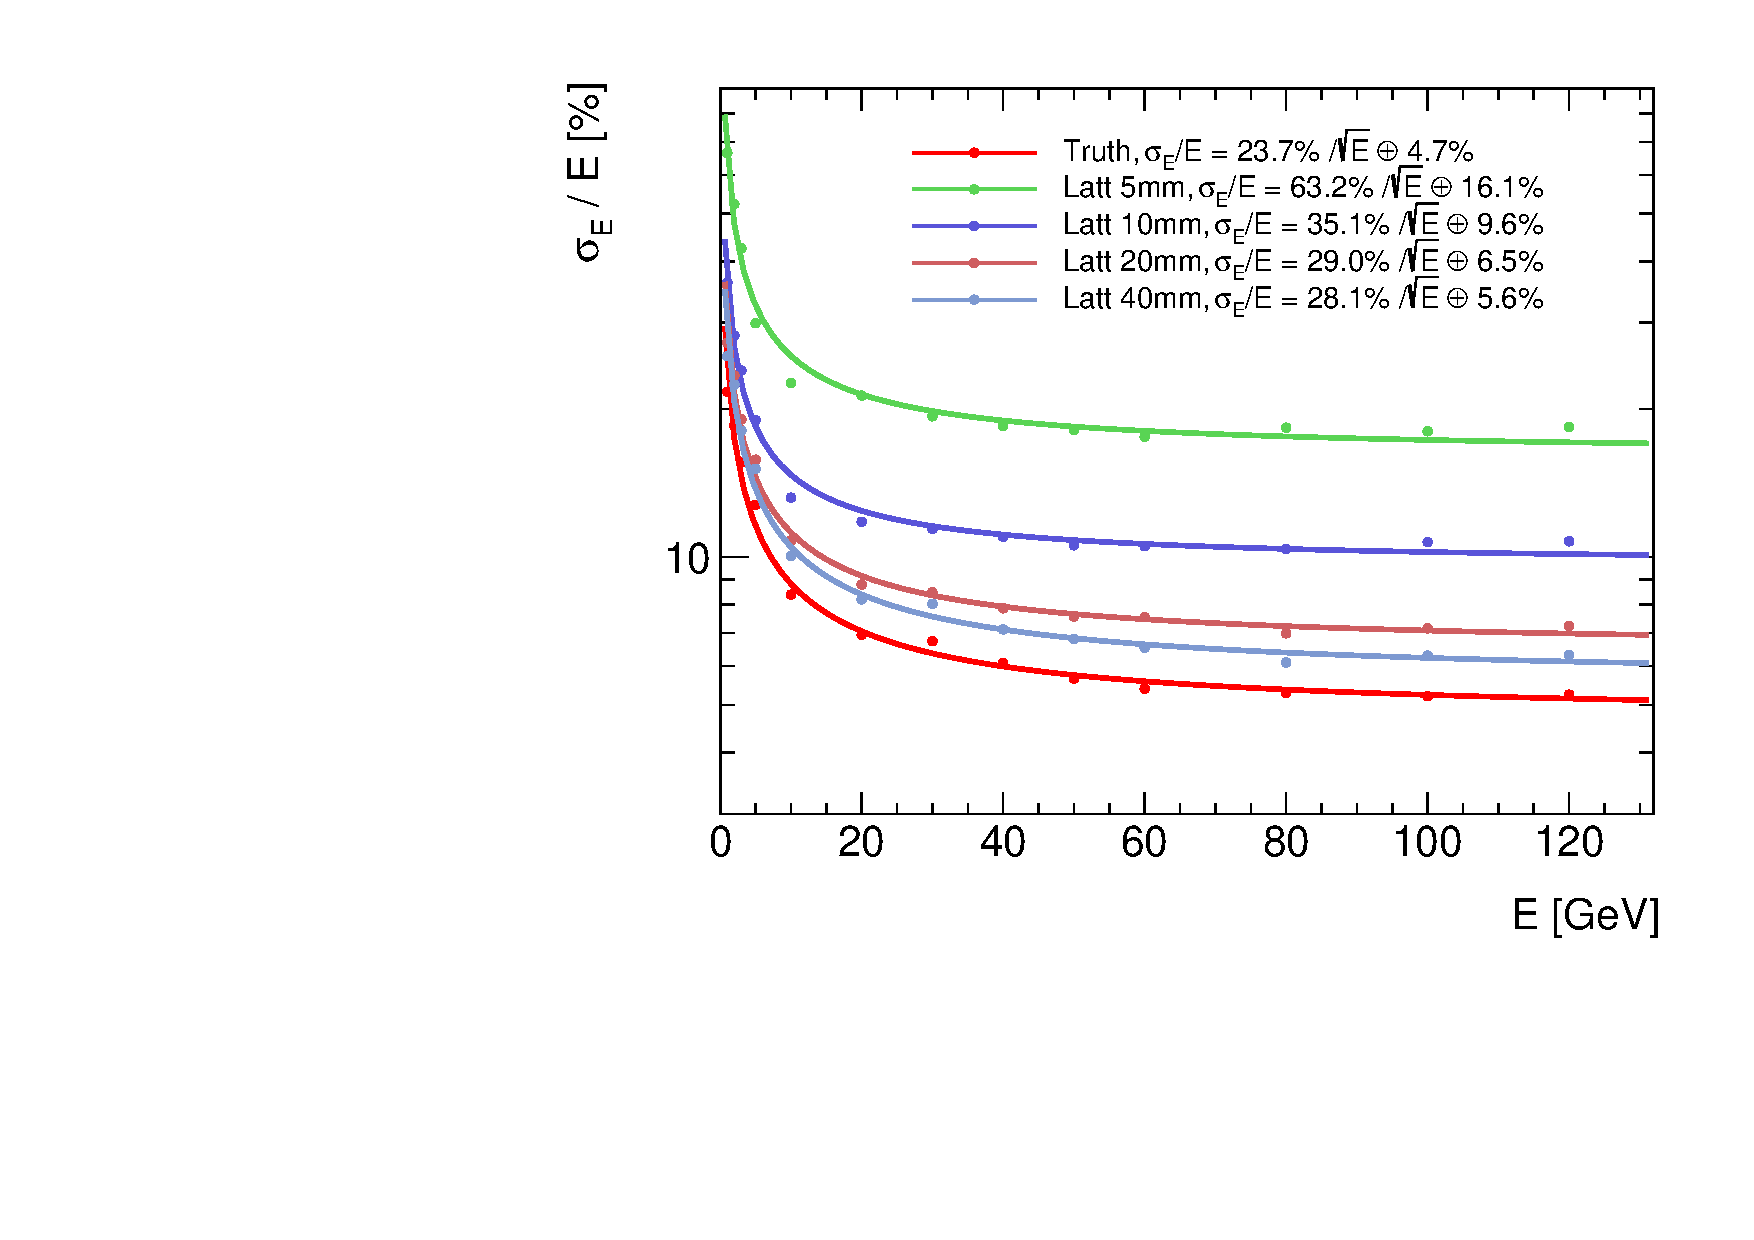
\includegraphics[width=\linewidth]{Eres_Latt_log.pdf}
  \caption{}
\end{subfigure}

\vspace{0.3cm}

\begin{subfigure}{0.48\linewidth}
  \centering
  \includegraphics[width=\linewidth]{ERes_Birks.pdf}
  \caption{}
\end{subfigure}
\caption{Simulated energy resolution as a function of
(a)~light output and readout threshold,
(b)~GS attenuation length, and
(c)~Birks' constant.}
\label{fig:Eres_vs_parameters}
\end{figure}

%% --------------------------------------------------------------------
\subsection{Origin of the constant term}
\label{subsec:constterm}
%% --------------------------------------------------------------------

The 6.5\% constant term obtained in Section~\ref{subsec:hadronres} is
interpreted as being dominated by longitudinal leakage in the
$6\,\lambdaI$ design.
Two independent studies support this interpretation.

First, increasing the standalone HCAL depth from 48~layers
($6\,\lambdaI$) to 80~layers ($10\,\lambdaI$) reduces the constant
term from 4.7\% to 2.9\% (Figure~\ref{fig:depth}), confirming that
leakage is the dominant source.

Second, the upstream environment of the full reference detector is
expected to mitigate this effect.
The BGO ECAL contributes ${\approx}1.2\,\lambdaI$ of upstream
material, causing approximately 70\% of hadrons to initiate showers
before entering the HCAL.
Requiring the first hadronic interaction to occur within the first two
GS-HCAL layers ($0.25\,\lambdaI$) already reduces the constant term to
approximately 3\%, consistent with the PS-HCAL prototype
result~\cite{CALICE:2010fpb,Liu:2025hgf}.

This analysis identifies leakage rather than the intrinsic GS-HCAL
response as the origin of the current constant term; it does not
itself close the constant term, but it shows that the baseline
architecture is compatible with the target 3--4\% BMR.

\begin{figure}[htbp]
\centering
\begin{subfigure}{0.48\textwidth}
  \centering
  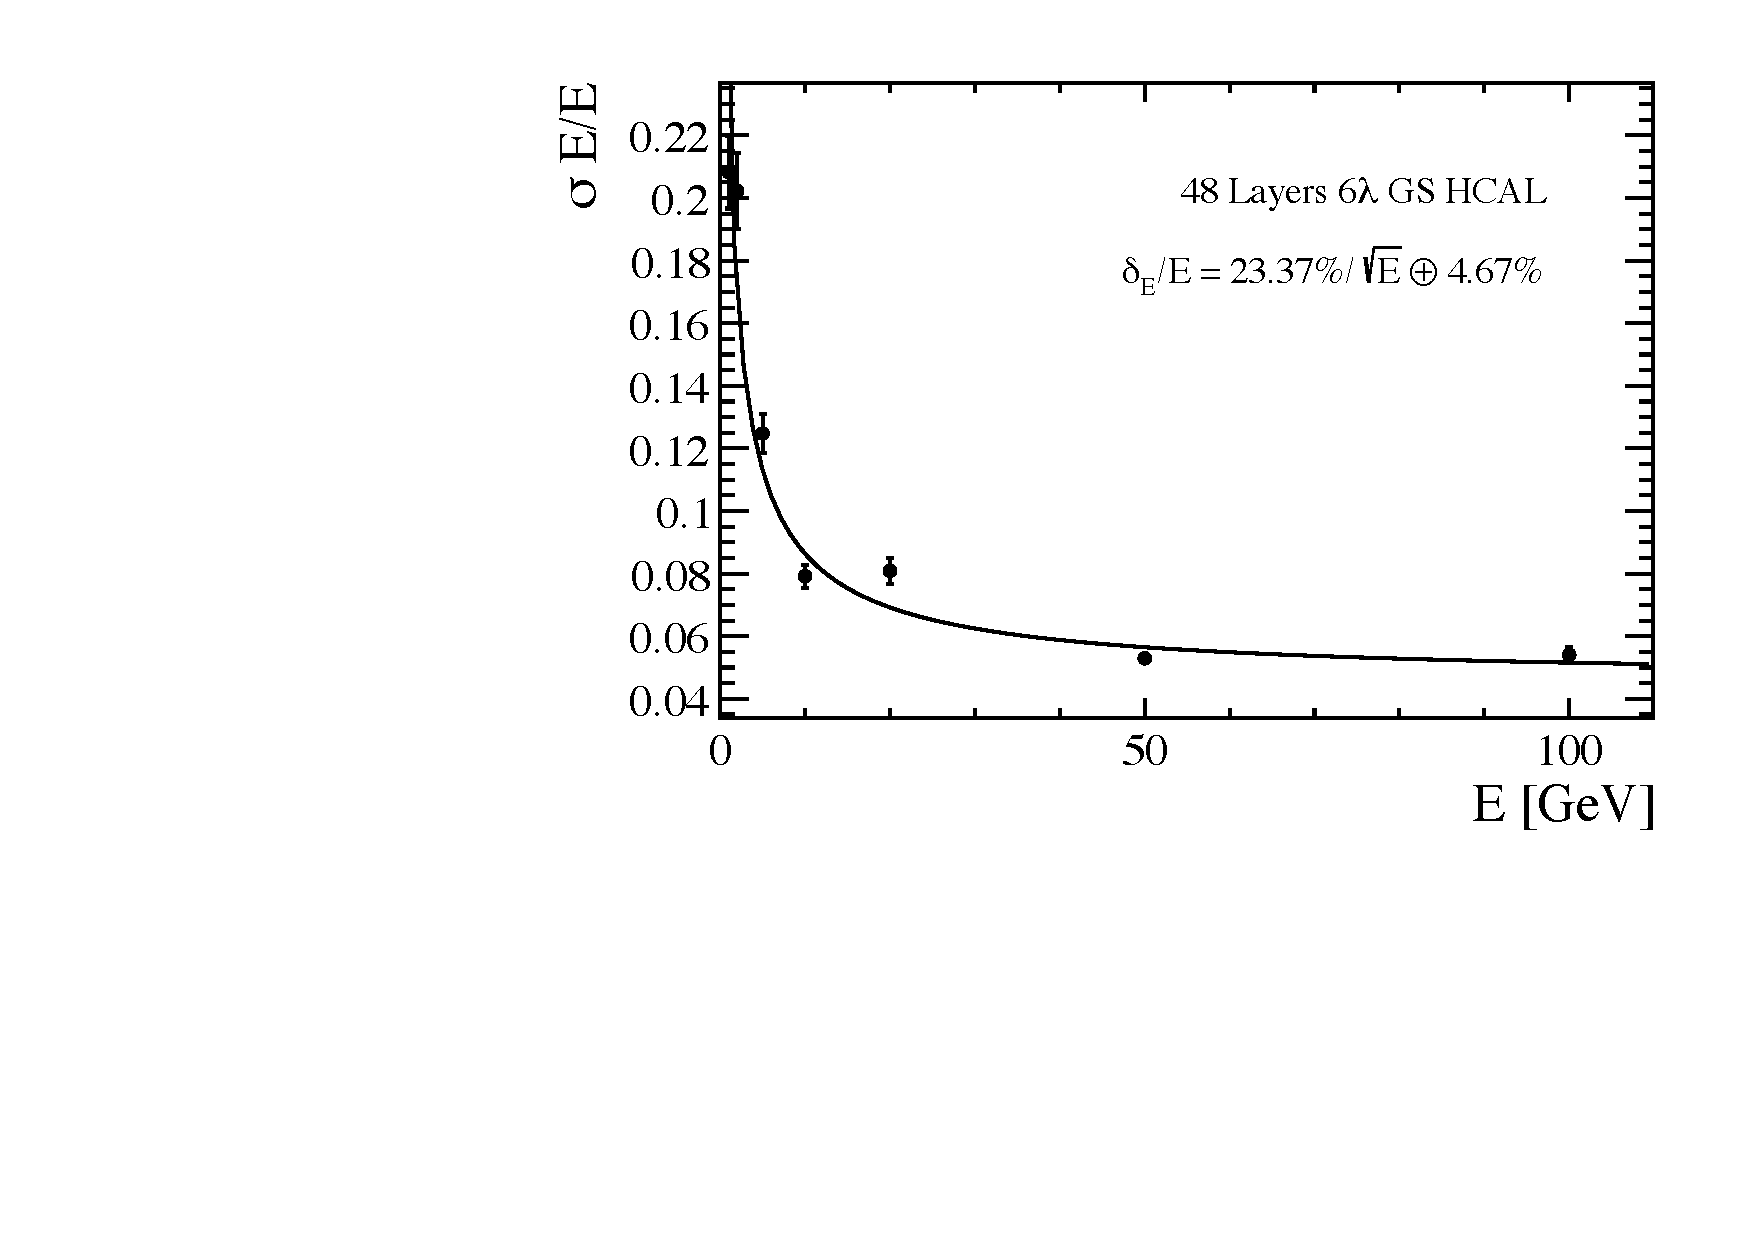
\includegraphics[width=\linewidth]{const_gs_6lambda.pdf}
  \caption{}
\end{subfigure}\hfill
\begin{subfigure}{0.48\textwidth}
  \centering
  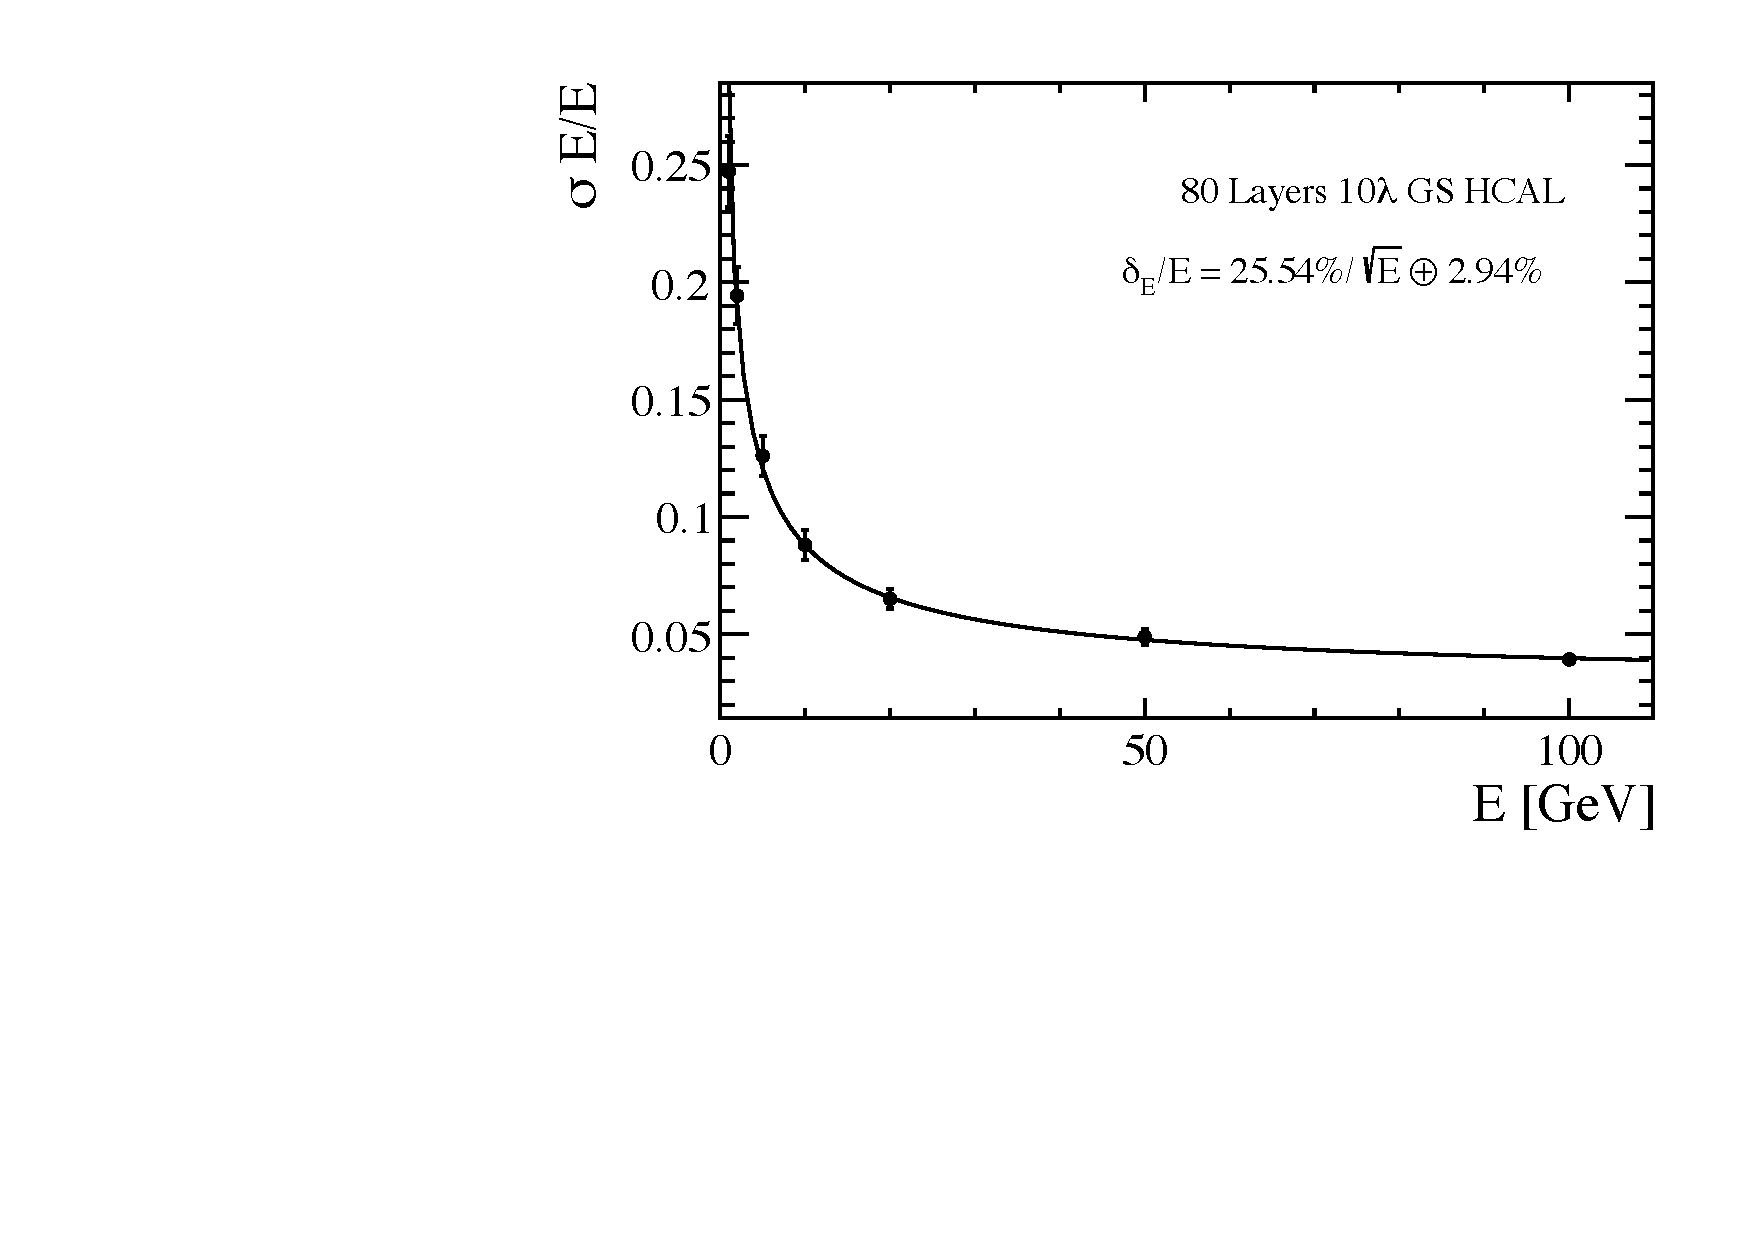
\includegraphics[width=\linewidth]{const_gs_10lambda.pdf}
  \caption{}
\end{subfigure}
\caption{Energy-resolution distributions for two GS-HCAL depths.
(a)~$6\,\lambdaI$ (48~layers): pronounced high-energy tail.
(b)~$10\,\lambdaI$ (80~layers): constant term reduced from 4.7\%
to 2.9\%.}
\label{fig:depth}
\end{figure}

%% --------------------------------------------------------------------
\subsection{Electron--hadron response}
\label{subsec:eresponse}
%% --------------------------------------------------------------------

The baseline calorimeter response to electrons and to different
hadron species is studied with full Geant4 simulation of the
standalone GS-HCAL\@.
Fitting $E_{\mathrm{true}}=C\times S_{\mathrm{HCAL}}$ separately for
each species gives the calibration slopes of
Table~\ref{tab:eoverh_hcal}.
The empirical hadron-to-electron response ratio
$C_{\mathrm{hadron}}/C_{e}$ of 1.09--1.14 is consistent with a
non-compensating sampling calorimeter~\cite{Akchurin:2012zz}.
The empirical ratio must be distinguished from the intrinsic
compensation ratio $e/h$ of the shower physics, which is the actual
figure of merit for the constant term; the intrinsic $e/h$ has not
yet been extracted, and its extraction through shower-component
decomposition is part of the open-item list of
Section~\ref{sec:discussion}.
Software-compensation and energy-weighting techniques
exploiting this intrinsic $e/h$ are expected to reduce the constant
term below~3\%.

\begin{table}[htbp]
\centering
\caption{Calibration slopes $C$ and electron--hadron response ratios
$C_{\mathrm{hadron}}/C_{e}$ for the baseline GS-HCAL\@.}
\label{tab:eoverh_hcal}
\begin{tabular}{lcc}
\toprule
Particle & $C$ (slope) & $C_{\mathrm{hadron}}/C_{e}$ \\
\midrule
Electron  & $2.94\pm0.01$ & ---            \\
$\pi^{-}$ & $3.20\pm0.05$ & $1.09\pm0.02$ \\
$K^{+}$   & $3.28\pm0.05$ & $1.12\pm0.02$ \\
Neutron   & $3.35\pm0.07$ & $1.14\pm0.02$ \\
Proton    & $3.36\pm0.07$ & $1.14\pm0.02$ \\
\bottomrule
\end{tabular}
\end{table}

%% --------------------------------------------------------------------
\subsection{Physics benchmark: $H\to gg$}
\label{subsec:physperf}
%% --------------------------------------------------------------------

The physics-benchmark performance of the baseline is evaluated through
PFA reconstruction of $H\to gg$, the most HCAL-sensitive of the
standard Higgs-dijet benchmarks.
Events are generated with \textsc{Whizard}\,v1.9.5~\cite{Kilian:2007gr,
Moretti:2001zz} and propagated through the full reference-detector
simulation with Geant4\,v11.2 in the CEPCSW framework.
Figure~\ref{fig:ch08_BMR} shows the reconstructed dijet invariant
mass; the fitted Higgs-boson mass is
$126.32\pm0.04$~GeV/$c^{2}$ with
$\sigma(m_{jj})=4.90\pm0.04$~GeV/$c^{2}$, corresponding to a boson
mass resolution (BMR) of 3.88\%, within the CEPC target of 3--4\%.

This result is detector-level strong evidence that the baseline
concept is compatible with the CEPC physics goals, but it is
simulation-based and does not replace prototype beam validation.

\begin{figure}[htbp]
\centering
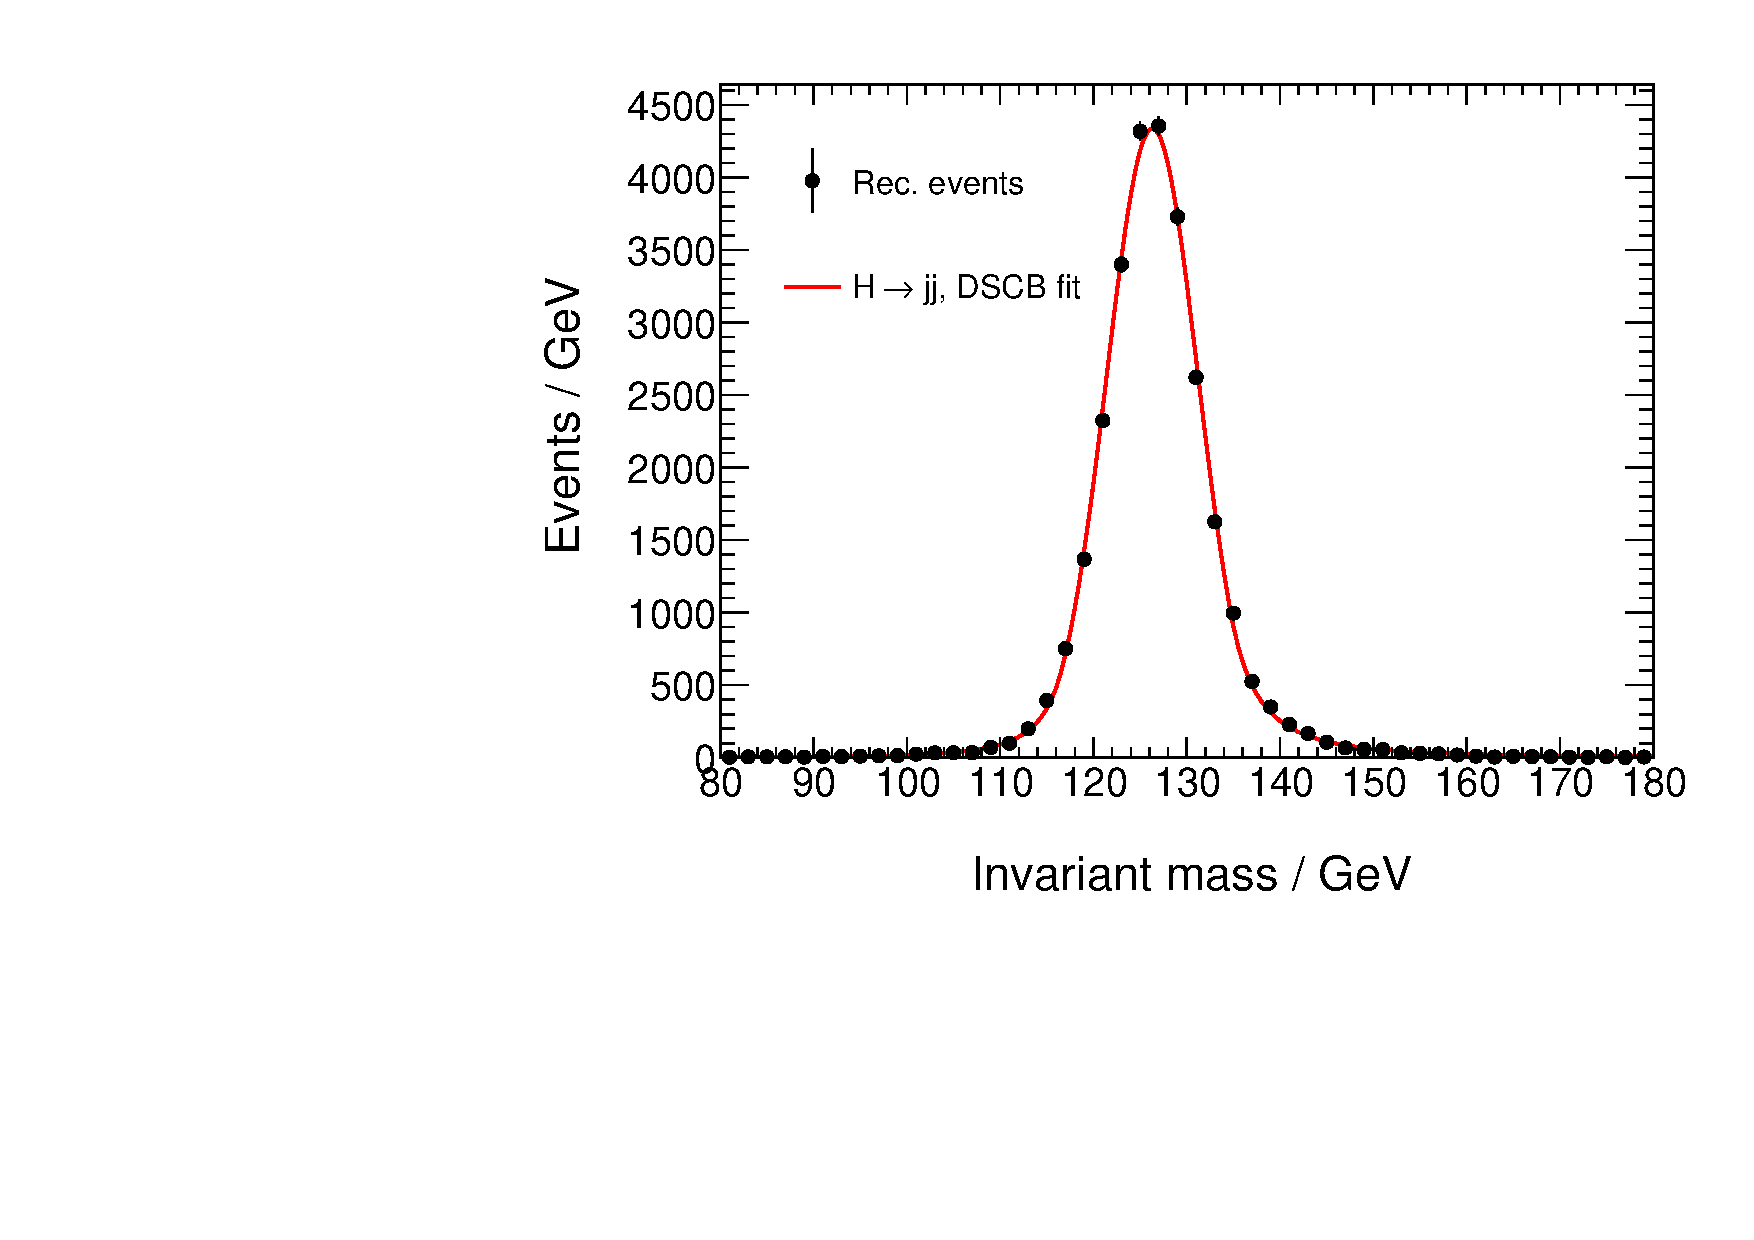
\includegraphics[width=0.60\linewidth]{Fig8.9_BMR.pdf}
\caption{Reconstructed dijet invariant mass for $H\to gg$ with the
baseline GS-HCAL\@.
Fitted mass: $126.32\pm0.04$~GeV/$c^{2}$;
$\sigma(m_{jj})=4.90\pm0.04$~GeV/$c^{2}$; BMR~=~3.88\%.}
\label{fig:ch08_BMR}
\end{figure}

%% ====================================================================
\section{Mechanical feasibility, calibration strategy, and prototype
validation}
\label{sec:feasibility}
%% ====================================================================

Establishing the technical basis of the baseline requires not only
material and simulation evidence but also demonstrated detector-scale
mechanical viability, a defined calibration architecture, and a
concrete prototype beam-test plan.
These three aspects are presented together because they jointly
determine whether the baseline can be realised at full scale.

%% --------------------------------------------------------------------
\subsection{Mechanical feasibility at detector scale}
\label{subsec:mechanics}
%% --------------------------------------------------------------------

Finite-element analysis of the full barrel+endcap structure supports
the detector-scale mechanical viability of the baseline concept.
The critical load is the \SI{135}{t} BGO ECAL supported by the
barrel while the layer-to-layer alignment required by PFA is
preserved.
Figure~\ref{fig:deformation_barrel} shows the deformation distribution
with and without ECAL loading.

\begin{figure}[htbp]
\centering
\begin{subfigure}{0.80\linewidth}
  \centering
  \includegraphics[width=\linewidth]{1.7.1.3.3-3.png}
  \caption{}
\end{subfigure}

\vspace{0.3cm}

\begin{subfigure}{0.80\linewidth}
  \centering
  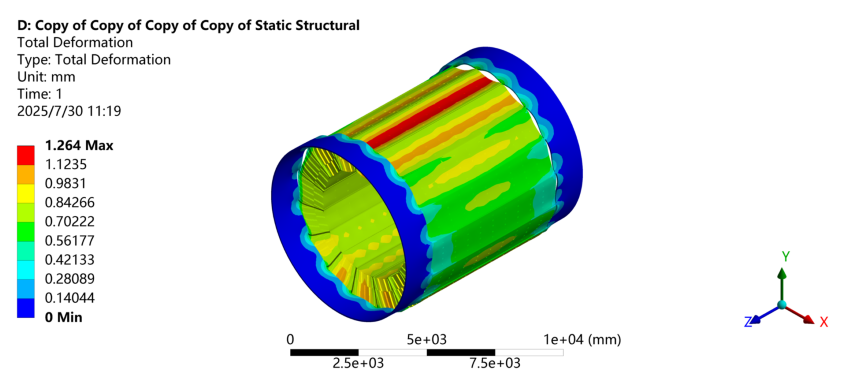
\includegraphics[width=\linewidth]{1.7.1.3.3-2.png}
  \caption{}
\end{subfigure}
\caption{Deformation distribution of the GS-HCAL barrel (a)~without
and (b)~with ECAL loading.}
\label{fig:deformation_barrel}
\end{figure}

During assembly the maximum deformation remains below \SI{0.66}{mm}
and the localised stress below \SI{190}{MPa}, well under the yield
strength.
Under the full ECAL load, peak stresses reach \SI{371}{MPa} at
specific connection points; these critical areas employ titanium-alloy
(TC4) components with safety factors above~2.2, while the bulk of the
structure is stainless steel.
Layer-to-layer deformation differences remain below \SI{0.2}{mm}
(within the \SI{2.4}{mm} gasket range), intra-layer deformations are
below \SI{0.5}{mm} inducing only \SI{20}{MPa} stress in the GS cells,
and the scintillator boxes withstand \SI{0.5}{mm} bending with a
safety factor above three.
Taken together, these results support the detector-scale mechanical
viability of the baseline concept; they are type-B evidence on the
engineering side, complementing the simulation-based detector
performance of Section~\ref{sec:simperf}.

%% --------------------------------------------------------------------
\subsection{Calibration strategy as part of the baseline architecture}
\label{subsec:calibration}
%% --------------------------------------------------------------------

Calibration is integral to the baseline concept rather than an
auxiliary activity: with 5.22~million channels and tile-to-tile light
yield variations, no operating point of the detector is reachable
without a well-defined calibration architecture.
The baseline therefore incorporates two complementary calibration
layers, physics-process calibration and hardware calibration.

\paragraph{Physics-process calibration.}
Global calibration exploits MIP signals from
$e^{+}e^{-}\to Z\to\mu^{+}\mu^{-}$ events.
At design luminosity the process rate is \SI{584}{Hz}, corresponding
to approximately 47~events per hour within a $\Delta\phi\times
\Delta\!\cos\theta=0.018\times0.018$ acceptance window matched to
one central-barrel HCAL cell (Figure~\ref{fig:kinematic_mumu}).
Bi-weekly \SI{16}{h/day} calibration runs accumulate
$4.71\times10^{8}$ di-muon events, yielding ${\sim}1\%$ statistical
precision per cell.
In addition, $e^{+}e^{-}\to Z\to q\bar{q}$ (Figure~\ref{fig:kinematic_zjj})
provides resonant dijets for combined ECAL+HCAL response
calibration through the reconstructed $m_{jj}$, and hadronic $\tau$
decays in $Z\to\tau^{+}\tau^{-}$ provide complementary $E/p$
monitoring over time.

\begin{figure}[htbp]
\centering
\begin{subfigure}{0.32\textwidth}
  \centering
  \includegraphics[width=\linewidth]{Fig8_mumu_cosTheta.pdf}
  \caption{}
\end{subfigure}\hfill
\begin{subfigure}{0.32\textwidth}
  \centering
  \includegraphics[width=\linewidth]{Fig8_mumu_phi.pdf}
  \caption{}
\end{subfigure}\hfill
\begin{subfigure}{0.32\textwidth}
  \centering
  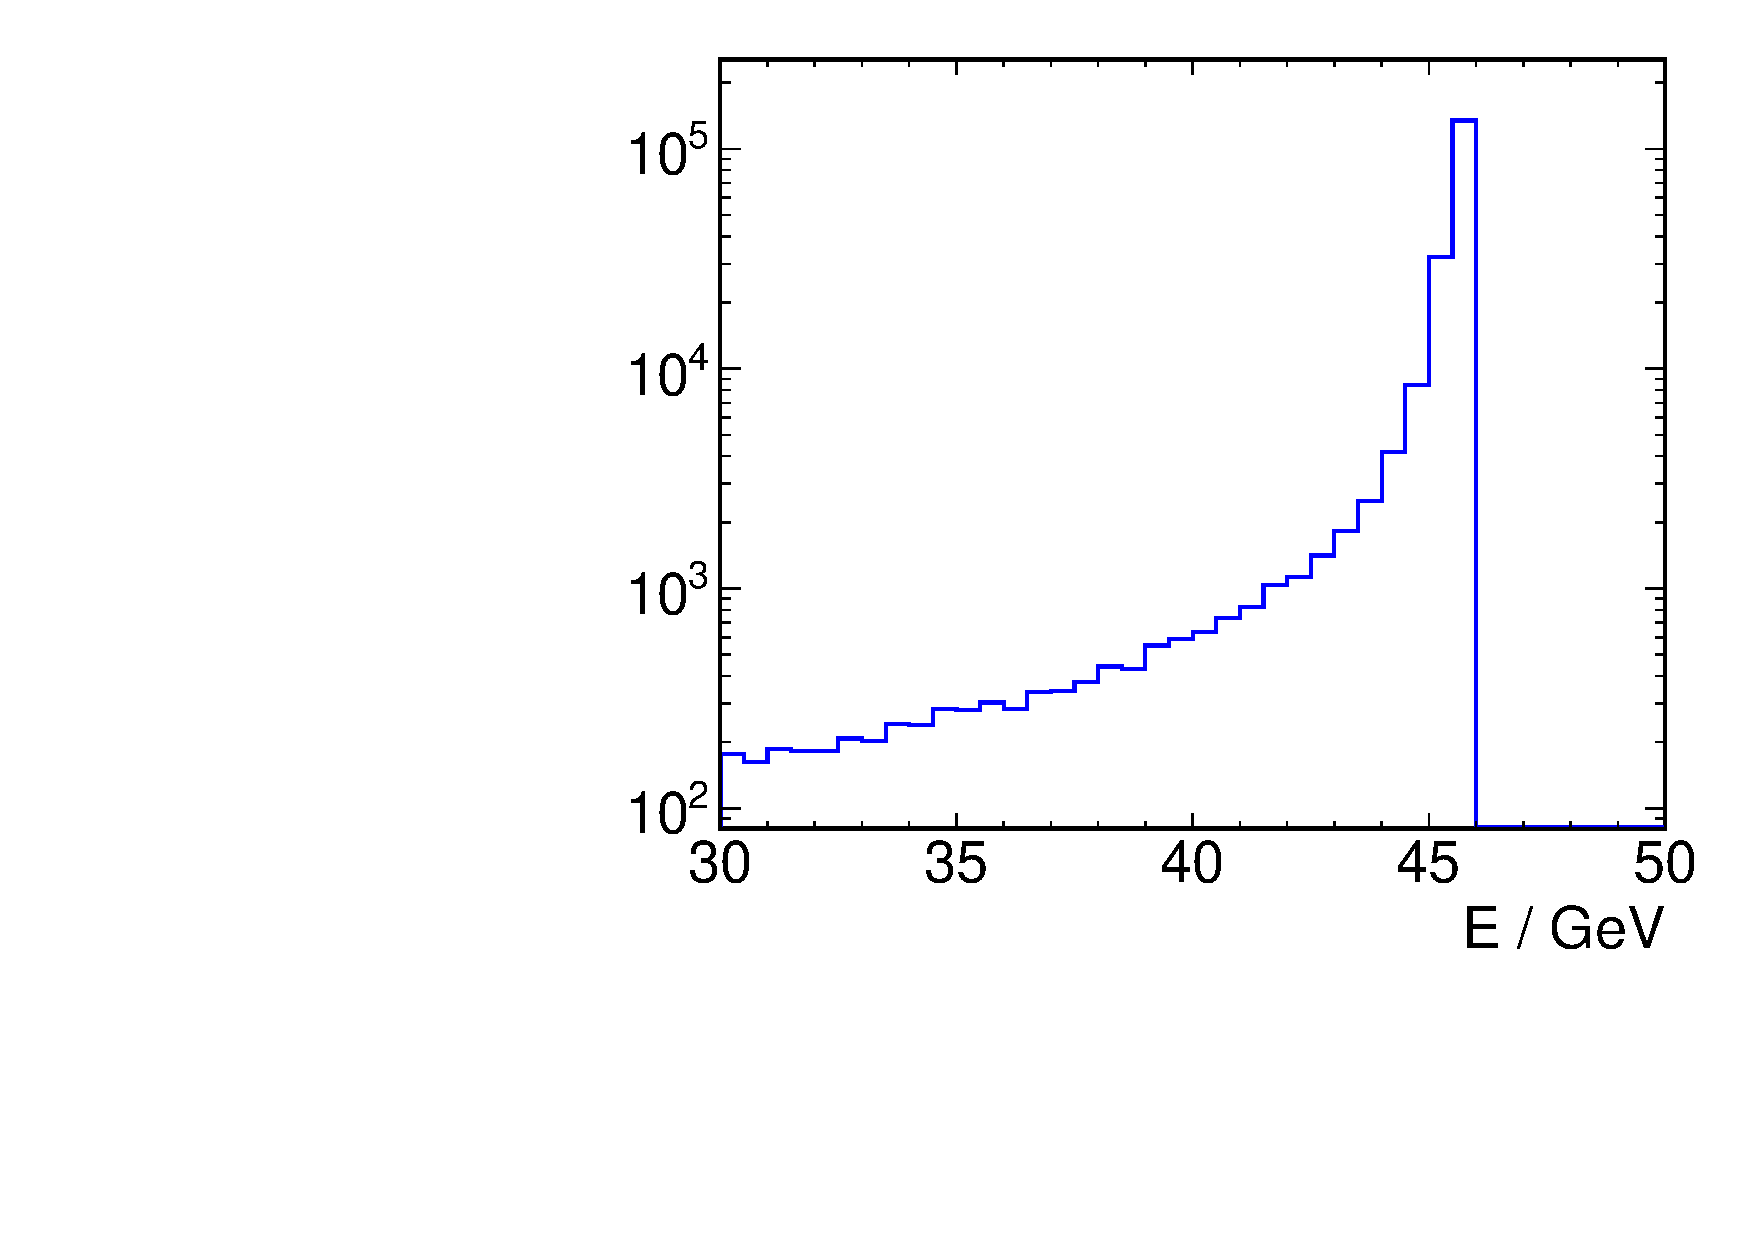
\includegraphics[width=\linewidth]{Fig8_mumu_E.pdf}
  \caption{}
\end{subfigure}
\caption{Generator-level distributions of (a)~$\cos\theta$, (b)~$\phi$,
and (c)~energy of muons in $e^{+}e^{-}\to\mu^{+}\mu^{-}$ at
$\sqrt{s}=\SI{91.2}{GeV}$.}
\label{fig:kinematic_mumu}
\end{figure}

\begin{figure}[htbp]
\centering
\includegraphics[width=0.50\textwidth]{Mjj_eeuu_91.pdf}
\caption{Distribution of dijet invariant mass from $Z\to q\bar{q}$ at
$\sqrt{s}=\SI{91.2}{GeV}$.}
\label{fig:kinematic_zjj}
\end{figure}

\paragraph{Hardware calibration.}
The hardware calibration comprises MIP inter-calibration using cosmic
rays or muon beams, and an online LED-based monitoring system with
optical-fibre distribution to multiple cells
(Figure~\ref{fig:Calibration-2n}).
The LED system continuously tracks pedestals, gain, and response
linearity at the single-cell level.

\begin{figure}[htbp]
\centering
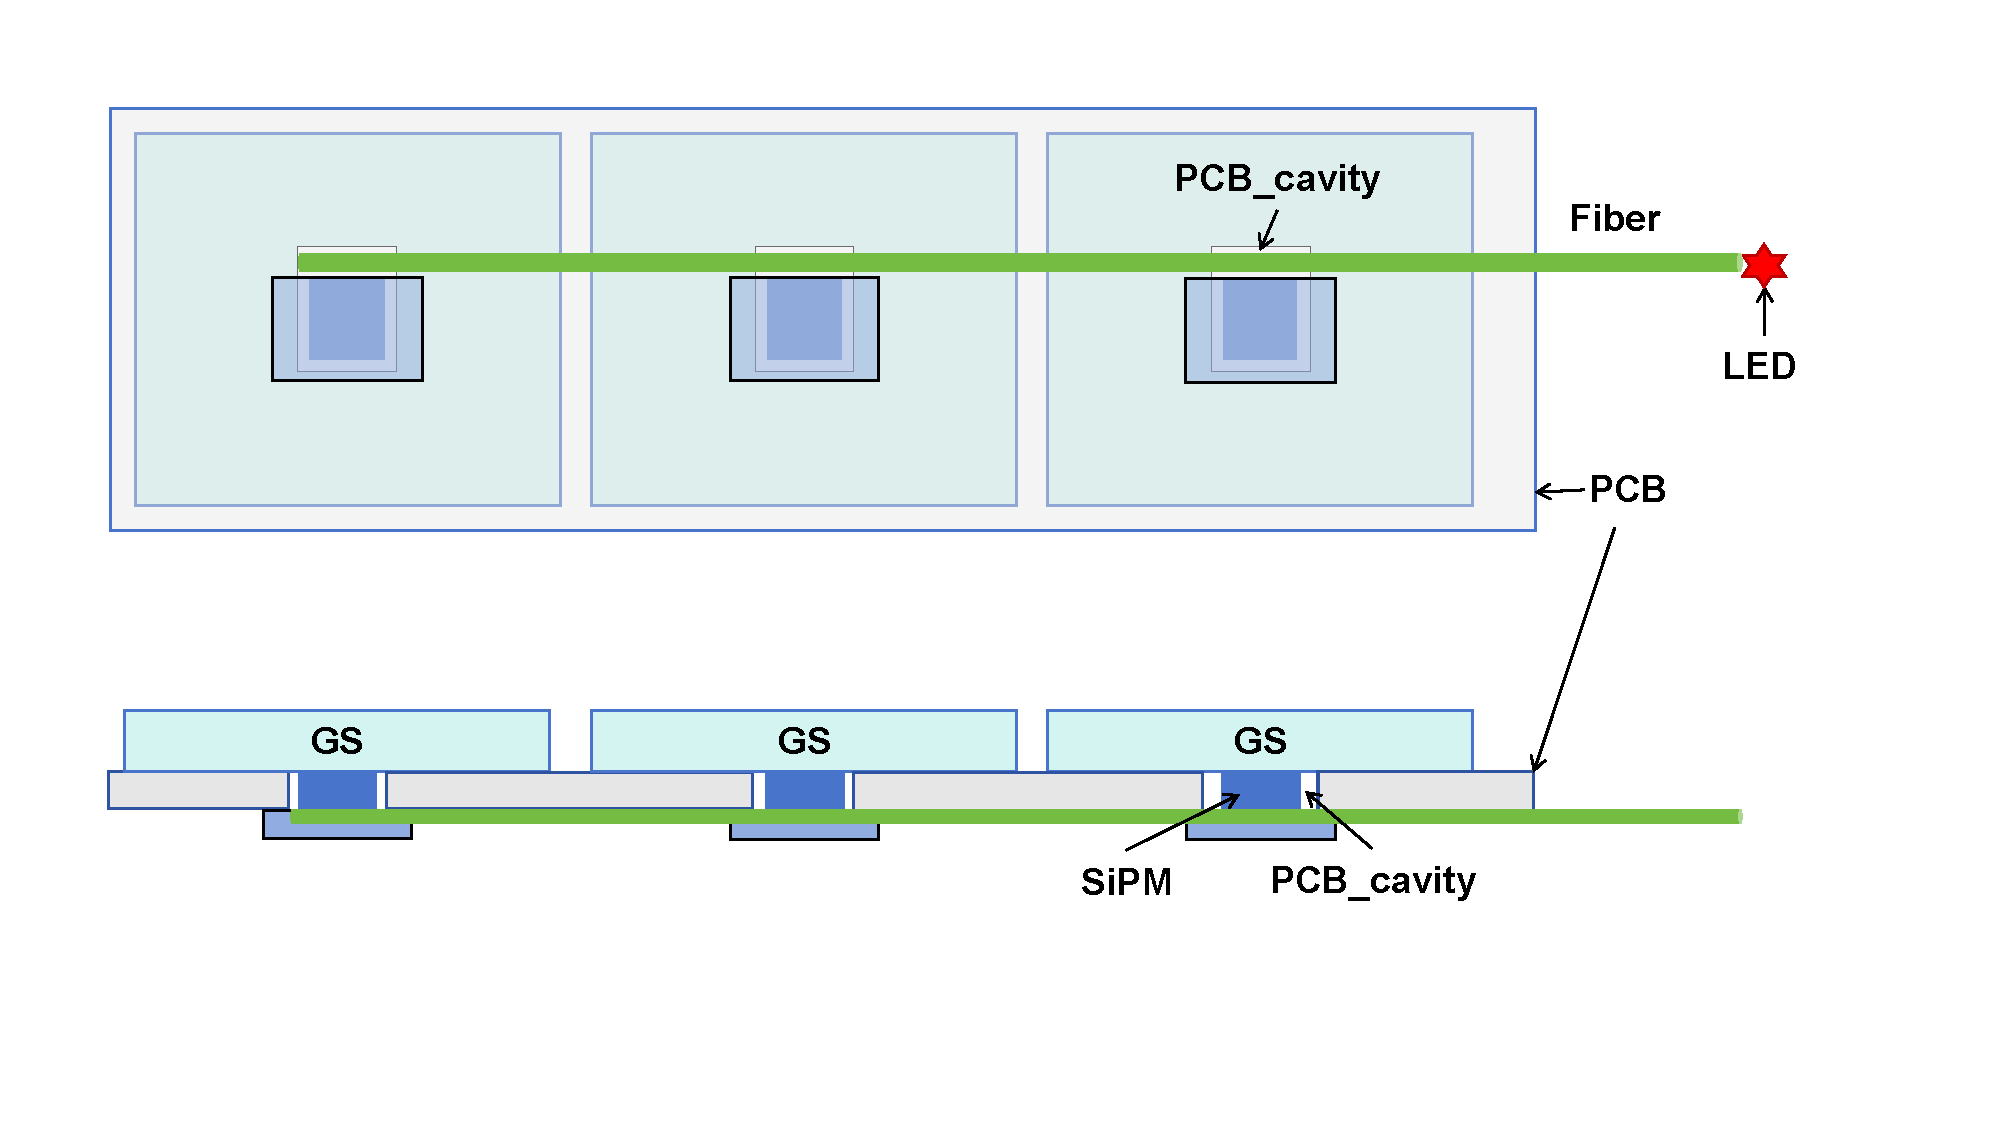
\includegraphics[width=0.68\textwidth]{Calibration-2n.pdf}
\caption{Schematic of the GS-HCAL LED calibration system showing
optical-fibre connections between adjacent cells: top~view~(a) and
side~view~(b).}
\label{fig:Calibration-2n}
\end{figure}

The two layers are complementary: the physics-process layer provides
absolute energy-scale closure in situ, while the hardware layer
provides the fast monitoring loop between physics calibrations.
The baseline design cannot be realised without both, and this is why
they are presented as components of the detector concept rather than
as post-hoc add-ons.

%% --------------------------------------------------------------------
\subsection{Prototype validation strategy}
\label{subsec:prototype}
%% --------------------------------------------------------------------

A GS-HCAL prototype is under construction to provide the validation
path of the baseline detector concept.
The prototype is a steel-scintillator sandwich of
$52.0\times52.0\times130.6$~cm$^{3}$ (${\approx}0.6$~m$^{3}$),
containing 8112~GS cells in 48~layers (${\approx}6\,\lambdaI$).
Each layer is a $13\times13$ array of \cellsize cells, each coupled
to a \sipmsize SiPM, with \SI{9.8}{mm} S304 stainless-steel absorber
plates.

Geant4 simulations with \SI{80}{GeV} $\pi^{-}$ beams show that this
$13\times13\times48$ configuration reaches 95\% energy containment
(Figure~\ref{fig:prototype-sim-energy}), and projects a prototype
single-hadron resolution of ${\sim}45\%/\sqrt{E}\oplus8\%$,
degraded relative to the full detector because of the limited
transverse extent but sufficient to validate the key baseline
technologies and reconstruction algorithms
(Figure~\ref{fig:prototype-sim-resolution}).

\begin{figure}[htbp]
\centering
\includegraphics[width=0.50\linewidth]{Edep_module_80GeV.pdf}
\caption{Simulated deposited energy in prototypes of different lateral
sizes for \SI{80}{GeV} $\pi^{-}$; the $13\times13\times48$
configuration achieves ${\approx}95\%$ containment.}
\label{fig:prototype-sim-energy}
\end{figure}

\begin{figure}[htbp]
\centering
\begin{subfigure}{0.40\textwidth}
  \centering
  \includegraphics[width=\linewidth]{prototype_simulation-13}
  \caption{}
\end{subfigure}\hfill
\begin{subfigure}{0.40\textwidth}
  \centering
  \includegraphics[width=\linewidth]{prototype_simulation-linear.jpg}
  \caption{}
\end{subfigure}
\caption{Simulated (a)~energy resolution and (b)~energy linearity of
the GS-HCAL prototype.}
\label{fig:prototype-sim-resolution}
\end{figure}

The validation proceeds in two stages:
a $3\times3\times7$ mini-prototype tests integration of the GS cell,
SiPM, front-end, and calibration at reduced scale;
the full 8112-channel prototype then exercises the complete baseline
active unit and provides the measured detector response against which
the Geant4 optical model, the Birks constant, the intrinsic $e/h$
extraction, and the constant-term interpretation can be closed.
Together with the measured containment and projected prototype
resolution, this establishes a clear closure path from the
current evidence to a fully validated baseline.

%% ====================================================================
\section{Discussion}
\label{sec:discussion}
%% ====================================================================

The foregoing sections have established the design logic, material
characterisation, simulation performance, and engineering feasibility
of the GS-HCAL baseline.
It is now useful to assess coherently what has been established, what
remains uncertain, and what the immediate validation priorities are.

%% --------------------------------------------------------------------
\subsection{What has been established}
\label{subsec:established}
%% --------------------------------------------------------------------

The baseline architecture is defined as a barrel+endcap,
$6\,\lambdaI$ deep, 48~layers of \cellsize GFO cells read out by
\sipmsize SiPMs, with approximately 5.22~million channels.
The active medium has been identified as GFO glass, with measured
intrinsic light yield $>\SI{1000}{\phMeV}$, attenuation length
${\sim}\SI{6}{cm}$, and radiation tolerance retaining more than 70\%
of the initial light yield at \SI{100}{Gy}.
Cell-level readout feasibility is demonstrated by single-cell
measurements with $^{137}$Cs, cosmic-ray muons
(${63.6\pm0.5}$~\peMIP), and \SI{5}{GeV} electrons at KEK
(${157.6\pm2.9}$~\peMIP), and by the interim pre-amplifier
performance.
SiPM compatibility with the baseline cell is demonstrated by the DCR
versus threshold behaviour at the \SI{0.1}{MIP} working point.
Full digitisation-based system simulation predicts a single-hadron
energy resolution of $29.8\%/\sqrt{E}\oplus6.5\%$ and an $H\to gg$
BMR of 3.88\%, consistent with the CEPC target of 3--4\%.
Mechanical finite-element analysis demonstrates feasibility at
detector scale.
A two-layer calibration architecture has been defined as an integral
part of the baseline.

%% --------------------------------------------------------------------
\subsection{What remains uncertain}
\label{subsec:uncertain}
%% --------------------------------------------------------------------

The following items have \emph{not} yet been experimentally closed
and collectively define the open boundary of the baseline:

\begin{itemize}
\item \textbf{Full-prototype beam validation} is not yet complete; the
  8112-channel prototype is under construction and its beam-test
  closure is the principal missing experimental step.
\item \textbf{Geant4 optical parameters} for GFO require tuning: the
  simulated single-cell light yield (${\sim}42$~\peMIP) is below the
  measured cosmic-ray value (${\sim}64$~\peMIP).
\item \textbf{Birks' constant} used in the digitisation model is
  preliminary; a dedicated heavy-ion measurement is planned.
\item \textbf{Intrinsic $e/h$} has not yet been extracted through
  shower-component decomposition; only the empirical
  $C_{\mathrm{hadron}}/C_{e}$ is currently available.
\item \textbf{Constant term} of ${\approx}5$--6\% is linked to
  longitudinal leakage; its expected reduction with full-detector
  environment and software compensation is demonstrated only in
  simulation.
\item \textbf{Tile production yield and uniformity} still require
  optimisation: only about 60\% of produced tiles currently meet the
  \SI{1000}{\phMeV} target.
\end{itemize}

%% --------------------------------------------------------------------
\subsection{Why these uncertainties do not invalidate the baseline
choice}
\label{subsec:rationale-uncertainty}
%% --------------------------------------------------------------------

A baseline choice in a detector concept does not require that every
uncertainty be closed simultaneously and in advance.
What it requires is that the combined evidence identifies a single
integrated technology direction that is already supported at the
material, cell, system, and engineering levels, and that the
remaining uncertainties are well localised, fully characterised,
and attached to an explicit closure path.
The present GS-HCAL results satisfy this criterion: the baseline
architecture, the active medium, the readout, the simulation
framework, and the calibration and mechanical strategies all stand on
measured or simulation-based evidence, while the open items of
Section~\ref{subsec:uncertain} are individually attached to the
prototype programme of Section~\ref{subsec:prototype} and to the
immediate priorities below.

%% --------------------------------------------------------------------
\subsection{Immediate priorities}
\label{subsec:priorities}
%% --------------------------------------------------------------------

The immediate priorities are:
\begin{itemize}
\item prototype beam tests, to provide the first measured closure of
  the detector-level response;
\item Geant4 optical-model tuning against measured GFO data, to
  close the simulation--measurement discrepancy on the single-cell
  light yield;
\item intrinsic $e/h$ extraction and implementation of software
  compensation, to bring the constant term towards the final target;
\item development of the low-power ASIC and its system-level
  integration.
\end{itemize}

%% ====================================================================
\section{Conclusion}
\label{sec:conclusion}
%% ====================================================================

The Glass-Scintillator HCAL is adopted as the baseline HCAL of the
CEPC reference detector, and the present study establishes the design
logic and technical basis of that choice.

The baseline evidence combines measured GFO material performance,
single-cell readout demonstrated with three independent probes, SiPM
operation at a working threshold compatible with the measured dark
count rate, full-detector Geant4 digitisation predicting a
single-hadron resolution of $29.8\%/\sqrt{E}\oplus6.5\%$ and an
$H\to gg$ BMR of 3.88\%, detector-scale mechanical feasibility, and a
calibration architecture integrated into the detector concept from
the outset.
These measured, simulated, and engineering lines of evidence are
coherent and together support the baseline.

Full prototype beam tests remain essential for the final experimental
validation of the baseline detector concept; they are the next step
in closing the items listed in Section~\ref{subsec:uncertain}, and
they define the validation path from the present technical basis to a
fully validated baseline HCAL.

%% ====================================================================
\section*{Acknowledgements}
%% ====================================================================

The authors thank all members of the CEPC Study Group for their
contributions to the physics and detector design studies.
We are grateful to the CALICE Collaboration for extensive test-beam
data and collaborative R\&D efforts, and to the staff of the KEK
test-beam facility and the APEP proton-irradiation facility for
experimental support.
This work is supported in part by
the National Key Research and Development Program of China
(Grant No.~2020YFA0406200),
the Chinese Academy of Sciences (Grant No.~XDB34000000),
the National Natural Science Foundation of China (NSFC,
Grant Nos.~12075265 and~12105295),
and the CEPC detector R\&D programme.

%% ====================================================================
%% References
%% ====================================================================
%% The bibliography style is set by each wrapper via \bibliostyle
%% before %% ====================================================================
%% GS-HCAL paper — shared body text
%% Baseline detector-technology paper for the CEPC reference detector
%% ====================================================================

%% ====================================================================
\section{Introduction}
\label{sec:intro}
%% ====================================================================

The Circular Electron-Positron Collider
(CEPC)~\cite{CEPCStudyGroup:2018ghi} will operate as a Higgs factory at
$\sqrt{s}=240$~GeV and as a high-luminosity $Z$-pole machine at
$\sqrt{s}=91.2$~GeV.
Within the Particle-Flow Algorithm
(PFA)~\cite{Thomson:2009rp,Brient:2004yq,Ruan:2013rkk} paradigm, the
Hadronic Calorimeter (HCAL) is responsible for the precise spatial
reconstruction and energy measurement of neutral hadrons, which carry
approximately 10\% of the jet energy and leave no tracks in the central
tracker.
The target boson mass resolution (BMR) of
3--4\%~\cite{CEPCStudyGroup:2018ghi} for $W$/$Z$/Higgs dijet final
states directly depends on the HCAL performance.
These requirements are satisfied only when the HCAL simultaneously
provides fine three-dimensional granularity, sufficient depth, and
adequate energy resolution.

The baseline choice is driven not by a single metric, but by the
combined requirements of neutral-hadron measurement, high granularity
for particle flow, compactness, active-material density, scalable cell
production, SiPM-compatible readout, and detector-scale integration.
The Glass-Scintillator HCAL
(GS-HCAL)~\cite{Tang:2022yrb,Hu:2023dbm,Hu:2024nvo} is adopted as the
baseline HCAL of the CEPC reference detector because it is the only
mature integrated technology that satisfies all of these requirements
simultaneously, while being supported by measured material performance,
validated single-cell readout, full-detector digitisation simulation,
and an established mechanical and calibration concept.
Alternative HCAL technologies exist, but they are outside the scope of
this paper.

The remainder of this paper reports:
the physics- and technology-driven design requirements and the
rationale for the baseline choice (Section~\ref{sec:rationale});
the detector-scale architecture and system design
(Section~\ref{sec:design});
the active-unit implementation, comprising the GFO glass, the SiPM
readout, the front-end electronics, and the supporting optical
simulation (Section~\ref{sec:activeunit});
the experimental characterisation of the baseline active unit
(Section~\ref{sec:expchar});
the simulation framework and projected detector performance
(Section~\ref{sec:simperf});
the mechanical feasibility, calibration strategy, and prototype
validation path (Section~\ref{sec:feasibility});
a discussion of established results and remaining uncertainties
(Section~\ref{sec:discussion});
and a concluding summary (Section~\ref{sec:conclusion}).

\begin{figure}[htbp]
\centering
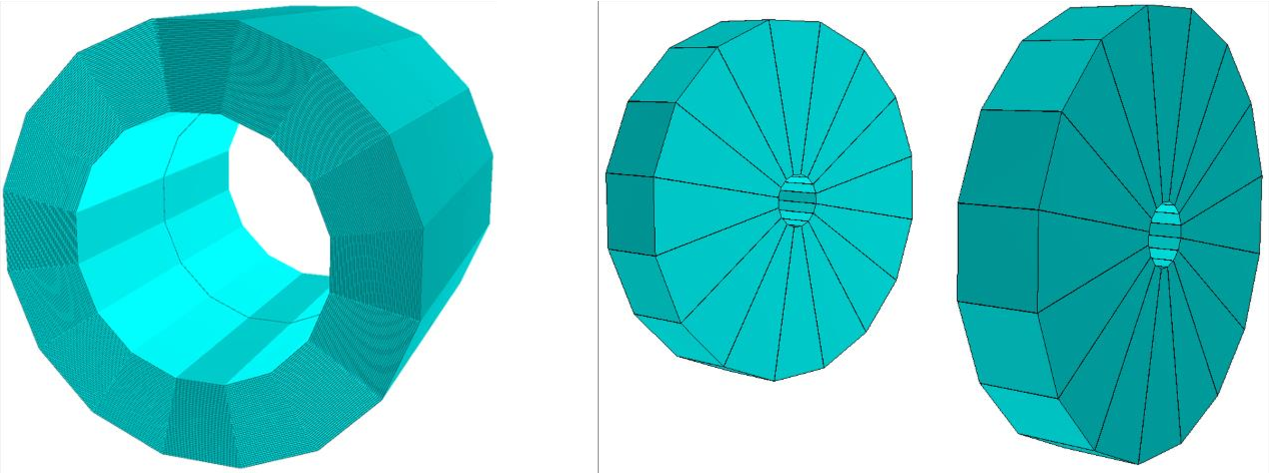
\includegraphics[width=0.9\textwidth]{Geometry.pdf}
\caption{Geometric configuration of the GS-HCAL system.
Left: barrel with 16~trapezoidal sectors forming a cylindrical structure
(inner diameter \SI{4280}{mm}, outer diameter \SI{6910}{mm}).
Right: endcap disks with matching sector segmentation.}
\label{fig:GS-geometry}
\end{figure}

%% ====================================================================
\section{Design requirements and baseline rationale}
\label{sec:rationale}
%% ====================================================================

The adoption of the GS-HCAL as the baseline HCAL of the CEPC
reference detector rests on the convergence of three independent lines
of argument: the physics requirements imposed by the CEPC programme
and the PFA paradigm; the technology requirements that any candidate
HCAL must simultaneously satisfy; and the specific combination of
measured and simulated properties that makes GS-HCAL the most mature
integrated technology satisfying all of them together.

%% --------------------------------------------------------------------
\subsection{Physics-driven requirements}
\label{subsec:physics-req}
%% --------------------------------------------------------------------

In the PFA paradigm the HCAL must independently measure neutral
hadrons---primarily neutrons and $K_{L}^{0}$ mesons---that leave no
tracks in the central tracker and carry approximately 10\% of the jet
energy.
These particles are the dominant source of resolution degradation in
PFA jet reconstruction, because their energy must be taken directly
from the calorimeter rather than from the tracker.
The CEPC target BMR of 3--4\% for $W/Z$/Higgs dijet final states
therefore translates into stringent HCAL requirements:
\begin{itemize}
\item Fine three-dimensional granularity is required to separate
  neutral-hadron clusters from nearby charged-particle energy deposits
  and to enable longitudinal shower analysis.
\item Sufficient depth, typically $\gtrsim6\,\lambdaI$ in the
  HCAL~itself, is required to contain hadronic showers and minimise
  longitudinal leakage.
\item The energy response must be close to linear and well-calibrated
  across the relevant range (${\sim}0.5$--\SI{60}{GeV}) so that PFA
  reconstruction of jet substructure remains robust.
\item Good single-hadron resolution also benefits searches for
  long-lived particles that may decay within the HCAL volume.
\end{itemize}

%% --------------------------------------------------------------------
\subsection{Technology-driven requirements}
\label{subsec:tech-req}
%% --------------------------------------------------------------------

Any HCAL technology candidate for the CEPC reference detector must
simultaneously satisfy the following integrated requirements:

\begin{itemize}
\item \textbf{Active-medium density:} higher density reduces the
  detector envelope for a fixed number of nuclear interaction lengths,
  which is critical in the limited radial budget of the reference
  detector.
\item \textbf{Cell granularity at the $40\times40$~mm$^{2}$ scale:}
  required for PFA shower separation; must be reproducibly
  manufacturable at that scale.
\item \textbf{SiPM-compatible light output:} the active medium must
  produce enough scintillation light that a compact SiPM readout can
  operate at a \SI{0.1}{MIP} threshold while suppressing dark-count
  noise.
\item \textbf{Scalability to approximately 5.22~million channels:} the
  production, assembly, and quality-control procedures must be
  compatible with the resulting system-level complexity.
\item \textbf{Radiation tolerance:} optical performance must be
  retained under the accumulated doses expected during Higgs and
  $Z$-pole operation.
\item \textbf{Thermal and electronics integration:} the front-end
  electronics, cooling, and mechanical support must be accommodated
  within the available layer thickness.
\item \textbf{Modular assembly feasibility:} the detector must be
  buildable, installable, and serviceable at realistic engineering
  tolerances.
\end{itemize}

These requirements must be satisfied \emph{together}---a technology
that excels in only a subset of them is not a viable baseline.

%% --------------------------------------------------------------------
\subsection{Why GS-HCAL is adopted as the baseline}
\label{subsec:why-baseline}
%% --------------------------------------------------------------------

The GS-HCAL is adopted as the baseline because the combined evidence
from materials R\&D, single-cell measurements, full-detector
digitisation simulation, and engineering analysis shows that it is the
most mature technology that satisfies the requirements of
Sections~\ref{subsec:physics-req} and~\ref{subsec:tech-req}
simultaneously.
The supporting evidence is of three distinct types, which are kept
separate throughout this paper:
(A)~experimentally measured properties of GFO cells and SiPM readout;
(B)~full-detector Geant4 digitisation simulation of the baseline
geometry; and (C)~analyses whose final closure depends on ongoing
prototype beam tests.

Specifically, the baseline choice is supported by the following five
points.

\begin{enumerate}
\item \textbf{Active-medium density (A).}
  GFO glass provides a density of \SI{6.0}{g/cm^{3}}, substantially
  higher than plastic scintillator (${\sim}\SI{1.03}{g/cm^{3}}$),
  while remaining manufacturable at the $40\times40\times10$~mm$^{3}$
  cell scale and delivering a measured intrinsic light yield
  $>\SI{1000}{\phMeV}$ (Sections~\ref{subsec:gfo}
  and~\ref{subsec:lightyield}).
\item \textbf{Cell geometry and PFA compatibility (A+B).}
  The \cellsize cell geometry, combined with \sipmsize SiPM readout,
  is compatible with highly granular PFA calorimetry; measured
  single-cell light outputs of 60--100~\peMIP
  (Section~\ref{subsec:cellmeas}) establish that practical SiPM
  operation is achievable at the required threshold.
\item \textbf{Radiation tolerance (A).}
  The GFO light yield retains more than 70\% of its initial value at
  \SI{100}{Gy} (Section~\ref{subsec:radiation}), which covers the
  accumulated dose expected over the CEPC operational scenarios.
\item \textbf{Projected detector performance (B).}
  Full digitisation-based Geant4 simulation of the baseline geometry
  predicts a single-hadron energy resolution of
  $\sigma_{E}/E = 29.8\%/\sqrt{E}\oplus6.5\%$ and an $H\to gg$ BMR of
  3.88\%, consistent with the CEPC target of 3--4\%
  (Sections~\ref{subsec:hadronres} and~\ref{subsec:physperf}).
\item \textbf{Detector-scale feasibility (A+B).}
  Finite-element analysis of the modular-box architecture demonstrates
  mechanical feasibility under the full load including the ECAL, and
  the water-cooling and calibration concepts are compatible with the
  channel count and dissipation
  (Sections~\ref{subsec:architecture}--\ref{subsec:channels}
  and~\ref{subsec:mechanics}).
\end{enumerate}

Categories~A and~B together establish the technical basis of the
baseline.
Final experimental closure, category~C, requires prototype beam tests
and is the subject of Section~\ref{subsec:prototype}.

%% --------------------------------------------------------------------
\subsection{Boundaries and remaining work}
\label{subsec:boundaries}
%% --------------------------------------------------------------------

The baseline rationale is transparent about what has \emph{not} yet
been experimentally closed.
Before proceeding to the detailed design and characterisation, the
principal boundaries of the current evidence are summarised here:

\begin{itemize}
\item Full prototype beam validation has not yet been performed; the
  8112-channel prototype is under construction
  (Section~\ref{subsec:prototype}).
\item The Geant4 optical model of GFO requires further tuning: the
  simulated single-cell light yield (${\sim}42$~\peMIP) is lower
  than the cosmic-ray measurement (${\sim}64$~\peMIP)
  (Section~\ref{subsec:optsim}).
\item The Birks constant used in the digitisation model is
  preliminary; a dedicated heavy-ion measurement is planned
  (Section~\ref{subsec:simsetup}).
\item The intrinsic $e/h$ compensation ratio has not yet been
  extracted from shower-component decomposition
  (Section~\ref{subsec:eresponse}).
\item The constant term (${\approx}5$--6\%) is currently dominated by
  longitudinal leakage in the $6\,\lambdaI$ design
  (Section~\ref{subsec:constterm}).
\item Tile production yield and light-yield uniformity still require
  optimisation: at present only about 60\% of produced tiles exceed
  the \SI{1000}{\phMeV} target (Section~\ref{subsec:qc}).
\end{itemize}

These items are discussed systematically in
Section~\ref{sec:discussion}.
They define the validation path of the baseline, but they do not
invalidate the baseline choice itself: a baseline identifies the most
mature and best-supported integrated technology direction, not a
concept whose every uncertainty is already experimentally closed.

%% ====================================================================
\section{Baseline detector concept and system design}
\label{sec:design}
%% ====================================================================

The baseline concept is realised at detector scale through a
barrel-plus-endcap architecture with 48~longitudinal layers of
\cellsize GFO cells.
Each design choice is driven by one or more of the requirements
established in Section~\ref{sec:rationale}, and the motivation is
given before the corresponding parameters.

%% --------------------------------------------------------------------
\subsection{Overall architecture}
\label{subsec:architecture}
%% --------------------------------------------------------------------

The overall architecture is driven by three requirements:
hermetic geometric coverage for PFA, sufficient depth for hadronic
containment, and a granularity compatible with shower separation in
the CEPC jet environment.
These requirements are met by a barrel with two endcaps, each
segmented into 16~trapezoidal sectors of 48~longitudinal layers and a
total depth of $6\,\lambdaI$ in steel and GS
(Figure~\ref{fig:GS-geometry}).
The barrel has inner and outer radii of \SI{2140}{mm} and
\SI{3455}{mm} and a length of \SI{6460}{mm} along the beam axis; the
endcaps match this segmentation with inner and outer radii of
\SI{450}{mm} and \SI{3455}{mm}.
The complete detector contains approximately 5.22~million identical
\cellsize GFO cells, each read out by a \sipmsize SiPM; the
corresponding sampling fraction is approximately 31\%.

%% --------------------------------------------------------------------
\subsection{Single-layer design as the fundamental baseline unit}
\label{subsec:onelayer}
%% --------------------------------------------------------------------

The single-layer design is the fundamental unit of the baseline
detector concept.
It is chosen so that the active GS layer, the SiPM plus PCB readout,
the ASIC cooling, and the steel absorber all fit within a compact
layer thickness while preserving the sampling fraction and mechanical
tolerances required by the PFA design.
Each layer has a total thickness of \SI{27.2}{mm}, corresponding to
approximately $0.125\,\lambdaI$, and contains from top to bottom:
a \SI{2}{mm} upper cover plate;
the \SI{10}{mm} GS active layer of $40\times40$~mm$^{2}$ cells;
a \SI{3.2}{mm} PCB layer carrying the front-end ASICs;
a \SI{2}{mm} bottom cover; and
a \SI{9.8}{mm} steel absorber in which cooling pipes of \SI{3}{mm}
outer radius are embedded.
One SiPM is positioned at the centre of each GS cell on a PCB shared
by multiple cells.
The nuclear-interaction-length contributions of the steel absorber,
the GS active layer, and the PCB are in the ratio $1:0.53:0.03$,
giving a sampling fraction of approximately 31\%.

\begin{figure}[htbp]
\centering
\begin{subfigure}{0.50\linewidth}
  \centering
  \includegraphics[width=\linewidth]{GS-HCAL-cell.pdf}
  \caption{}
  \label{fig:gshcal-cell-a}
\end{subfigure}%
\begin{subfigure}{0.35\linewidth}
  \centering
  \includegraphics[width=\linewidth]{GSHCALOneCell1.pdf}
  \caption{}
  \label{fig:gshcal-cell-b}
\end{subfigure}
\caption{(a)~Single-layer structure of the GS-HCAL\@.
(b)~One GS cell of \cellsize.}
\label{fig:gshcal-cell}
\end{figure}

%% --------------------------------------------------------------------
\subsection{Barrel implementation}
\label{subsec:barrel}
%% --------------------------------------------------------------------

The barrel is divided into 16~trapezoidal sectors
(Figure~\ref{fig:BarrelContourDimension}), each having a front width
of \SI{851}{mm}, a back width of \SI{1375}{mm}, and a radial thickness
of \SI{1315}{mm} ($6\,\lambdaI$).
The longitudinal segmentation into 48~layers follows the PFA
optimisation performed with the Plastic-Scintillator HCAL
prototype~\cite{CALICE:2010fpb}.
The total barrel weight is \SI{955}{t}
(Table~\ref{tab:BarrelWeight}).

Each layer consists of a continuous steel absorber plate over the full
barrel length, onto which modular detection boxes are mounted.
Each box contains a complete detection unit---GS cells, SiPMs, PCB,
ASICs, cables, and cover plates---with three standard box widths
(\SI{320}{mm}, \SI{280}{mm}, \SI{240}{mm}) combined to follow the
trapezoidal geometry while preserving the uniform \cellsize~cell
granularity (Figure~\ref{fig:BarrelModuleStructure}).
The 16~radial sector boundaries introduce projective cracks, but these
are effectively compensated by the upstream BGO ECAL
(${\approx}1.2\,\lambdaI$), which initiates most hadronic showers
before the HCAL and produces lateral spread bridging the sector
boundaries.

\begin{figure}[htbp]
\centering
\begin{subfigure}{0.42\linewidth}
  \centering
  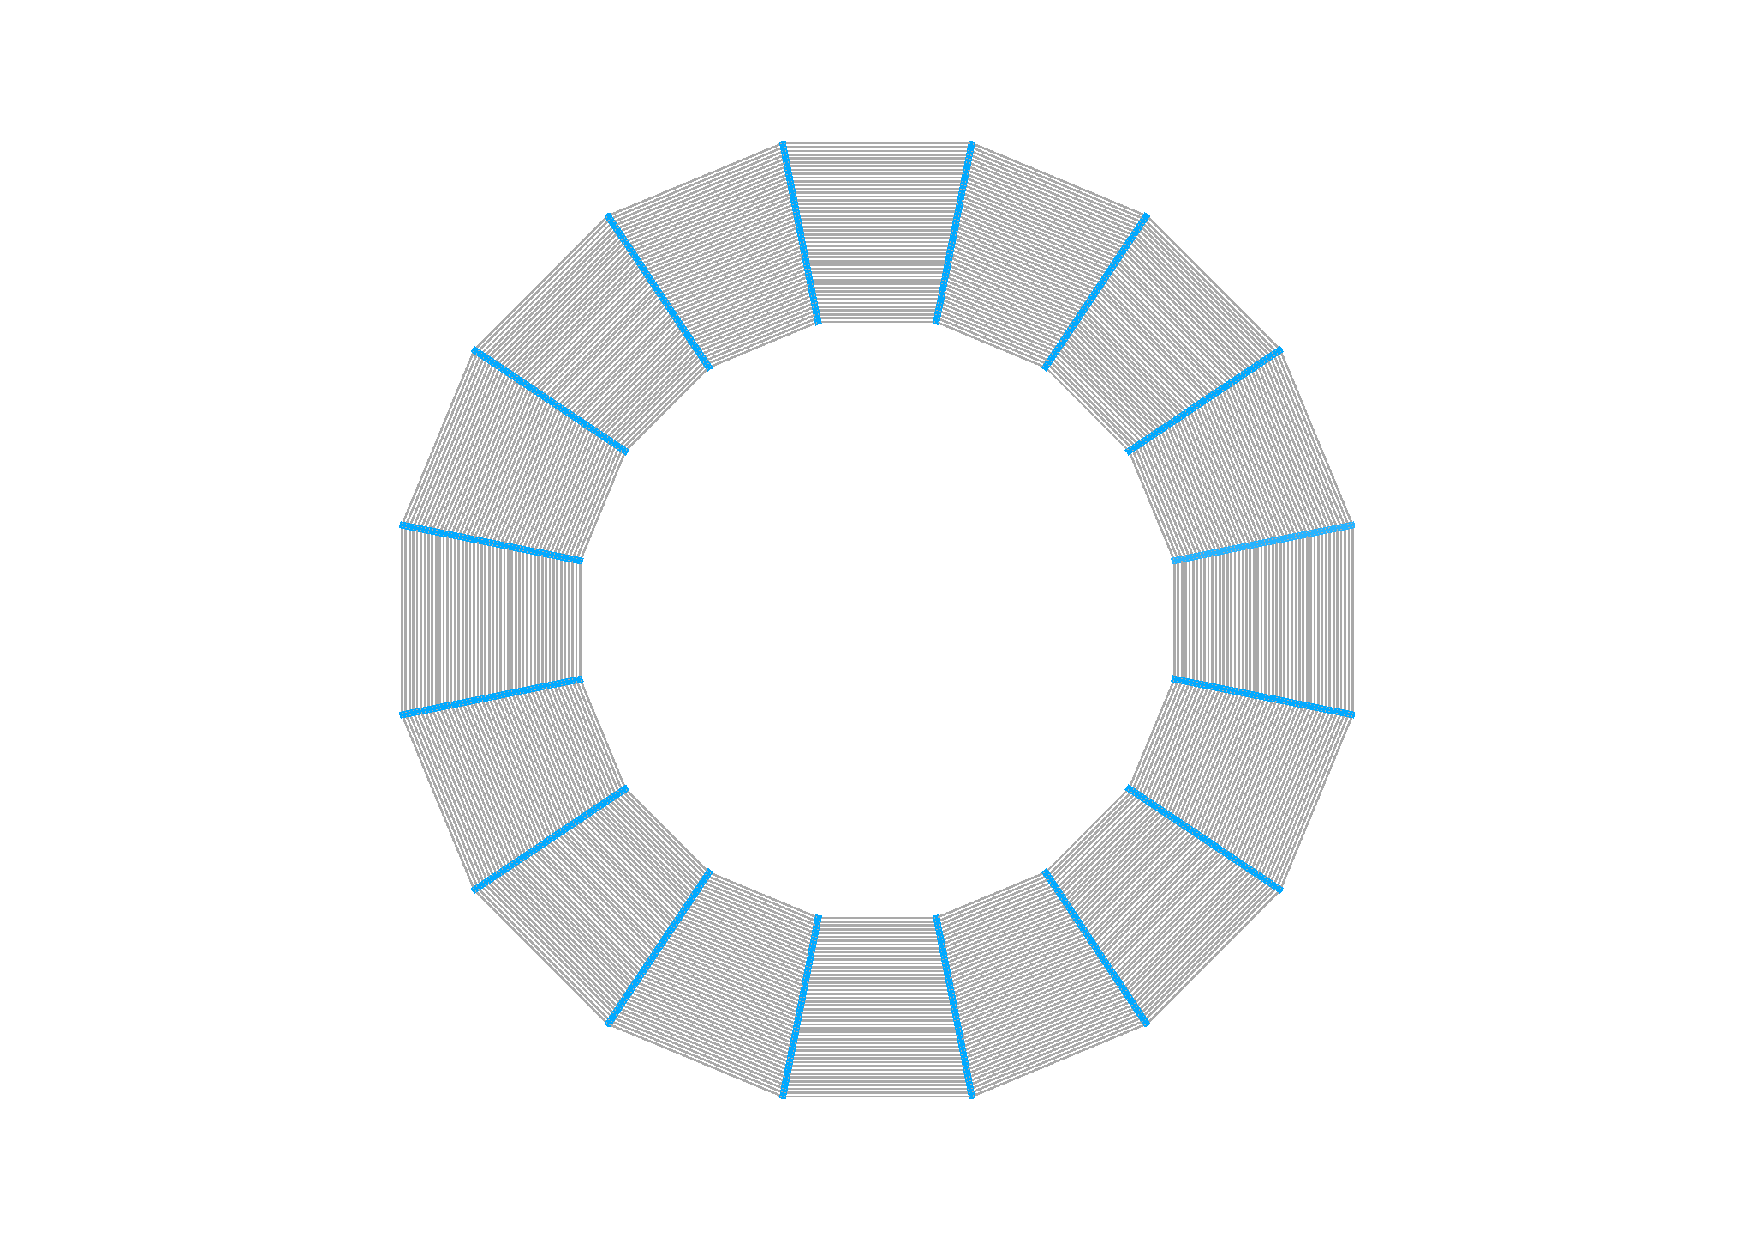
\includegraphics[width=\linewidth,trim=160pt 50pt 160pt 50pt,clip]{BarrelView1.pdf}
  \caption{}
\end{subfigure}\hfill
\begin{subfigure}{0.45\linewidth}
  \centering
  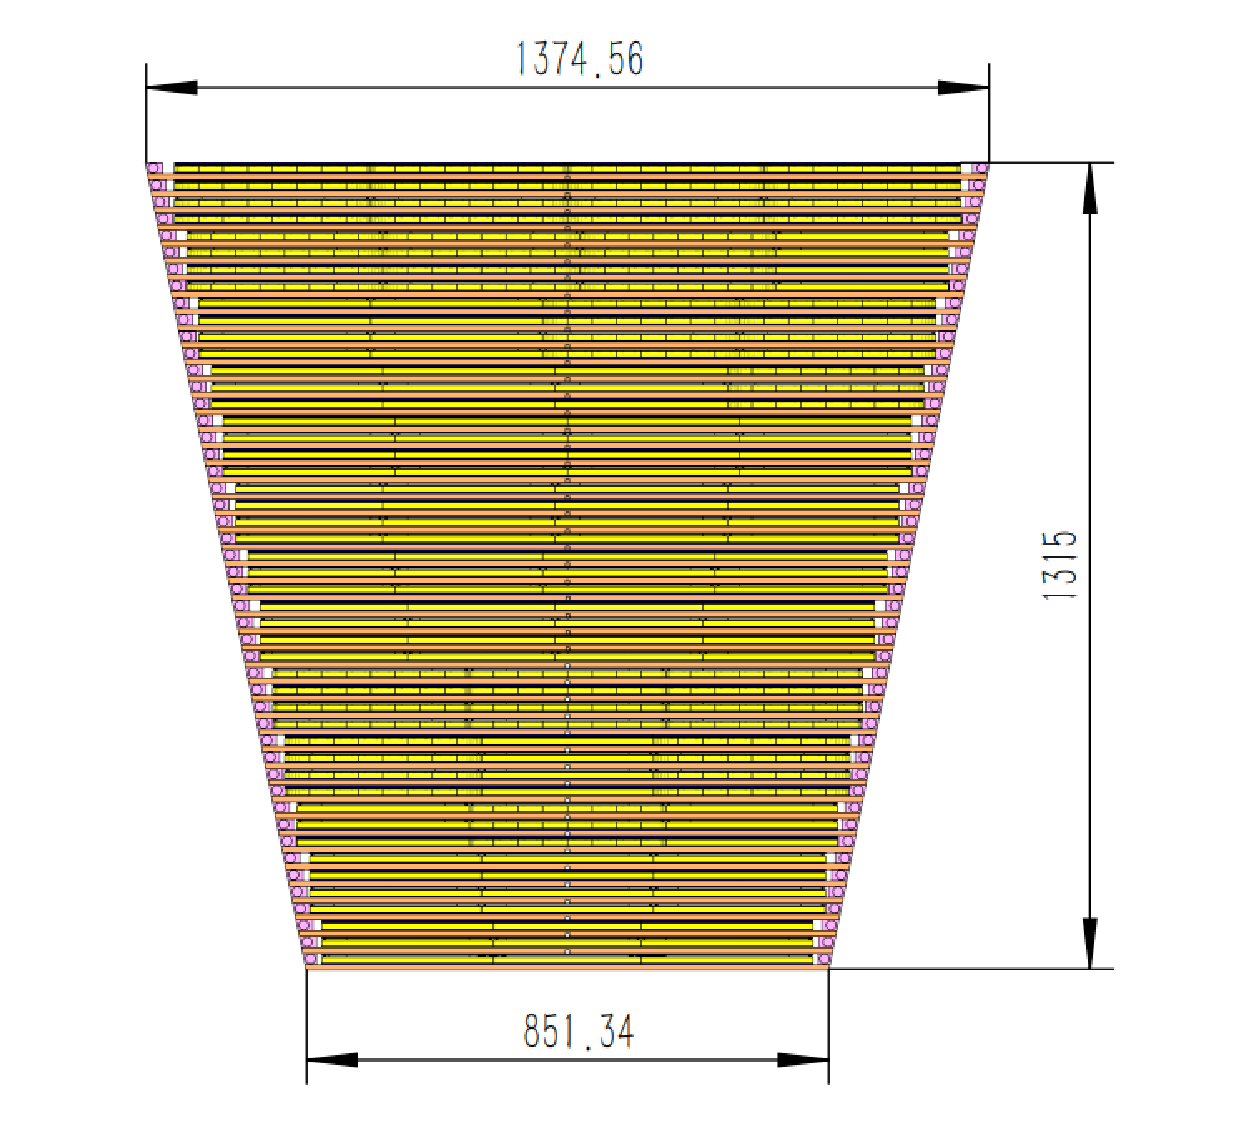
\includegraphics[width=\linewidth]{HCALBarrelOneSector.pdf}
  \caption{}
\end{subfigure}
\caption{Dimensions of the GS-HCAL barrel.
(a)~Cross-sectional view showing 16~trapezoidal sectors
(inner diameter \SI{4280}{mm}, outer diameter \SI{6910}{mm}).
(b)~Side view of a single trapezoidal sector.}
\label{fig:BarrelContourDimension}
\end{figure}

\begin{figure}[htbp]
\centering
\includegraphics[width=0.9\linewidth]{Fig.1.81-Boxes_dimension-and_more-structure_details.pdf}
\caption{GS-HCAL barrel sector structure.
(a)~Full sector composed of 48~layers.
(b)~Dimensions of an individual box.
(c)~Internal structure of a box with cover plates, GS cells, PCB
with ASICs, cables, and cooling-water pipes.}
\label{fig:BarrelModuleStructure}
\end{figure}

\begin{table}[htbp]
\centering
\caption{Weight breakdown of the barrel GS-HCAL\@.}
\label{tab:BarrelWeight}
\begin{tabular}{l S[table-format=5.0] S[table-format=3.1]}
\toprule
\textbf{Component} & {\textbf{Weight/sector (kg)}} & {\textbf{Weight/barrel (t)}} \\
\midrule
Cover plate        & 10287 & 164.6 \\
PCB plate          &   390 &   6.2 \\
Glass scintillator & 19277 & 308.4 \\
Absorber layer     & 27515 & 440.2 \\
Support structure  &  1883 &  30.1 \\
Auxiliaries        &   350 &   5.6 \\
\midrule
Total              & 59702 & 955.2 \\
\bottomrule
\end{tabular}
\end{table}

%% --------------------------------------------------------------------
\subsection{Endcap implementation}
\label{subsec:endcap}
%% --------------------------------------------------------------------

The two endcaps complete the geometric coverage along the beam
direction (Figure~\ref{fig:EndcapsOverall}).
Each endcap mirrors the barrel segmentation with 16~disk-shaped
sectors, inner and outer radii of \SI{450}{mm} and \SI{3455}{mm}, and a
total thickness of \SI{1315}{mm} in 48~layers.
A single sector has a top width of \SI{1307}{mm} and a radial height of
\SI{2862}{mm}, and is divided radially into six boxes.
Each endcap weighs \SI{362}{t}.

\begin{figure}[htbp]
\centering
\begin{subfigure}{0.58\linewidth}
  \centering
  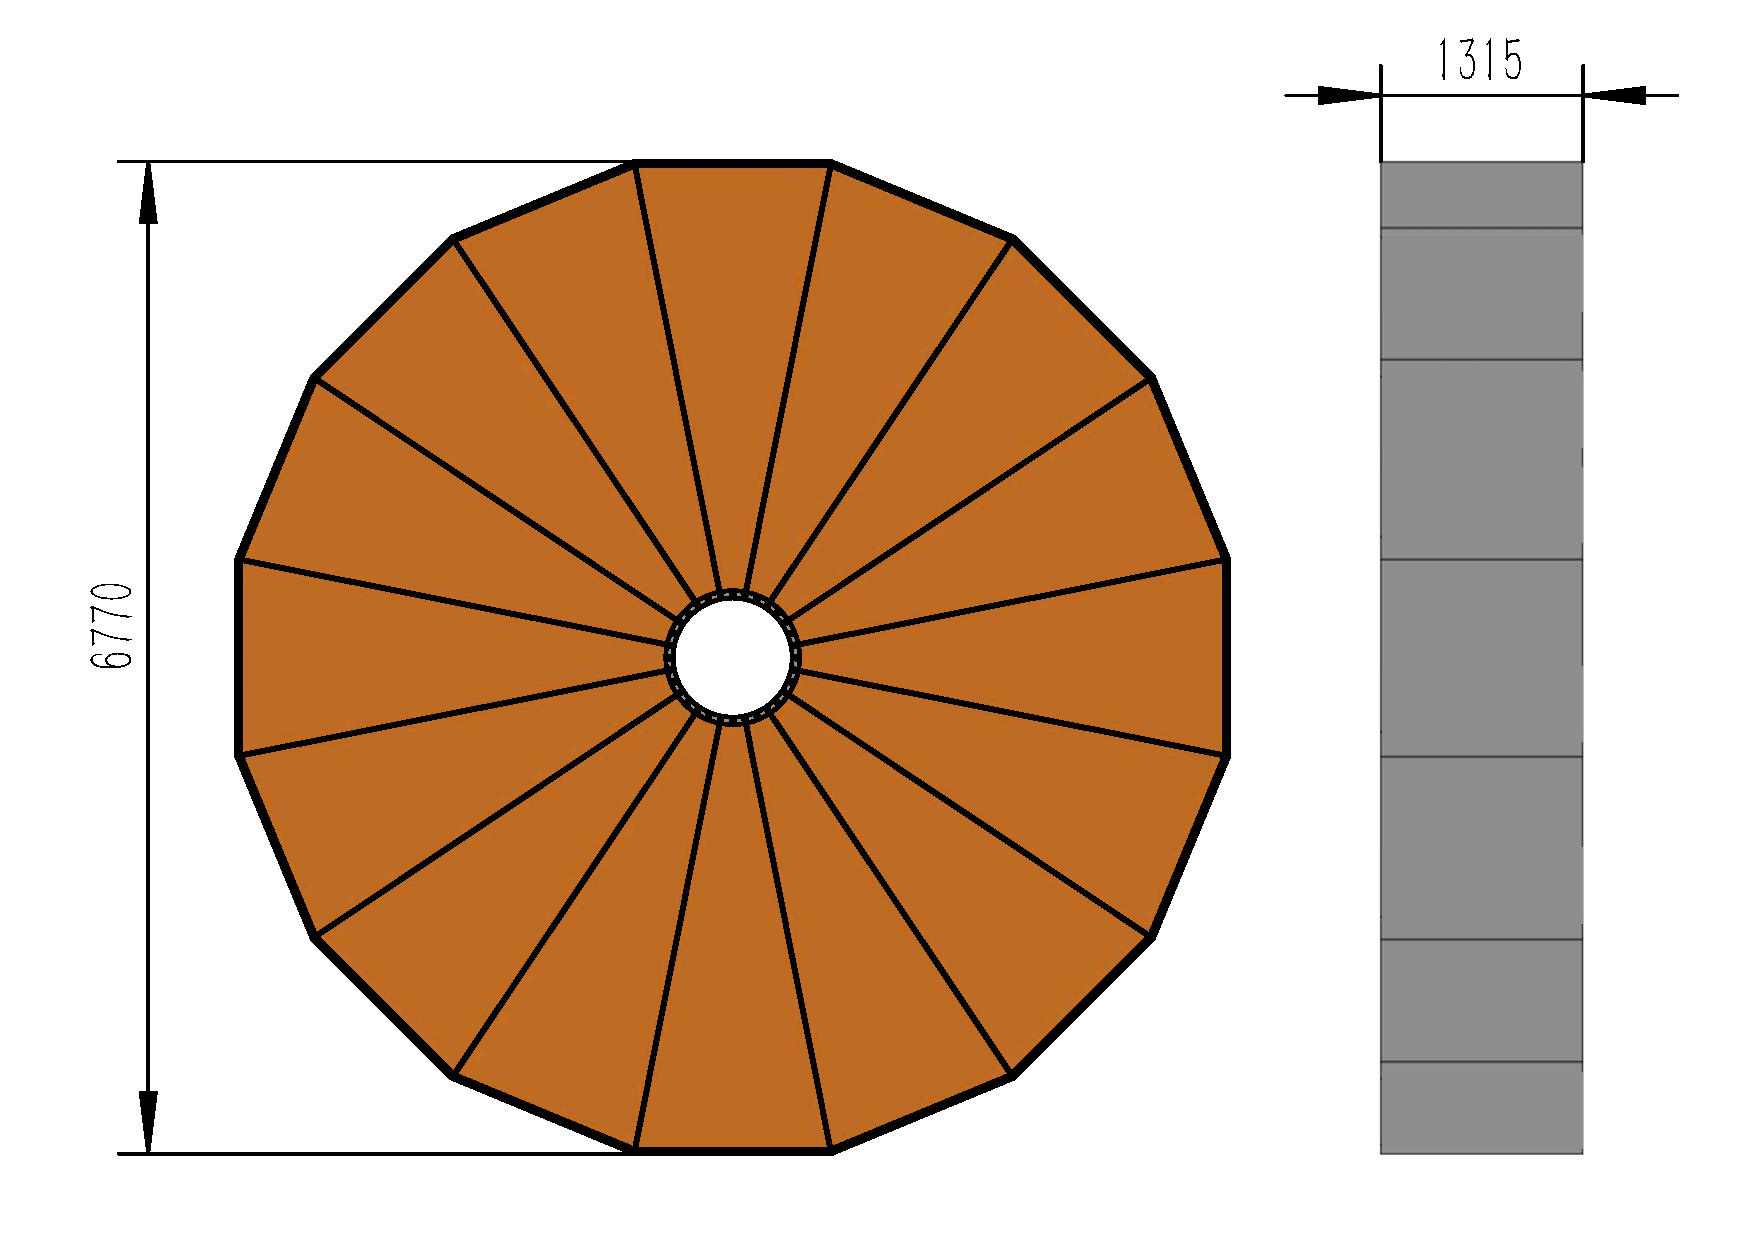
\includegraphics[width=\linewidth]{HCALEndcapOverall.pdf}
  \caption{}
\end{subfigure}\hfill
\begin{subfigure}{0.20\linewidth}
  \centering
  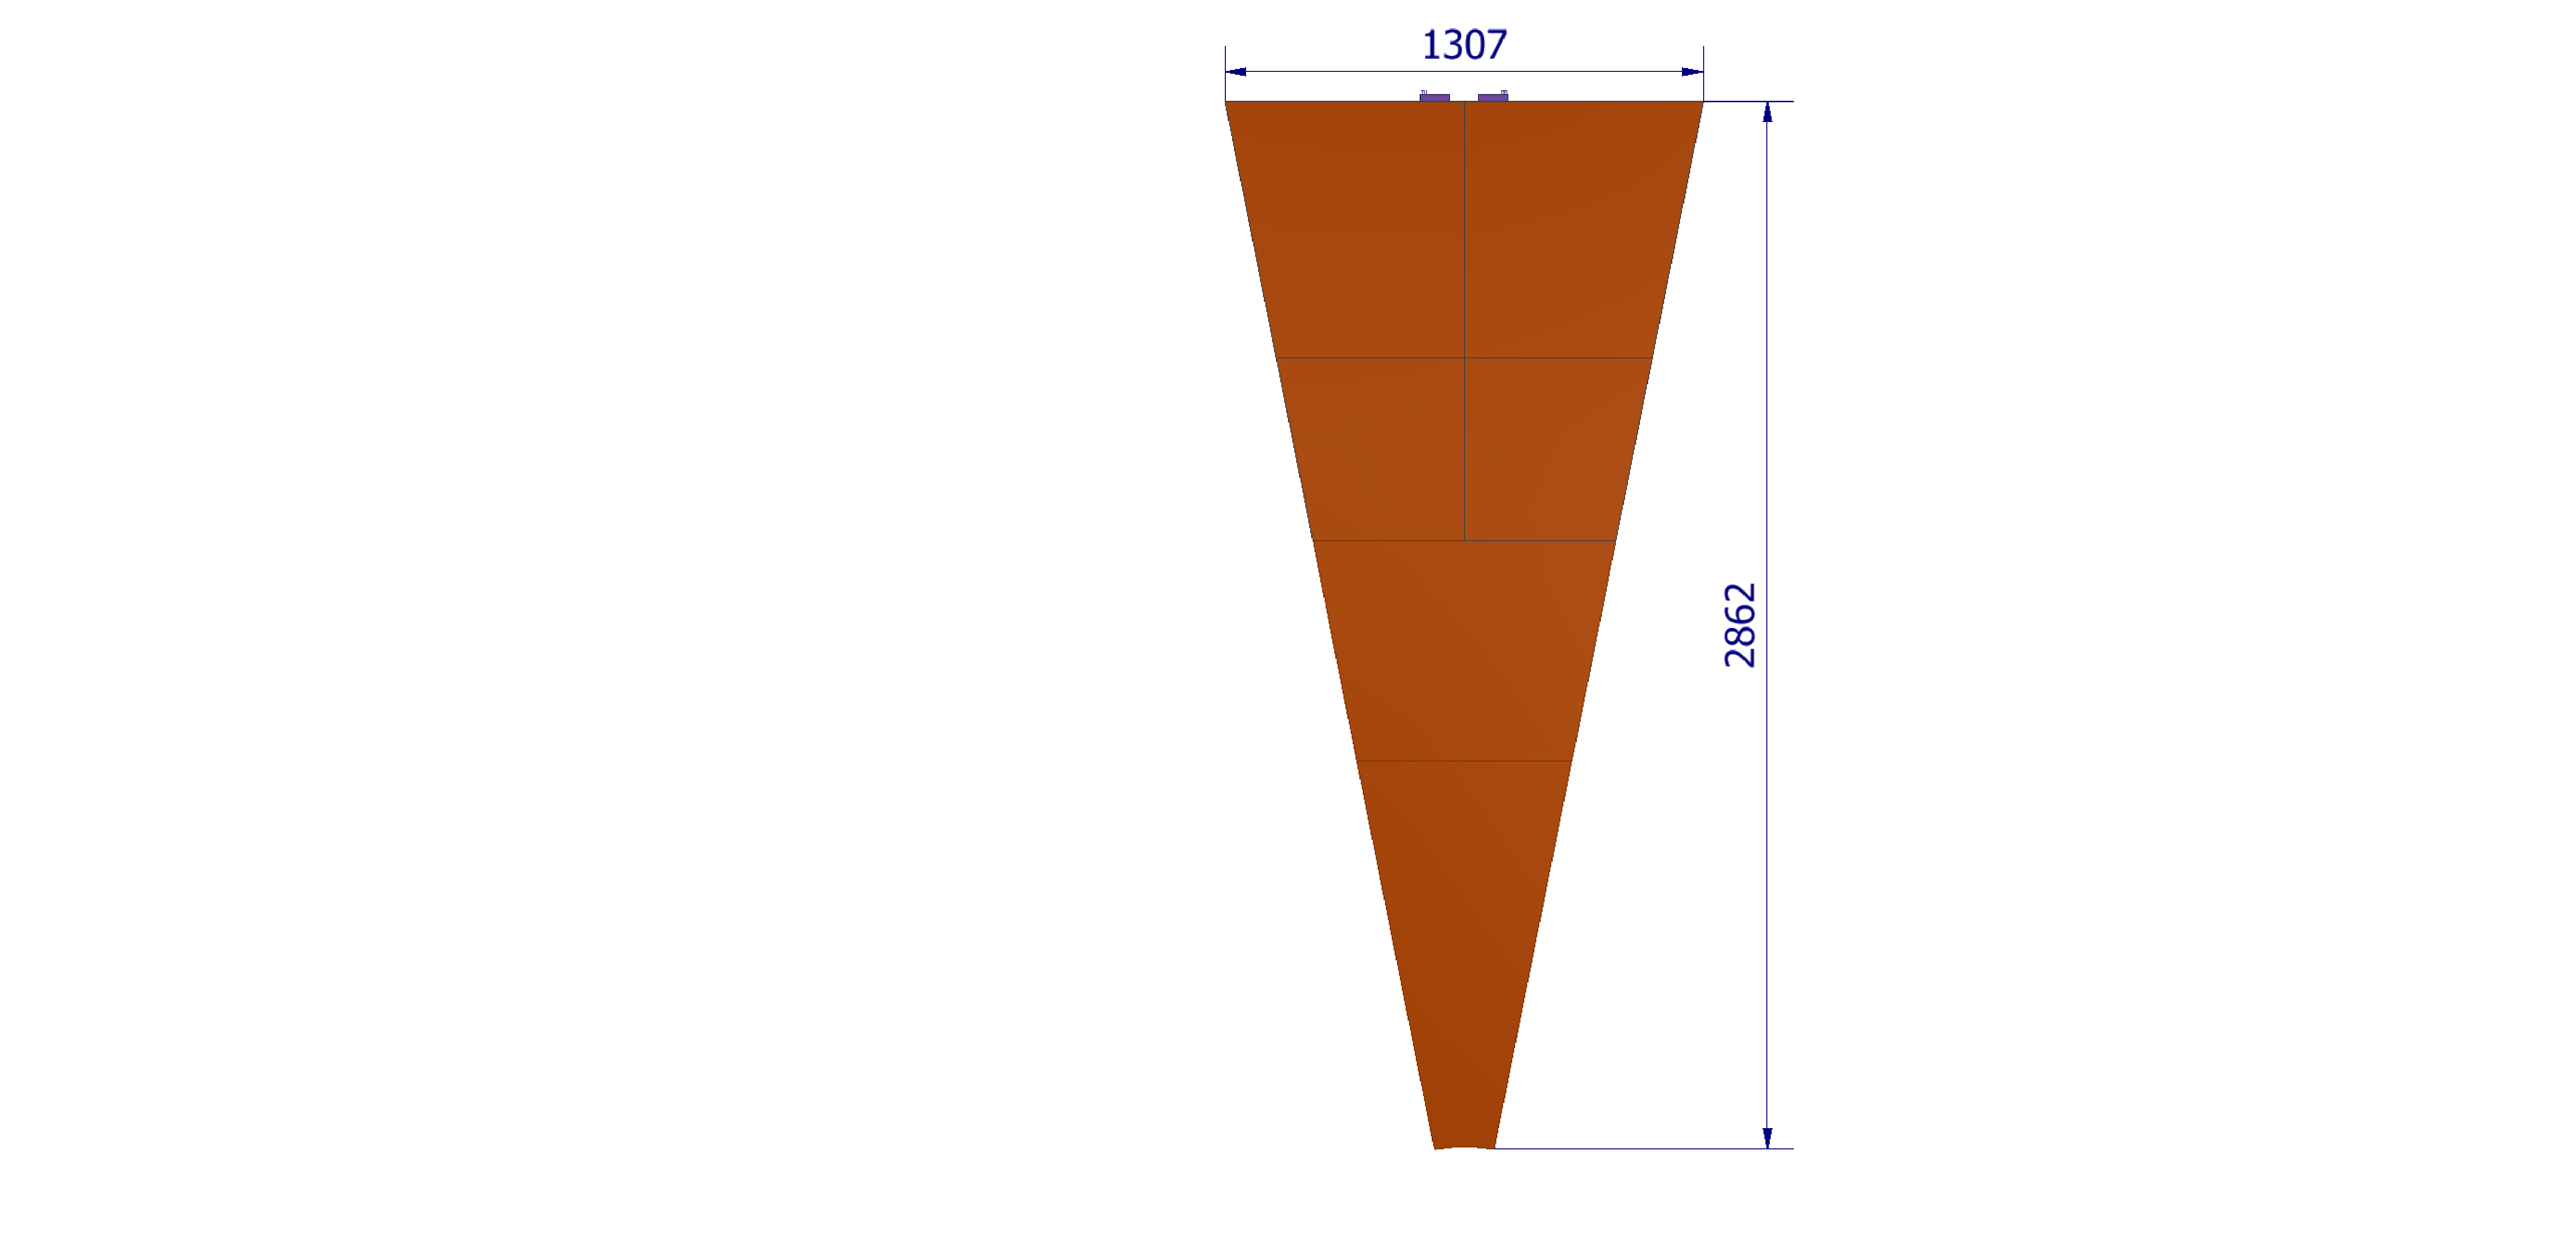
\includegraphics[width=\linewidth]{HCALEndcapOneSector.pdf}
  \caption{}
\end{subfigure}
\caption{Dimensions of the GS-HCAL endcaps.
(a)~Front and side views.
(b)~A single endcap sector.}
\label{fig:EndcapsOverall}
\end{figure}

%% --------------------------------------------------------------------
\subsection{Services: cooling, routing, and modular assembly}
\label{subsec:cooling}
%% --------------------------------------------------------------------

Service integration is an integral part of the baseline concept
because the 5.22~million channels and \SI{15}{mW/channel} ASIC power
impose non-trivial thermal and routing constraints on any practical
realisation.
A water-cooling system manages the front-end thermal load.
In the barrel, four cooling pipes are embedded in the steel absorber
of each layer, and every eight consecutive layers share common
manifolds to form six independent cooling loops per sector
(Figure~\ref{fig:BarrelCooling}).
In the endcap, 16~cooling regions per layer connect vertically across
all 48~layers to form 48~parallel circuits
(Figure~\ref{fig:M-14}).
The modular box architecture, combined with the eight-in-one cooling
topology, also provides clear routing paths for cables and gas, and
supports in-layer access during assembly and maintenance.

\begin{figure}[htbp]
\centering
\begin{subfigure}{0.55\linewidth}
  \centering
  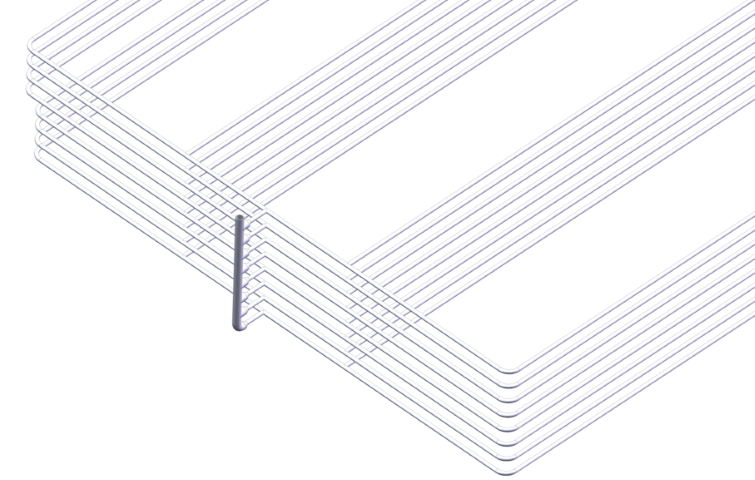
\includegraphics[width=\linewidth]{CoolingBarrelLeft.png}
  \caption{}
\end{subfigure}\hfill
\begin{subfigure}{0.35\linewidth}
  \centering
  \includegraphics[width=\linewidth]{CoolingBarrelv2.jpg}
  \caption{}
\end{subfigure}
\caption{Cooling-pipe routing for a barrel sector.
(a)~Schematic of the eight-in-one pipeline design.
(b)~Simulated coolant flow-velocity distribution.}
\label{fig:BarrelCooling}
\end{figure}

\begin{figure}[htbp]
\centering
\begin{subfigure}{0.50\linewidth}
  \centering
  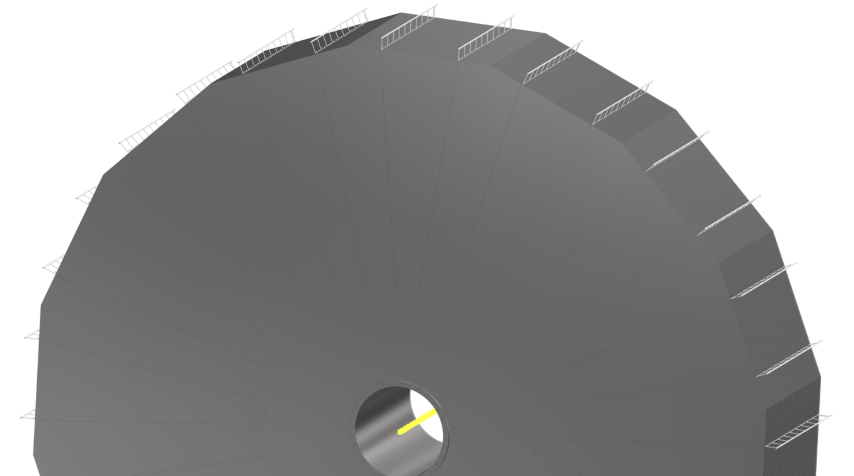
\includegraphics[width=\linewidth]{CoolingEndcapHalf.png}
  \caption{}
\end{subfigure}\hfill
\begin{subfigure}{0.42\linewidth}
  \centering
  \raisebox{0.1cm}{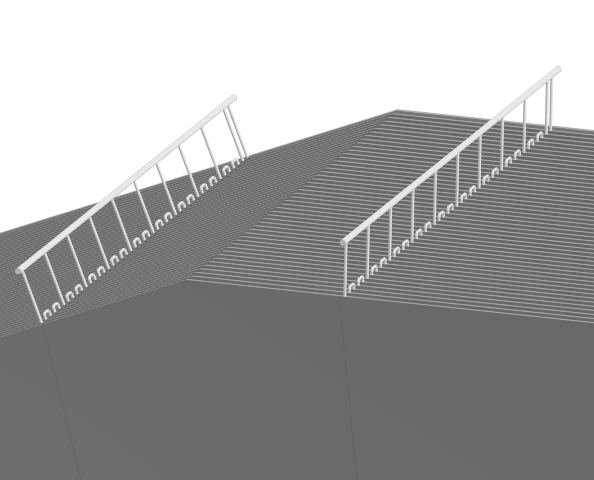
\includegraphics[width=\linewidth]{CoolingEndcapPart.png}}
  \caption{}
\end{subfigure}
\caption{Endcap cooling-pipe structure: (a)~half of the endcap;
(b)~zoomed corner view.}
\label{fig:M-14}
\end{figure}

%% --------------------------------------------------------------------
\subsection{Channel count and detector-scale implications}
\label{subsec:channels}
%% --------------------------------------------------------------------

Table~\ref{tab:GSHCALQuantities} summarises the cell, box, layer, and
sector counts.
The complete detector contains approximately 5.22~million readout
channels.
This number is itself a baseline-level design constraint:
it fixes the scale of ASIC production, calibration infrastructure
(Section~\ref{subsec:calibration}), and modular assembly
(Section~\ref{subsec:prototype}), and it is the principal driver of the
low-power per-channel requirement.
The baseline numbers are therefore chosen so that each of these
detector-scale dependencies is simultaneously feasible rather than
optimised independently.

\begin{table}[htbp]
\centering
\caption{Numbers of cells, boxes, layers, and sectors for the barrel
and the two endcaps.}
\label{tab:GSHCALQuantities}
\begin{tabular}{lcccc}
\toprule
\textbf{Part} & \textbf{Cells} & \textbf{Boxes} & \textbf{Layers} &
\textbf{Sectors} \\
\midrule
Barrel             & 3\,212\,800          & 27\,840        & $48\times16$
& 16 \\
Endcap ($\times2$) & $1\,006\,080\times2$ & $3072\times2$  &
$48\times16\times2$ & $16\times2$ \\
\bottomrule
\end{tabular}
\end{table}

%% ====================================================================
\section{Glass scintillator, photosensor, and front-end implementation}
\label{sec:activeunit}
%% ====================================================================

The baseline active unit---the GFO cell, the SiPM, the front-end
electronics, and the supporting optical simulation---constitutes the
primary technology chain of the GS-HCAL.
Each component is characterised as part of this integrated chain,
because the performance of any element is meaningful only in the
context of the others.

%% --------------------------------------------------------------------
\subsection{Choice of GFO glass as the baseline active medium}
\label{subsec:gfo}
%% --------------------------------------------------------------------

High-$Z$ glass scintillators have been investigated for calorimetry
since the 1980s~\cite{Buchner:1988fu}, but early attempts were limited
by short radiation length, low light yield, and strong self-absorption
in long-bar geometries.
The maturation of SiPM technology and PFA-oriented highly granular
calorimetry changed this picture: compact optically isolated cells of
${\sim}\SI{1}{cm}$-scale thickness eliminate the long-path
self-absorption problem, so that a moderate light yield of
${\sim}\SI{1000}{\phMeV}$ combined with a modern SiPM becomes
sufficient for practical readout~\cite{Tang:2022yrb,Hu:2023dbm,
Hu:2024nvo}.

Building on this opportunity, the Glass-Scintillator Collaboration has
systematically developed high-$Z$ glass
compositions~\cite{LAN2022113000,YU2023113846,ZHU2024} targeting the
density--light-yield trade-off with manufacturability at the
\cellsize cell scale (Figure~\ref{fig:GSGroup}).
Gadolinium fluoro-oxide (GFO) glass is adopted as the baseline active
medium because it combines high density, manufacturable tile geometry,
and adequate optical properties in a single
material~\cite{HUA202523367,Hua:2023myf,Hua:2024djh}.
Its key parameters are listed in Table~\ref{tab:GS1} alongside BGO
crystal~\cite{BGO} and DSB glass~\cite{Dormenev:2021vtn} for
reference.
GFO achieves a density of \SI{6.0}{g/cm^{3}} with a radiation length of
\SI{1.59}{cm} and a nuclear interaction length of \SI{24.2}{cm}.
The Ce$^{3+}$ luminescent centre provides strong emission near
\SI{400}{nm} with efficient energy transfer from Gd$^{3+}$
modifiers~\cite{GS-1}; the borosilicate matrix provides thermal and
optical stability; and the use of gadolinium, rather than lanthanum or
lutetium, provides a favourable combination of density, intrinsic
radioactivity, and cost.
These properties are directly matched to the \cellsize cell
requirement.

\begin{figure}[htbp]
\centering
\includegraphics[width=0.7\textwidth]{GSGroup.pdf}
\caption{Light yield versus density for GS samples developed by the
Glass-Scintillator Collaboration and by other groups.}
\label{fig:GSGroup}
\end{figure}

\begin{table}[htbp]
\centering
\caption{Key parameters of GFO glass ($5\times5\times5$~mm$^{3}$
sample) compared with BGO crystal~\cite{BGO} and DSB
glass~\cite{Dormenev:2021vtn}.}
\label{tab:GS1}
\begin{tabular}{lccc}
\toprule
\textbf{Parameter} & \textbf{GFO} & \textbf{BGO} & \textbf{DSB} \\
\midrule
Density (g/cm$^{3}$)                       & 6.0      & 7.13  & 4.2   \\
Melting point ($^{\circ}$C)                 & 1250     & 1050  & 1550  \\
Radiation length (cm)                       & 1.59     & 1.12  & 2.62  \\
Moli\`{e}re radius (cm)                    & 2.49     & 2.23  & 3.33  \\
Nuclear interaction length (cm)             & 24.2     & 22.7  & 31.8  \\
$Z_{\mathrm{eff}}$                          & 56.6     & 71.5  & 49.7  \\
$dE/dx$ (MeV/cm)                            & 8.0      & 8.99  & 5.9   \\
Emission peak (nm)                          & 400      & 480   & 430   \\
Refractive index                            & 1.74     & 2.15  & ---   \\
Light yield (ph/MeV)                        & ${\sim}1500$ & 7500  & 2500  \\
Energy resolution (\% at \SI{662}{keV})     & ${\sim}23$   & 9.5   & ---   \\
Scintillation decay time (ns)               & ${\sim}60$, 500 & 60, 300 & 90, 400 \\
\bottomrule
\end{tabular}
\end{table}

%% --------------------------------------------------------------------
\subsection{Optical constraints and attenuation length}
\label{subsec:attenuation}
%% --------------------------------------------------------------------

The light attenuation length (LAL, $L_{0}$) is the key optical
parameter that determines whether a given cell geometry is viable for
SiPM readout at the centre of the cell.
The LAL is measured by thickness-dependent transmittance using
\begin{equation}
\label{eq:LAL}
L_{0} = \frac{L_{2}-L_{1}}{\ln(T_{L_{1}}/T_{L_{2}})},
\end{equation}
with two sample thicknesses $L_{1}<L_{2}$ and transmittances
$T_{L_{i}}$~\cite{Zhu:1996tt}.
The best-performing GFO sample yields
$L_{0}\approx\SI{6}{cm}$ at \SI{400}{nm}, the GS emission peak, and
remains between \SI{6}{cm} and \SI{6.8}{cm} across the visible
spectrum (Figure~\ref{fig:newLAL1}).

This value is compatible with the \cellsize baseline cell geometry.
The SiPM is mounted at the centre of the cell top surface, and the
longest straight optical path from a scintillation point to the sensor
is bounded by the cell diagonal,
$\sqrt{20^{2}+20^{2}+10^{2}}\approx\SI{30}{mm}$.
This is a factor of two smaller than the measured LAL, so first-pass
photon transport is dominated by geometric acceptance and Teflon
reflection rather than by bulk absorption.
The baseline attenuation length is therefore adequate for the cell
geometry; it does not require the centimetre-scale improvements that
would be mandatory in a long-bar readout.

\begin{figure}[htbp]
\centering
\includegraphics[width=0.60\textwidth]{NewLAL1.pdf}
\caption{Attenuation length of GFO glass versus wavelength, measured
using the transmittance method.}
\label{fig:newLAL1}
\end{figure}

%% --------------------------------------------------------------------
\subsection{SiPM selection and compatibility with the baseline cell}
\label{subsec:sipm}
%% --------------------------------------------------------------------

Silicon photomultipliers (SiPMs) are selected for the GS-HCAL readout
because of their compact form factor, high gain at low operating
voltage, radiation hardness, and insensitivity to magnetic fields.
They are already deployed in the CMS High-Granularity
Calorimeter~\cite{CMS:2017jpq} and CALICE highly granular
prototypes~\cite{calice}.
Four representative commercial devices from HPK, NDL, and JBT are
compared in Table~\ref{tab:SiPM-tab1}.

\begin{table}[htbp]
\centering
\caption{Parameters of commercial SiPMs evaluated for the GS-HCAL\@.}
\label{tab:SiPM-tab1}
\resizebox{\textwidth}{!}{%
\begin{tabular}{lcccc}
\toprule
\textbf{Supplier} & \multicolumn{2}{c}{\textbf{HPK}} &
\textbf{NDL} & \textbf{JBT} \\
\midrule
Type  & S14160-3015PS & S14160-3050HS & EQR20-11-3030-S & JSP-TP3050-SMT \\
Pixel pitch ($\upmu$m) & 15 & 50 & 20 & 50 \\
Number of pixels & 39\,984 & 3531 & 22\,500 & 3364 \\
Terminal capacitance (pF) & 530 & 500 & 157.5 & 0.170 \\
Breakdown voltage (V)
  & $38\pm3$ & $38\pm3$ & $27.2\pm1$ & $24.6\pm0.2$ \\
Recommended $V_{\mathrm{op}}$ (V)
  & $V_{\mathrm{BD}}+3$ & $V_{\mathrm{BD}}+2.7$
  & $V_{\mathrm{BD}}+5$ & $V_{\mathrm{BD}}+2$ \\
Peak-sensitivity wavelength (nm) & 450 & 450 & 420 & 420 \\
Peak PDE (\%) & 32 & 50 & 47.8 & 35 \\
PDE at \SI{400}{nm} (\%) & 27 & 47 & 45 & 33 \\
Gain & $3.6\times10^{5}$ & $2.5\times10^{6}$
     & $8.0\times10^{5}$ & $2.1\times10^{6}$ \\
DCR (kHz/mm$^{2}$) & 700--2100 & 10--100 & 150--450 & 120--270 \\
\bottomrule
\end{tabular}}
\end{table}

The selection is driven by four properties matched to the baseline
cell: high PDE at \SI{400}{nm} (matching the GFO emission peak);
sufficient gain for resolved photon counting; low dark count rate
(DCR); and cost compatible with millions of channels.

The central question for SiPM compatibility with the baseline cell is
whether the measured cell light output is large enough that a
threshold sufficient to suppress DCR can still be set well below one
MIP.
Figure~\ref{fig:ch08_SiPM_DCR} shows the DCR as a function of
photoelectron threshold for the candidate SiPMs.
With a measured cell output of ${\sim}60$~\peMIP, a \SI{0.1}{MIP}
threshold corresponds to approximately six photoelectrons.
At this threshold the DCR drops to approximately \SI{28}{Hz/mm^{2}}
(NDL~EQR20) and \SI{12}{Hz/mm^{2}} (HPK~S14160-3050)---well below the
expected hadronic event rate---demonstrating that the baseline cell
and commercial SiPMs together provide a practical
signal-to-noise margin.
The HPK~S14160-3050 and NDL~EQR20-11-3030 are therefore identified as
the most promising devices for the prototype phase.

\begin{figure}[htbp]
\centering
\includegraphics[width=0.60\textwidth]{SiPM_DCR_HCAL.pdf}
\caption{Dark count rate versus threshold level for several SiPM
models.}
\label{fig:ch08_SiPM_DCR}
\end{figure}

%% --------------------------------------------------------------------
\subsection{Front-end readout concept}
\label{subsec:fee}
%% --------------------------------------------------------------------

The baseline readout must eventually handle more than five million
SiPM channels with a dynamic range of 0.1--100~MIP, a charge
resolution of 10\% of 1~MIP, and an average event rate of
\SI{2}{kHz/channel}.
The resulting system-level requirements are summarised in
Table~\ref{tab:SiPM-tab3}.
A dedicated low-power ASIC meeting these specifications is under
development; it is one of the items that are expected to close with
the prototype.

\begin{table}[htbp]
\centering
\caption{SiPM-driven requirements for the readout electronics.}
\label{tab:SiPM-tab3}
\begin{tabular}{ll}
\toprule
\textbf{Parameter} & \textbf{Requirement} \\
\midrule
Charge dynamic range       & \SI{0.8}{pC}--\SI{800}{pC} (0.1--100~MIP) \\
Charge resolution          & 10\% of 1.0~MIP \\
SiPM capacitance           & $\leq\SI{100}{pF}$ \\
SiPM gain                  & $\geq5\times10^{5}$ \\
Average event rate/channel & \SI{2}{kHz} \\
Maximum event rate/channel & \SI{50}{kHz} \\
Typical signal amplitude   & 2--3~mV/p.e. \\
\bottomrule
\end{tabular}
\end{table}

For single-cell characterisation and prototype testing an interim
front-end solution was developed, because no commercial option
simultaneously met the baseline requirements~\cite{Wang:2023ffl}.
The interim pre-amplifier achieves a gain of $\pm\SI{20}{V/V}$, a
bandwidth of \SI{400}{MHz}, and a baseline noise of
$300\,\mu\mathrm{V}_\mathrm{RMS}$ at \SI{50}{\ohm} input impedance
(Figure~\ref{fig:SiPM_FEE}); this is sufficient to resolve
single-photoelectron peaks and to support all the single-cell
measurements of Section~\ref{sec:expchar}.

\begin{figure}[htbp]
\centering
\includegraphics[width=0.95\textwidth]{SiPM_FEE.pdf}
\caption{Pre-amplifier for the GS-HCAL SiPM readout.
(a)~Single-channel PCB coupled to a GS cell.
(b)~Schematic diagram.
(c,\,d)~Performance characteristics.
(e)~Waveform of a \sipmsize NDL SiPM (EQR20-11-3030D-S).
(f)~ADC spectrum of SiPM dark noise with well-separated
photoelectron peaks.}
\label{fig:SiPM_FEE}
\end{figure}

%% --------------------------------------------------------------------
\subsection{Optical simulation as design support}
\label{subsec:optsim}
%% --------------------------------------------------------------------

Geant4-based optical simulation~\cite{Tang:2022yrb} of a single
GS~cell coupled to a SiPM is used to support the design choices.
The simulation implements the baseline \cellsize cell with a single
\sipmsize SiPM at its centre, with the cell periphery wrapped in
Teflon reflective film; the physics list \texttt{QGSP\_BERT} is
combined with a full set of optical processes including scintillation,
Cherenkov radiation, Rayleigh scattering, bulk absorption, and
boundary effects.
Figure~\ref{fig:SiPM_MIPmap}(a) shows the simulated light-output
distribution for a cell with \SI{60}{mm} attenuation length, yielding
$42.05\pm0.01$~\peMIP; Figure~\ref{fig:SiPM_MIPmap}(b) shows the
expected dependence of the light output on the attenuation length
across 40, 60, and \SI{80}{mm}.

\begin{figure}[htbp]
\centering
\begin{subfigure}{0.43\textwidth}
  \centering
  \includegraphics[width=\linewidth]{Muon_GS_map_PDE60_3time3_AT6cmPE.pdf}
  \caption{}
\end{subfigure}\hfill
\begin{subfigure}{0.39\textwidth}
  \centering
  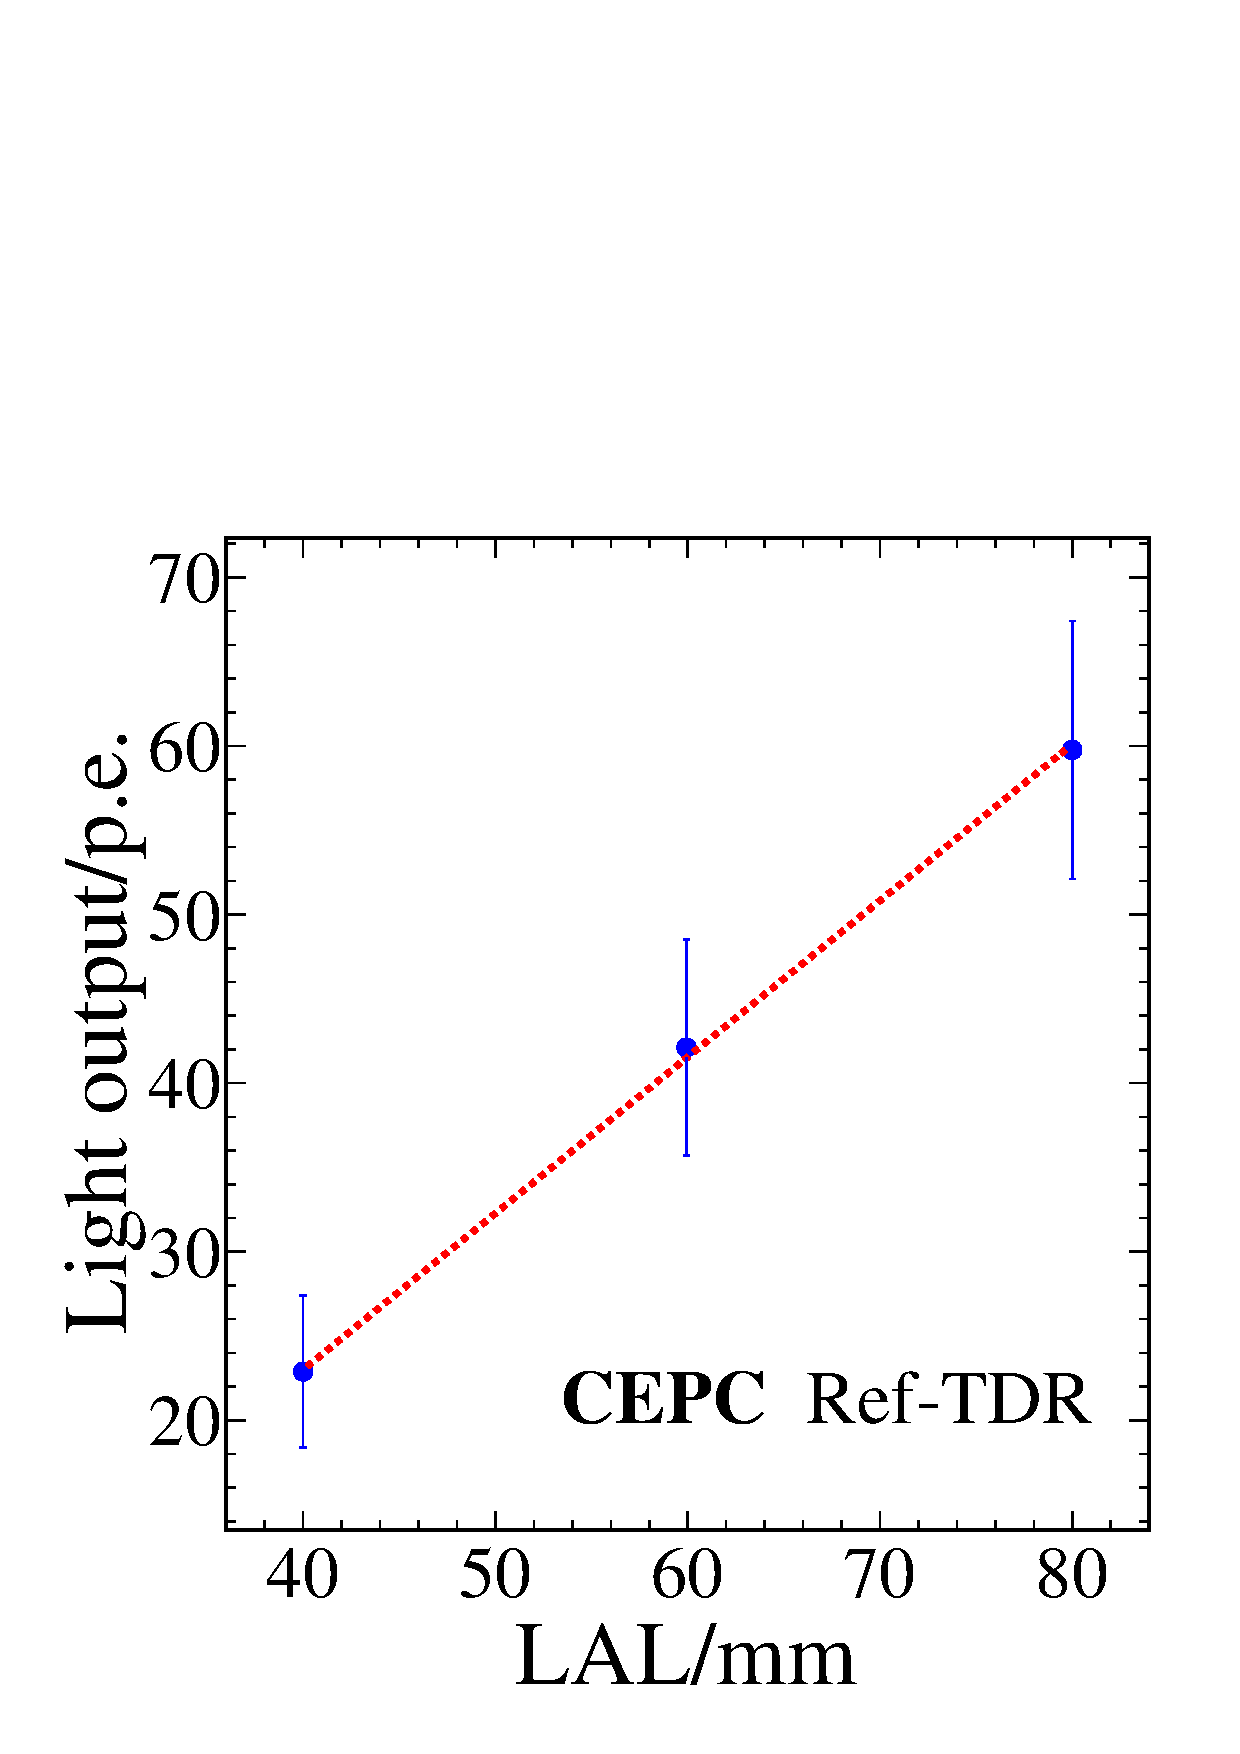
\includegraphics[width=\linewidth]{attenuation_fit.pdf}
  \caption{}
\end{subfigure}
\caption{(a)~Simulated light-output distribution of a GS cell with
\SI{60}{mm} attenuation length ($42.05\pm0.01$~\peMIP).
(b)~Fitted light-output MPV versus attenuation length.}
\label{fig:SiPM_MIPmap}
\end{figure}

Validation studies (Figure~\ref{fig:SiPM_SimValid}) show simulated
fast and slow scintillation components of \SI{96}{ns} and
\SI{1445}{ns}, somewhat longer than the measured reference values
of \SI{60}{ns} and \SI{500}{ns} (Table~\ref{tab:GS1}), and the
simulated single-muon light yield
(${\sim}\SI{42}{\peMIP}$) is lower than the measured cosmic-ray result
of ${\sim}\SI{64}{\peMIP}$ (Section~\ref{subsec:cellmeas}).
The optical simulation therefore plays a supporting role in the
baseline rationale rather than providing final experimental closure:
the current Geant4 optical model requires tuning against measured GFO
data, and this tuning is one of the immediate priorities of the
validation programme (Section~\ref{sec:discussion}).

\begin{figure}[htbp]
\centering
\begin{subfigure}{0.43\textwidth}
  \centering
  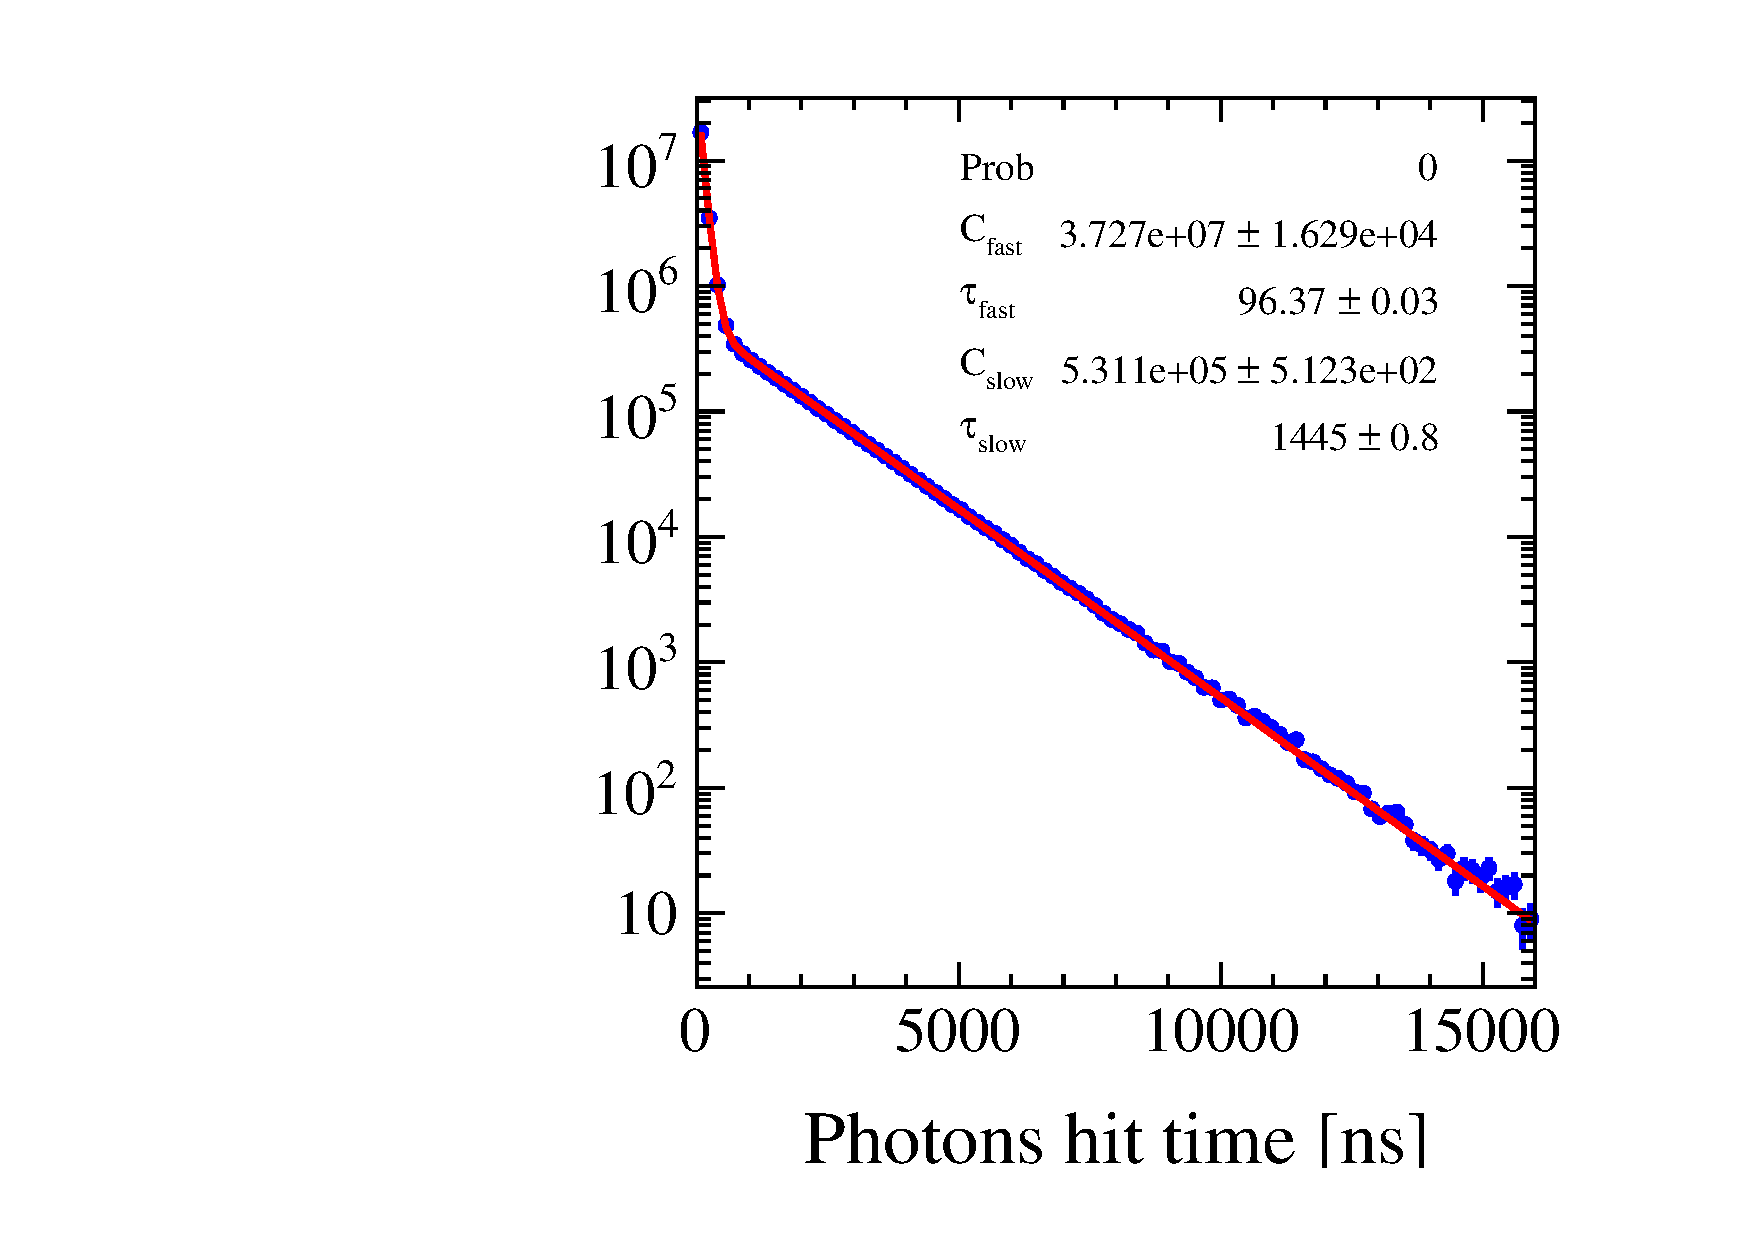
\includegraphics[width=\linewidth]{timeSpe.pdf}
  \caption{}
\end{subfigure}\hfill
\begin{subfigure}{0.38\textwidth}
  \centering
  \includegraphics[width=\linewidth]{Edp.pdf}
  \caption{}
\end{subfigure}
\caption{Simulation validation: (a)~scintillation-time distribution
(fast and slow components); (b)~muon deposited energy in a
\SI{10}{mm}-thick GS cell.}
\label{fig:SiPM_SimValid}
\end{figure}

%% ====================================================================
\section{Experimental characterisation of the baseline active unit}
\label{sec:expchar}
%% ====================================================================

The experimental evidence supporting the baseline active unit spans
four complementary measurement types.
The intrinsic light yield and optical response of the GFO glass
establish its suitability as the active medium.
Radiation-tolerance measurements confirm adequate performance under
CEPC-relevant doses.
Single-cell measurements with three independent probes---a
$^{137}$Cs source, cosmic-ray muons, and \SI{5}{GeV} electrons at
KEK---characterise the cell-level signal across the dynamic range of
interest.
Finally, initial tile-production studies address reproducibility and
quality control at batch scale.

%% --------------------------------------------------------------------
\subsection{Light yield and optical response}
\label{subsec:lightyield}
%% --------------------------------------------------------------------

Figure~\ref{fig:LargeGS} shows GFO glass cells of \cellsize under
natural and ultraviolet illumination.
Figure~\ref{fig:GS40}(a) shows the X-ray-excited luminescence (XEL)
and optical-transmission spectra of the GFO glass; the transmittance
in the visible range exceeds 80\%, with self-absorption observed near
the \SI{400}{nm} emission peak~\cite{SUI2025100878}.
Extensive $\gamma$-ray testing confirms that the GFO intrinsic light
yield consistently exceeds \SI{1000}{\phMeV}.
When measured with an XP2020 \SI{2}{inch} PMT, the GFO
photoelectron yield reaches approximately one-third that of BGO
crystals of identical dimensions~\cite{GS-5}
(Figure~\ref{fig:GS40}b).
Figure~\ref{fig:GS40}(c) shows the scintillation-decay profile under
$\gamma$-ray excitation: the slow-component decay time is below
\SI{500}{ns}, fully compatible with the high granularity and trigger
rate envisaged for the GS-HCAL.

Together these results establish the optical response required to
support the baseline cell: a light yield sufficient for
${\sim}60$~\peMIP readout, a transmittance compatible with bulk
photon transport across the cell, and a decay time compatible with
the baseline trigger window.

\begin{figure}[htbp]
\centering
\begin{subfigure}{0.40\textwidth}
  \centering
  \includegraphics[width=\linewidth]{GSN.pdf}
  \caption{}
\end{subfigure}\hfill
\begin{subfigure}{0.42\textwidth}
  \centering
  \includegraphics[width=\linewidth]{GSUV.pdf}
  \caption{}
\end{subfigure}
\caption{GFO glass cells of \cellsize under (a)~natural light and
(b)~ultraviolet illumination.}
\label{fig:LargeGS}
\end{figure}

\begin{figure}[htbp]
\centering
\begin{subfigure}{0.50\textwidth}
  \centering
  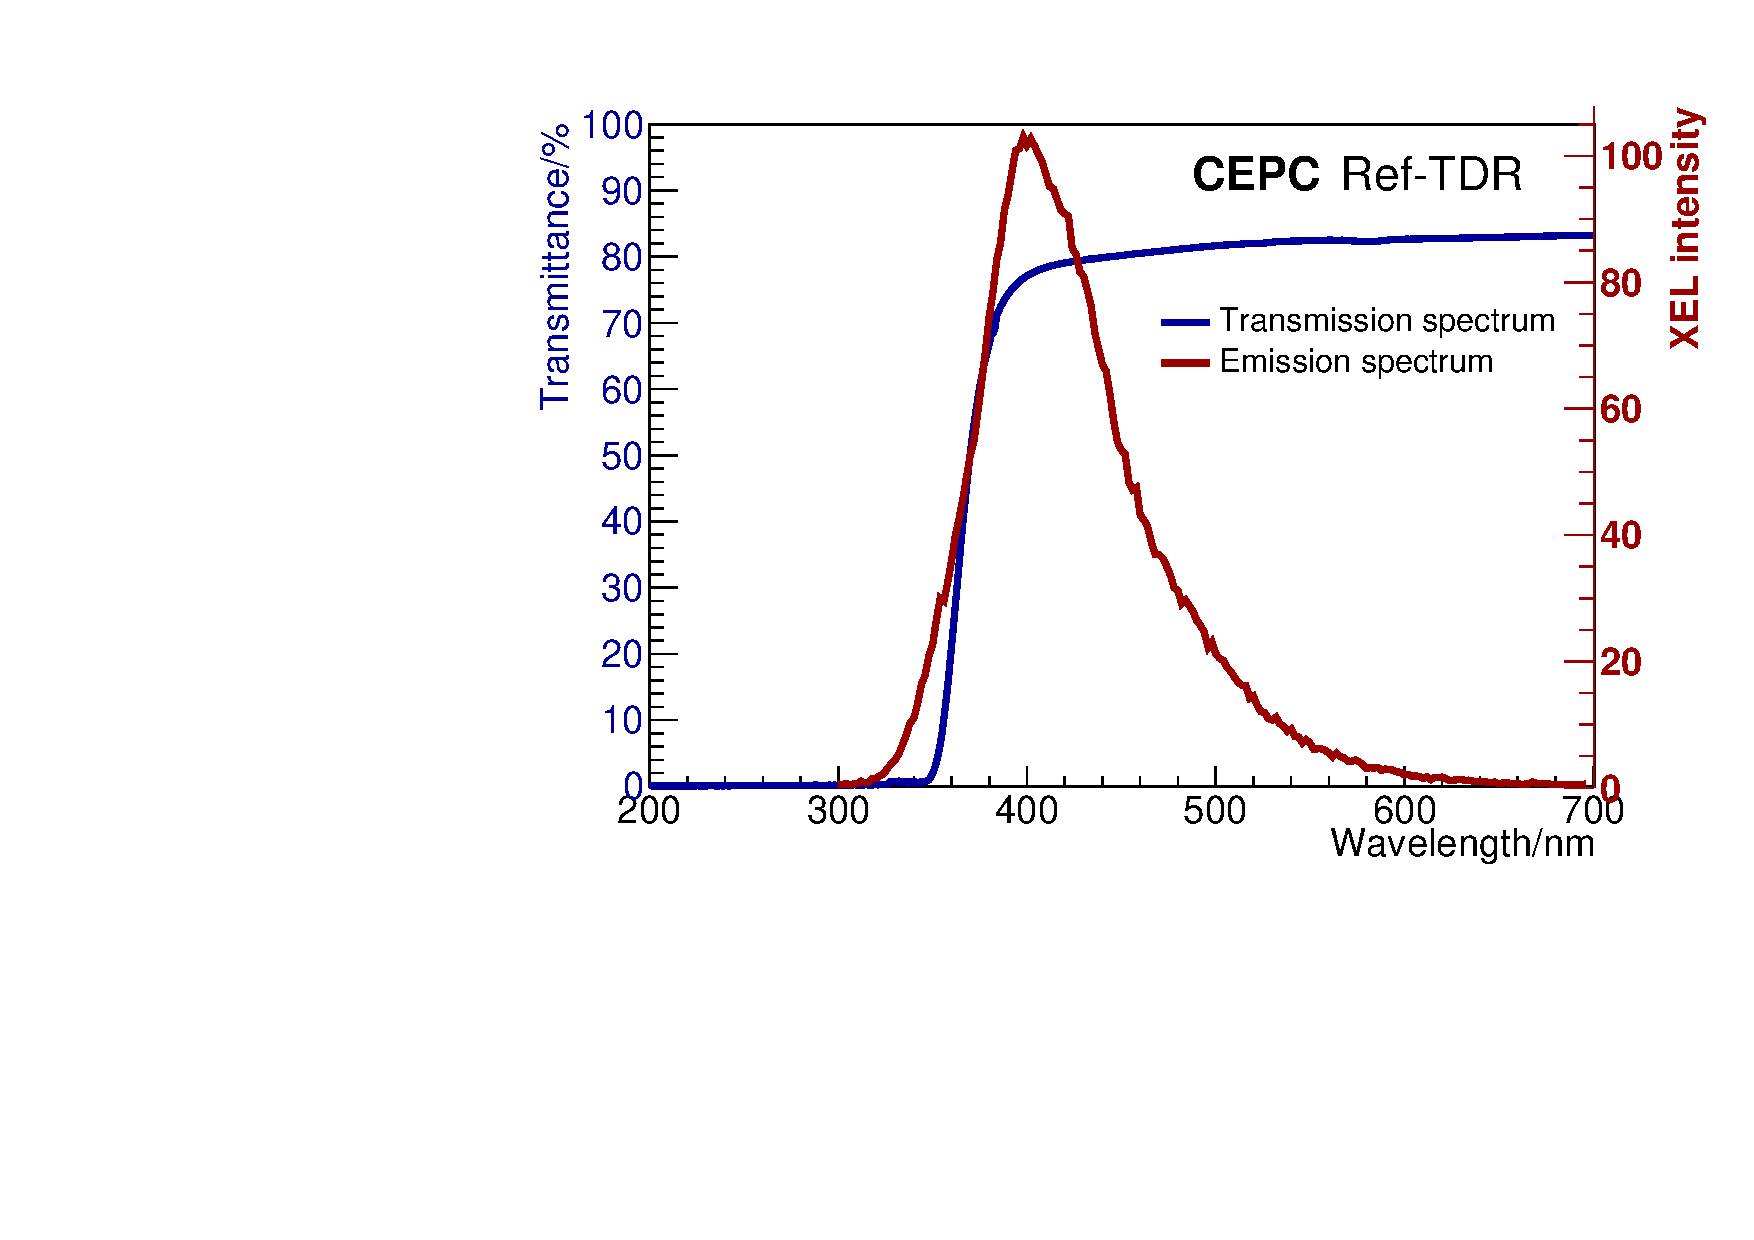
\includegraphics[width=\linewidth]{newGS40-A.pdf}
  \caption{}
  \label{fig:GS40-a}
\end{subfigure}

\vspace{0.3cm}

\begin{subfigure}{0.45\textwidth}
  \centering
  \includegraphics[width=\linewidth]{GS40-b.pdf}
  \caption{}
  \label{fig:GS40-b}
\end{subfigure}\hfill
\begin{subfigure}{0.45\textwidth}
  \centering
  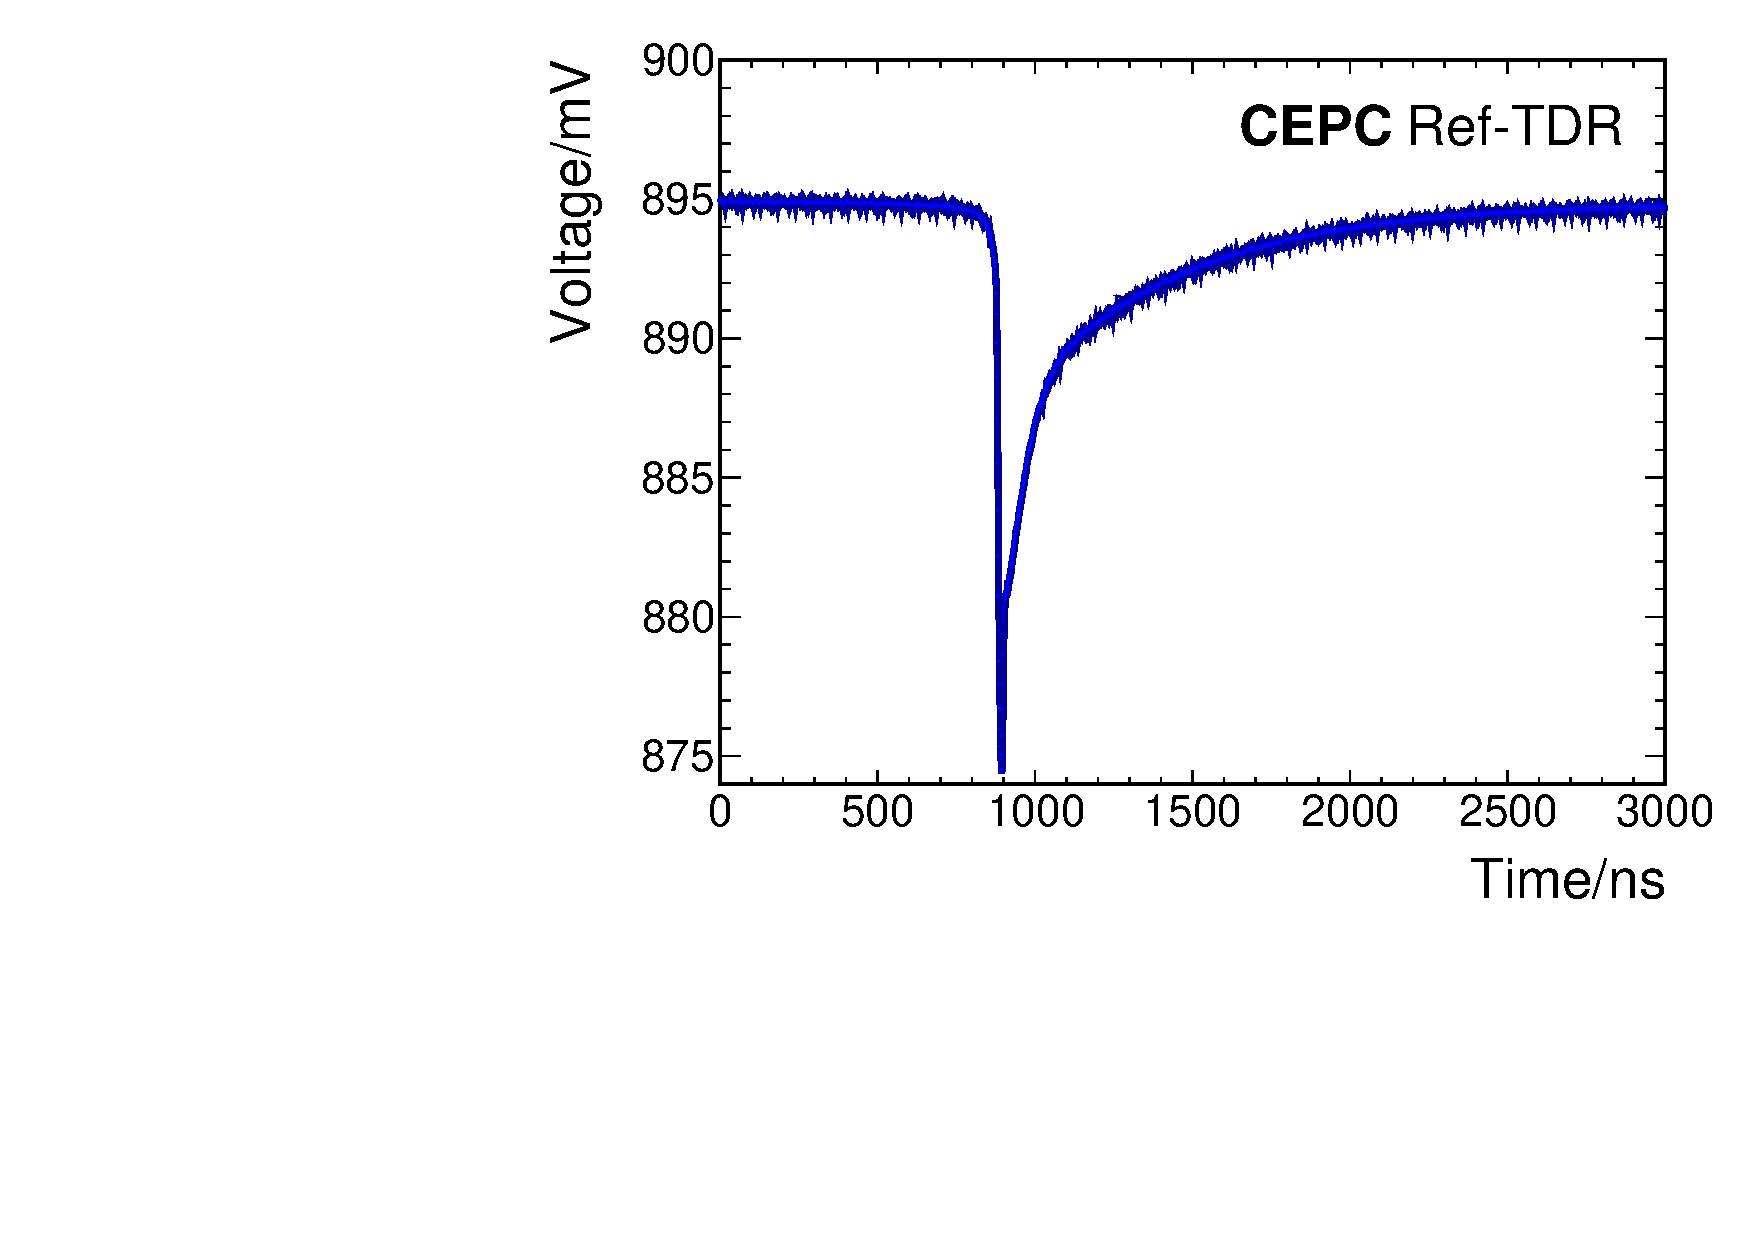
\includegraphics[width=\linewidth]{GS40-c.pdf}
  \caption{}
  \label{fig:GS40-c}
\end{subfigure}
\caption{(a)~Optical-transmission and XEL spectra of the GFO glass.
(b)~Energy spectra of GFO GS and BGO crystal of the same dimensions.
(c)~Scintillation decay curve of the GFO glass.}
\label{fig:GS40}
\end{figure}

%% --------------------------------------------------------------------
\subsection{Radiation tolerance under CEPC-relevant doses}
\label{subsec:radiation}
%% --------------------------------------------------------------------

Under the current CEPC operating plan, the accumulated radiation dose
reaches approximately \SI{40}{Gy} during the ten-year Higgs run at
$\mathcal{L}=8\times10^{34}$~cm$^{-2}$s$^{-1}$, and is estimated at
\SI{96}{Gy} per year during $Z$-pole operation at
$\mathcal{L}=192\times10^{34}$~cm$^{-2}$s$^{-1}$.
A dose benchmark of \SI{100}{Gy} therefore covers the practically
relevant operational range.

Figure~\ref{fig:gamma-irradiation} shows the relative light yield of
GFO glass as a function of $\gamma$-irradiation dose.
The retention exceeds 70\% at \SI{100}{Gy} (measured 71.2\%), and the
result is confirmed by proton-beam irradiation~\cite{YIN2026170869} at
the APEP facility~\cite{Liu:2022czi}.
These measurements demonstrate that the baseline active medium
preserves adequate optical response under CEPC-relevant doses.

\begin{figure}[htbp]
\centering
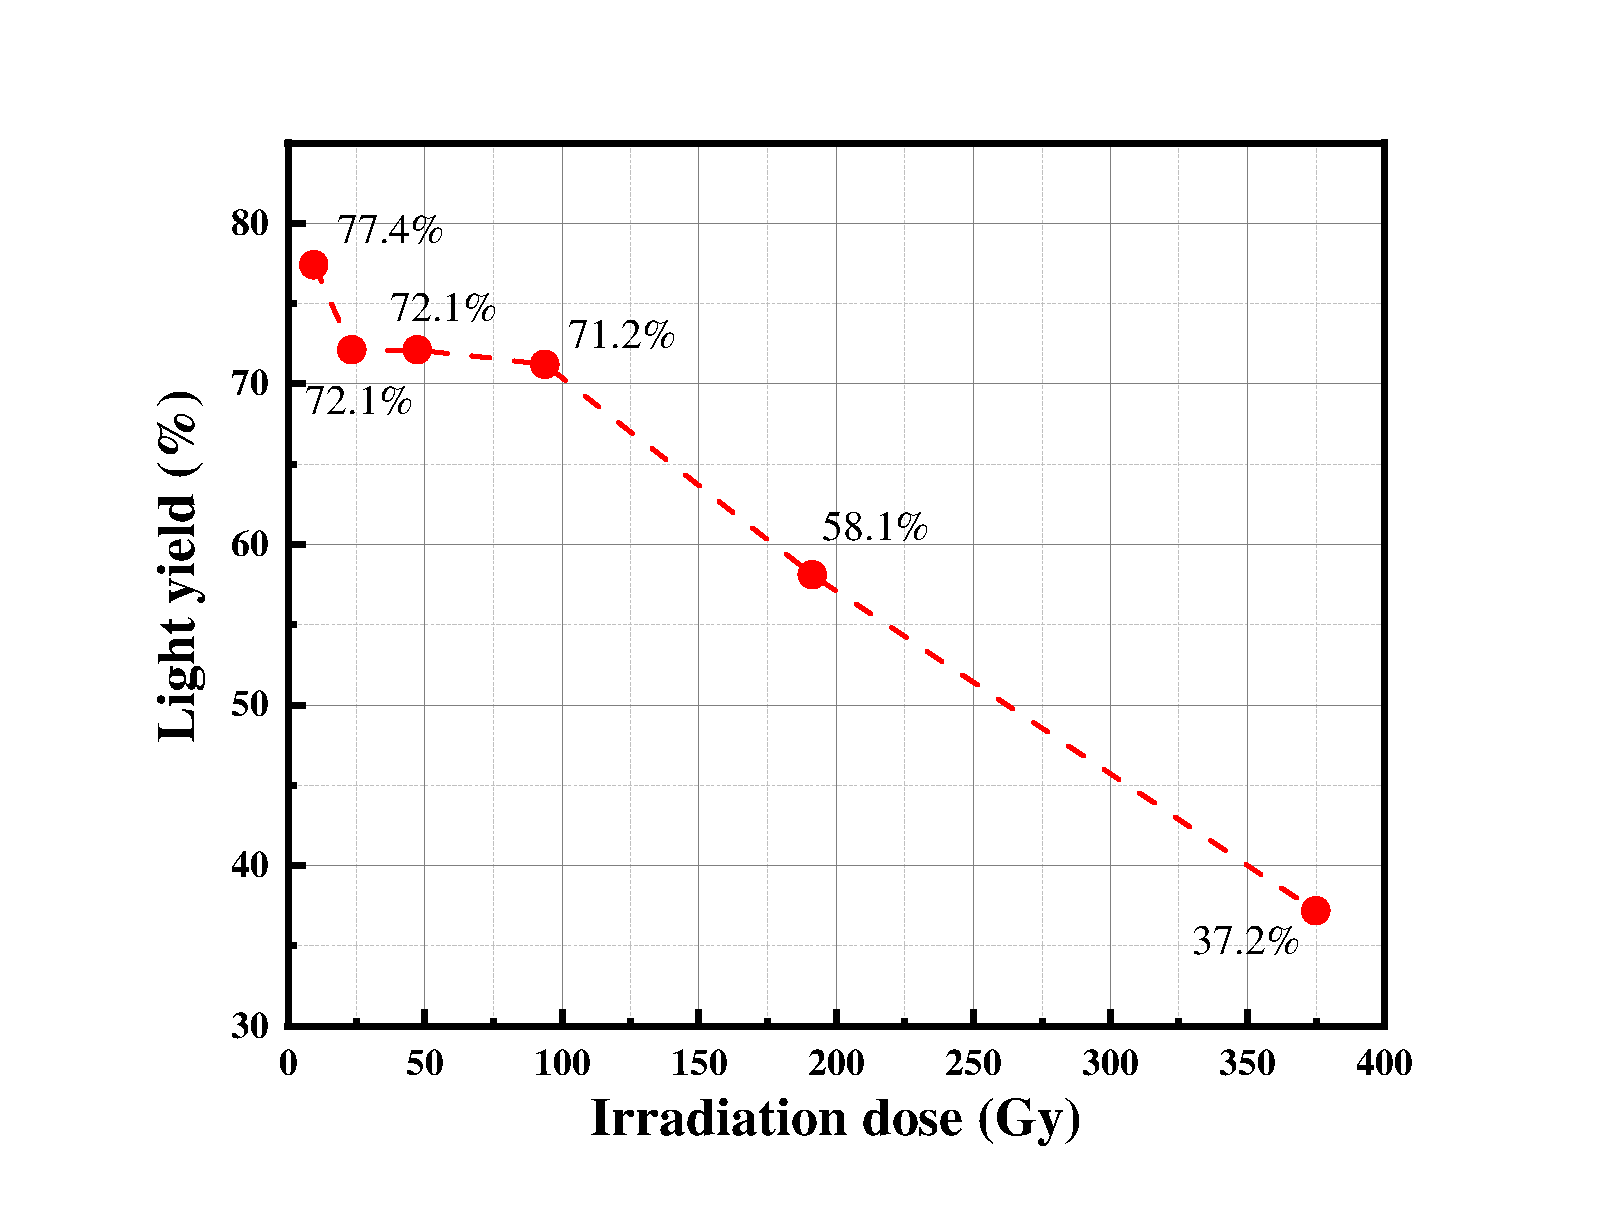
\includegraphics[width=0.60\linewidth]{LightYieldReductionGammaIrradiation.pdf}
\caption{Relative light yield of GFO glass as a function of
$\gamma$-irradiation dose.  At \SI{100}{Gy} the retention is 71.2\%.}
\label{fig:gamma-irradiation}
\end{figure}

%% --------------------------------------------------------------------
\subsection{Single-cell measurements with different probes}
\label{subsec:cellmeas}
%% --------------------------------------------------------------------

The effective light output of the \cellsize GS cell was evaluated in
three independent single-cell measurement campaigns using different
probes:
(i)~\SI{662}{keV} $\gamma$-rays from a $^{137}$Cs source;
(ii)~cosmic-ray muons with an expected energy deposition of
  \SI{7.7}{MeV/MIP};
(iii)~\SI{5}{GeV} electron beams at KEK.
In each case the SiPM was mounted at the cell centre on a readout
board with the interim pre-amplifier of Section~\ref{subsec:fee}.
Comparative tests of enhanced-specular-reflector (ESR) and Teflon
reflective films showed that Teflon provides approximately 20\%
higher effective reflectivity~\cite{Janecek:2012qit}, and all
measurements therefore employ Teflon wrapping.

\paragraph{$^{137}$Cs source.}
Using the HPK~S14160-3050HS SiPM (spectrum-weighted PDE~44.5\%), the
MPV for \SI{662}{keV} $\gamma$-rays is 12.9~p.e.;
scaled to a \SI{7.7}{MeV} MIP energy deposition this corresponds to an
equivalent light output of approximately 150~\peMIP.

\paragraph{Cosmic-ray muons.}
A trigger formed by two plastic-scintillator panels selects
through-going muons.
Using the HPK~S13360-3050PE SiPM (spectrum-weighted PDE~32.5\%), the
measured cell light output is $63.6\pm0.5$~\peMIP
(Figure~\ref{fig:SiPM_Celltest}b).

\paragraph{5~GeV electrons at KEK.}
A Landau fit to the electron spectrum measured with the
NDL~EQR20-11-3030 SiPM (spectrum-weighted PDE~42.5\%) yields an MPV of
$157.6\pm2.9$~\peMIP (Figure~\ref{fig:SiPM_Celltest}c).

\begin{figure}[htbp]
\centering
\begin{subfigure}{0.49\textwidth}
  \centering
  \includegraphics[width=\linewidth]{GS-SiPM-Cs137-Teflon.pdf}
  \caption{}
\end{subfigure}\hfill
\begin{subfigure}{0.49\textwidth}
  \centering
  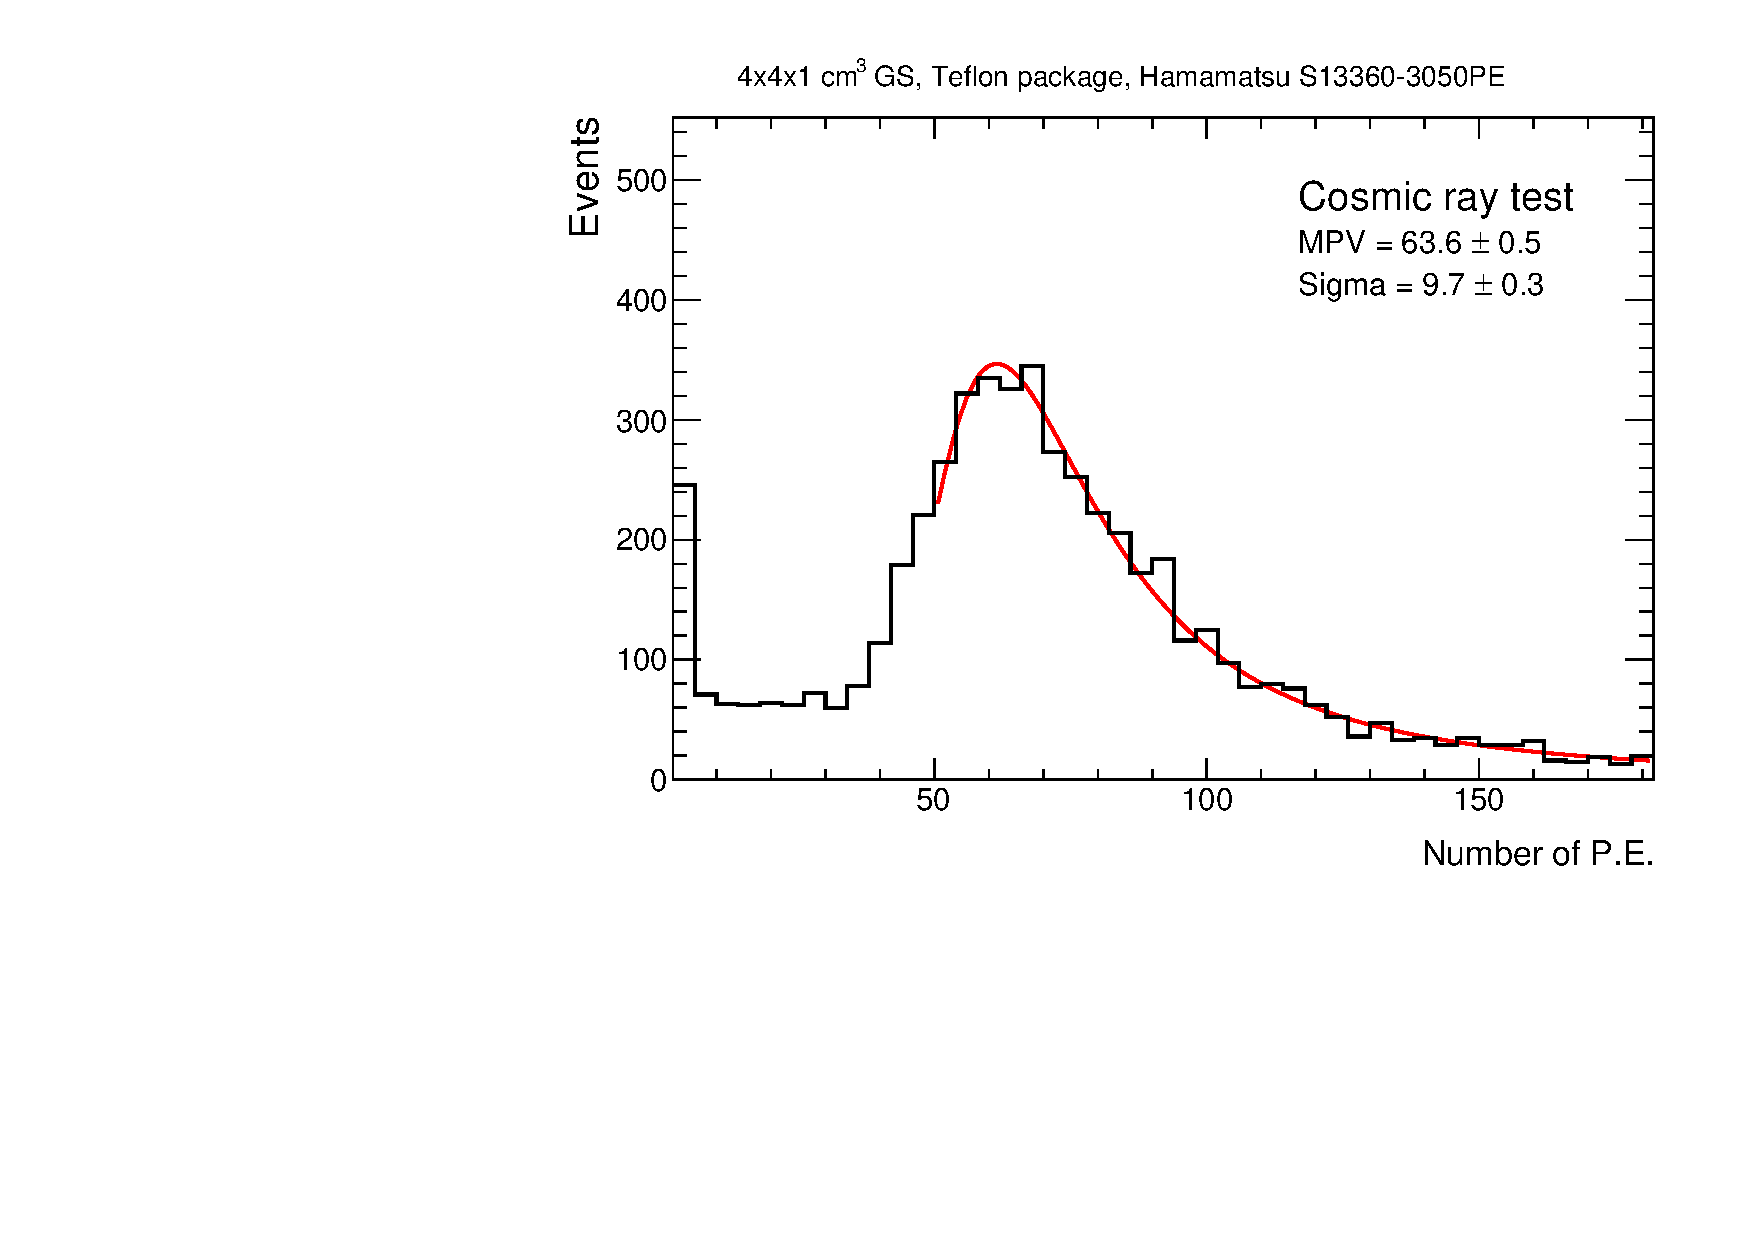
\includegraphics[width=\linewidth]{Cosmic_GSSiPM_SJTU_Teflon.pdf}
  \caption{}
\end{subfigure}

\vspace{0.3cm}

\begin{subfigure}{0.49\textwidth}
  \centering
  \includegraphics[width=\linewidth]{KEK_BeamTest_Electron.png}
  \caption{}
\end{subfigure}
\caption{Single-cell measurement results (\cellsize GS with SiPM
readout).
(a)~ADC spectrum with $^{137}$Cs source (HPK~S14160-3050HS).
(b)~Cosmic-ray test (HPK~S13360-3050PE): $63.6\pm0.5$~\peMIP.
(c)~Response to \SI{5}{GeV} electrons at KEK (NDL~EQR20-11-3030):
Landau-fit MPV $157.6\pm2.9$~\peMIP.}
\label{fig:SiPM_Celltest}
\end{figure}

\paragraph{Interpretation.}
The three probes are complementary rather than directly comparable.
The cosmic-ray muon provides the practical MIP-scale reference
(${\sim}\SI{7.7}{MeV}$ ionisation deposit in \SI{10}{mm} of GFO),
and it is this 64~\peMIP value that enters the baseline digitisation
model (Section~\ref{sec:simperf}).
The \SI{5}{GeV} electron is well above the GFO critical energy
($E_{c}\sim\SI{10}{MeV}$), so it deposits energy through an
electromagnetic shower whose local energy density exceeds that of a
MIP; the resulting 158~\peMIP is therefore higher than the
cosmic-ray value and is not a MIP signal.
The $^{137}$Cs result provides a low-energy check scaled by MIP
equivalence, which is also above the cosmic value.
Taken together the three probes consistently show that the GS cell
plus SiPM provides a signal amplitude well above the threshold
required by the SiPM DCR of Section~\ref{subsec:sipm}, establishing
the practical feasibility of the baseline active unit.
The residual discrepancy with the Geant4 optical simulation
(${\sim}\SI{42}{\peMIP}$) is discussed in
Section~\ref{subsec:optsim}.

%% --------------------------------------------------------------------
\subsection{Reproducibility and quality control}
\label{subsec:qc}
%% --------------------------------------------------------------------

Reproducible tile production is integral to the baseline concept,
because more than five million cells must deliver sufficiently uniform
light yield for PFA reconstruction.
To date approximately 290 tiles of \cellsize have been produced;
about 60\% of them meet the target intrinsic light yield of
\SI{1000}{\phMeV}.
The remaining tile-to-tile variation must be addressed through
two complementary channels: production-side optimisation aiming at a
higher fraction of tiles passing the target, and detector-side
calibration (Section~\ref{subsec:calibration}) that corrects residual
variations through MIP inter-calibration and LED monitoring.
An automated batch-testing platform is being developed to measure
light-yield uniformity, attenuation-length consistency, and
dimensional tolerances across large production batches, and a
production run of approximately \num{10000} tiles is planned to equip
the full-size prototype.
Mass-production optimisation of GFO tile yield and uniformity is
therefore recognised as one of the baseline's open engineering
items.

%% ====================================================================
\section{Simulation framework and projected detector performance}
\label{sec:simperf}
%% ====================================================================

The projected performance of the baseline detector is obtained from
full Geant4 digitisation-based simulation of the baseline geometry
within the CEPCSW framework.
These results are type-B evidence in the classification of
Section~\ref{subsec:why-baseline}: they establish that the baseline
configuration is consistent with the CEPC performance goals under the
current modelling assumptions, before full prototype beam validation.

%% --------------------------------------------------------------------
\subsection{Simulation setup and digitisation assumptions}
\label{subsec:simsetup}
%% --------------------------------------------------------------------

The simulation is performed with Geant4 within the CEPCSW
framework~\cite{CEPCStudyGroup:2018ghi}.
For single-hadron studies all inner sub-detectors are removed so that
the intrinsic GS-HCAL response is isolated; for physics-benchmark
studies the full reference-detector setup is used.
The digitisation model implements the following current modelling
assumptions:

\begin{itemize}
\item \textbf{Birks' constant:} a preliminary value
  $k_{B}=\SI{0.01}{cm/MeV}$, pending a dedicated heavy-ion
  measurement.
\item \textbf{Intrinsic light yield:} \SI{1500}{\phMeV}, giving a
  detected effective single-cell output of $\geq60$~\peMIP.
\item \textbf{Light attenuation length:} \SI{6}{cm}, taken from the
  current transmittance measurement.
\item \textbf{Readout threshold:} \SI{0.1}{MIP}, selected from a
  dedicated scan of its impact on the energy resolution.
\item \textbf{SiPM response and electronics effects:} included with
  the candidate SiPM parameters of Table~\ref{tab:SiPM-tab1}.
\end{itemize}

These are \emph{current modelling assumptions}: they are grounded in
measurements, but a subset of them (notably the Birks constant and
the optical-simulation light yield) is known to require further
tuning, and full experimental closure of the simulation chain is one
of the objectives of the prototype beam-test programme.

%% --------------------------------------------------------------------
\subsection{Single-hadron energy response}
\label{subsec:hadronres}
%% --------------------------------------------------------------------

The single-hadron energy resolution of the GS-HCAL is parametrised as
\begin{equation}
\label{eq:eres}
\frac{\sigma_{E}}{E} = \frac{a}{\sqrt{E}} \oplus b,
\end{equation}
where $a$ is the stochastic term and $b$ the constant term.
With the present digitisation model, and before full prototype beam
validation, the baseline detector configuration predicts
\begin{equation}
\frac{\sigma_{E}}{E} = \frac{29.8\%}{\sqrt{E\,[\text{GeV}]}}
\oplus 6.5\%,
\end{equation}
with energy non-linearity within 2\% (Figure~\ref{fig:Eres_HCAL_final};
\texttt{QGSP\_BERT} hadronic physics list).
The stochastic term is substantially below that of conventional
sampling HCALs (${\sim}60\%/\sqrt{E}\oplus3\%$), reflecting the high
active-medium density of the baseline.
The constant term is larger than the final CEPC target and is
dominated by longitudinal leakage in the $6\,\lambdaI$ design; this is
analysed in Section~\ref{subsec:constterm}.

\begin{figure}[htbp]
\centering
\begin{subfigure}{0.45\linewidth}
  \centering
  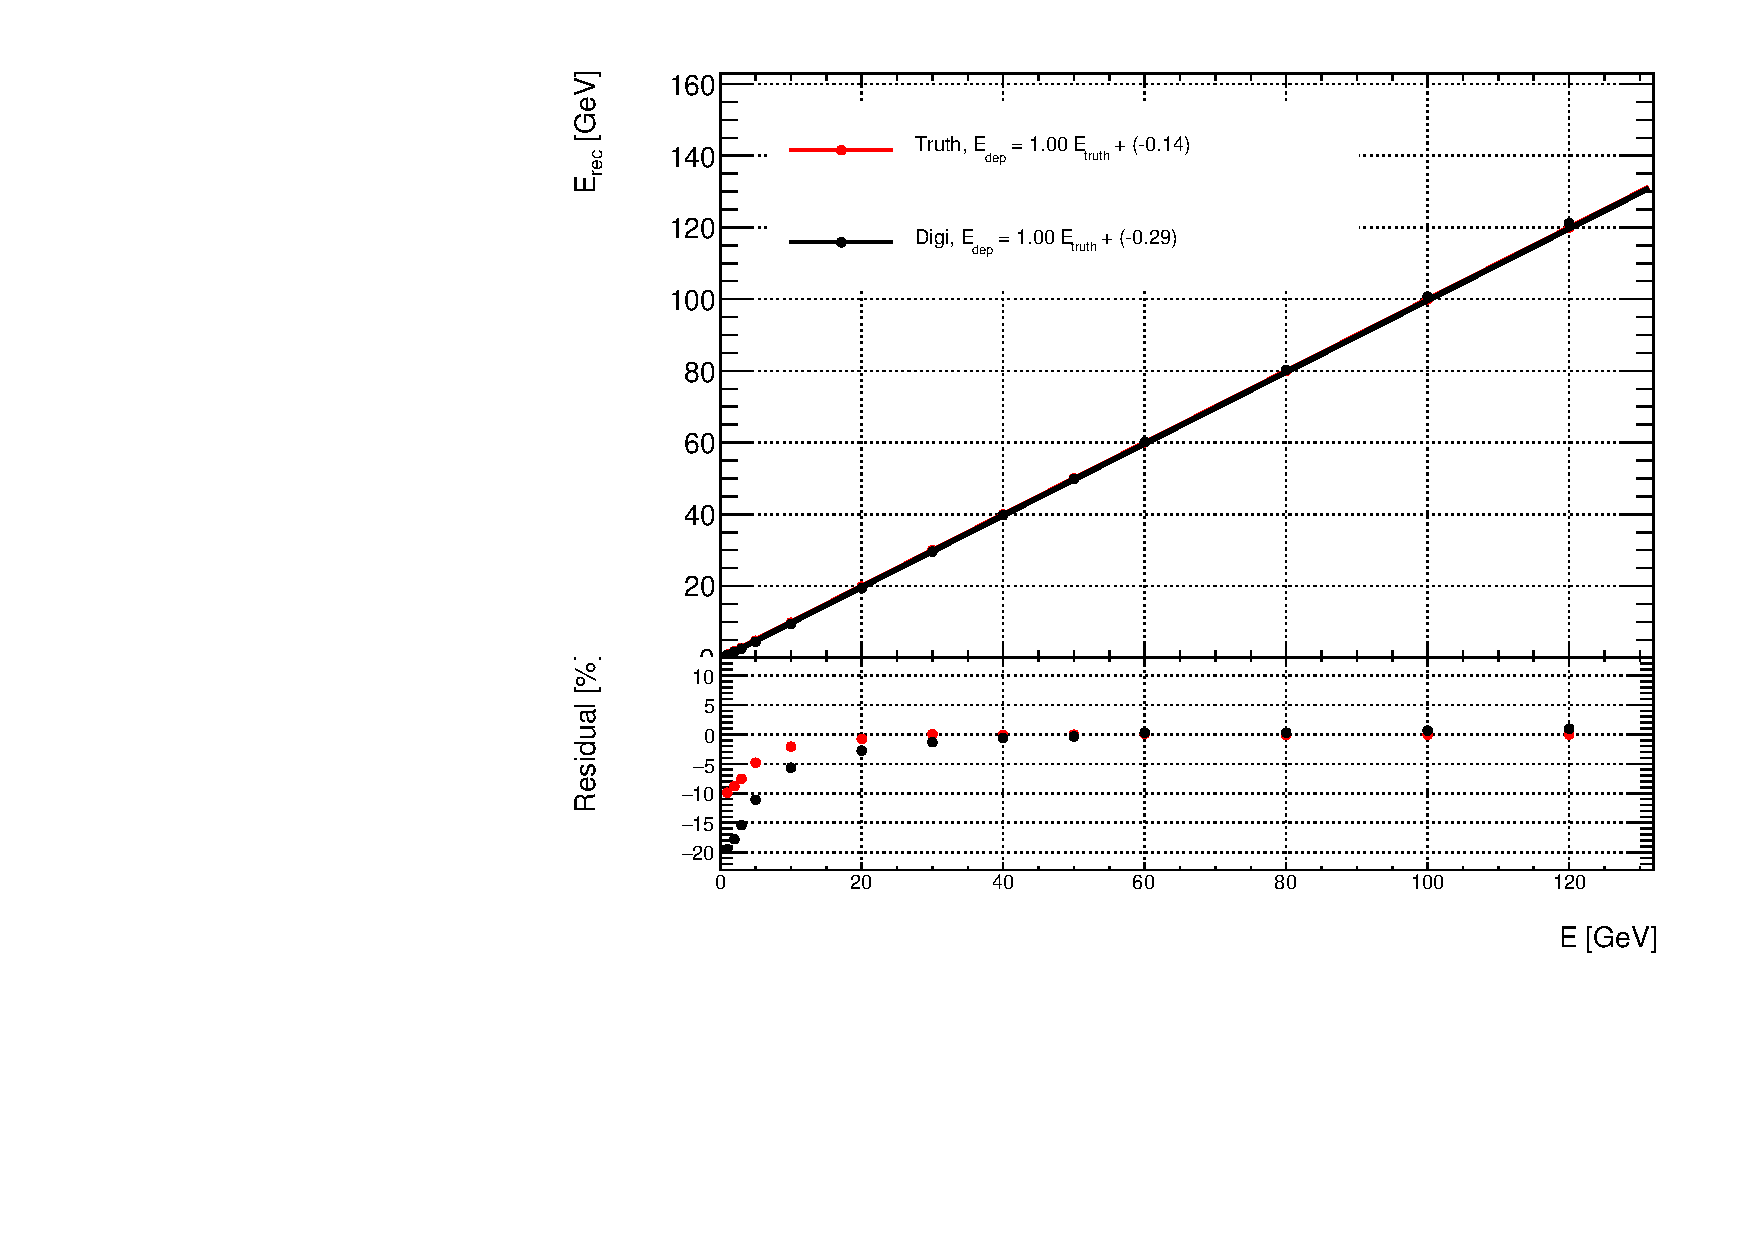
\includegraphics[width=\linewidth]{Elin_digi.pdf}
  \caption{}
\end{subfigure}\hfill
\begin{subfigure}{0.45\linewidth}
  \centering
  \includegraphics[width=\linewidth]{Eres_digi.pdf}
  \caption{}
\end{subfigure}
\caption{(a)~Energy linearity and (b)~energy resolution of the
baseline GS-HCAL from the full digitisation model.}
\label{fig:Eres_HCAL_final}
\end{figure}

In the CEPC collision environment
(Figure~\ref{fig:Ehad_CEPC}), more than 98\% of hadronic final-state
objects have energies below \SI{60}{GeV}, which is precisely the
regime in which the GS-HCAL stochastic term dominates and the
predicted resolution is best.

\begin{figure}[htbp]
\centering
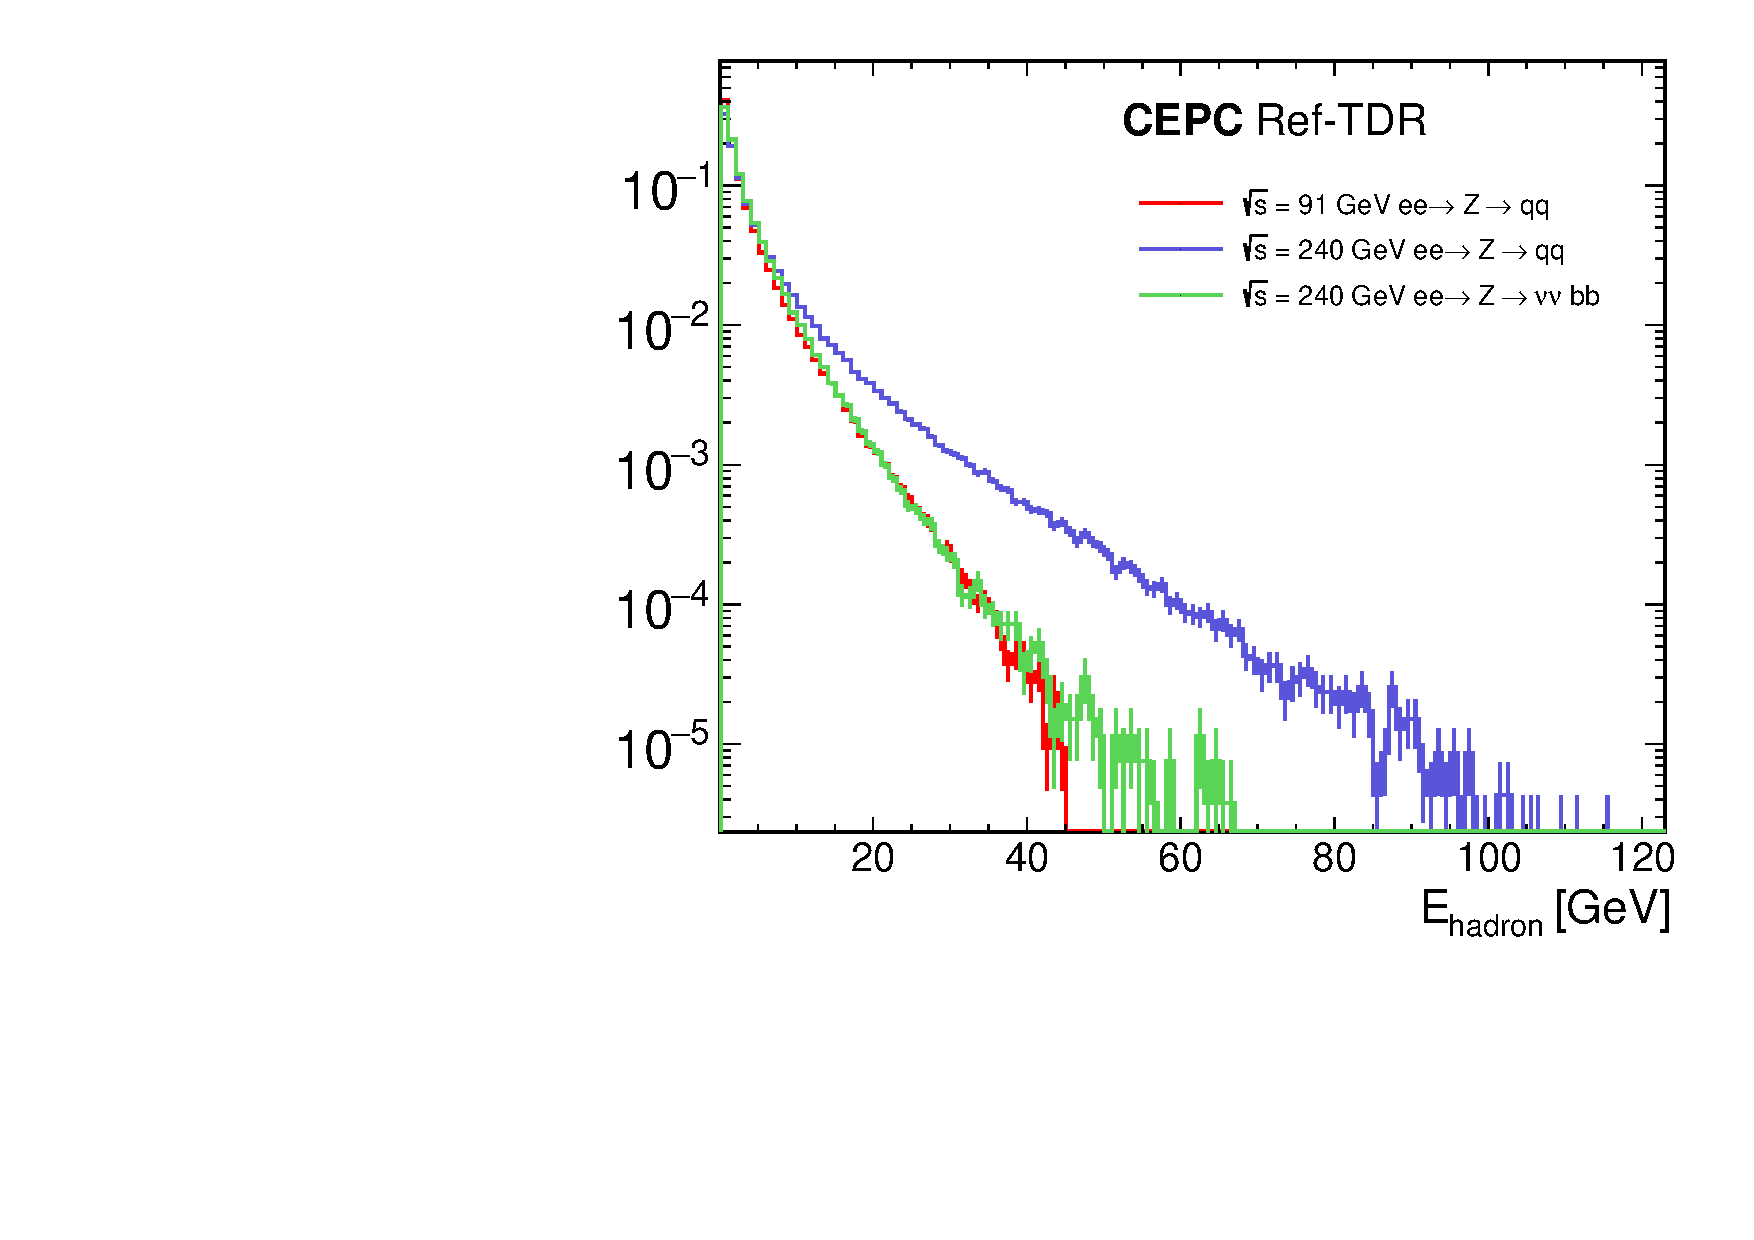
\includegraphics[width=0.50\linewidth]{Ehadrons.pdf}
\caption{Energy distribution of hadronic final-state objects in the
most energetic CEPC $e^{+}e^{-}$ processes.}
\label{fig:Ehad_CEPC}
\end{figure}

%% --------------------------------------------------------------------
\subsection{Sensitivity to key detector parameters}
\label{subsec:sensitivity}
%% --------------------------------------------------------------------

The sensitivity of the predicted single-hadron resolution to the
principal digitisation parameters is shown in
Figure~\ref{fig:Eres_vs_parameters} for
(a)~light output and readout threshold, (b)~attenuation length, and
(c)~Birks' constant.
These scans are not auxiliary: they are evidence that the baseline
parameter choices sit in a stable region of the resolution landscape.
In particular, the achieved cosmic-ray light output of
${\sim}\SI{64}{\peMIP}$ is well inside the saturated region of the
light-output/threshold scan, and the measured attenuation length of
${\sim}\SI{6}{cm}$ is likewise in the plateau of curve~(b).
The Birks-constant dependence quantifies the residual sensitivity
that will be reduced once a dedicated measurement is available.

\begin{figure}[htbp]
\centering
\begin{subfigure}{0.48\linewidth}
  \centering
  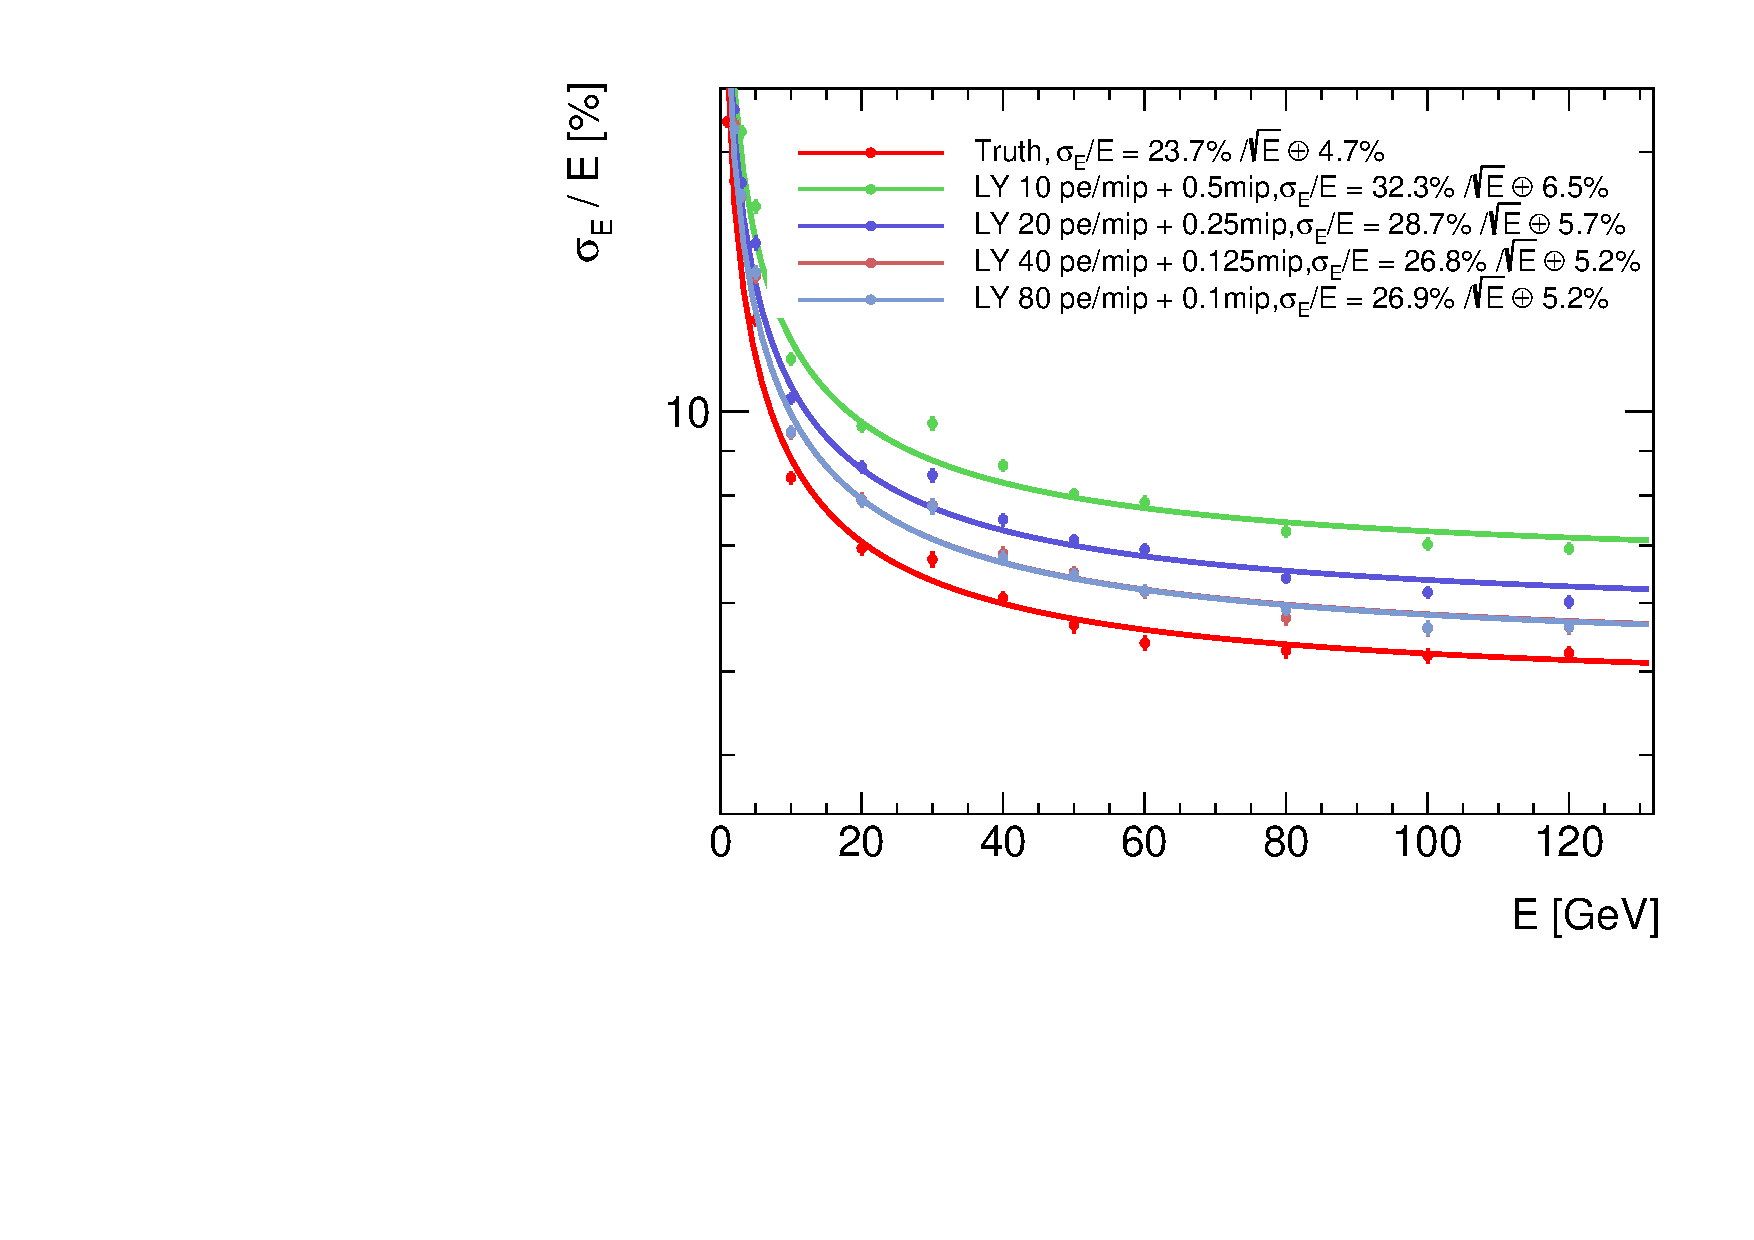
\includegraphics[width=\linewidth]{Eres_LYTh_Log.pdf}
  \caption{}
\end{subfigure}\hfill
\begin{subfigure}{0.48\linewidth}
  \centering
  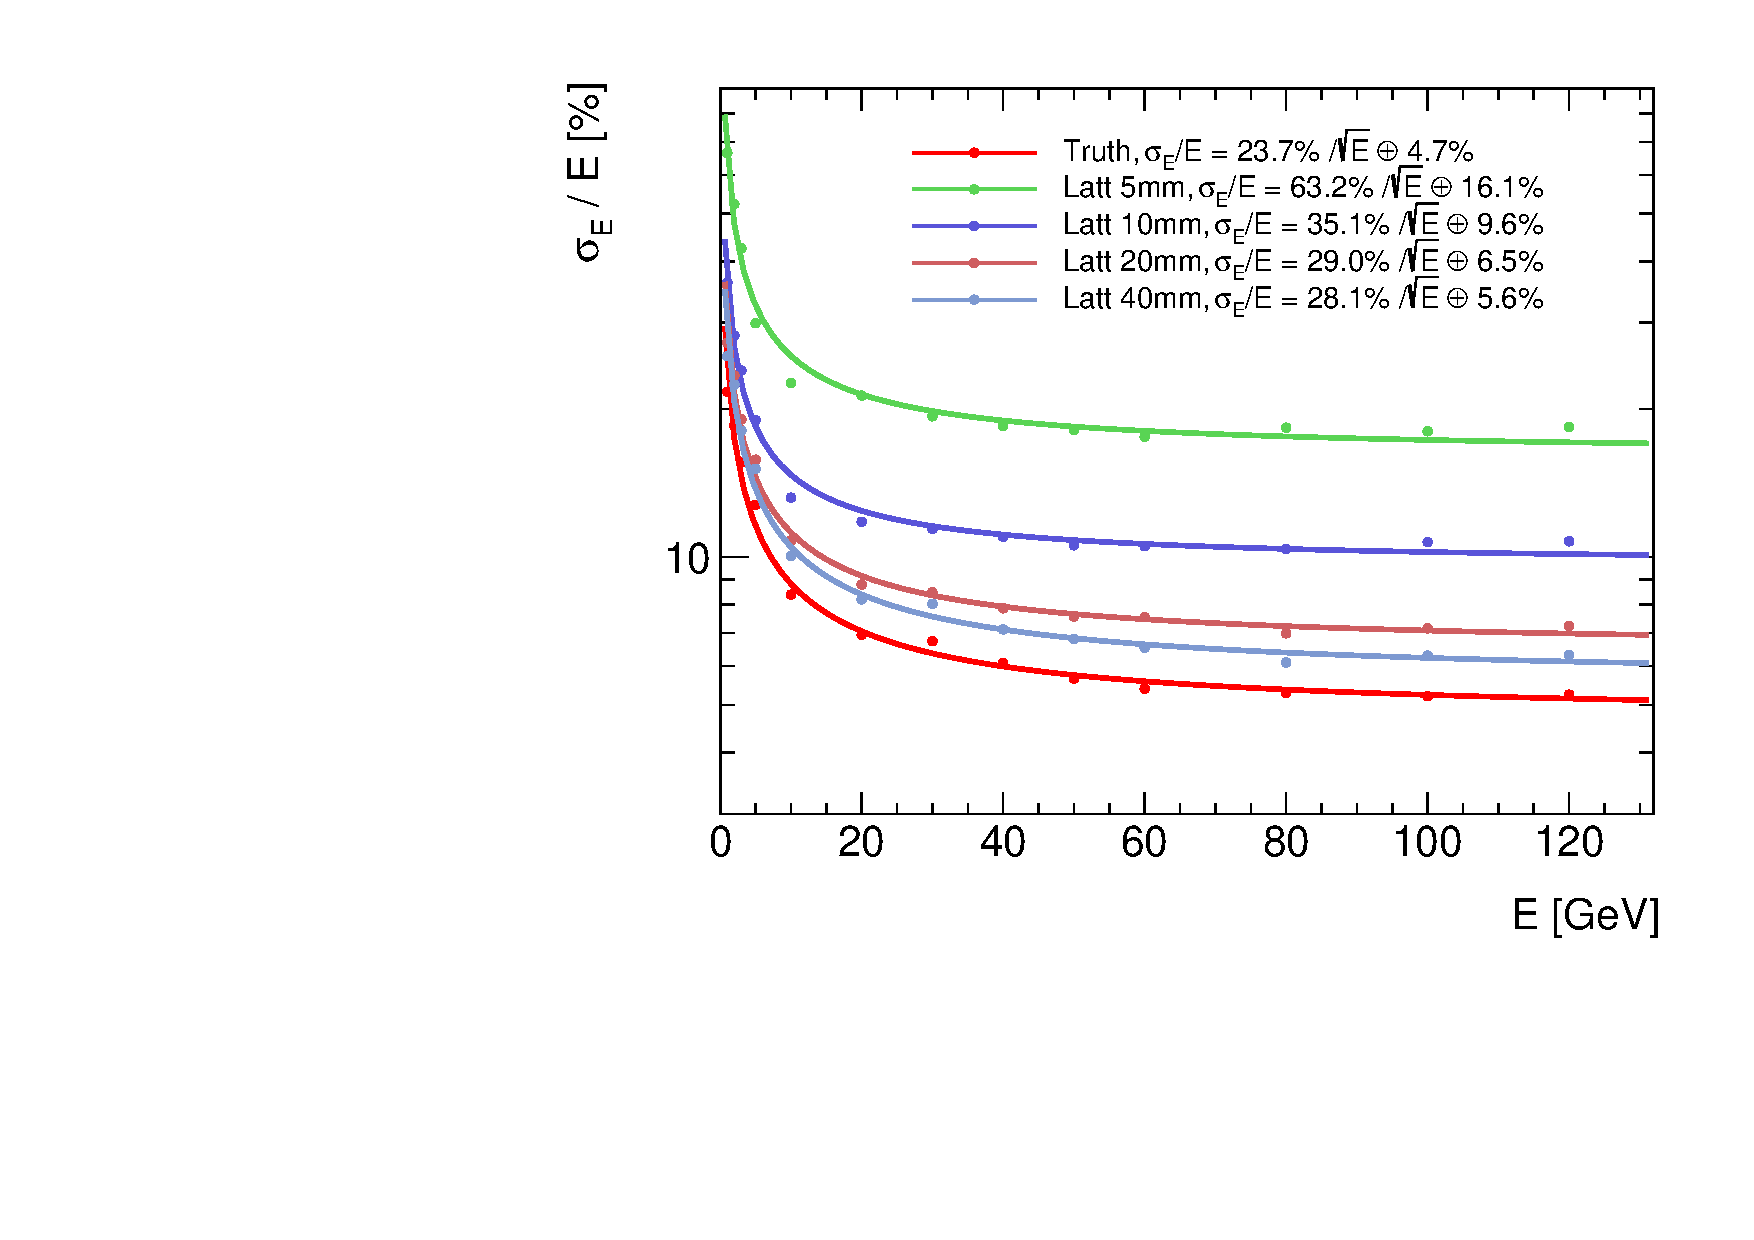
\includegraphics[width=\linewidth]{Eres_Latt_log.pdf}
  \caption{}
\end{subfigure}

\vspace{0.3cm}

\begin{subfigure}{0.48\linewidth}
  \centering
  \includegraphics[width=\linewidth]{ERes_Birks.pdf}
  \caption{}
\end{subfigure}
\caption{Simulated energy resolution as a function of
(a)~light output and readout threshold,
(b)~GS attenuation length, and
(c)~Birks' constant.}
\label{fig:Eres_vs_parameters}
\end{figure}

%% --------------------------------------------------------------------
\subsection{Origin of the constant term}
\label{subsec:constterm}
%% --------------------------------------------------------------------

The 6.5\% constant term obtained in Section~\ref{subsec:hadronres} is
interpreted as being dominated by longitudinal leakage in the
$6\,\lambdaI$ design.
Two independent studies support this interpretation.

First, increasing the standalone HCAL depth from 48~layers
($6\,\lambdaI$) to 80~layers ($10\,\lambdaI$) reduces the constant
term from 4.7\% to 2.9\% (Figure~\ref{fig:depth}), confirming that
leakage is the dominant source.

Second, the upstream environment of the full reference detector is
expected to mitigate this effect.
The BGO ECAL contributes ${\approx}1.2\,\lambdaI$ of upstream
material, causing approximately 70\% of hadrons to initiate showers
before entering the HCAL.
Requiring the first hadronic interaction to occur within the first two
GS-HCAL layers ($0.25\,\lambdaI$) already reduces the constant term to
approximately 3\%, consistent with the PS-HCAL prototype
result~\cite{CALICE:2010fpb,Liu:2025hgf}.

This analysis identifies leakage rather than the intrinsic GS-HCAL
response as the origin of the current constant term; it does not
itself close the constant term, but it shows that the baseline
architecture is compatible with the target 3--4\% BMR.

\begin{figure}[htbp]
\centering
\begin{subfigure}{0.48\textwidth}
  \centering
  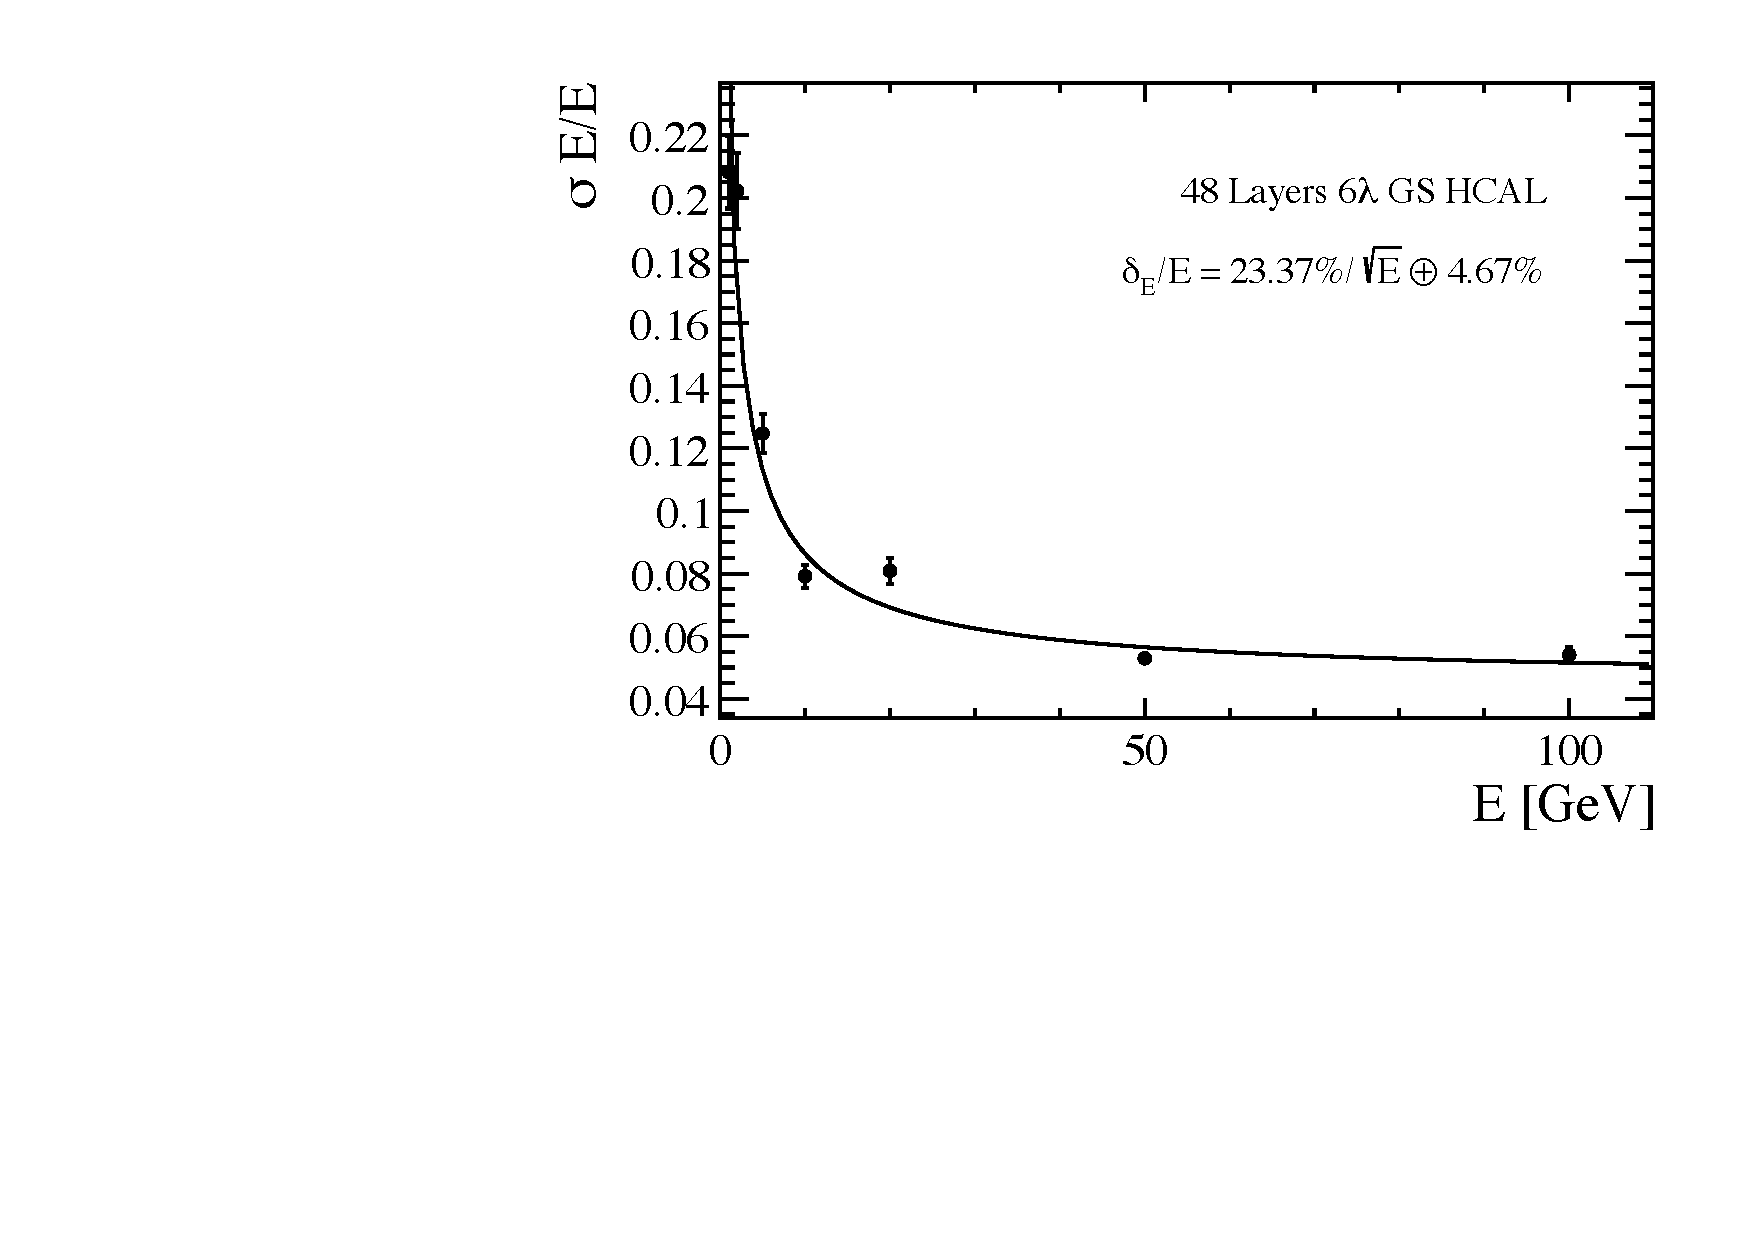
\includegraphics[width=\linewidth]{const_gs_6lambda.pdf}
  \caption{}
\end{subfigure}\hfill
\begin{subfigure}{0.48\textwidth}
  \centering
  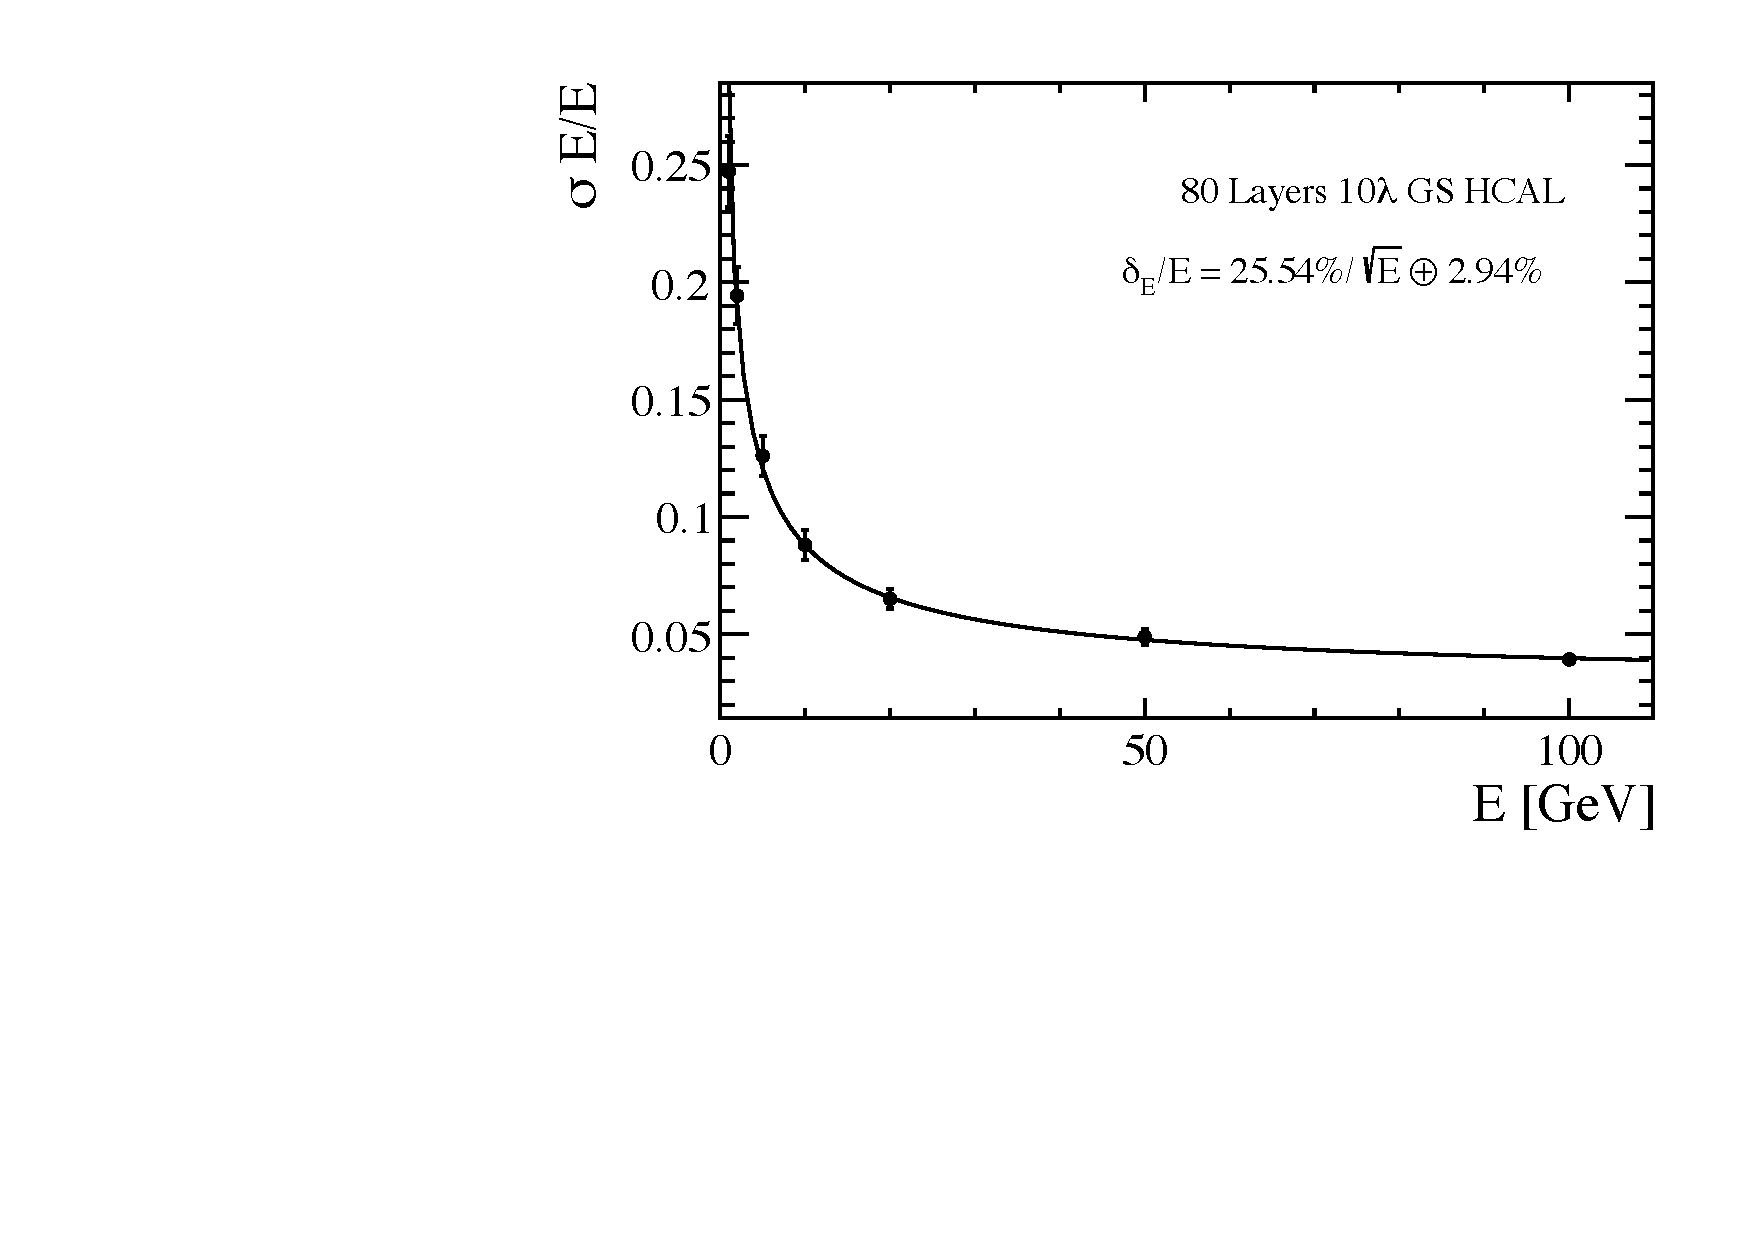
\includegraphics[width=\linewidth]{const_gs_10lambda.pdf}
  \caption{}
\end{subfigure}
\caption{Energy-resolution distributions for two GS-HCAL depths.
(a)~$6\,\lambdaI$ (48~layers): pronounced high-energy tail.
(b)~$10\,\lambdaI$ (80~layers): constant term reduced from 4.7\%
to 2.9\%.}
\label{fig:depth}
\end{figure}

%% --------------------------------------------------------------------
\subsection{Electron--hadron response}
\label{subsec:eresponse}
%% --------------------------------------------------------------------

The baseline calorimeter response to electrons and to different
hadron species is studied with full Geant4 simulation of the
standalone GS-HCAL\@.
Fitting $E_{\mathrm{true}}=C\times S_{\mathrm{HCAL}}$ separately for
each species gives the calibration slopes of
Table~\ref{tab:eoverh_hcal}.
The empirical hadron-to-electron response ratio
$C_{\mathrm{hadron}}/C_{e}$ of 1.09--1.14 is consistent with a
non-compensating sampling calorimeter~\cite{Akchurin:2012zz}.
The empirical ratio must be distinguished from the intrinsic
compensation ratio $e/h$ of the shower physics, which is the actual
figure of merit for the constant term; the intrinsic $e/h$ has not
yet been extracted, and its extraction through shower-component
decomposition is part of the open-item list of
Section~\ref{sec:discussion}.
Software-compensation and energy-weighting techniques
exploiting this intrinsic $e/h$ are expected to reduce the constant
term below~3\%.

\begin{table}[htbp]
\centering
\caption{Calibration slopes $C$ and electron--hadron response ratios
$C_{\mathrm{hadron}}/C_{e}$ for the baseline GS-HCAL\@.}
\label{tab:eoverh_hcal}
\begin{tabular}{lcc}
\toprule
Particle & $C$ (slope) & $C_{\mathrm{hadron}}/C_{e}$ \\
\midrule
Electron  & $2.94\pm0.01$ & ---            \\
$\pi^{-}$ & $3.20\pm0.05$ & $1.09\pm0.02$ \\
$K^{+}$   & $3.28\pm0.05$ & $1.12\pm0.02$ \\
Neutron   & $3.35\pm0.07$ & $1.14\pm0.02$ \\
Proton    & $3.36\pm0.07$ & $1.14\pm0.02$ \\
\bottomrule
\end{tabular}
\end{table}

%% --------------------------------------------------------------------
\subsection{Physics benchmark: $H\to gg$}
\label{subsec:physperf}
%% --------------------------------------------------------------------

The physics-benchmark performance of the baseline is evaluated through
PFA reconstruction of $H\to gg$, the most HCAL-sensitive of the
standard Higgs-dijet benchmarks.
Events are generated with \textsc{Whizard}\,v1.9.5~\cite{Kilian:2007gr,
Moretti:2001zz} and propagated through the full reference-detector
simulation with Geant4\,v11.2 in the CEPCSW framework.
Figure~\ref{fig:ch08_BMR} shows the reconstructed dijet invariant
mass; the fitted Higgs-boson mass is
$126.32\pm0.04$~GeV/$c^{2}$ with
$\sigma(m_{jj})=4.90\pm0.04$~GeV/$c^{2}$, corresponding to a boson
mass resolution (BMR) of 3.88\%, within the CEPC target of 3--4\%.

This result is detector-level strong evidence that the baseline
concept is compatible with the CEPC physics goals, but it is
simulation-based and does not replace prototype beam validation.

\begin{figure}[htbp]
\centering
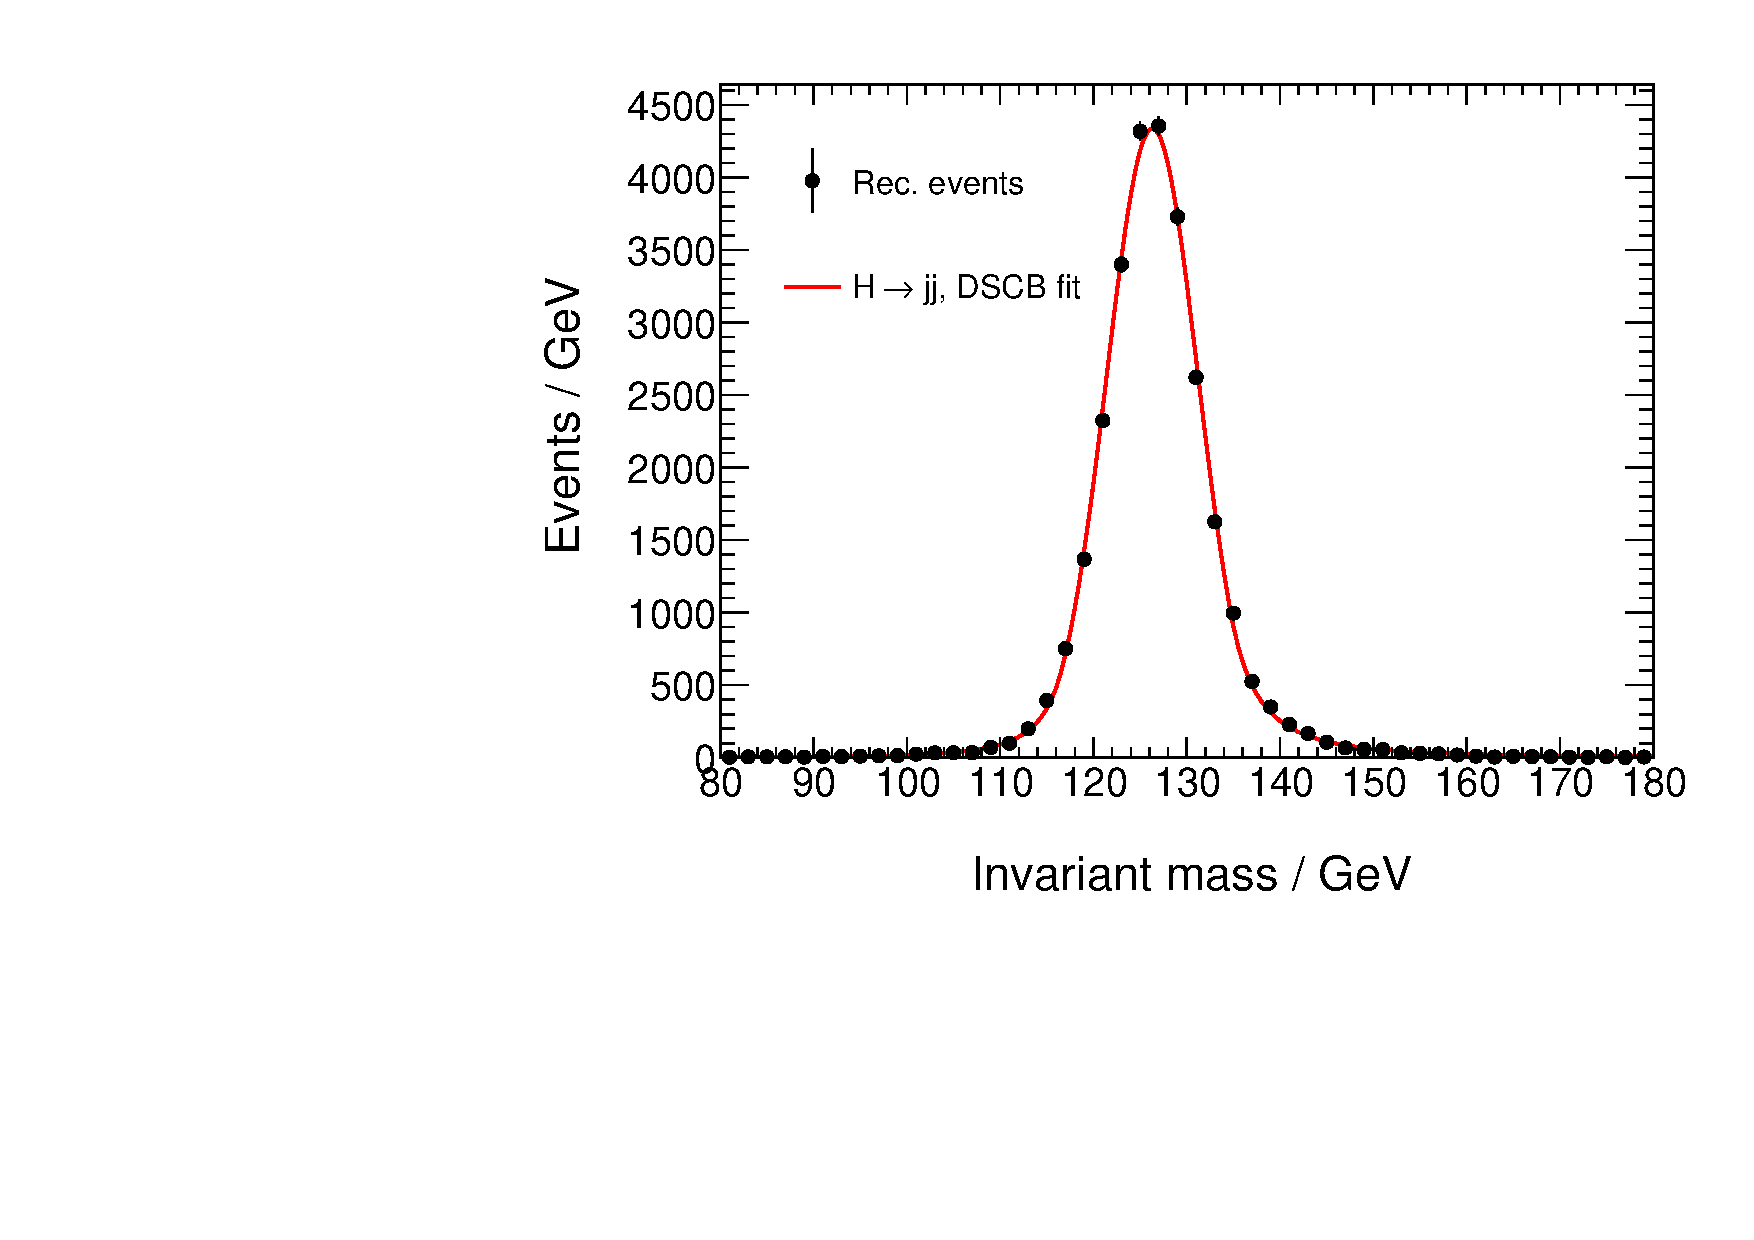
\includegraphics[width=0.60\linewidth]{Fig8.9_BMR.pdf}
\caption{Reconstructed dijet invariant mass for $H\to gg$ with the
baseline GS-HCAL\@.
Fitted mass: $126.32\pm0.04$~GeV/$c^{2}$;
$\sigma(m_{jj})=4.90\pm0.04$~GeV/$c^{2}$; BMR~=~3.88\%.}
\label{fig:ch08_BMR}
\end{figure}

%% ====================================================================
\section{Mechanical feasibility, calibration strategy, and prototype
validation}
\label{sec:feasibility}
%% ====================================================================

Establishing the technical basis of the baseline requires not only
material and simulation evidence but also demonstrated detector-scale
mechanical viability, a defined calibration architecture, and a
concrete prototype beam-test plan.
These three aspects are presented together because they jointly
determine whether the baseline can be realised at full scale.

%% --------------------------------------------------------------------
\subsection{Mechanical feasibility at detector scale}
\label{subsec:mechanics}
%% --------------------------------------------------------------------

Finite-element analysis of the full barrel+endcap structure supports
the detector-scale mechanical viability of the baseline concept.
The critical load is the \SI{135}{t} BGO ECAL supported by the
barrel while the layer-to-layer alignment required by PFA is
preserved.
Figure~\ref{fig:deformation_barrel} shows the deformation distribution
with and without ECAL loading.

\begin{figure}[htbp]
\centering
\begin{subfigure}{0.80\linewidth}
  \centering
  \includegraphics[width=\linewidth]{1.7.1.3.3-3.png}
  \caption{}
\end{subfigure}

\vspace{0.3cm}

\begin{subfigure}{0.80\linewidth}
  \centering
  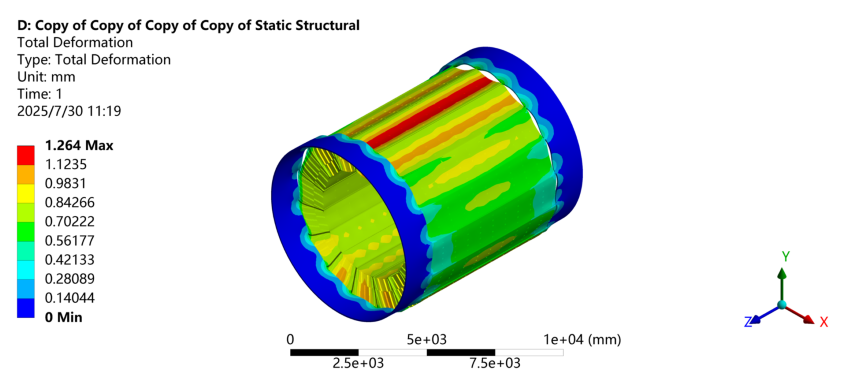
\includegraphics[width=\linewidth]{1.7.1.3.3-2.png}
  \caption{}
\end{subfigure}
\caption{Deformation distribution of the GS-HCAL barrel (a)~without
and (b)~with ECAL loading.}
\label{fig:deformation_barrel}
\end{figure}

During assembly the maximum deformation remains below \SI{0.66}{mm}
and the localised stress below \SI{190}{MPa}, well under the yield
strength.
Under the full ECAL load, peak stresses reach \SI{371}{MPa} at
specific connection points; these critical areas employ titanium-alloy
(TC4) components with safety factors above~2.2, while the bulk of the
structure is stainless steel.
Layer-to-layer deformation differences remain below \SI{0.2}{mm}
(within the \SI{2.4}{mm} gasket range), intra-layer deformations are
below \SI{0.5}{mm} inducing only \SI{20}{MPa} stress in the GS cells,
and the scintillator boxes withstand \SI{0.5}{mm} bending with a
safety factor above three.
Taken together, these results support the detector-scale mechanical
viability of the baseline concept; they are type-B evidence on the
engineering side, complementing the simulation-based detector
performance of Section~\ref{sec:simperf}.

%% --------------------------------------------------------------------
\subsection{Calibration strategy as part of the baseline architecture}
\label{subsec:calibration}
%% --------------------------------------------------------------------

Calibration is integral to the baseline concept rather than an
auxiliary activity: with 5.22~million channels and tile-to-tile light
yield variations, no operating point of the detector is reachable
without a well-defined calibration architecture.
The baseline therefore incorporates two complementary calibration
layers, physics-process calibration and hardware calibration.

\paragraph{Physics-process calibration.}
Global calibration exploits MIP signals from
$e^{+}e^{-}\to Z\to\mu^{+}\mu^{-}$ events.
At design luminosity the process rate is \SI{584}{Hz}, corresponding
to approximately 47~events per hour within a $\Delta\phi\times
\Delta\!\cos\theta=0.018\times0.018$ acceptance window matched to
one central-barrel HCAL cell (Figure~\ref{fig:kinematic_mumu}).
Bi-weekly \SI{16}{h/day} calibration runs accumulate
$4.71\times10^{8}$ di-muon events, yielding ${\sim}1\%$ statistical
precision per cell.
In addition, $e^{+}e^{-}\to Z\to q\bar{q}$ (Figure~\ref{fig:kinematic_zjj})
provides resonant dijets for combined ECAL+HCAL response
calibration through the reconstructed $m_{jj}$, and hadronic $\tau$
decays in $Z\to\tau^{+}\tau^{-}$ provide complementary $E/p$
monitoring over time.

\begin{figure}[htbp]
\centering
\begin{subfigure}{0.32\textwidth}
  \centering
  \includegraphics[width=\linewidth]{Fig8_mumu_cosTheta.pdf}
  \caption{}
\end{subfigure}\hfill
\begin{subfigure}{0.32\textwidth}
  \centering
  \includegraphics[width=\linewidth]{Fig8_mumu_phi.pdf}
  \caption{}
\end{subfigure}\hfill
\begin{subfigure}{0.32\textwidth}
  \centering
  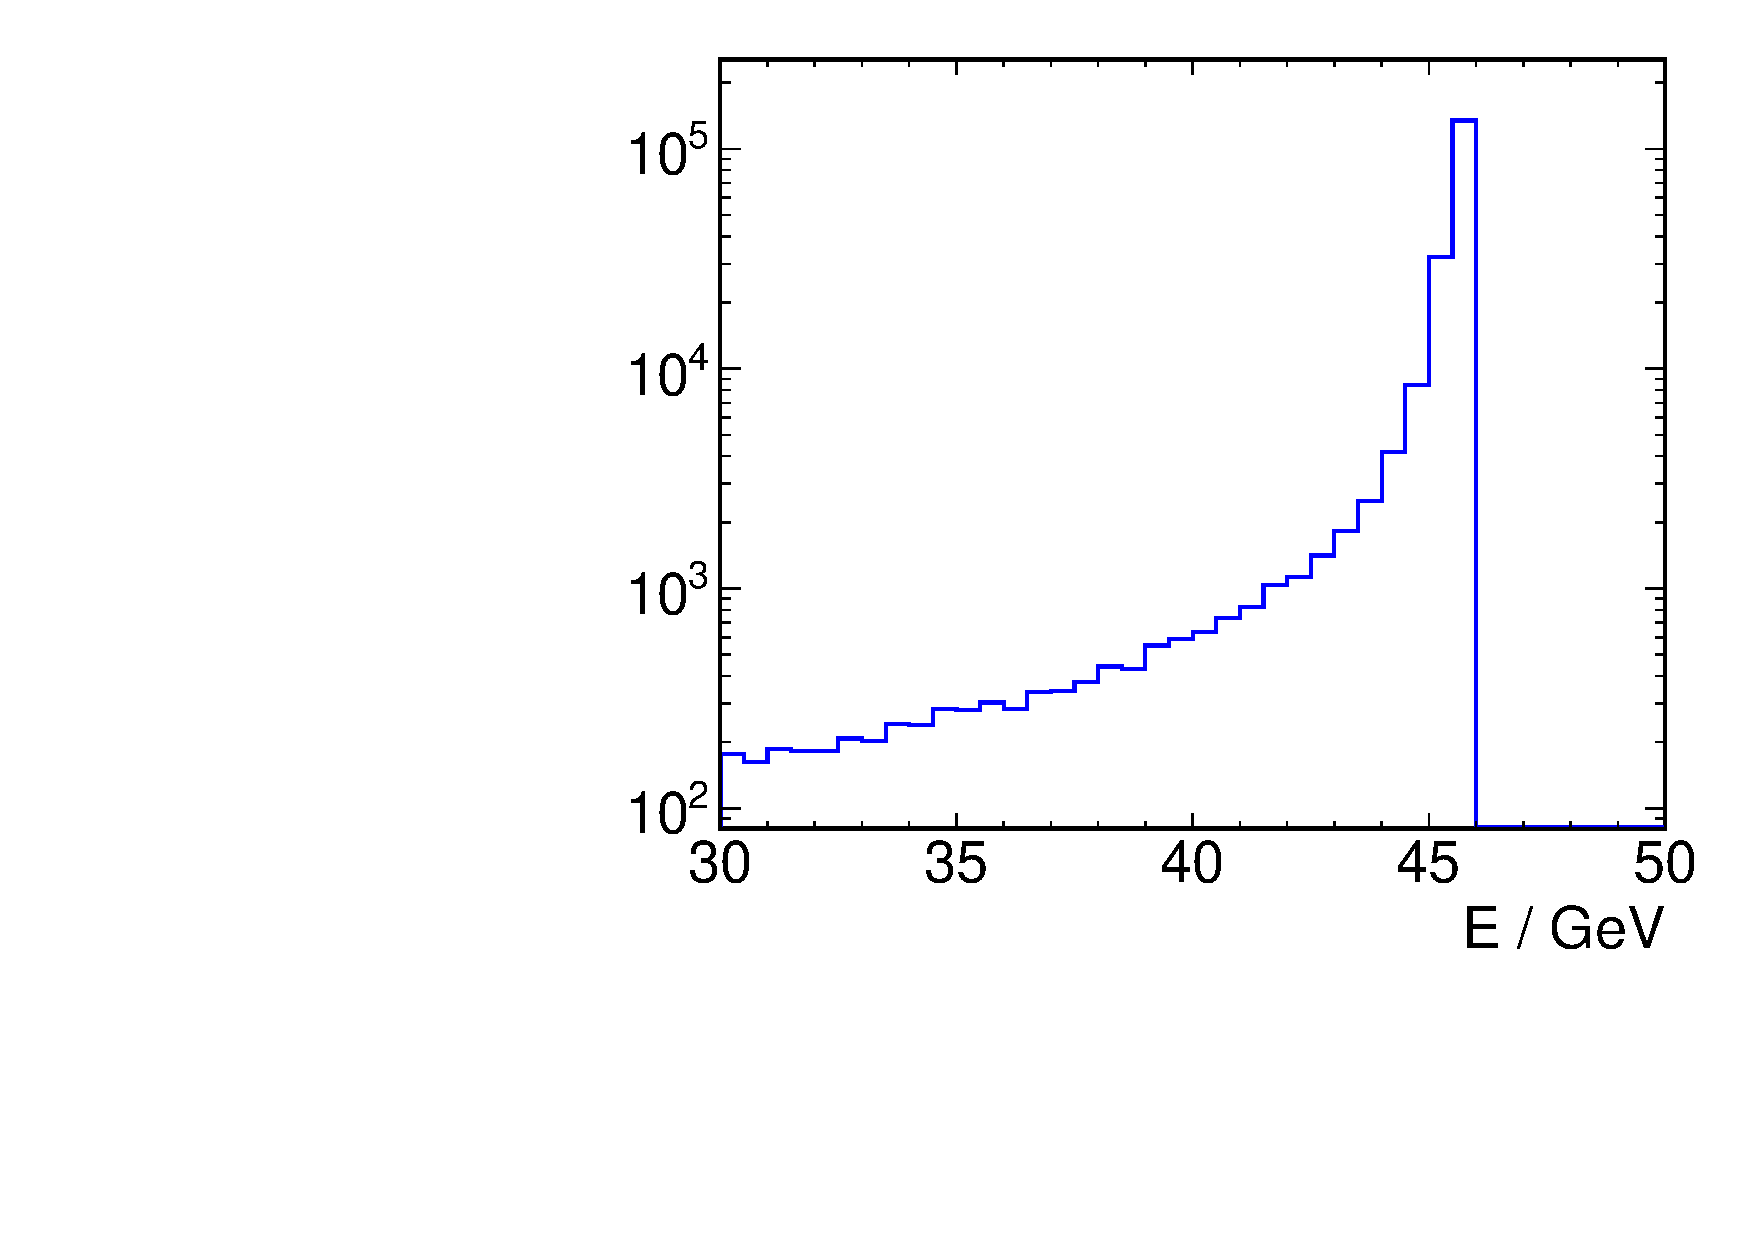
\includegraphics[width=\linewidth]{Fig8_mumu_E.pdf}
  \caption{}
\end{subfigure}
\caption{Generator-level distributions of (a)~$\cos\theta$, (b)~$\phi$,
and (c)~energy of muons in $e^{+}e^{-}\to\mu^{+}\mu^{-}$ at
$\sqrt{s}=\SI{91.2}{GeV}$.}
\label{fig:kinematic_mumu}
\end{figure}

\begin{figure}[htbp]
\centering
\includegraphics[width=0.50\textwidth]{Mjj_eeuu_91.pdf}
\caption{Distribution of dijet invariant mass from $Z\to q\bar{q}$ at
$\sqrt{s}=\SI{91.2}{GeV}$.}
\label{fig:kinematic_zjj}
\end{figure}

\paragraph{Hardware calibration.}
The hardware calibration comprises MIP inter-calibration using cosmic
rays or muon beams, and an online LED-based monitoring system with
optical-fibre distribution to multiple cells
(Figure~\ref{fig:Calibration-2n}).
The LED system continuously tracks pedestals, gain, and response
linearity at the single-cell level.

\begin{figure}[htbp]
\centering
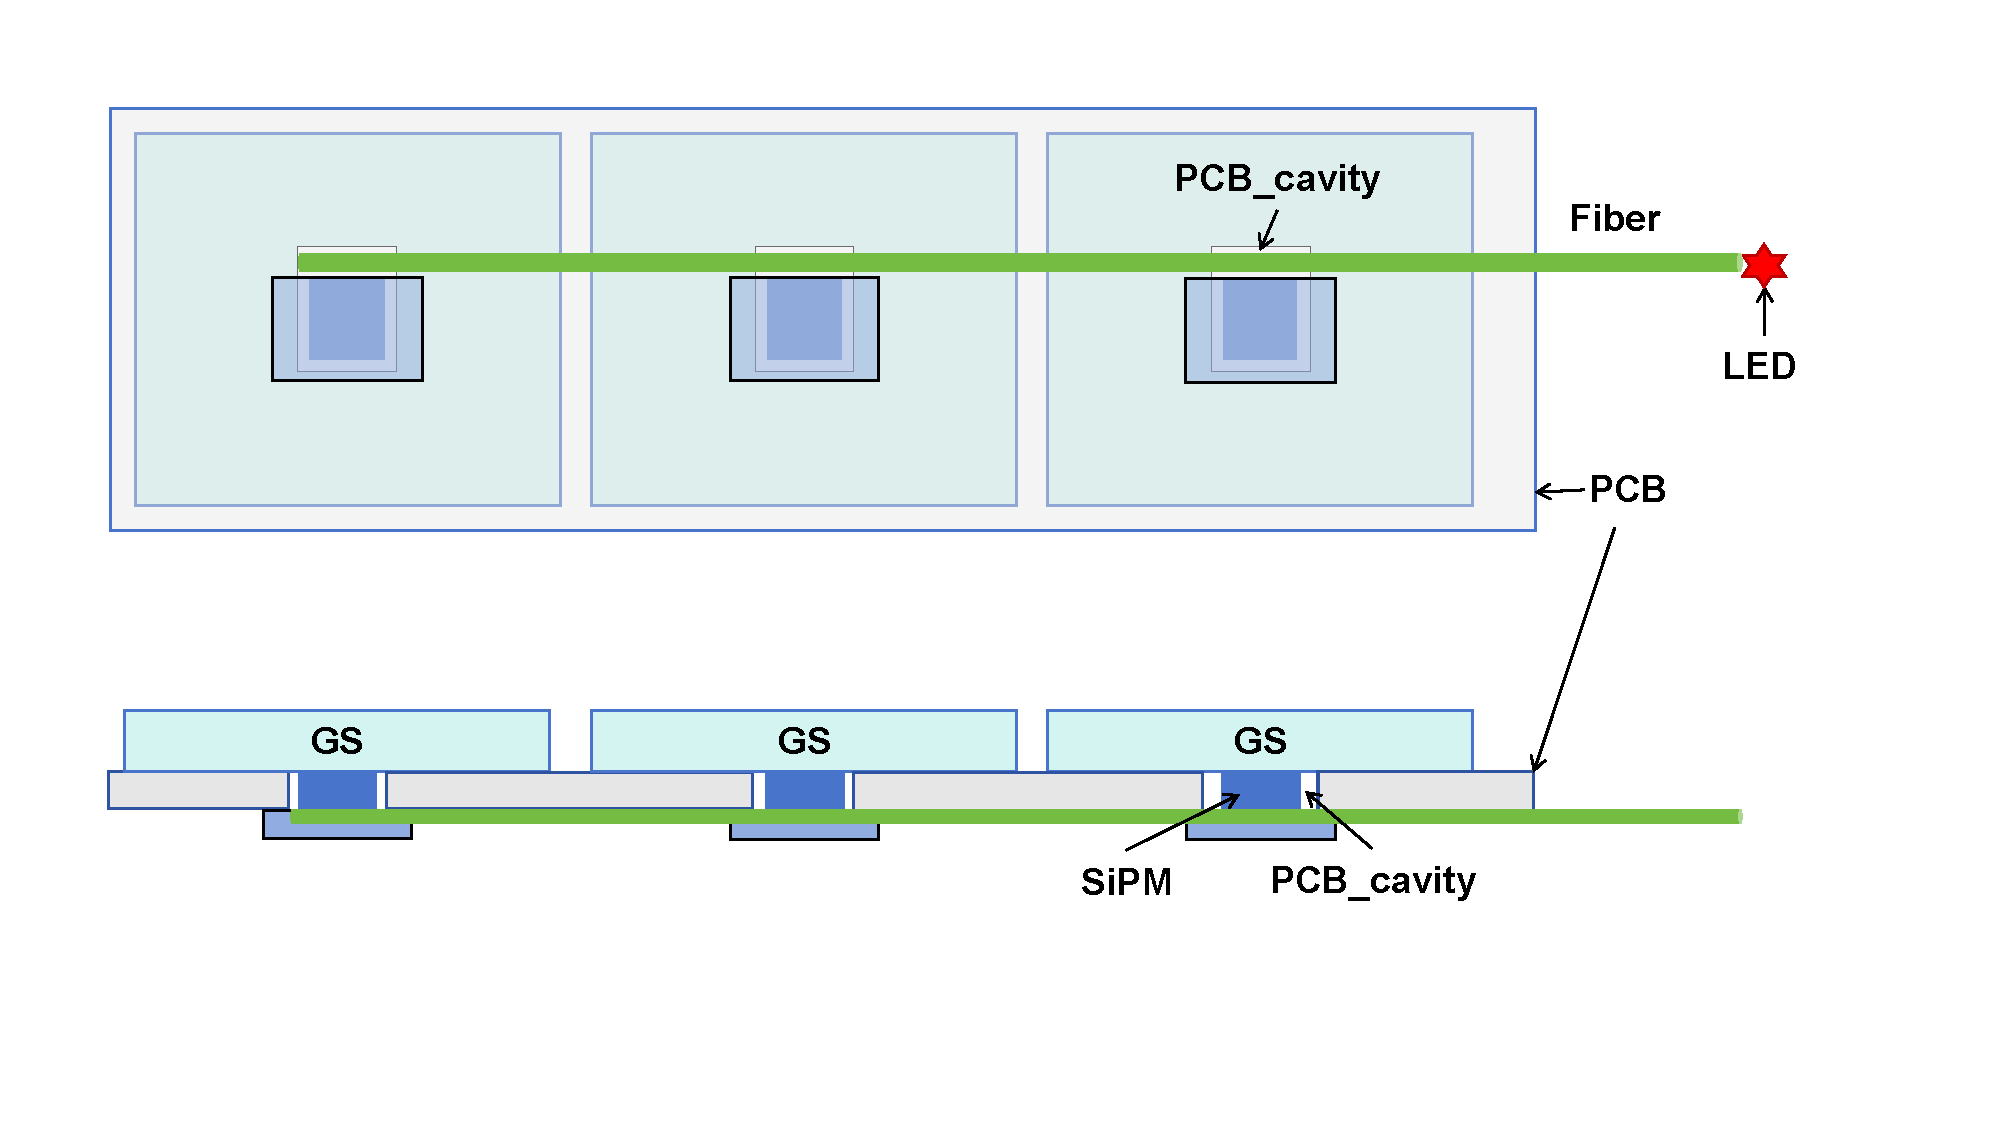
\includegraphics[width=0.68\textwidth]{Calibration-2n.pdf}
\caption{Schematic of the GS-HCAL LED calibration system showing
optical-fibre connections between adjacent cells: top~view~(a) and
side~view~(b).}
\label{fig:Calibration-2n}
\end{figure}

The two layers are complementary: the physics-process layer provides
absolute energy-scale closure in situ, while the hardware layer
provides the fast monitoring loop between physics calibrations.
The baseline design cannot be realised without both, and this is why
they are presented as components of the detector concept rather than
as post-hoc add-ons.

%% --------------------------------------------------------------------
\subsection{Prototype validation strategy}
\label{subsec:prototype}
%% --------------------------------------------------------------------

A GS-HCAL prototype is under construction to provide the validation
path of the baseline detector concept.
The prototype is a steel-scintillator sandwich of
$52.0\times52.0\times130.6$~cm$^{3}$ (${\approx}0.6$~m$^{3}$),
containing 8112~GS cells in 48~layers (${\approx}6\,\lambdaI$).
Each layer is a $13\times13$ array of \cellsize cells, each coupled
to a \sipmsize SiPM, with \SI{9.8}{mm} S304 stainless-steel absorber
plates.

Geant4 simulations with \SI{80}{GeV} $\pi^{-}$ beams show that this
$13\times13\times48$ configuration reaches 95\% energy containment
(Figure~\ref{fig:prototype-sim-energy}), and projects a prototype
single-hadron resolution of ${\sim}45\%/\sqrt{E}\oplus8\%$,
degraded relative to the full detector because of the limited
transverse extent but sufficient to validate the key baseline
technologies and reconstruction algorithms
(Figure~\ref{fig:prototype-sim-resolution}).

\begin{figure}[htbp]
\centering
\includegraphics[width=0.50\linewidth]{Edep_module_80GeV.pdf}
\caption{Simulated deposited energy in prototypes of different lateral
sizes for \SI{80}{GeV} $\pi^{-}$; the $13\times13\times48$
configuration achieves ${\approx}95\%$ containment.}
\label{fig:prototype-sim-energy}
\end{figure}

\begin{figure}[htbp]
\centering
\begin{subfigure}{0.40\textwidth}
  \centering
  \includegraphics[width=\linewidth]{prototype_simulation-13}
  \caption{}
\end{subfigure}\hfill
\begin{subfigure}{0.40\textwidth}
  \centering
  \includegraphics[width=\linewidth]{prototype_simulation-linear.jpg}
  \caption{}
\end{subfigure}
\caption{Simulated (a)~energy resolution and (b)~energy linearity of
the GS-HCAL prototype.}
\label{fig:prototype-sim-resolution}
\end{figure}

The validation proceeds in two stages:
a $3\times3\times7$ mini-prototype tests integration of the GS cell,
SiPM, front-end, and calibration at reduced scale;
the full 8112-channel prototype then exercises the complete baseline
active unit and provides the measured detector response against which
the Geant4 optical model, the Birks constant, the intrinsic $e/h$
extraction, and the constant-term interpretation can be closed.
Together with the measured containment and projected prototype
resolution, this establishes a clear closure path from the
current evidence to a fully validated baseline.

%% ====================================================================
\section{Discussion}
\label{sec:discussion}
%% ====================================================================

The foregoing sections have established the design logic, material
characterisation, simulation performance, and engineering feasibility
of the GS-HCAL baseline.
It is now useful to assess coherently what has been established, what
remains uncertain, and what the immediate validation priorities are.

%% --------------------------------------------------------------------
\subsection{What has been established}
\label{subsec:established}
%% --------------------------------------------------------------------

The baseline architecture is defined as a barrel+endcap,
$6\,\lambdaI$ deep, 48~layers of \cellsize GFO cells read out by
\sipmsize SiPMs, with approximately 5.22~million channels.
The active medium has been identified as GFO glass, with measured
intrinsic light yield $>\SI{1000}{\phMeV}$, attenuation length
${\sim}\SI{6}{cm}$, and radiation tolerance retaining more than 70\%
of the initial light yield at \SI{100}{Gy}.
Cell-level readout feasibility is demonstrated by single-cell
measurements with $^{137}$Cs, cosmic-ray muons
(${63.6\pm0.5}$~\peMIP), and \SI{5}{GeV} electrons at KEK
(${157.6\pm2.9}$~\peMIP), and by the interim pre-amplifier
performance.
SiPM compatibility with the baseline cell is demonstrated by the DCR
versus threshold behaviour at the \SI{0.1}{MIP} working point.
Full digitisation-based system simulation predicts a single-hadron
energy resolution of $29.8\%/\sqrt{E}\oplus6.5\%$ and an $H\to gg$
BMR of 3.88\%, consistent with the CEPC target of 3--4\%.
Mechanical finite-element analysis demonstrates feasibility at
detector scale.
A two-layer calibration architecture has been defined as an integral
part of the baseline.

%% --------------------------------------------------------------------
\subsection{What remains uncertain}
\label{subsec:uncertain}
%% --------------------------------------------------------------------

The following items have \emph{not} yet been experimentally closed
and collectively define the open boundary of the baseline:

\begin{itemize}
\item \textbf{Full-prototype beam validation} is not yet complete; the
  8112-channel prototype is under construction and its beam-test
  closure is the principal missing experimental step.
\item \textbf{Geant4 optical parameters} for GFO require tuning: the
  simulated single-cell light yield (${\sim}42$~\peMIP) is below the
  measured cosmic-ray value (${\sim}64$~\peMIP).
\item \textbf{Birks' constant} used in the digitisation model is
  preliminary; a dedicated heavy-ion measurement is planned.
\item \textbf{Intrinsic $e/h$} has not yet been extracted through
  shower-component decomposition; only the empirical
  $C_{\mathrm{hadron}}/C_{e}$ is currently available.
\item \textbf{Constant term} of ${\approx}5$--6\% is linked to
  longitudinal leakage; its expected reduction with full-detector
  environment and software compensation is demonstrated only in
  simulation.
\item \textbf{Tile production yield and uniformity} still require
  optimisation: only about 60\% of produced tiles currently meet the
  \SI{1000}{\phMeV} target.
\end{itemize}

%% --------------------------------------------------------------------
\subsection{Why these uncertainties do not invalidate the baseline
choice}
\label{subsec:rationale-uncertainty}
%% --------------------------------------------------------------------

A baseline choice in a detector concept does not require that every
uncertainty be closed simultaneously and in advance.
What it requires is that the combined evidence identifies a single
integrated technology direction that is already supported at the
material, cell, system, and engineering levels, and that the
remaining uncertainties are well localised, fully characterised,
and attached to an explicit closure path.
The present GS-HCAL results satisfy this criterion: the baseline
architecture, the active medium, the readout, the simulation
framework, and the calibration and mechanical strategies all stand on
measured or simulation-based evidence, while the open items of
Section~\ref{subsec:uncertain} are individually attached to the
prototype programme of Section~\ref{subsec:prototype} and to the
immediate priorities below.

%% --------------------------------------------------------------------
\subsection{Immediate priorities}
\label{subsec:priorities}
%% --------------------------------------------------------------------

The immediate priorities are:
\begin{itemize}
\item prototype beam tests, to provide the first measured closure of
  the detector-level response;
\item Geant4 optical-model tuning against measured GFO data, to
  close the simulation--measurement discrepancy on the single-cell
  light yield;
\item intrinsic $e/h$ extraction and implementation of software
  compensation, to bring the constant term towards the final target;
\item development of the low-power ASIC and its system-level
  integration.
\end{itemize}

%% ====================================================================
\section{Conclusion}
\label{sec:conclusion}
%% ====================================================================

The Glass-Scintillator HCAL is adopted as the baseline HCAL of the
CEPC reference detector, and the present study establishes the design
logic and technical basis of that choice.

The baseline evidence combines measured GFO material performance,
single-cell readout demonstrated with three independent probes, SiPM
operation at a working threshold compatible with the measured dark
count rate, full-detector Geant4 digitisation predicting a
single-hadron resolution of $29.8\%/\sqrt{E}\oplus6.5\%$ and an
$H\to gg$ BMR of 3.88\%, detector-scale mechanical feasibility, and a
calibration architecture integrated into the detector concept from
the outset.
These measured, simulated, and engineering lines of evidence are
coherent and together support the baseline.

Full prototype beam tests remain essential for the final experimental
validation of the baseline detector concept; they are the next step
in closing the items listed in Section~\ref{subsec:uncertain}, and
they define the validation path from the present technical basis to a
fully validated baseline HCAL.

%% ====================================================================
\section*{Acknowledgements}
%% ====================================================================

The authors thank all members of the CEPC Study Group for their
contributions to the physics and detector design studies.
We are grateful to the CALICE Collaboration for extensive test-beam
data and collaborative R\&D efforts, and to the staff of the KEK
test-beam facility and the APEP proton-irradiation facility for
experimental support.
This work is supported in part by
the National Key Research and Development Program of China
(Grant No.~2020YFA0406200),
the Chinese Academy of Sciences (Grant No.~XDB34000000),
the National Natural Science Foundation of China (NSFC,
Grant Nos.~12075265 and~12105295),
and the CEPC detector R\&D programme.

%% ====================================================================
%% References
%% ====================================================================
%% The bibliography style is set by each wrapper via \bibliostyle
%% before %% ====================================================================
%% GS-HCAL paper — shared body text
%% Baseline detector-technology paper for the CEPC reference detector
%% ====================================================================

%% ====================================================================
\section{Introduction}
\label{sec:intro}
%% ====================================================================

The Circular Electron-Positron Collider
(CEPC)~\cite{CEPCStudyGroup:2018ghi} will operate as a Higgs factory at
$\sqrt{s}=240$~GeV and as a high-luminosity $Z$-pole machine at
$\sqrt{s}=91.2$~GeV.
Within the Particle-Flow Algorithm
(PFA)~\cite{Thomson:2009rp,Brient:2004yq,Ruan:2013rkk} paradigm, the
Hadronic Calorimeter (HCAL) is responsible for the precise spatial
reconstruction and energy measurement of neutral hadrons, which carry
approximately 10\% of the jet energy and leave no tracks in the central
tracker.
The target boson mass resolution (BMR) of
3--4\%~\cite{CEPCStudyGroup:2018ghi} for $W$/$Z$/Higgs dijet final
states directly depends on the HCAL performance.
These requirements are satisfied only when the HCAL simultaneously
provides fine three-dimensional granularity, sufficient depth, and
adequate energy resolution.

The baseline choice is driven not by a single metric, but by the
combined requirements of neutral-hadron measurement, high granularity
for particle flow, compactness, active-material density, scalable cell
production, SiPM-compatible readout, and detector-scale integration.
The Glass-Scintillator HCAL
(GS-HCAL)~\cite{Tang:2022yrb,Hu:2023dbm,Hu:2024nvo} is adopted as the
baseline HCAL of the CEPC reference detector because it is the only
mature integrated technology that satisfies all of these requirements
simultaneously, while being supported by measured material performance,
validated single-cell readout, full-detector digitisation simulation,
and an established mechanical and calibration concept.
Alternative HCAL technologies exist, but they are outside the scope of
this paper.

The remainder of this paper reports:
the physics- and technology-driven design requirements and the
rationale for the baseline choice (Section~\ref{sec:rationale});
the detector-scale architecture and system design
(Section~\ref{sec:design});
the active-unit implementation, comprising the GFO glass, the SiPM
readout, the front-end electronics, and the supporting optical
simulation (Section~\ref{sec:activeunit});
the experimental characterisation of the baseline active unit
(Section~\ref{sec:expchar});
the simulation framework and projected detector performance
(Section~\ref{sec:simperf});
the mechanical feasibility, calibration strategy, and prototype
validation path (Section~\ref{sec:feasibility});
a discussion of established results and remaining uncertainties
(Section~\ref{sec:discussion});
and a concluding summary (Section~\ref{sec:conclusion}).

\begin{figure}[htbp]
\centering
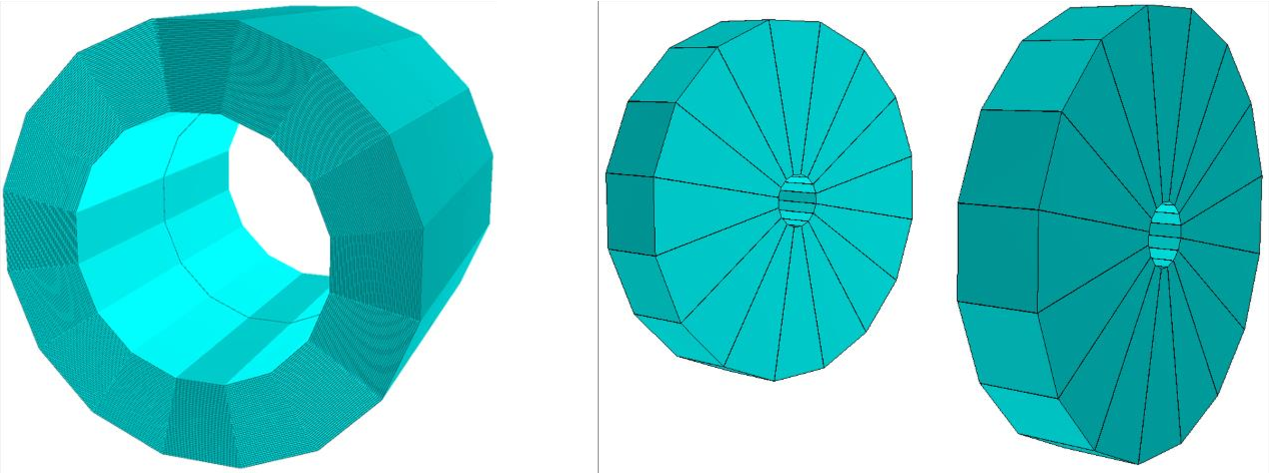
\includegraphics[width=0.9\textwidth]{Geometry.pdf}
\caption{Geometric configuration of the GS-HCAL system.
Left: barrel with 16~trapezoidal sectors forming a cylindrical structure
(inner diameter \SI{4280}{mm}, outer diameter \SI{6910}{mm}).
Right: endcap disks with matching sector segmentation.}
\label{fig:GS-geometry}
\end{figure}

%% ====================================================================
\section{Design requirements and baseline rationale}
\label{sec:rationale}
%% ====================================================================

The adoption of the GS-HCAL as the baseline HCAL of the CEPC
reference detector rests on the convergence of three independent lines
of argument: the physics requirements imposed by the CEPC programme
and the PFA paradigm; the technology requirements that any candidate
HCAL must simultaneously satisfy; and the specific combination of
measured and simulated properties that makes GS-HCAL the most mature
integrated technology satisfying all of them together.

%% --------------------------------------------------------------------
\subsection{Physics-driven requirements}
\label{subsec:physics-req}
%% --------------------------------------------------------------------

In the PFA paradigm the HCAL must independently measure neutral
hadrons---primarily neutrons and $K_{L}^{0}$ mesons---that leave no
tracks in the central tracker and carry approximately 10\% of the jet
energy.
These particles are the dominant source of resolution degradation in
PFA jet reconstruction, because their energy must be taken directly
from the calorimeter rather than from the tracker.
The CEPC target BMR of 3--4\% for $W/Z$/Higgs dijet final states
therefore translates into stringent HCAL requirements:
\begin{itemize}
\item Fine three-dimensional granularity is required to separate
  neutral-hadron clusters from nearby charged-particle energy deposits
  and to enable longitudinal shower analysis.
\item Sufficient depth, typically $\gtrsim6\,\lambdaI$ in the
  HCAL~itself, is required to contain hadronic showers and minimise
  longitudinal leakage.
\item The energy response must be close to linear and well-calibrated
  across the relevant range (${\sim}0.5$--\SI{60}{GeV}) so that PFA
  reconstruction of jet substructure remains robust.
\item Good single-hadron resolution also benefits searches for
  long-lived particles that may decay within the HCAL volume.
\end{itemize}

%% --------------------------------------------------------------------
\subsection{Technology-driven requirements}
\label{subsec:tech-req}
%% --------------------------------------------------------------------

Any HCAL technology candidate for the CEPC reference detector must
simultaneously satisfy the following integrated requirements:

\begin{itemize}
\item \textbf{Active-medium density:} higher density reduces the
  detector envelope for a fixed number of nuclear interaction lengths,
  which is critical in the limited radial budget of the reference
  detector.
\item \textbf{Cell granularity at the $40\times40$~mm$^{2}$ scale:}
  required for PFA shower separation; must be reproducibly
  manufacturable at that scale.
\item \textbf{SiPM-compatible light output:} the active medium must
  produce enough scintillation light that a compact SiPM readout can
  operate at a \SI{0.1}{MIP} threshold while suppressing dark-count
  noise.
\item \textbf{Scalability to approximately 5.22~million channels:} the
  production, assembly, and quality-control procedures must be
  compatible with the resulting system-level complexity.
\item \textbf{Radiation tolerance:} optical performance must be
  retained under the accumulated doses expected during Higgs and
  $Z$-pole operation.
\item \textbf{Thermal and electronics integration:} the front-end
  electronics, cooling, and mechanical support must be accommodated
  within the available layer thickness.
\item \textbf{Modular assembly feasibility:} the detector must be
  buildable, installable, and serviceable at realistic engineering
  tolerances.
\end{itemize}

These requirements must be satisfied \emph{together}---a technology
that excels in only a subset of them is not a viable baseline.

%% --------------------------------------------------------------------
\subsection{Why GS-HCAL is adopted as the baseline}
\label{subsec:why-baseline}
%% --------------------------------------------------------------------

The GS-HCAL is adopted as the baseline because the combined evidence
from materials R\&D, single-cell measurements, full-detector
digitisation simulation, and engineering analysis shows that it is the
most mature technology that satisfies the requirements of
Sections~\ref{subsec:physics-req} and~\ref{subsec:tech-req}
simultaneously.
The supporting evidence is of three distinct types, which are kept
separate throughout this paper:
(A)~experimentally measured properties of GFO cells and SiPM readout;
(B)~full-detector Geant4 digitisation simulation of the baseline
geometry; and (C)~analyses whose final closure depends on ongoing
prototype beam tests.

Specifically, the baseline choice is supported by the following five
points.

\begin{enumerate}
\item \textbf{Active-medium density (A).}
  GFO glass provides a density of \SI{6.0}{g/cm^{3}}, substantially
  higher than plastic scintillator (${\sim}\SI{1.03}{g/cm^{3}}$),
  while remaining manufacturable at the $40\times40\times10$~mm$^{3}$
  cell scale and delivering a measured intrinsic light yield
  $>\SI{1000}{\phMeV}$ (Sections~\ref{subsec:gfo}
  and~\ref{subsec:lightyield}).
\item \textbf{Cell geometry and PFA compatibility (A+B).}
  The \cellsize cell geometry, combined with \sipmsize SiPM readout,
  is compatible with highly granular PFA calorimetry; measured
  single-cell light outputs of 60--100~\peMIP
  (Section~\ref{subsec:cellmeas}) establish that practical SiPM
  operation is achievable at the required threshold.
\item \textbf{Radiation tolerance (A).}
  The GFO light yield retains more than 70\% of its initial value at
  \SI{100}{Gy} (Section~\ref{subsec:radiation}), which covers the
  accumulated dose expected over the CEPC operational scenarios.
\item \textbf{Projected detector performance (B).}
  Full digitisation-based Geant4 simulation of the baseline geometry
  predicts a single-hadron energy resolution of
  $\sigma_{E}/E = 29.8\%/\sqrt{E}\oplus6.5\%$ and an $H\to gg$ BMR of
  3.88\%, consistent with the CEPC target of 3--4\%
  (Sections~\ref{subsec:hadronres} and~\ref{subsec:physperf}).
\item \textbf{Detector-scale feasibility (A+B).}
  Finite-element analysis of the modular-box architecture demonstrates
  mechanical feasibility under the full load including the ECAL, and
  the water-cooling and calibration concepts are compatible with the
  channel count and dissipation
  (Sections~\ref{subsec:architecture}--\ref{subsec:channels}
  and~\ref{subsec:mechanics}).
\end{enumerate}

Categories~A and~B together establish the technical basis of the
baseline.
Final experimental closure, category~C, requires prototype beam tests
and is the subject of Section~\ref{subsec:prototype}.

%% --------------------------------------------------------------------
\subsection{Boundaries and remaining work}
\label{subsec:boundaries}
%% --------------------------------------------------------------------

The baseline rationale is transparent about what has \emph{not} yet
been experimentally closed.
Before proceeding to the detailed design and characterisation, the
principal boundaries of the current evidence are summarised here:

\begin{itemize}
\item Full prototype beam validation has not yet been performed; the
  8112-channel prototype is under construction
  (Section~\ref{subsec:prototype}).
\item The Geant4 optical model of GFO requires further tuning: the
  simulated single-cell light yield (${\sim}42$~\peMIP) is lower
  than the cosmic-ray measurement (${\sim}64$~\peMIP)
  (Section~\ref{subsec:optsim}).
\item The Birks constant used in the digitisation model is
  preliminary; a dedicated heavy-ion measurement is planned
  (Section~\ref{subsec:simsetup}).
\item The intrinsic $e/h$ compensation ratio has not yet been
  extracted from shower-component decomposition
  (Section~\ref{subsec:eresponse}).
\item The constant term (${\approx}5$--6\%) is currently dominated by
  longitudinal leakage in the $6\,\lambdaI$ design
  (Section~\ref{subsec:constterm}).
\item Tile production yield and light-yield uniformity still require
  optimisation: at present only about 60\% of produced tiles exceed
  the \SI{1000}{\phMeV} target (Section~\ref{subsec:qc}).
\end{itemize}

These items are discussed systematically in
Section~\ref{sec:discussion}.
They define the validation path of the baseline, but they do not
invalidate the baseline choice itself: a baseline identifies the most
mature and best-supported integrated technology direction, not a
concept whose every uncertainty is already experimentally closed.

%% ====================================================================
\section{Baseline detector concept and system design}
\label{sec:design}
%% ====================================================================

The baseline concept is realised at detector scale through a
barrel-plus-endcap architecture with 48~longitudinal layers of
\cellsize GFO cells.
Each design choice is driven by one or more of the requirements
established in Section~\ref{sec:rationale}, and the motivation is
given before the corresponding parameters.

%% --------------------------------------------------------------------
\subsection{Overall architecture}
\label{subsec:architecture}
%% --------------------------------------------------------------------

The overall architecture is driven by three requirements:
hermetic geometric coverage for PFA, sufficient depth for hadronic
containment, and a granularity compatible with shower separation in
the CEPC jet environment.
These requirements are met by a barrel with two endcaps, each
segmented into 16~trapezoidal sectors of 48~longitudinal layers and a
total depth of $6\,\lambdaI$ in steel and GS
(Figure~\ref{fig:GS-geometry}).
The barrel has inner and outer radii of \SI{2140}{mm} and
\SI{3455}{mm} and a length of \SI{6460}{mm} along the beam axis; the
endcaps match this segmentation with inner and outer radii of
\SI{450}{mm} and \SI{3455}{mm}.
The complete detector contains approximately 5.22~million identical
\cellsize GFO cells, each read out by a \sipmsize SiPM; the
corresponding sampling fraction is approximately 31\%.

%% --------------------------------------------------------------------
\subsection{Single-layer design as the fundamental baseline unit}
\label{subsec:onelayer}
%% --------------------------------------------------------------------

The single-layer design is the fundamental unit of the baseline
detector concept.
It is chosen so that the active GS layer, the SiPM plus PCB readout,
the ASIC cooling, and the steel absorber all fit within a compact
layer thickness while preserving the sampling fraction and mechanical
tolerances required by the PFA design.
Each layer has a total thickness of \SI{27.2}{mm}, corresponding to
approximately $0.125\,\lambdaI$, and contains from top to bottom:
a \SI{2}{mm} upper cover plate;
the \SI{10}{mm} GS active layer of $40\times40$~mm$^{2}$ cells;
a \SI{3.2}{mm} PCB layer carrying the front-end ASICs;
a \SI{2}{mm} bottom cover; and
a \SI{9.8}{mm} steel absorber in which cooling pipes of \SI{3}{mm}
outer radius are embedded.
One SiPM is positioned at the centre of each GS cell on a PCB shared
by multiple cells.
The nuclear-interaction-length contributions of the steel absorber,
the GS active layer, and the PCB are in the ratio $1:0.53:0.03$,
giving a sampling fraction of approximately 31\%.

\begin{figure}[htbp]
\centering
\begin{subfigure}{0.50\linewidth}
  \centering
  \includegraphics[width=\linewidth]{GS-HCAL-cell.pdf}
  \caption{}
  \label{fig:gshcal-cell-a}
\end{subfigure}%
\begin{subfigure}{0.35\linewidth}
  \centering
  \includegraphics[width=\linewidth]{GSHCALOneCell1.pdf}
  \caption{}
  \label{fig:gshcal-cell-b}
\end{subfigure}
\caption{(a)~Single-layer structure of the GS-HCAL\@.
(b)~One GS cell of \cellsize.}
\label{fig:gshcal-cell}
\end{figure}

%% --------------------------------------------------------------------
\subsection{Barrel implementation}
\label{subsec:barrel}
%% --------------------------------------------------------------------

The barrel is divided into 16~trapezoidal sectors
(Figure~\ref{fig:BarrelContourDimension}), each having a front width
of \SI{851}{mm}, a back width of \SI{1375}{mm}, and a radial thickness
of \SI{1315}{mm} ($6\,\lambdaI$).
The longitudinal segmentation into 48~layers follows the PFA
optimisation performed with the Plastic-Scintillator HCAL
prototype~\cite{CALICE:2010fpb}.
The total barrel weight is \SI{955}{t}
(Table~\ref{tab:BarrelWeight}).

Each layer consists of a continuous steel absorber plate over the full
barrel length, onto which modular detection boxes are mounted.
Each box contains a complete detection unit---GS cells, SiPMs, PCB,
ASICs, cables, and cover plates---with three standard box widths
(\SI{320}{mm}, \SI{280}{mm}, \SI{240}{mm}) combined to follow the
trapezoidal geometry while preserving the uniform \cellsize~cell
granularity (Figure~\ref{fig:BarrelModuleStructure}).
The 16~radial sector boundaries introduce projective cracks, but these
are effectively compensated by the upstream BGO ECAL
(${\approx}1.2\,\lambdaI$), which initiates most hadronic showers
before the HCAL and produces lateral spread bridging the sector
boundaries.

\begin{figure}[htbp]
\centering
\begin{subfigure}{0.42\linewidth}
  \centering
  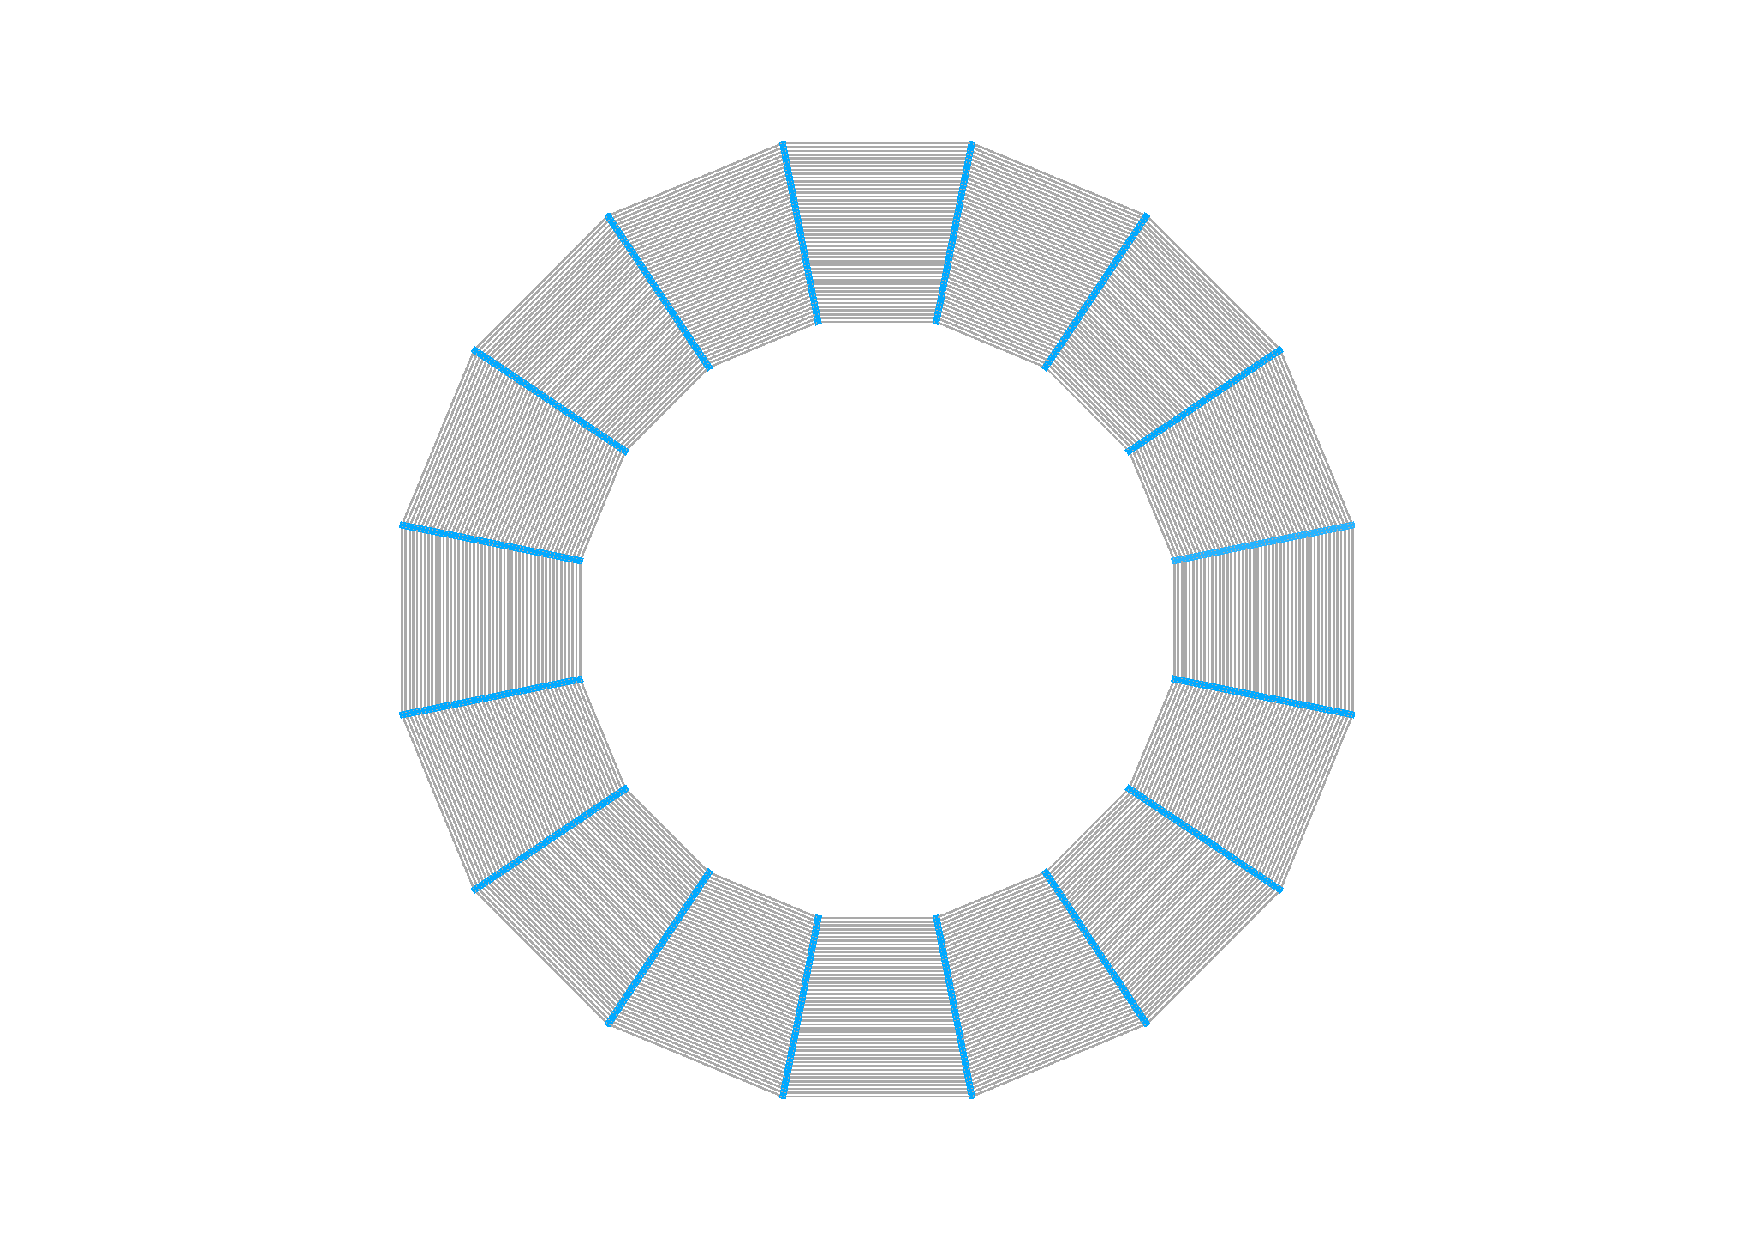
\includegraphics[width=\linewidth,trim=160pt 50pt 160pt 50pt,clip]{BarrelView1.pdf}
  \caption{}
\end{subfigure}\hfill
\begin{subfigure}{0.45\linewidth}
  \centering
  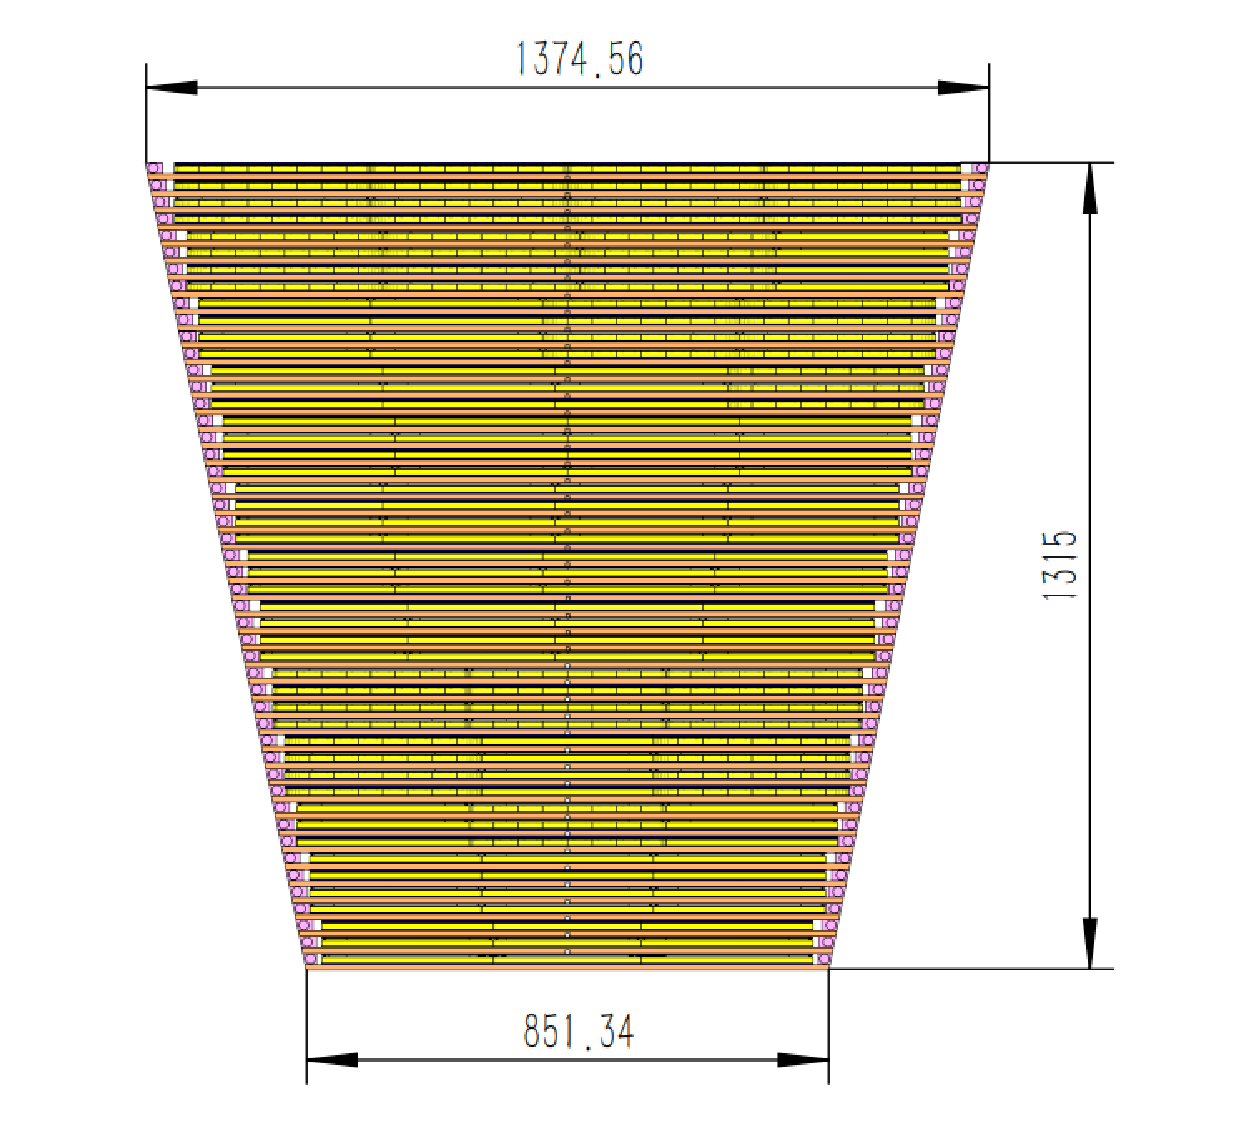
\includegraphics[width=\linewidth]{HCALBarrelOneSector.pdf}
  \caption{}
\end{subfigure}
\caption{Dimensions of the GS-HCAL barrel.
(a)~Cross-sectional view showing 16~trapezoidal sectors
(inner diameter \SI{4280}{mm}, outer diameter \SI{6910}{mm}).
(b)~Side view of a single trapezoidal sector.}
\label{fig:BarrelContourDimension}
\end{figure}

\begin{figure}[htbp]
\centering
\includegraphics[width=0.9\linewidth]{Fig.1.81-Boxes_dimension-and_more-structure_details.pdf}
\caption{GS-HCAL barrel sector structure.
(a)~Full sector composed of 48~layers.
(b)~Dimensions of an individual box.
(c)~Internal structure of a box with cover plates, GS cells, PCB
with ASICs, cables, and cooling-water pipes.}
\label{fig:BarrelModuleStructure}
\end{figure}

\begin{table}[htbp]
\centering
\caption{Weight breakdown of the barrel GS-HCAL\@.}
\label{tab:BarrelWeight}
\begin{tabular}{l S[table-format=5.0] S[table-format=3.1]}
\toprule
\textbf{Component} & {\textbf{Weight/sector (kg)}} & {\textbf{Weight/barrel (t)}} \\
\midrule
Cover plate        & 10287 & 164.6 \\
PCB plate          &   390 &   6.2 \\
Glass scintillator & 19277 & 308.4 \\
Absorber layer     & 27515 & 440.2 \\
Support structure  &  1883 &  30.1 \\
Auxiliaries        &   350 &   5.6 \\
\midrule
Total              & 59702 & 955.2 \\
\bottomrule
\end{tabular}
\end{table}

%% --------------------------------------------------------------------
\subsection{Endcap implementation}
\label{subsec:endcap}
%% --------------------------------------------------------------------

The two endcaps complete the geometric coverage along the beam
direction (Figure~\ref{fig:EndcapsOverall}).
Each endcap mirrors the barrel segmentation with 16~disk-shaped
sectors, inner and outer radii of \SI{450}{mm} and \SI{3455}{mm}, and a
total thickness of \SI{1315}{mm} in 48~layers.
A single sector has a top width of \SI{1307}{mm} and a radial height of
\SI{2862}{mm}, and is divided radially into six boxes.
Each endcap weighs \SI{362}{t}.

\begin{figure}[htbp]
\centering
\begin{subfigure}{0.58\linewidth}
  \centering
  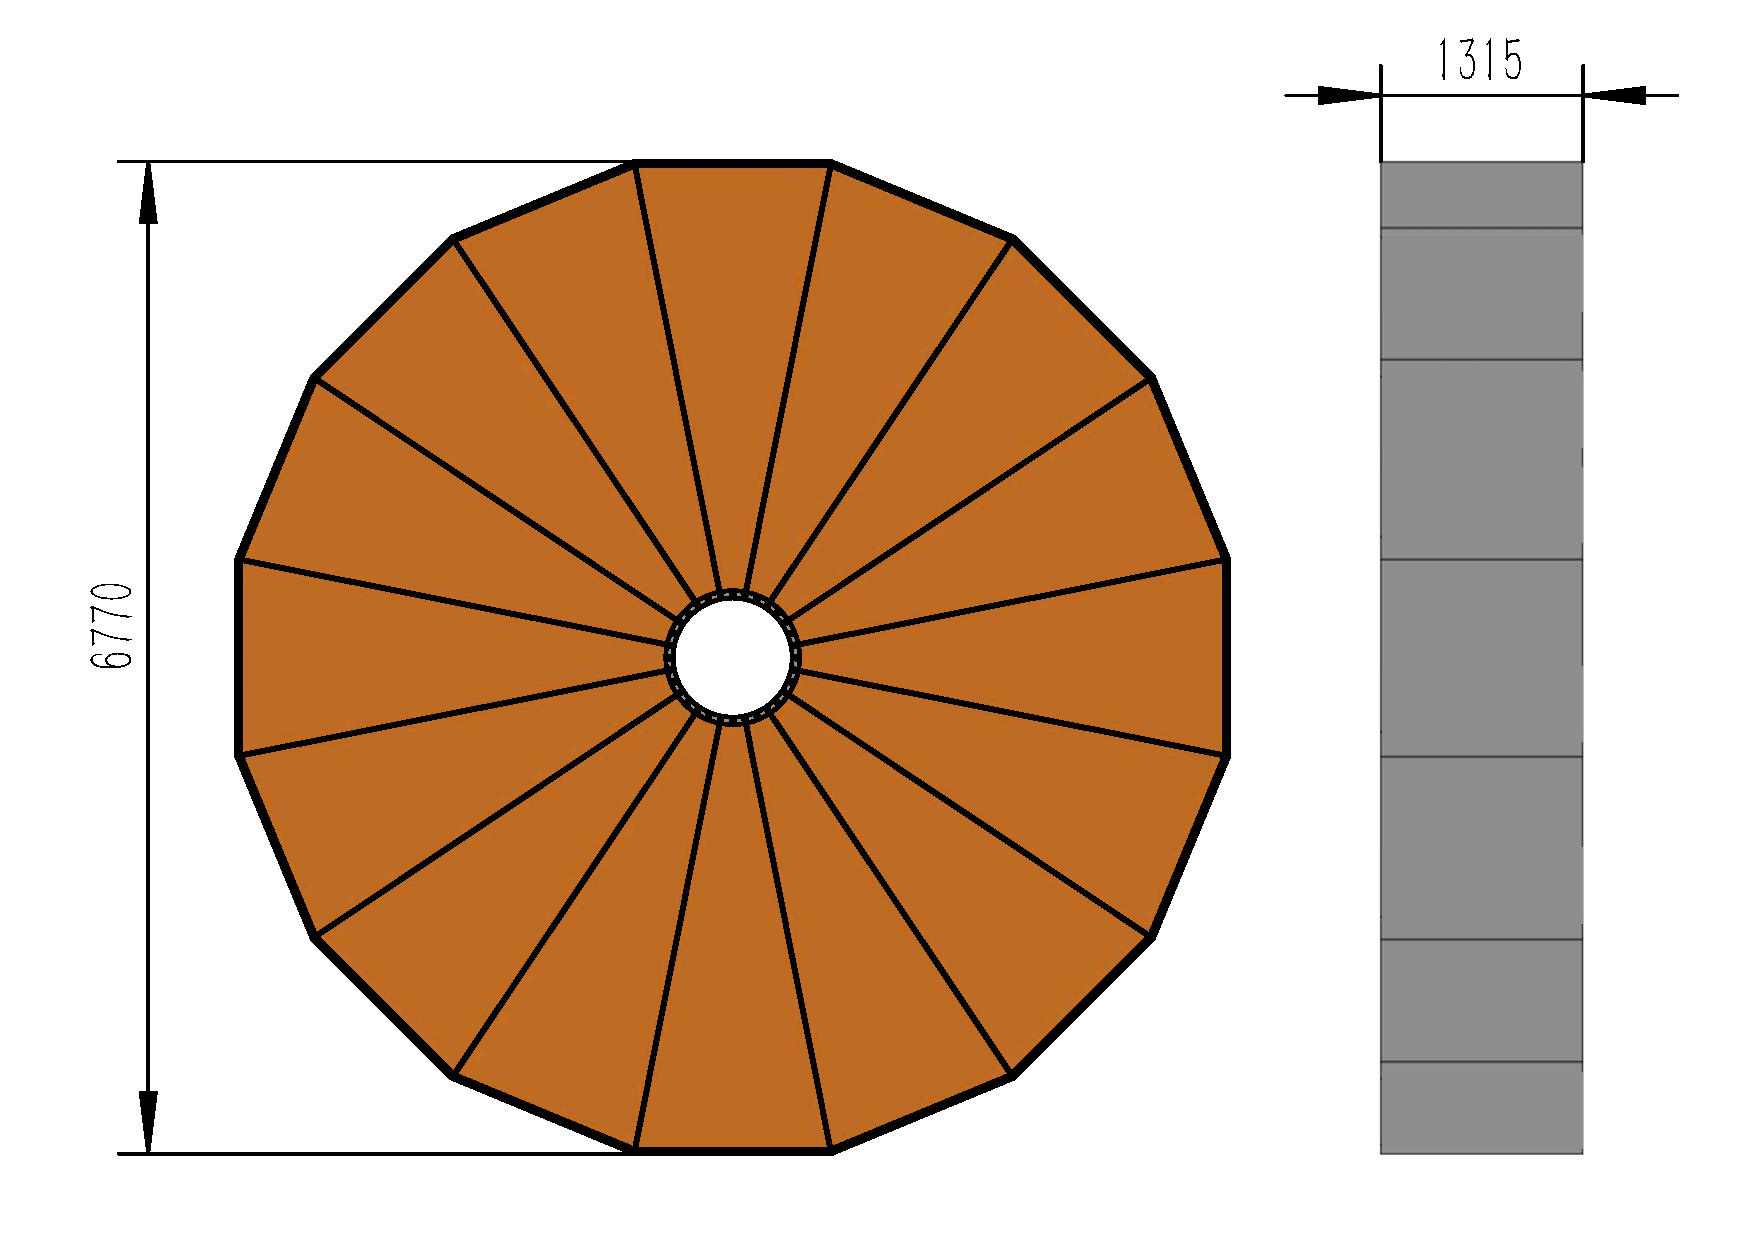
\includegraphics[width=\linewidth]{HCALEndcapOverall.pdf}
  \caption{}
\end{subfigure}\hfill
\begin{subfigure}{0.20\linewidth}
  \centering
  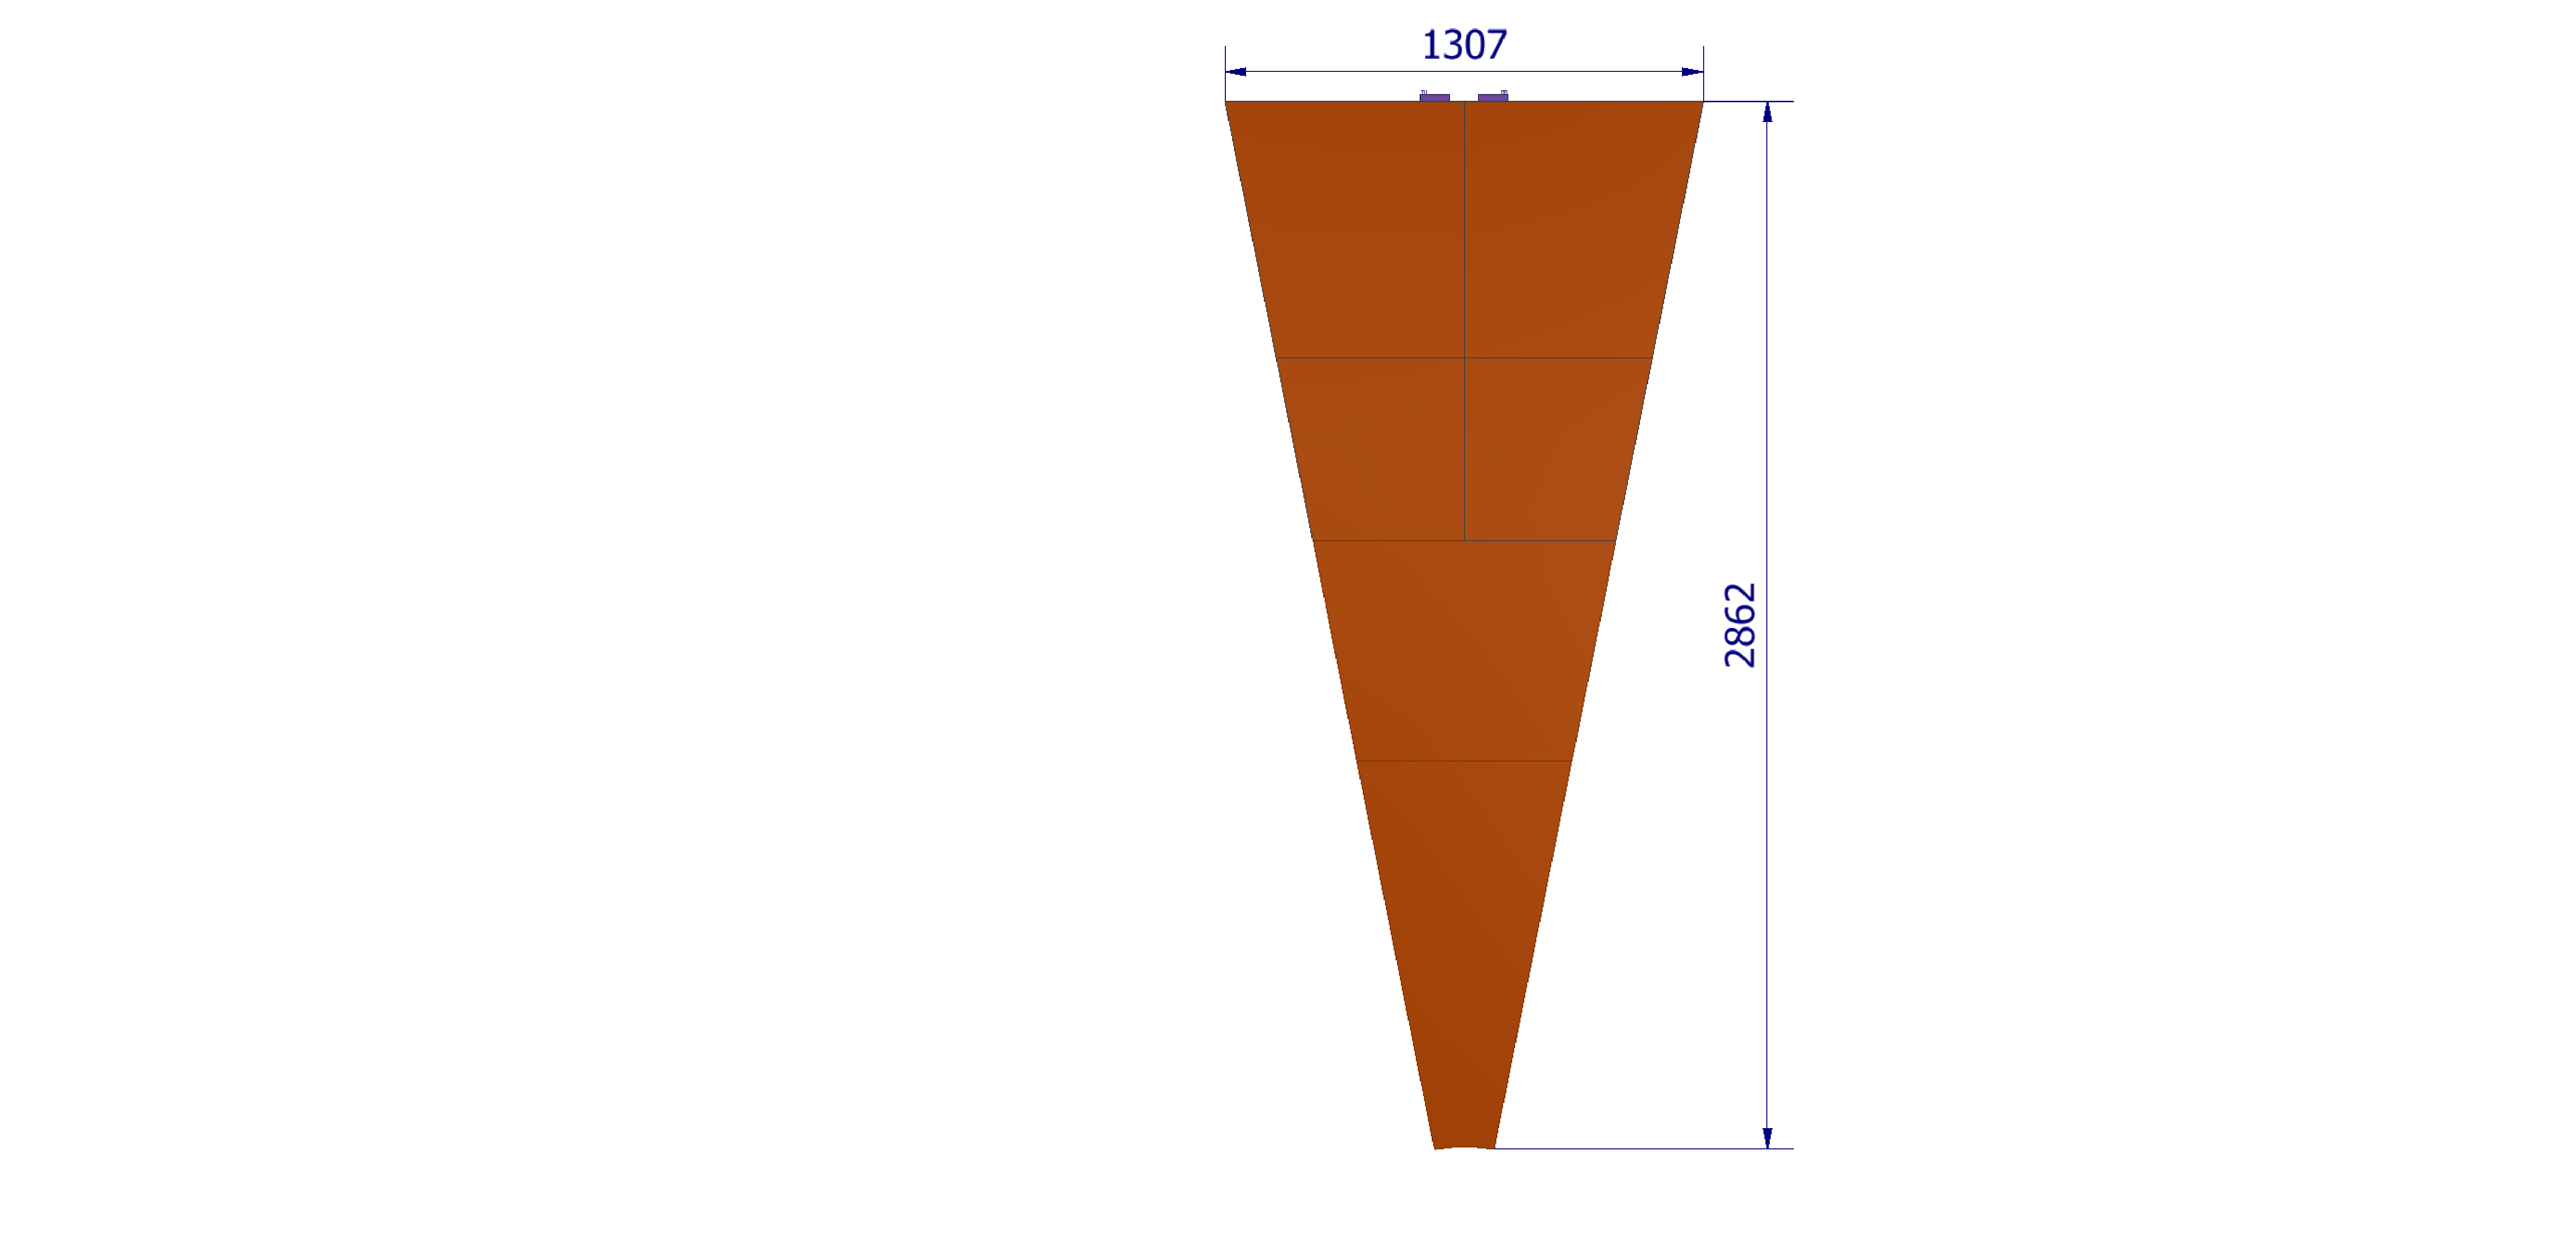
\includegraphics[width=\linewidth]{HCALEndcapOneSector.pdf}
  \caption{}
\end{subfigure}
\caption{Dimensions of the GS-HCAL endcaps.
(a)~Front and side views.
(b)~A single endcap sector.}
\label{fig:EndcapsOverall}
\end{figure}

%% --------------------------------------------------------------------
\subsection{Services: cooling, routing, and modular assembly}
\label{subsec:cooling}
%% --------------------------------------------------------------------

Service integration is an integral part of the baseline concept
because the 5.22~million channels and \SI{15}{mW/channel} ASIC power
impose non-trivial thermal and routing constraints on any practical
realisation.
A water-cooling system manages the front-end thermal load.
In the barrel, four cooling pipes are embedded in the steel absorber
of each layer, and every eight consecutive layers share common
manifolds to form six independent cooling loops per sector
(Figure~\ref{fig:BarrelCooling}).
In the endcap, 16~cooling regions per layer connect vertically across
all 48~layers to form 48~parallel circuits
(Figure~\ref{fig:M-14}).
The modular box architecture, combined with the eight-in-one cooling
topology, also provides clear routing paths for cables and gas, and
supports in-layer access during assembly and maintenance.

\begin{figure}[htbp]
\centering
\begin{subfigure}{0.55\linewidth}
  \centering
  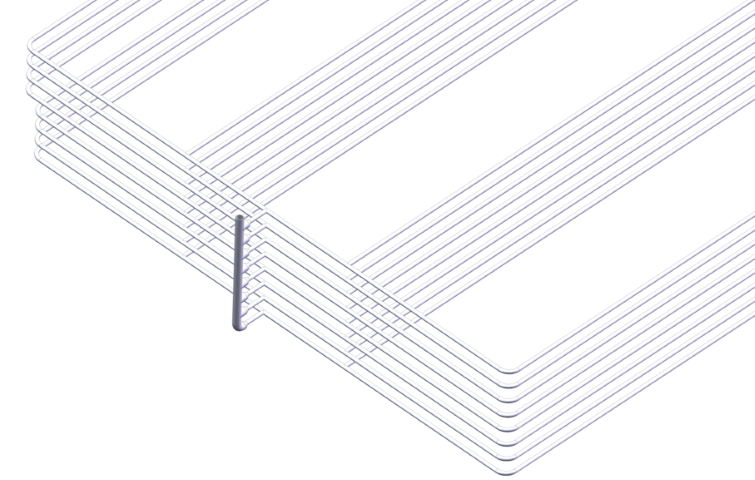
\includegraphics[width=\linewidth]{CoolingBarrelLeft.png}
  \caption{}
\end{subfigure}\hfill
\begin{subfigure}{0.35\linewidth}
  \centering
  \includegraphics[width=\linewidth]{CoolingBarrelv2.jpg}
  \caption{}
\end{subfigure}
\caption{Cooling-pipe routing for a barrel sector.
(a)~Schematic of the eight-in-one pipeline design.
(b)~Simulated coolant flow-velocity distribution.}
\label{fig:BarrelCooling}
\end{figure}

\begin{figure}[htbp]
\centering
\begin{subfigure}{0.50\linewidth}
  \centering
  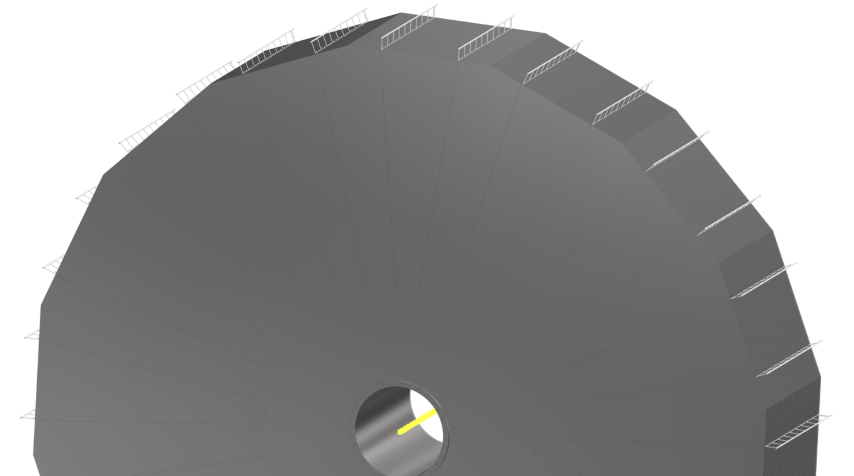
\includegraphics[width=\linewidth]{CoolingEndcapHalf.png}
  \caption{}
\end{subfigure}\hfill
\begin{subfigure}{0.42\linewidth}
  \centering
  \raisebox{0.1cm}{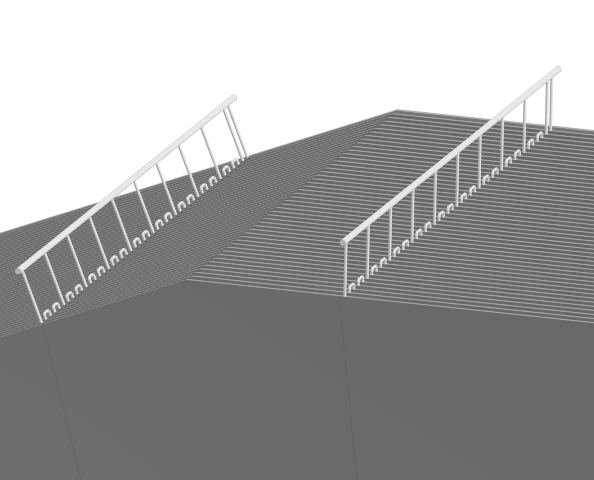
\includegraphics[width=\linewidth]{CoolingEndcapPart.png}}
  \caption{}
\end{subfigure}
\caption{Endcap cooling-pipe structure: (a)~half of the endcap;
(b)~zoomed corner view.}
\label{fig:M-14}
\end{figure}

%% --------------------------------------------------------------------
\subsection{Channel count and detector-scale implications}
\label{subsec:channels}
%% --------------------------------------------------------------------

Table~\ref{tab:GSHCALQuantities} summarises the cell, box, layer, and
sector counts.
The complete detector contains approximately 5.22~million readout
channels.
This number is itself a baseline-level design constraint:
it fixes the scale of ASIC production, calibration infrastructure
(Section~\ref{subsec:calibration}), and modular assembly
(Section~\ref{subsec:prototype}), and it is the principal driver of the
low-power per-channel requirement.
The baseline numbers are therefore chosen so that each of these
detector-scale dependencies is simultaneously feasible rather than
optimised independently.

\begin{table}[htbp]
\centering
\caption{Numbers of cells, boxes, layers, and sectors for the barrel
and the two endcaps.}
\label{tab:GSHCALQuantities}
\begin{tabular}{lcccc}
\toprule
\textbf{Part} & \textbf{Cells} & \textbf{Boxes} & \textbf{Layers} &
\textbf{Sectors} \\
\midrule
Barrel             & 3\,212\,800          & 27\,840        & $48\times16$
& 16 \\
Endcap ($\times2$) & $1\,006\,080\times2$ & $3072\times2$  &
$48\times16\times2$ & $16\times2$ \\
\bottomrule
\end{tabular}
\end{table}

%% ====================================================================
\section{Glass scintillator, photosensor, and front-end implementation}
\label{sec:activeunit}
%% ====================================================================

The baseline active unit---the GFO cell, the SiPM, the front-end
electronics, and the supporting optical simulation---constitutes the
primary technology chain of the GS-HCAL.
Each component is characterised as part of this integrated chain,
because the performance of any element is meaningful only in the
context of the others.

%% --------------------------------------------------------------------
\subsection{Choice of GFO glass as the baseline active medium}
\label{subsec:gfo}
%% --------------------------------------------------------------------

High-$Z$ glass scintillators have been investigated for calorimetry
since the 1980s~\cite{Buchner:1988fu}, but early attempts were limited
by short radiation length, low light yield, and strong self-absorption
in long-bar geometries.
The maturation of SiPM technology and PFA-oriented highly granular
calorimetry changed this picture: compact optically isolated cells of
${\sim}\SI{1}{cm}$-scale thickness eliminate the long-path
self-absorption problem, so that a moderate light yield of
${\sim}\SI{1000}{\phMeV}$ combined with a modern SiPM becomes
sufficient for practical readout~\cite{Tang:2022yrb,Hu:2023dbm,
Hu:2024nvo}.

Building on this opportunity, the Glass-Scintillator Collaboration has
systematically developed high-$Z$ glass
compositions~\cite{LAN2022113000,YU2023113846,ZHU2024} targeting the
density--light-yield trade-off with manufacturability at the
\cellsize cell scale (Figure~\ref{fig:GSGroup}).
Gadolinium fluoro-oxide (GFO) glass is adopted as the baseline active
medium because it combines high density, manufacturable tile geometry,
and adequate optical properties in a single
material~\cite{HUA202523367,Hua:2023myf,Hua:2024djh}.
Its key parameters are listed in Table~\ref{tab:GS1} alongside BGO
crystal~\cite{BGO} and DSB glass~\cite{Dormenev:2021vtn} for
reference.
GFO achieves a density of \SI{6.0}{g/cm^{3}} with a radiation length of
\SI{1.59}{cm} and a nuclear interaction length of \SI{24.2}{cm}.
The Ce$^{3+}$ luminescent centre provides strong emission near
\SI{400}{nm} with efficient energy transfer from Gd$^{3+}$
modifiers~\cite{GS-1}; the borosilicate matrix provides thermal and
optical stability; and the use of gadolinium, rather than lanthanum or
lutetium, provides a favourable combination of density, intrinsic
radioactivity, and cost.
These properties are directly matched to the \cellsize cell
requirement.

\begin{figure}[htbp]
\centering
\includegraphics[width=0.7\textwidth]{GSGroup.pdf}
\caption{Light yield versus density for GS samples developed by the
Glass-Scintillator Collaboration and by other groups.}
\label{fig:GSGroup}
\end{figure}

\begin{table}[htbp]
\centering
\caption{Key parameters of GFO glass ($5\times5\times5$~mm$^{3}$
sample) compared with BGO crystal~\cite{BGO} and DSB
glass~\cite{Dormenev:2021vtn}.}
\label{tab:GS1}
\begin{tabular}{lccc}
\toprule
\textbf{Parameter} & \textbf{GFO} & \textbf{BGO} & \textbf{DSB} \\
\midrule
Density (g/cm$^{3}$)                       & 6.0      & 7.13  & 4.2   \\
Melting point ($^{\circ}$C)                 & 1250     & 1050  & 1550  \\
Radiation length (cm)                       & 1.59     & 1.12  & 2.62  \\
Moli\`{e}re radius (cm)                    & 2.49     & 2.23  & 3.33  \\
Nuclear interaction length (cm)             & 24.2     & 22.7  & 31.8  \\
$Z_{\mathrm{eff}}$                          & 56.6     & 71.5  & 49.7  \\
$dE/dx$ (MeV/cm)                            & 8.0      & 8.99  & 5.9   \\
Emission peak (nm)                          & 400      & 480   & 430   \\
Refractive index                            & 1.74     & 2.15  & ---   \\
Light yield (ph/MeV)                        & ${\sim}1500$ & 7500  & 2500  \\
Energy resolution (\% at \SI{662}{keV})     & ${\sim}23$   & 9.5   & ---   \\
Scintillation decay time (ns)               & ${\sim}60$, 500 & 60, 300 & 90, 400 \\
\bottomrule
\end{tabular}
\end{table}

%% --------------------------------------------------------------------
\subsection{Optical constraints and attenuation length}
\label{subsec:attenuation}
%% --------------------------------------------------------------------

The light attenuation length (LAL, $L_{0}$) is the key optical
parameter that determines whether a given cell geometry is viable for
SiPM readout at the centre of the cell.
The LAL is measured by thickness-dependent transmittance using
\begin{equation}
\label{eq:LAL}
L_{0} = \frac{L_{2}-L_{1}}{\ln(T_{L_{1}}/T_{L_{2}})},
\end{equation}
with two sample thicknesses $L_{1}<L_{2}$ and transmittances
$T_{L_{i}}$~\cite{Zhu:1996tt}.
The best-performing GFO sample yields
$L_{0}\approx\SI{6}{cm}$ at \SI{400}{nm}, the GS emission peak, and
remains between \SI{6}{cm} and \SI{6.8}{cm} across the visible
spectrum (Figure~\ref{fig:newLAL1}).

This value is compatible with the \cellsize baseline cell geometry.
The SiPM is mounted at the centre of the cell top surface, and the
longest straight optical path from a scintillation point to the sensor
is bounded by the cell diagonal,
$\sqrt{20^{2}+20^{2}+10^{2}}\approx\SI{30}{mm}$.
This is a factor of two smaller than the measured LAL, so first-pass
photon transport is dominated by geometric acceptance and Teflon
reflection rather than by bulk absorption.
The baseline attenuation length is therefore adequate for the cell
geometry; it does not require the centimetre-scale improvements that
would be mandatory in a long-bar readout.

\begin{figure}[htbp]
\centering
\includegraphics[width=0.60\textwidth]{NewLAL1.pdf}
\caption{Attenuation length of GFO glass versus wavelength, measured
using the transmittance method.}
\label{fig:newLAL1}
\end{figure}

%% --------------------------------------------------------------------
\subsection{SiPM selection and compatibility with the baseline cell}
\label{subsec:sipm}
%% --------------------------------------------------------------------

Silicon photomultipliers (SiPMs) are selected for the GS-HCAL readout
because of their compact form factor, high gain at low operating
voltage, radiation hardness, and insensitivity to magnetic fields.
They are already deployed in the CMS High-Granularity
Calorimeter~\cite{CMS:2017jpq} and CALICE highly granular
prototypes~\cite{calice}.
Four representative commercial devices from HPK, NDL, and JBT are
compared in Table~\ref{tab:SiPM-tab1}.

\begin{table}[htbp]
\centering
\caption{Parameters of commercial SiPMs evaluated for the GS-HCAL\@.}
\label{tab:SiPM-tab1}
\resizebox{\textwidth}{!}{%
\begin{tabular}{lcccc}
\toprule
\textbf{Supplier} & \multicolumn{2}{c}{\textbf{HPK}} &
\textbf{NDL} & \textbf{JBT} \\
\midrule
Type  & S14160-3015PS & S14160-3050HS & EQR20-11-3030-S & JSP-TP3050-SMT \\
Pixel pitch ($\upmu$m) & 15 & 50 & 20 & 50 \\
Number of pixels & 39\,984 & 3531 & 22\,500 & 3364 \\
Terminal capacitance (pF) & 530 & 500 & 157.5 & 0.170 \\
Breakdown voltage (V)
  & $38\pm3$ & $38\pm3$ & $27.2\pm1$ & $24.6\pm0.2$ \\
Recommended $V_{\mathrm{op}}$ (V)
  & $V_{\mathrm{BD}}+3$ & $V_{\mathrm{BD}}+2.7$
  & $V_{\mathrm{BD}}+5$ & $V_{\mathrm{BD}}+2$ \\
Peak-sensitivity wavelength (nm) & 450 & 450 & 420 & 420 \\
Peak PDE (\%) & 32 & 50 & 47.8 & 35 \\
PDE at \SI{400}{nm} (\%) & 27 & 47 & 45 & 33 \\
Gain & $3.6\times10^{5}$ & $2.5\times10^{6}$
     & $8.0\times10^{5}$ & $2.1\times10^{6}$ \\
DCR (kHz/mm$^{2}$) & 700--2100 & 10--100 & 150--450 & 120--270 \\
\bottomrule
\end{tabular}}
\end{table}

The selection is driven by four properties matched to the baseline
cell: high PDE at \SI{400}{nm} (matching the GFO emission peak);
sufficient gain for resolved photon counting; low dark count rate
(DCR); and cost compatible with millions of channels.

The central question for SiPM compatibility with the baseline cell is
whether the measured cell light output is large enough that a
threshold sufficient to suppress DCR can still be set well below one
MIP.
Figure~\ref{fig:ch08_SiPM_DCR} shows the DCR as a function of
photoelectron threshold for the candidate SiPMs.
With a measured cell output of ${\sim}60$~\peMIP, a \SI{0.1}{MIP}
threshold corresponds to approximately six photoelectrons.
At this threshold the DCR drops to approximately \SI{28}{Hz/mm^{2}}
(NDL~EQR20) and \SI{12}{Hz/mm^{2}} (HPK~S14160-3050)---well below the
expected hadronic event rate---demonstrating that the baseline cell
and commercial SiPMs together provide a practical
signal-to-noise margin.
The HPK~S14160-3050 and NDL~EQR20-11-3030 are therefore identified as
the most promising devices for the prototype phase.

\begin{figure}[htbp]
\centering
\includegraphics[width=0.60\textwidth]{SiPM_DCR_HCAL.pdf}
\caption{Dark count rate versus threshold level for several SiPM
models.}
\label{fig:ch08_SiPM_DCR}
\end{figure}

%% --------------------------------------------------------------------
\subsection{Front-end readout concept}
\label{subsec:fee}
%% --------------------------------------------------------------------

The baseline readout must eventually handle more than five million
SiPM channels with a dynamic range of 0.1--100~MIP, a charge
resolution of 10\% of 1~MIP, and an average event rate of
\SI{2}{kHz/channel}.
The resulting system-level requirements are summarised in
Table~\ref{tab:SiPM-tab3}.
A dedicated low-power ASIC meeting these specifications is under
development; it is one of the items that are expected to close with
the prototype.

\begin{table}[htbp]
\centering
\caption{SiPM-driven requirements for the readout electronics.}
\label{tab:SiPM-tab3}
\begin{tabular}{ll}
\toprule
\textbf{Parameter} & \textbf{Requirement} \\
\midrule
Charge dynamic range       & \SI{0.8}{pC}--\SI{800}{pC} (0.1--100~MIP) \\
Charge resolution          & 10\% of 1.0~MIP \\
SiPM capacitance           & $\leq\SI{100}{pF}$ \\
SiPM gain                  & $\geq5\times10^{5}$ \\
Average event rate/channel & \SI{2}{kHz} \\
Maximum event rate/channel & \SI{50}{kHz} \\
Typical signal amplitude   & 2--3~mV/p.e. \\
\bottomrule
\end{tabular}
\end{table}

For single-cell characterisation and prototype testing an interim
front-end solution was developed, because no commercial option
simultaneously met the baseline requirements~\cite{Wang:2023ffl}.
The interim pre-amplifier achieves a gain of $\pm\SI{20}{V/V}$, a
bandwidth of \SI{400}{MHz}, and a baseline noise of
$300\,\mu\mathrm{V}_\mathrm{RMS}$ at \SI{50}{\ohm} input impedance
(Figure~\ref{fig:SiPM_FEE}); this is sufficient to resolve
single-photoelectron peaks and to support all the single-cell
measurements of Section~\ref{sec:expchar}.

\begin{figure}[htbp]
\centering
\includegraphics[width=0.95\textwidth]{SiPM_FEE.pdf}
\caption{Pre-amplifier for the GS-HCAL SiPM readout.
(a)~Single-channel PCB coupled to a GS cell.
(b)~Schematic diagram.
(c,\,d)~Performance characteristics.
(e)~Waveform of a \sipmsize NDL SiPM (EQR20-11-3030D-S).
(f)~ADC spectrum of SiPM dark noise with well-separated
photoelectron peaks.}
\label{fig:SiPM_FEE}
\end{figure}

%% --------------------------------------------------------------------
\subsection{Optical simulation as design support}
\label{subsec:optsim}
%% --------------------------------------------------------------------

Geant4-based optical simulation~\cite{Tang:2022yrb} of a single
GS~cell coupled to a SiPM is used to support the design choices.
The simulation implements the baseline \cellsize cell with a single
\sipmsize SiPM at its centre, with the cell periphery wrapped in
Teflon reflective film; the physics list \texttt{QGSP\_BERT} is
combined with a full set of optical processes including scintillation,
Cherenkov radiation, Rayleigh scattering, bulk absorption, and
boundary effects.
Figure~\ref{fig:SiPM_MIPmap}(a) shows the simulated light-output
distribution for a cell with \SI{60}{mm} attenuation length, yielding
$42.05\pm0.01$~\peMIP; Figure~\ref{fig:SiPM_MIPmap}(b) shows the
expected dependence of the light output on the attenuation length
across 40, 60, and \SI{80}{mm}.

\begin{figure}[htbp]
\centering
\begin{subfigure}{0.43\textwidth}
  \centering
  \includegraphics[width=\linewidth]{Muon_GS_map_PDE60_3time3_AT6cmPE.pdf}
  \caption{}
\end{subfigure}\hfill
\begin{subfigure}{0.39\textwidth}
  \centering
  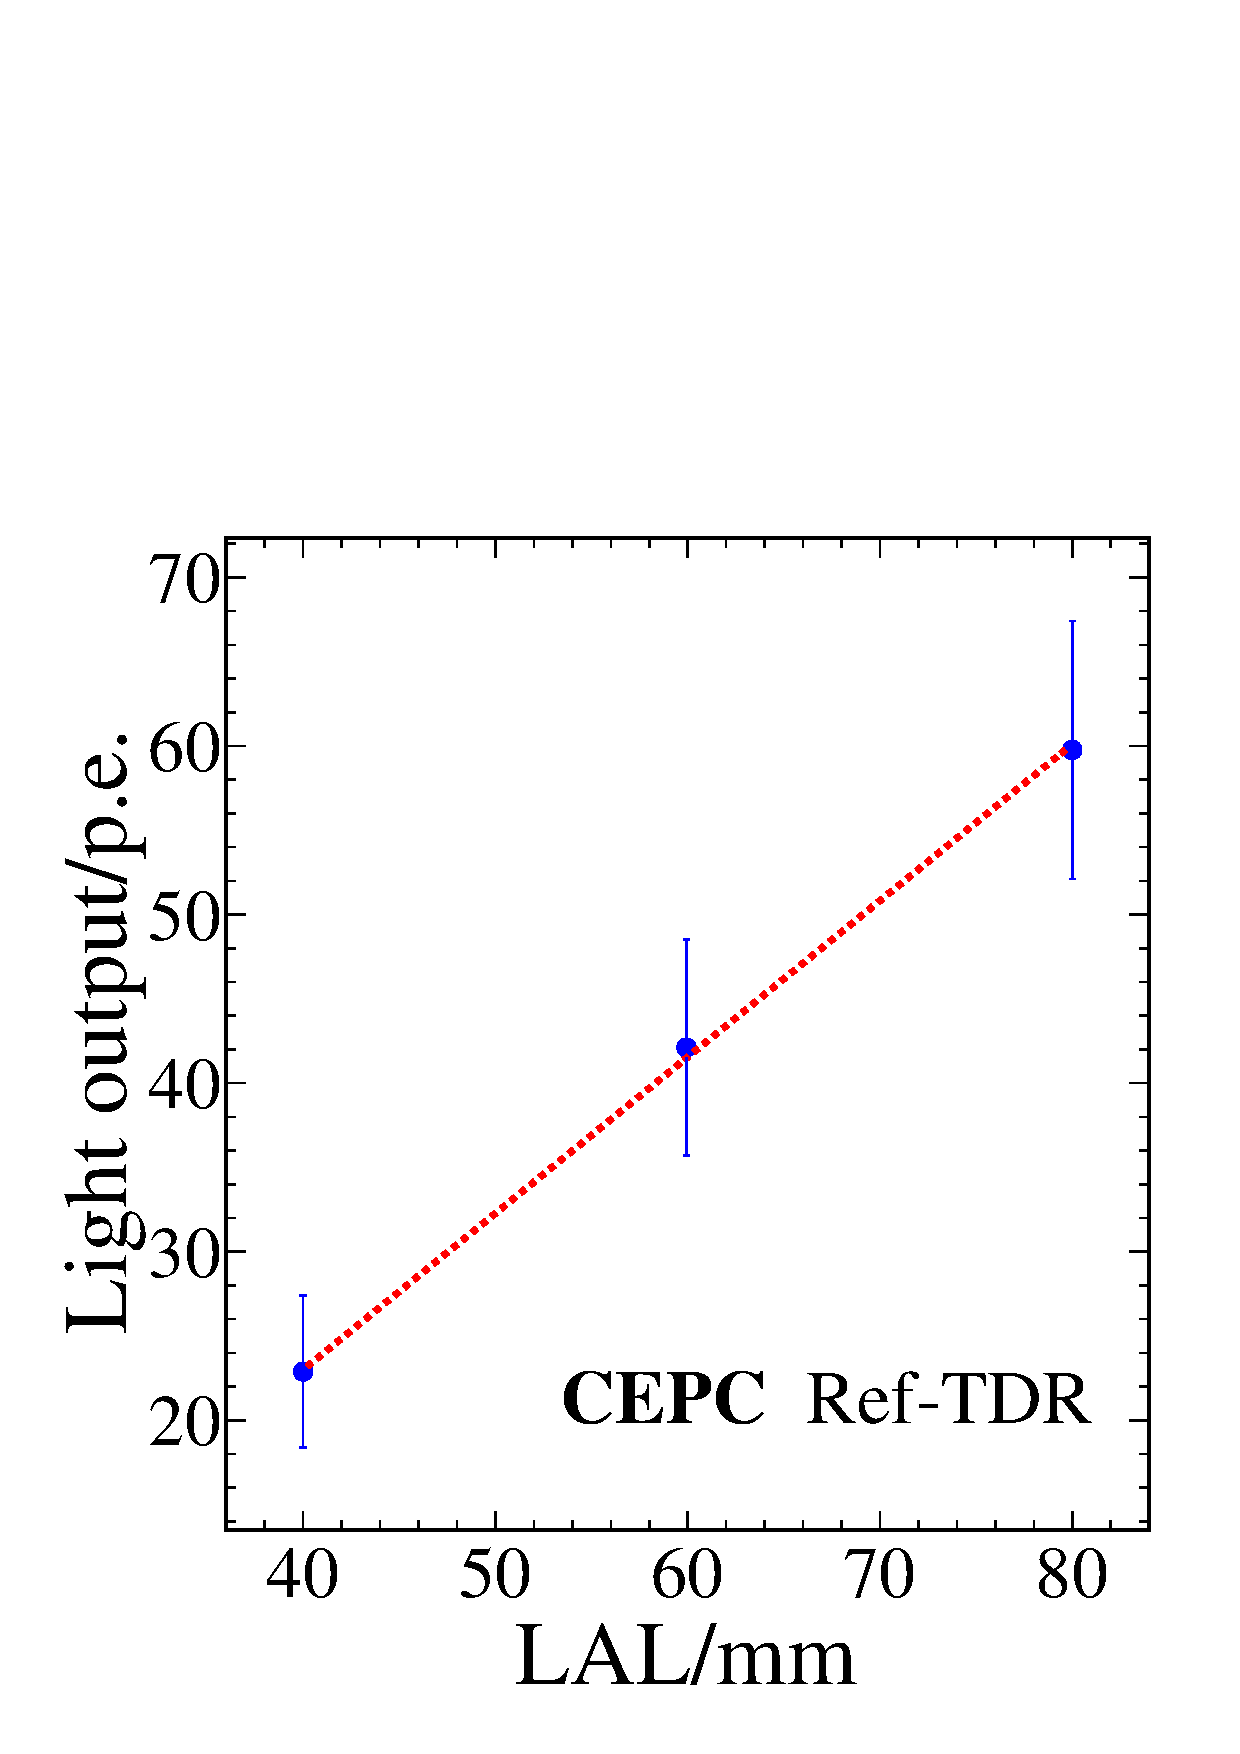
\includegraphics[width=\linewidth]{attenuation_fit.pdf}
  \caption{}
\end{subfigure}
\caption{(a)~Simulated light-output distribution of a GS cell with
\SI{60}{mm} attenuation length ($42.05\pm0.01$~\peMIP).
(b)~Fitted light-output MPV versus attenuation length.}
\label{fig:SiPM_MIPmap}
\end{figure}

Validation studies (Figure~\ref{fig:SiPM_SimValid}) show simulated
fast and slow scintillation components of \SI{96}{ns} and
\SI{1445}{ns}, somewhat longer than the measured reference values
of \SI{60}{ns} and \SI{500}{ns} (Table~\ref{tab:GS1}), and the
simulated single-muon light yield
(${\sim}\SI{42}{\peMIP}$) is lower than the measured cosmic-ray result
of ${\sim}\SI{64}{\peMIP}$ (Section~\ref{subsec:cellmeas}).
The optical simulation therefore plays a supporting role in the
baseline rationale rather than providing final experimental closure:
the current Geant4 optical model requires tuning against measured GFO
data, and this tuning is one of the immediate priorities of the
validation programme (Section~\ref{sec:discussion}).

\begin{figure}[htbp]
\centering
\begin{subfigure}{0.43\textwidth}
  \centering
  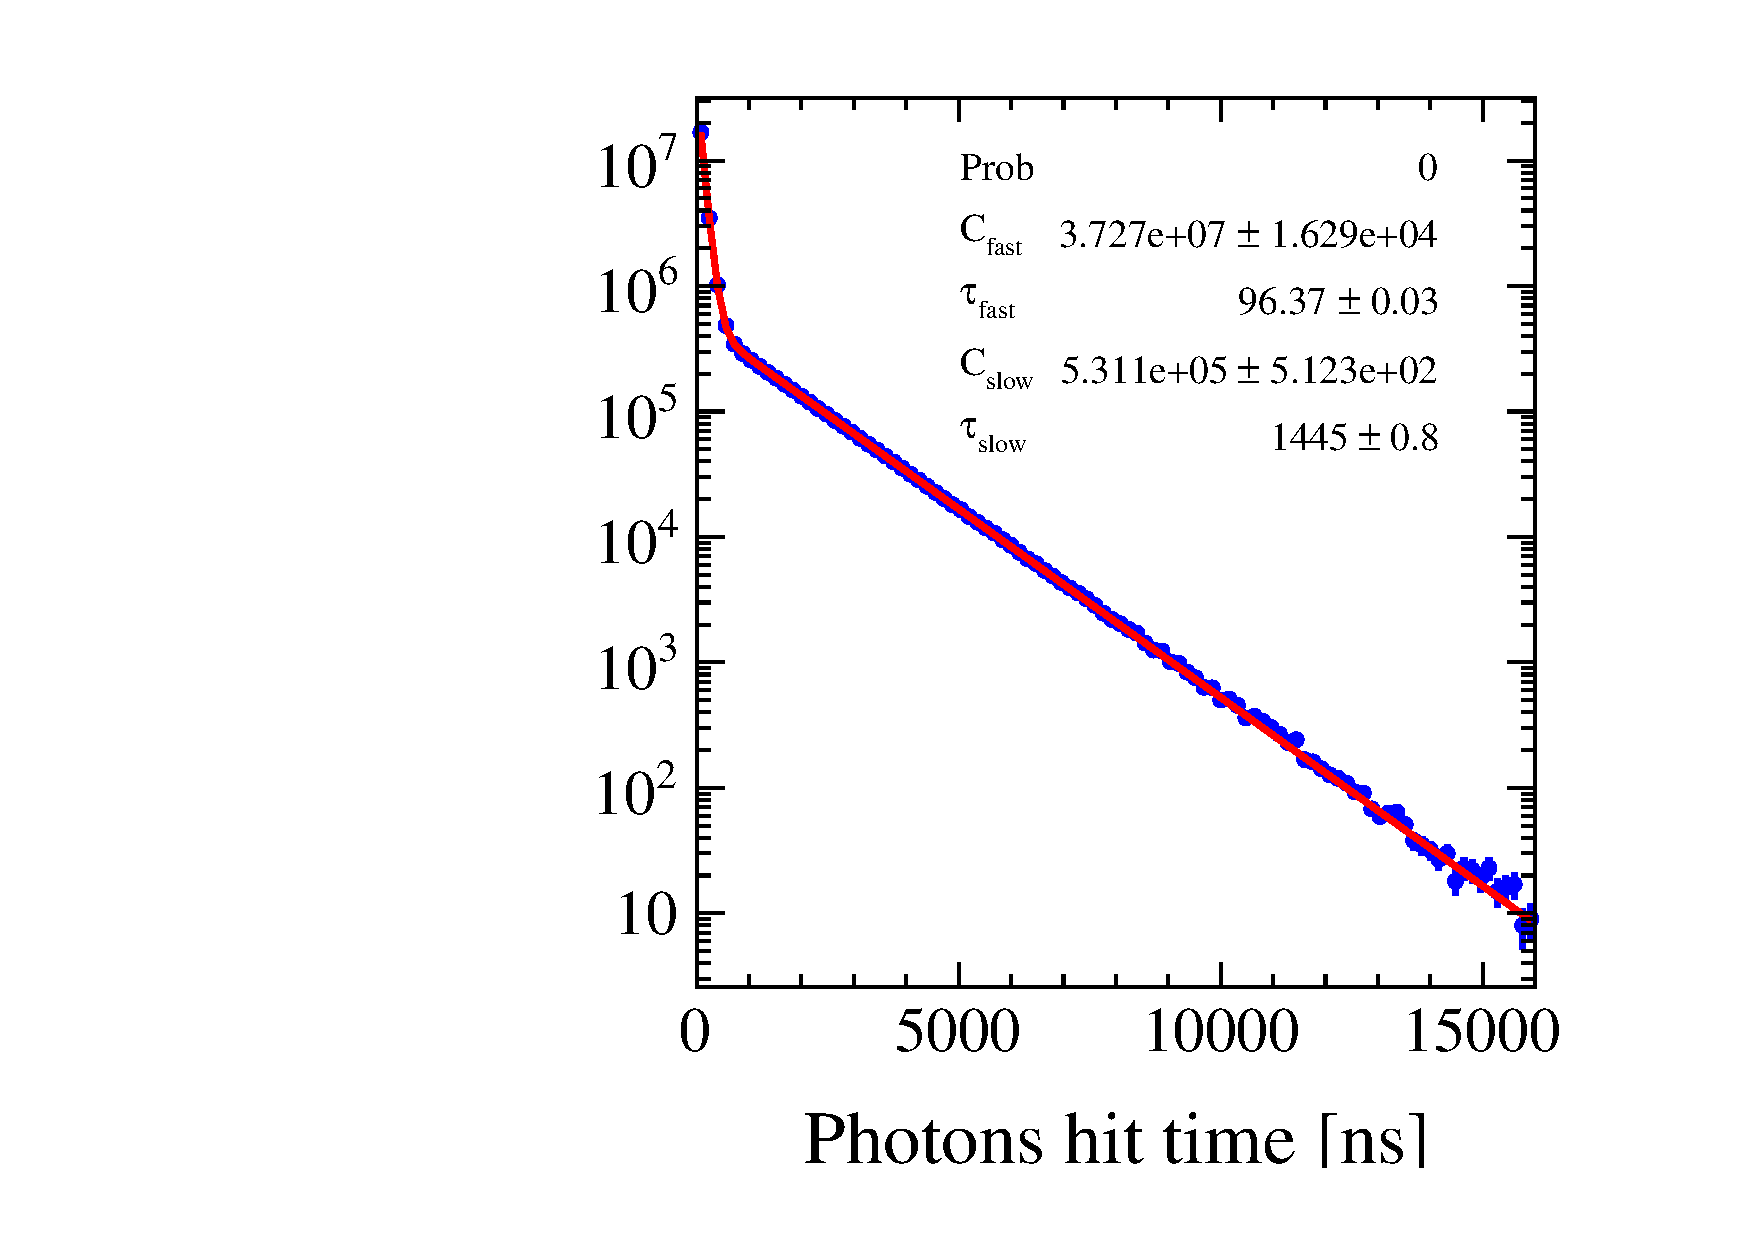
\includegraphics[width=\linewidth]{timeSpe.pdf}
  \caption{}
\end{subfigure}\hfill
\begin{subfigure}{0.38\textwidth}
  \centering
  \includegraphics[width=\linewidth]{Edp.pdf}
  \caption{}
\end{subfigure}
\caption{Simulation validation: (a)~scintillation-time distribution
(fast and slow components); (b)~muon deposited energy in a
\SI{10}{mm}-thick GS cell.}
\label{fig:SiPM_SimValid}
\end{figure}

%% ====================================================================
\section{Experimental characterisation of the baseline active unit}
\label{sec:expchar}
%% ====================================================================

The experimental evidence supporting the baseline active unit spans
four complementary measurement types.
The intrinsic light yield and optical response of the GFO glass
establish its suitability as the active medium.
Radiation-tolerance measurements confirm adequate performance under
CEPC-relevant doses.
Single-cell measurements with three independent probes---a
$^{137}$Cs source, cosmic-ray muons, and \SI{5}{GeV} electrons at
KEK---characterise the cell-level signal across the dynamic range of
interest.
Finally, initial tile-production studies address reproducibility and
quality control at batch scale.

%% --------------------------------------------------------------------
\subsection{Light yield and optical response}
\label{subsec:lightyield}
%% --------------------------------------------------------------------

Figure~\ref{fig:LargeGS} shows GFO glass cells of \cellsize under
natural and ultraviolet illumination.
Figure~\ref{fig:GS40}(a) shows the X-ray-excited luminescence (XEL)
and optical-transmission spectra of the GFO glass; the transmittance
in the visible range exceeds 80\%, with self-absorption observed near
the \SI{400}{nm} emission peak~\cite{SUI2025100878}.
Extensive $\gamma$-ray testing confirms that the GFO intrinsic light
yield consistently exceeds \SI{1000}{\phMeV}.
When measured with an XP2020 \SI{2}{inch} PMT, the GFO
photoelectron yield reaches approximately one-third that of BGO
crystals of identical dimensions~\cite{GS-5}
(Figure~\ref{fig:GS40}b).
Figure~\ref{fig:GS40}(c) shows the scintillation-decay profile under
$\gamma$-ray excitation: the slow-component decay time is below
\SI{500}{ns}, fully compatible with the high granularity and trigger
rate envisaged for the GS-HCAL.

Together these results establish the optical response required to
support the baseline cell: a light yield sufficient for
${\sim}60$~\peMIP readout, a transmittance compatible with bulk
photon transport across the cell, and a decay time compatible with
the baseline trigger window.

\begin{figure}[htbp]
\centering
\begin{subfigure}{0.40\textwidth}
  \centering
  \includegraphics[width=\linewidth]{GSN.pdf}
  \caption{}
\end{subfigure}\hfill
\begin{subfigure}{0.42\textwidth}
  \centering
  \includegraphics[width=\linewidth]{GSUV.pdf}
  \caption{}
\end{subfigure}
\caption{GFO glass cells of \cellsize under (a)~natural light and
(b)~ultraviolet illumination.}
\label{fig:LargeGS}
\end{figure}

\begin{figure}[htbp]
\centering
\begin{subfigure}{0.50\textwidth}
  \centering
  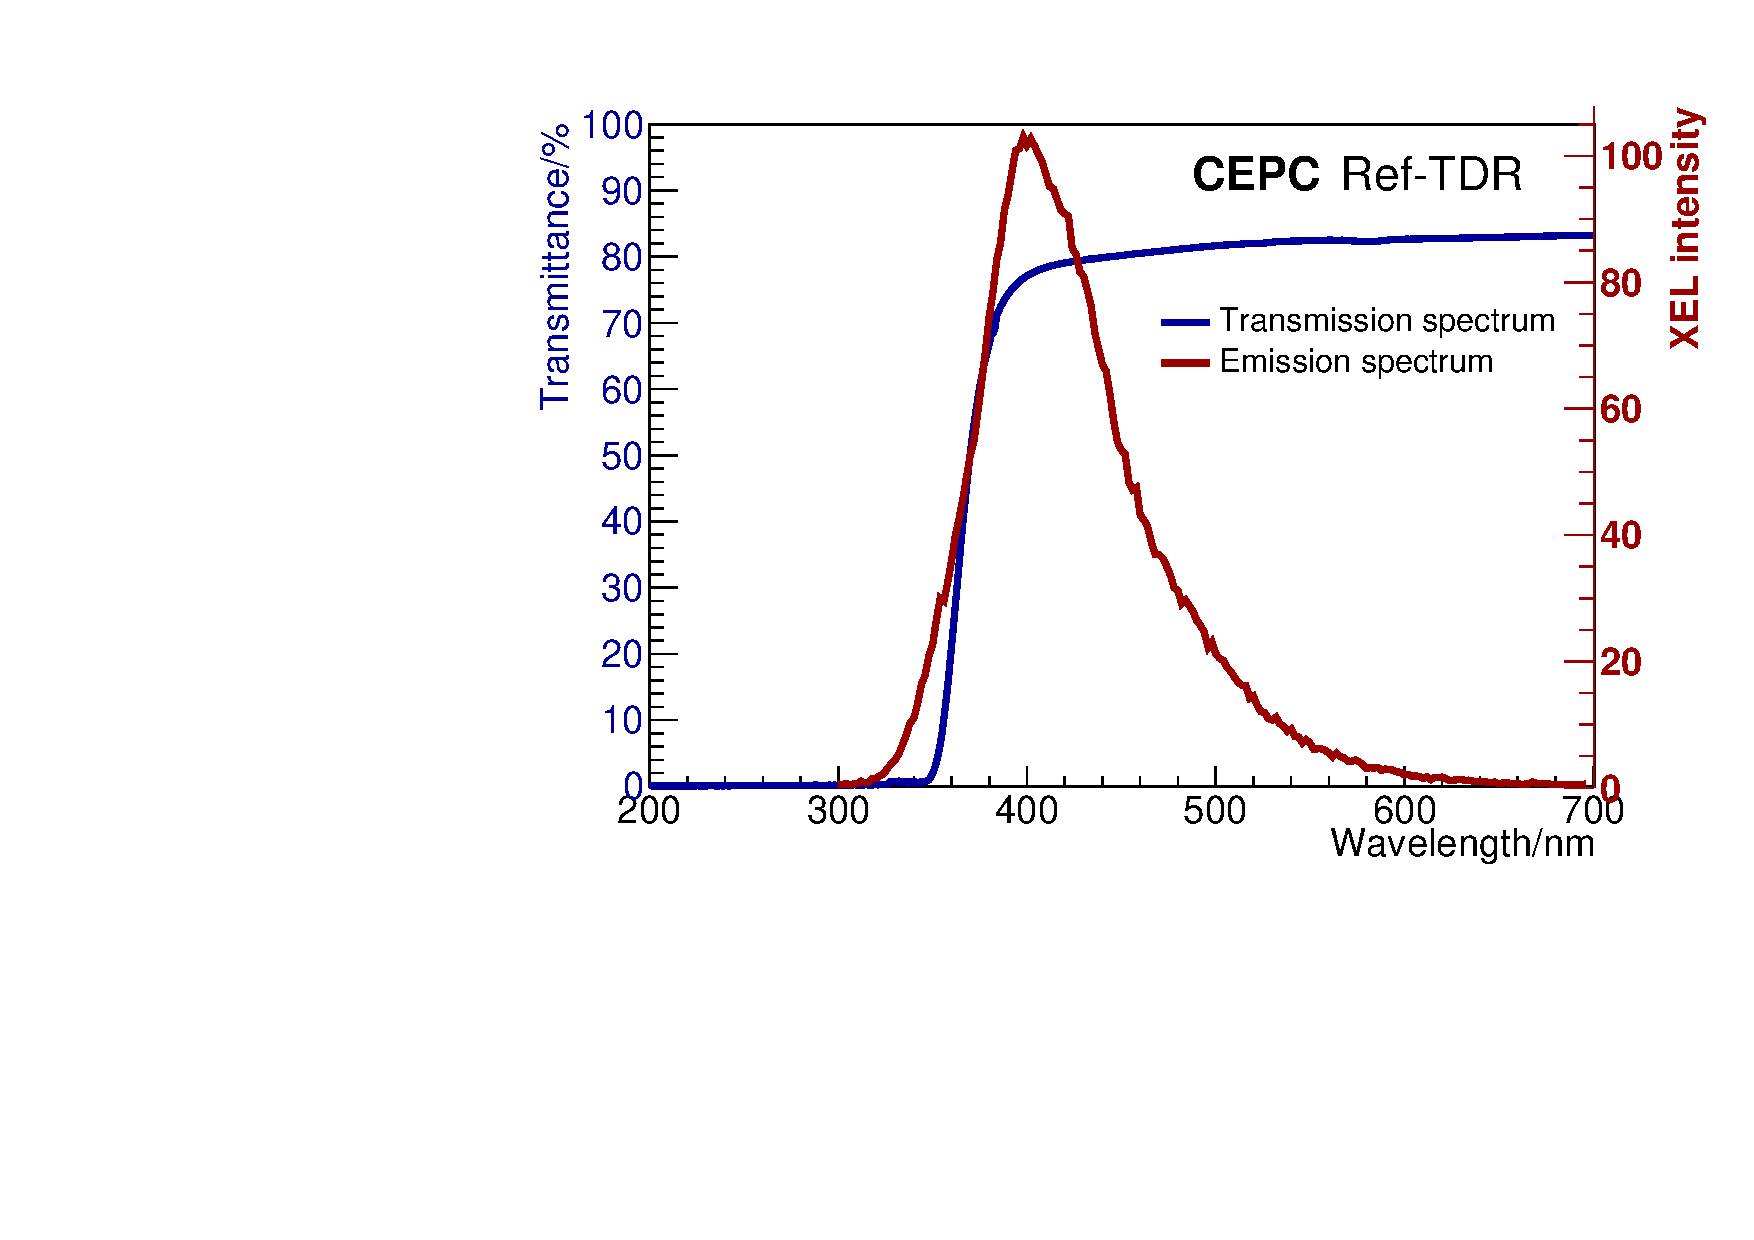
\includegraphics[width=\linewidth]{newGS40-A.pdf}
  \caption{}
  \label{fig:GS40-a}
\end{subfigure}

\vspace{0.3cm}

\begin{subfigure}{0.45\textwidth}
  \centering
  \includegraphics[width=\linewidth]{GS40-b.pdf}
  \caption{}
  \label{fig:GS40-b}
\end{subfigure}\hfill
\begin{subfigure}{0.45\textwidth}
  \centering
  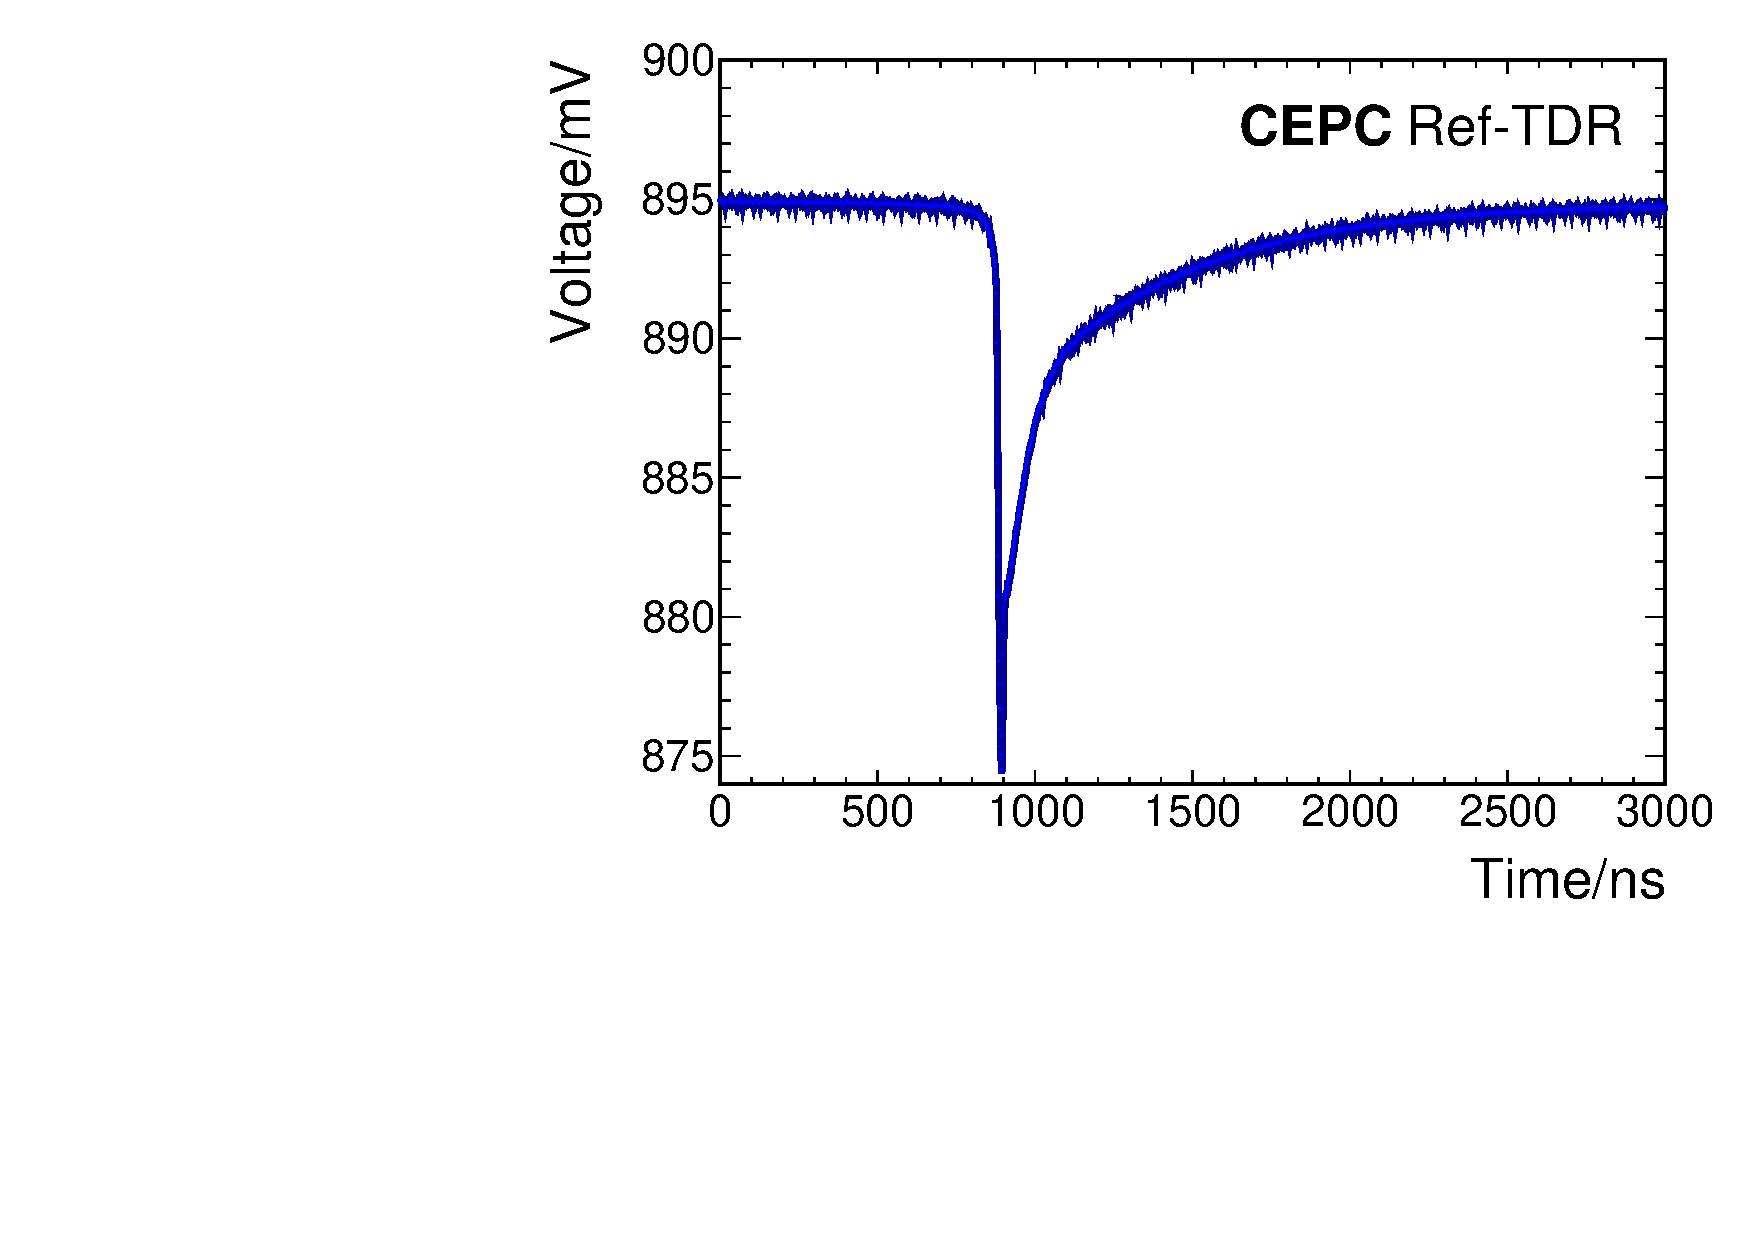
\includegraphics[width=\linewidth]{GS40-c.pdf}
  \caption{}
  \label{fig:GS40-c}
\end{subfigure}
\caption{(a)~Optical-transmission and XEL spectra of the GFO glass.
(b)~Energy spectra of GFO GS and BGO crystal of the same dimensions.
(c)~Scintillation decay curve of the GFO glass.}
\label{fig:GS40}
\end{figure}

%% --------------------------------------------------------------------
\subsection{Radiation tolerance under CEPC-relevant doses}
\label{subsec:radiation}
%% --------------------------------------------------------------------

Under the current CEPC operating plan, the accumulated radiation dose
reaches approximately \SI{40}{Gy} during the ten-year Higgs run at
$\mathcal{L}=8\times10^{34}$~cm$^{-2}$s$^{-1}$, and is estimated at
\SI{96}{Gy} per year during $Z$-pole operation at
$\mathcal{L}=192\times10^{34}$~cm$^{-2}$s$^{-1}$.
A dose benchmark of \SI{100}{Gy} therefore covers the practically
relevant operational range.

Figure~\ref{fig:gamma-irradiation} shows the relative light yield of
GFO glass as a function of $\gamma$-irradiation dose.
The retention exceeds 70\% at \SI{100}{Gy} (measured 71.2\%), and the
result is confirmed by proton-beam irradiation~\cite{YIN2026170869} at
the APEP facility~\cite{Liu:2022czi}.
These measurements demonstrate that the baseline active medium
preserves adequate optical response under CEPC-relevant doses.

\begin{figure}[htbp]
\centering
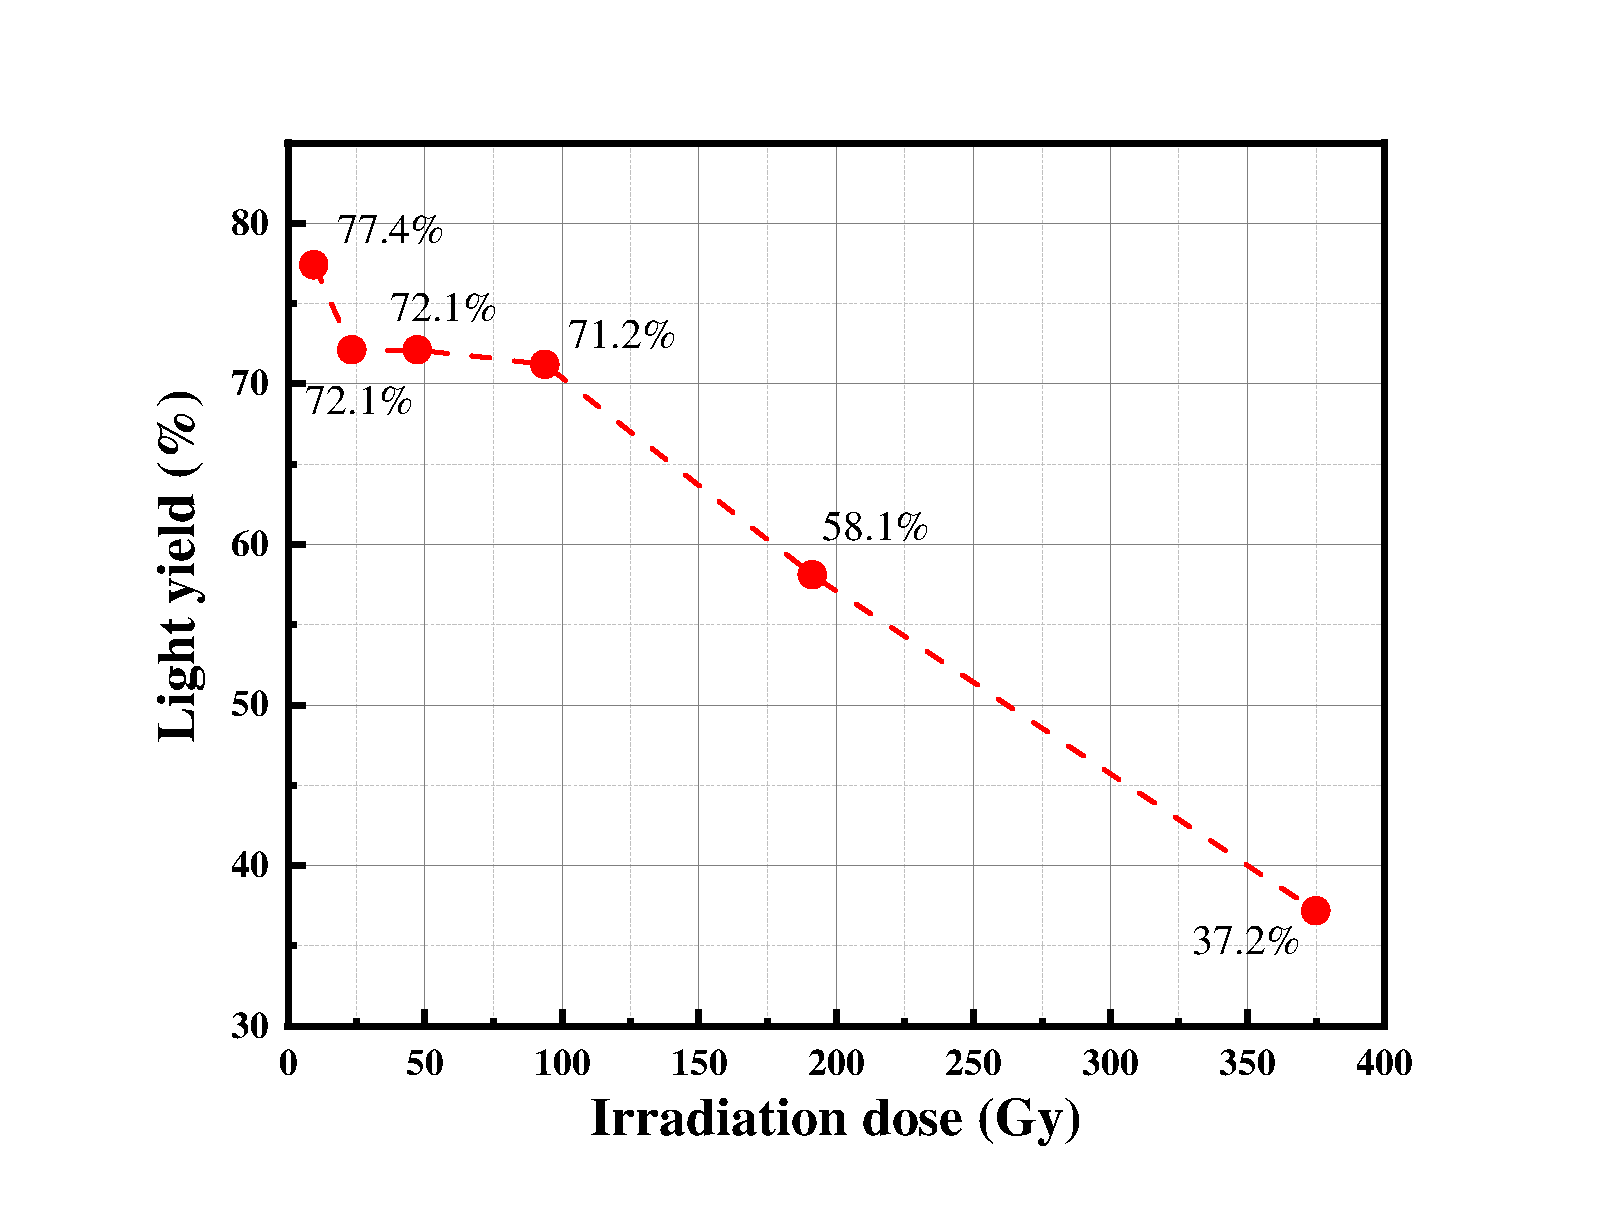
\includegraphics[width=0.60\linewidth]{LightYieldReductionGammaIrradiation.pdf}
\caption{Relative light yield of GFO glass as a function of
$\gamma$-irradiation dose.  At \SI{100}{Gy} the retention is 71.2\%.}
\label{fig:gamma-irradiation}
\end{figure}

%% --------------------------------------------------------------------
\subsection{Single-cell measurements with different probes}
\label{subsec:cellmeas}
%% --------------------------------------------------------------------

The effective light output of the \cellsize GS cell was evaluated in
three independent single-cell measurement campaigns using different
probes:
(i)~\SI{662}{keV} $\gamma$-rays from a $^{137}$Cs source;
(ii)~cosmic-ray muons with an expected energy deposition of
  \SI{7.7}{MeV/MIP};
(iii)~\SI{5}{GeV} electron beams at KEK.
In each case the SiPM was mounted at the cell centre on a readout
board with the interim pre-amplifier of Section~\ref{subsec:fee}.
Comparative tests of enhanced-specular-reflector (ESR) and Teflon
reflective films showed that Teflon provides approximately 20\%
higher effective reflectivity~\cite{Janecek:2012qit}, and all
measurements therefore employ Teflon wrapping.

\paragraph{$^{137}$Cs source.}
Using the HPK~S14160-3050HS SiPM (spectrum-weighted PDE~44.5\%), the
MPV for \SI{662}{keV} $\gamma$-rays is 12.9~p.e.;
scaled to a \SI{7.7}{MeV} MIP energy deposition this corresponds to an
equivalent light output of approximately 150~\peMIP.

\paragraph{Cosmic-ray muons.}
A trigger formed by two plastic-scintillator panels selects
through-going muons.
Using the HPK~S13360-3050PE SiPM (spectrum-weighted PDE~32.5\%), the
measured cell light output is $63.6\pm0.5$~\peMIP
(Figure~\ref{fig:SiPM_Celltest}b).

\paragraph{5~GeV electrons at KEK.}
A Landau fit to the electron spectrum measured with the
NDL~EQR20-11-3030 SiPM (spectrum-weighted PDE~42.5\%) yields an MPV of
$157.6\pm2.9$~\peMIP (Figure~\ref{fig:SiPM_Celltest}c).

\begin{figure}[htbp]
\centering
\begin{subfigure}{0.49\textwidth}
  \centering
  \includegraphics[width=\linewidth]{GS-SiPM-Cs137-Teflon.pdf}
  \caption{}
\end{subfigure}\hfill
\begin{subfigure}{0.49\textwidth}
  \centering
  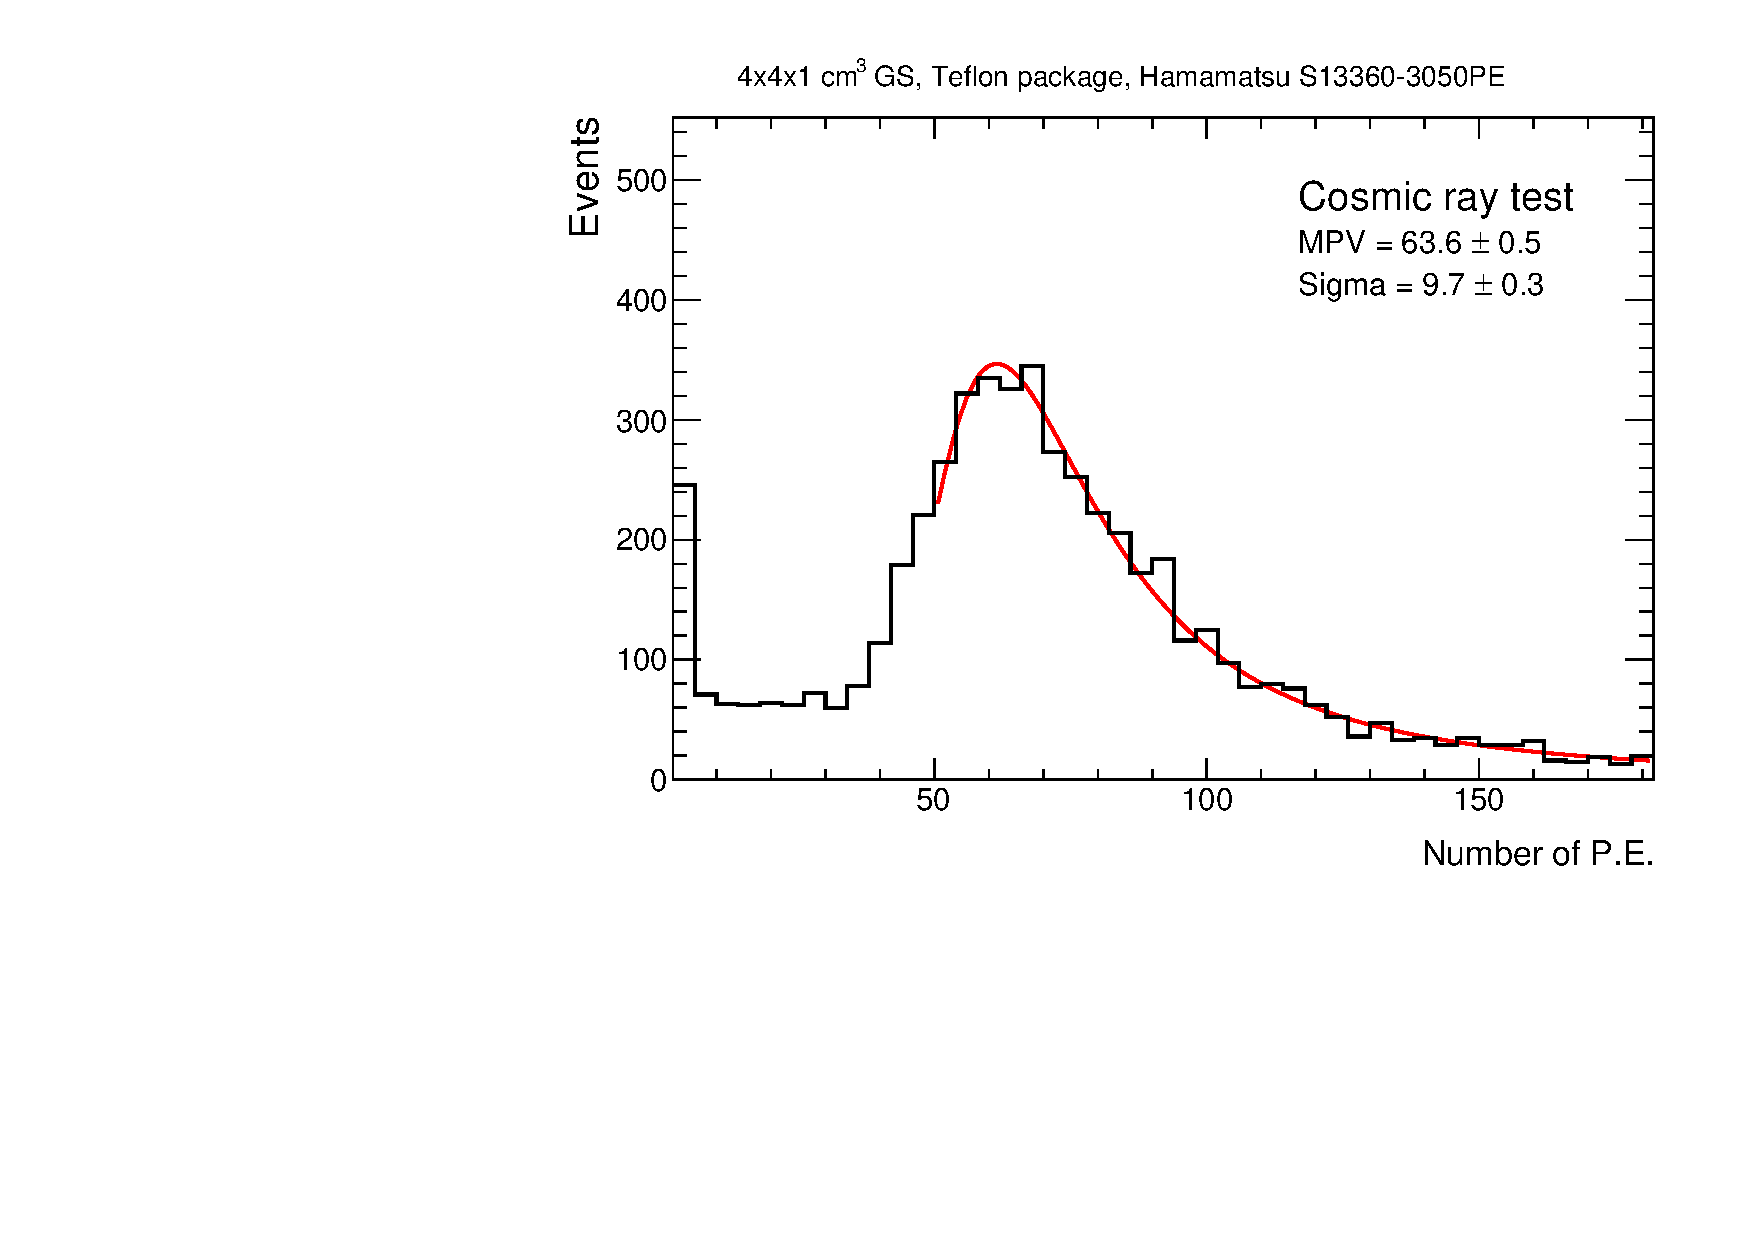
\includegraphics[width=\linewidth]{Cosmic_GSSiPM_SJTU_Teflon.pdf}
  \caption{}
\end{subfigure}

\vspace{0.3cm}

\begin{subfigure}{0.49\textwidth}
  \centering
  \includegraphics[width=\linewidth]{KEK_BeamTest_Electron.png}
  \caption{}
\end{subfigure}
\caption{Single-cell measurement results (\cellsize GS with SiPM
readout).
(a)~ADC spectrum with $^{137}$Cs source (HPK~S14160-3050HS).
(b)~Cosmic-ray test (HPK~S13360-3050PE): $63.6\pm0.5$~\peMIP.
(c)~Response to \SI{5}{GeV} electrons at KEK (NDL~EQR20-11-3030):
Landau-fit MPV $157.6\pm2.9$~\peMIP.}
\label{fig:SiPM_Celltest}
\end{figure}

\paragraph{Interpretation.}
The three probes are complementary rather than directly comparable.
The cosmic-ray muon provides the practical MIP-scale reference
(${\sim}\SI{7.7}{MeV}$ ionisation deposit in \SI{10}{mm} of GFO),
and it is this 64~\peMIP value that enters the baseline digitisation
model (Section~\ref{sec:simperf}).
The \SI{5}{GeV} electron is well above the GFO critical energy
($E_{c}\sim\SI{10}{MeV}$), so it deposits energy through an
electromagnetic shower whose local energy density exceeds that of a
MIP; the resulting 158~\peMIP is therefore higher than the
cosmic-ray value and is not a MIP signal.
The $^{137}$Cs result provides a low-energy check scaled by MIP
equivalence, which is also above the cosmic value.
Taken together the three probes consistently show that the GS cell
plus SiPM provides a signal amplitude well above the threshold
required by the SiPM DCR of Section~\ref{subsec:sipm}, establishing
the practical feasibility of the baseline active unit.
The residual discrepancy with the Geant4 optical simulation
(${\sim}\SI{42}{\peMIP}$) is discussed in
Section~\ref{subsec:optsim}.

%% --------------------------------------------------------------------
\subsection{Reproducibility and quality control}
\label{subsec:qc}
%% --------------------------------------------------------------------

Reproducible tile production is integral to the baseline concept,
because more than five million cells must deliver sufficiently uniform
light yield for PFA reconstruction.
To date approximately 290 tiles of \cellsize have been produced;
about 60\% of them meet the target intrinsic light yield of
\SI{1000}{\phMeV}.
The remaining tile-to-tile variation must be addressed through
two complementary channels: production-side optimisation aiming at a
higher fraction of tiles passing the target, and detector-side
calibration (Section~\ref{subsec:calibration}) that corrects residual
variations through MIP inter-calibration and LED monitoring.
An automated batch-testing platform is being developed to measure
light-yield uniformity, attenuation-length consistency, and
dimensional tolerances across large production batches, and a
production run of approximately \num{10000} tiles is planned to equip
the full-size prototype.
Mass-production optimisation of GFO tile yield and uniformity is
therefore recognised as one of the baseline's open engineering
items.

%% ====================================================================
\section{Simulation framework and projected detector performance}
\label{sec:simperf}
%% ====================================================================

The projected performance of the baseline detector is obtained from
full Geant4 digitisation-based simulation of the baseline geometry
within the CEPCSW framework.
These results are type-B evidence in the classification of
Section~\ref{subsec:why-baseline}: they establish that the baseline
configuration is consistent with the CEPC performance goals under the
current modelling assumptions, before full prototype beam validation.

%% --------------------------------------------------------------------
\subsection{Simulation setup and digitisation assumptions}
\label{subsec:simsetup}
%% --------------------------------------------------------------------

The simulation is performed with Geant4 within the CEPCSW
framework~\cite{CEPCStudyGroup:2018ghi}.
For single-hadron studies all inner sub-detectors are removed so that
the intrinsic GS-HCAL response is isolated; for physics-benchmark
studies the full reference-detector setup is used.
The digitisation model implements the following current modelling
assumptions:

\begin{itemize}
\item \textbf{Birks' constant:} a preliminary value
  $k_{B}=\SI{0.01}{cm/MeV}$, pending a dedicated heavy-ion
  measurement.
\item \textbf{Intrinsic light yield:} \SI{1500}{\phMeV}, giving a
  detected effective single-cell output of $\geq60$~\peMIP.
\item \textbf{Light attenuation length:} \SI{6}{cm}, taken from the
  current transmittance measurement.
\item \textbf{Readout threshold:} \SI{0.1}{MIP}, selected from a
  dedicated scan of its impact on the energy resolution.
\item \textbf{SiPM response and electronics effects:} included with
  the candidate SiPM parameters of Table~\ref{tab:SiPM-tab1}.
\end{itemize}

These are \emph{current modelling assumptions}: they are grounded in
measurements, but a subset of them (notably the Birks constant and
the optical-simulation light yield) is known to require further
tuning, and full experimental closure of the simulation chain is one
of the objectives of the prototype beam-test programme.

%% --------------------------------------------------------------------
\subsection{Single-hadron energy response}
\label{subsec:hadronres}
%% --------------------------------------------------------------------

The single-hadron energy resolution of the GS-HCAL is parametrised as
\begin{equation}
\label{eq:eres}
\frac{\sigma_{E}}{E} = \frac{a}{\sqrt{E}} \oplus b,
\end{equation}
where $a$ is the stochastic term and $b$ the constant term.
With the present digitisation model, and before full prototype beam
validation, the baseline detector configuration predicts
\begin{equation}
\frac{\sigma_{E}}{E} = \frac{29.8\%}{\sqrt{E\,[\text{GeV}]}}
\oplus 6.5\%,
\end{equation}
with energy non-linearity within 2\% (Figure~\ref{fig:Eres_HCAL_final};
\texttt{QGSP\_BERT} hadronic physics list).
The stochastic term is substantially below that of conventional
sampling HCALs (${\sim}60\%/\sqrt{E}\oplus3\%$), reflecting the high
active-medium density of the baseline.
The constant term is larger than the final CEPC target and is
dominated by longitudinal leakage in the $6\,\lambdaI$ design; this is
analysed in Section~\ref{subsec:constterm}.

\begin{figure}[htbp]
\centering
\begin{subfigure}{0.45\linewidth}
  \centering
  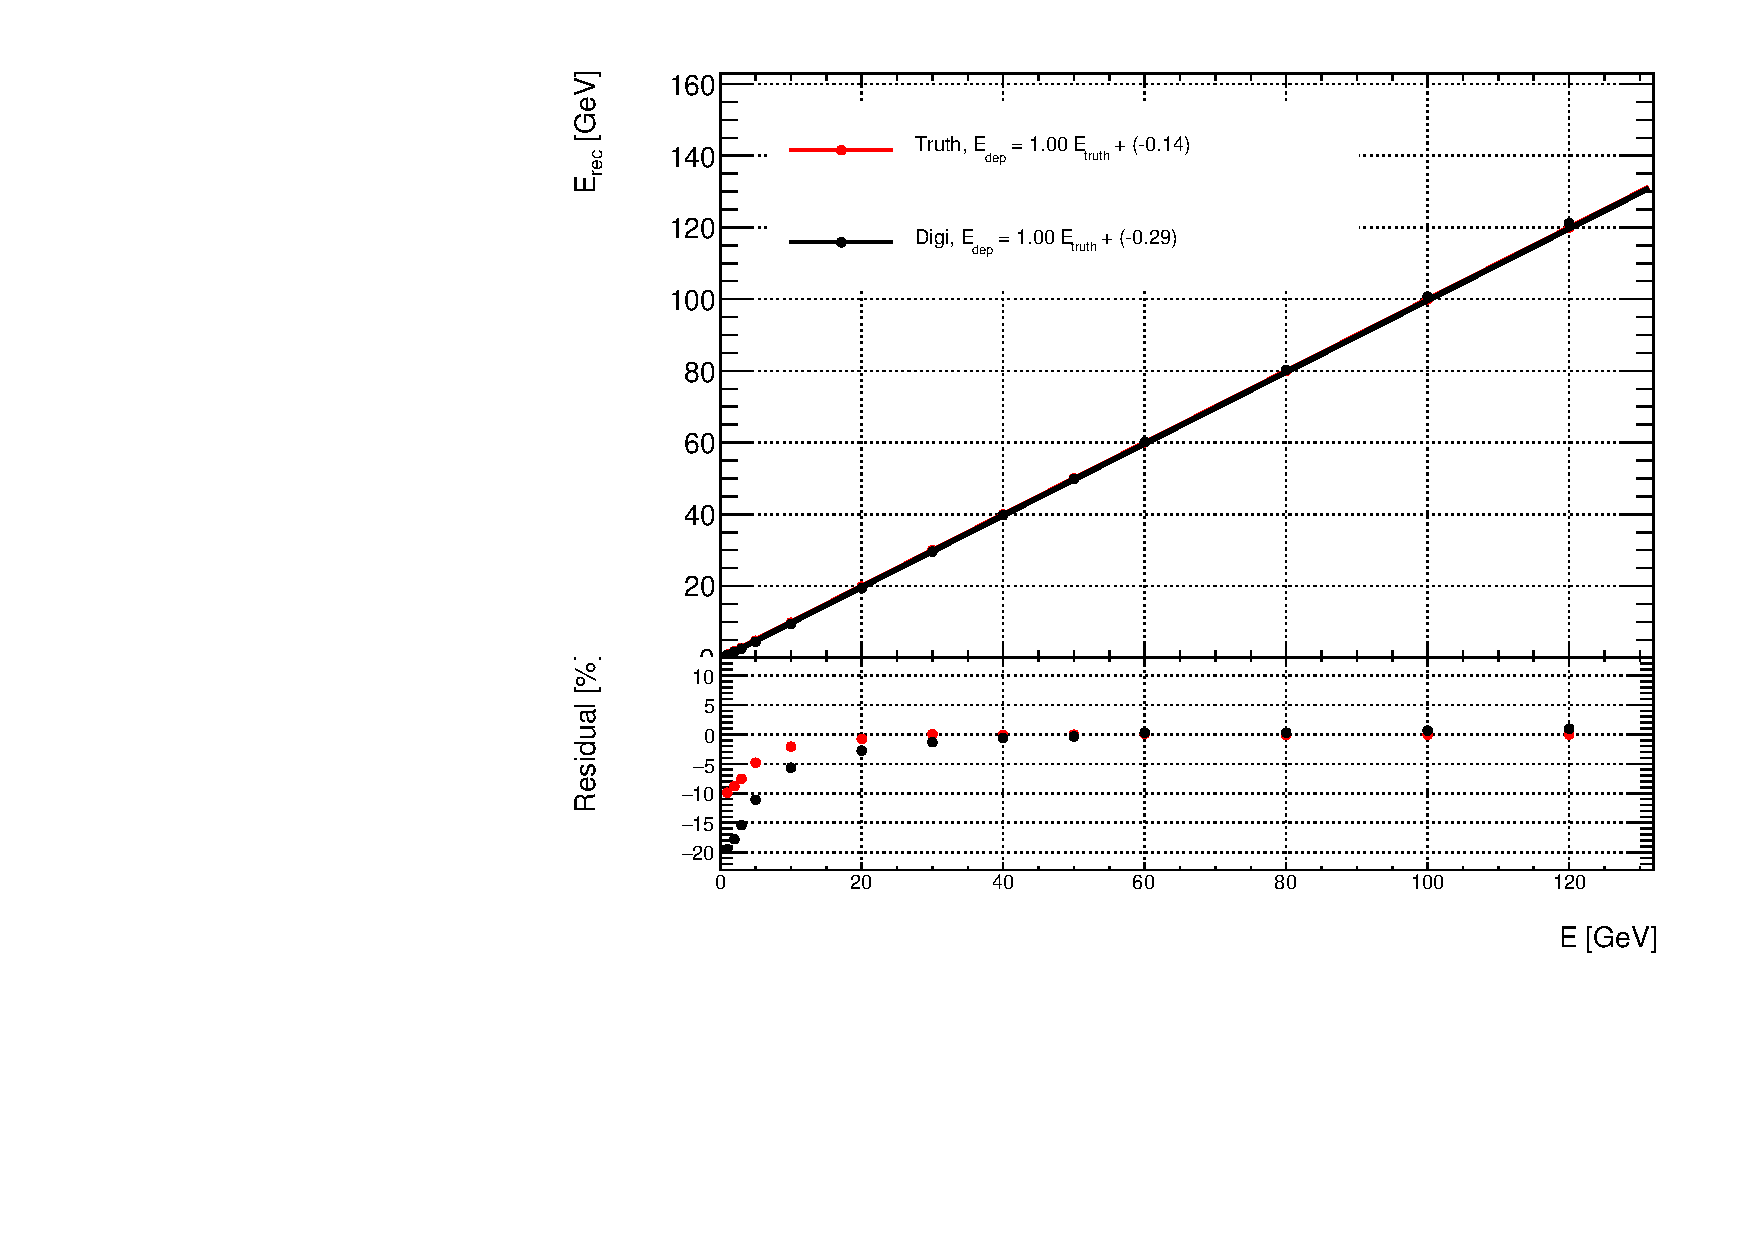
\includegraphics[width=\linewidth]{Elin_digi.pdf}
  \caption{}
\end{subfigure}\hfill
\begin{subfigure}{0.45\linewidth}
  \centering
  \includegraphics[width=\linewidth]{Eres_digi.pdf}
  \caption{}
\end{subfigure}
\caption{(a)~Energy linearity and (b)~energy resolution of the
baseline GS-HCAL from the full digitisation model.}
\label{fig:Eres_HCAL_final}
\end{figure}

In the CEPC collision environment
(Figure~\ref{fig:Ehad_CEPC}), more than 98\% of hadronic final-state
objects have energies below \SI{60}{GeV}, which is precisely the
regime in which the GS-HCAL stochastic term dominates and the
predicted resolution is best.

\begin{figure}[htbp]
\centering
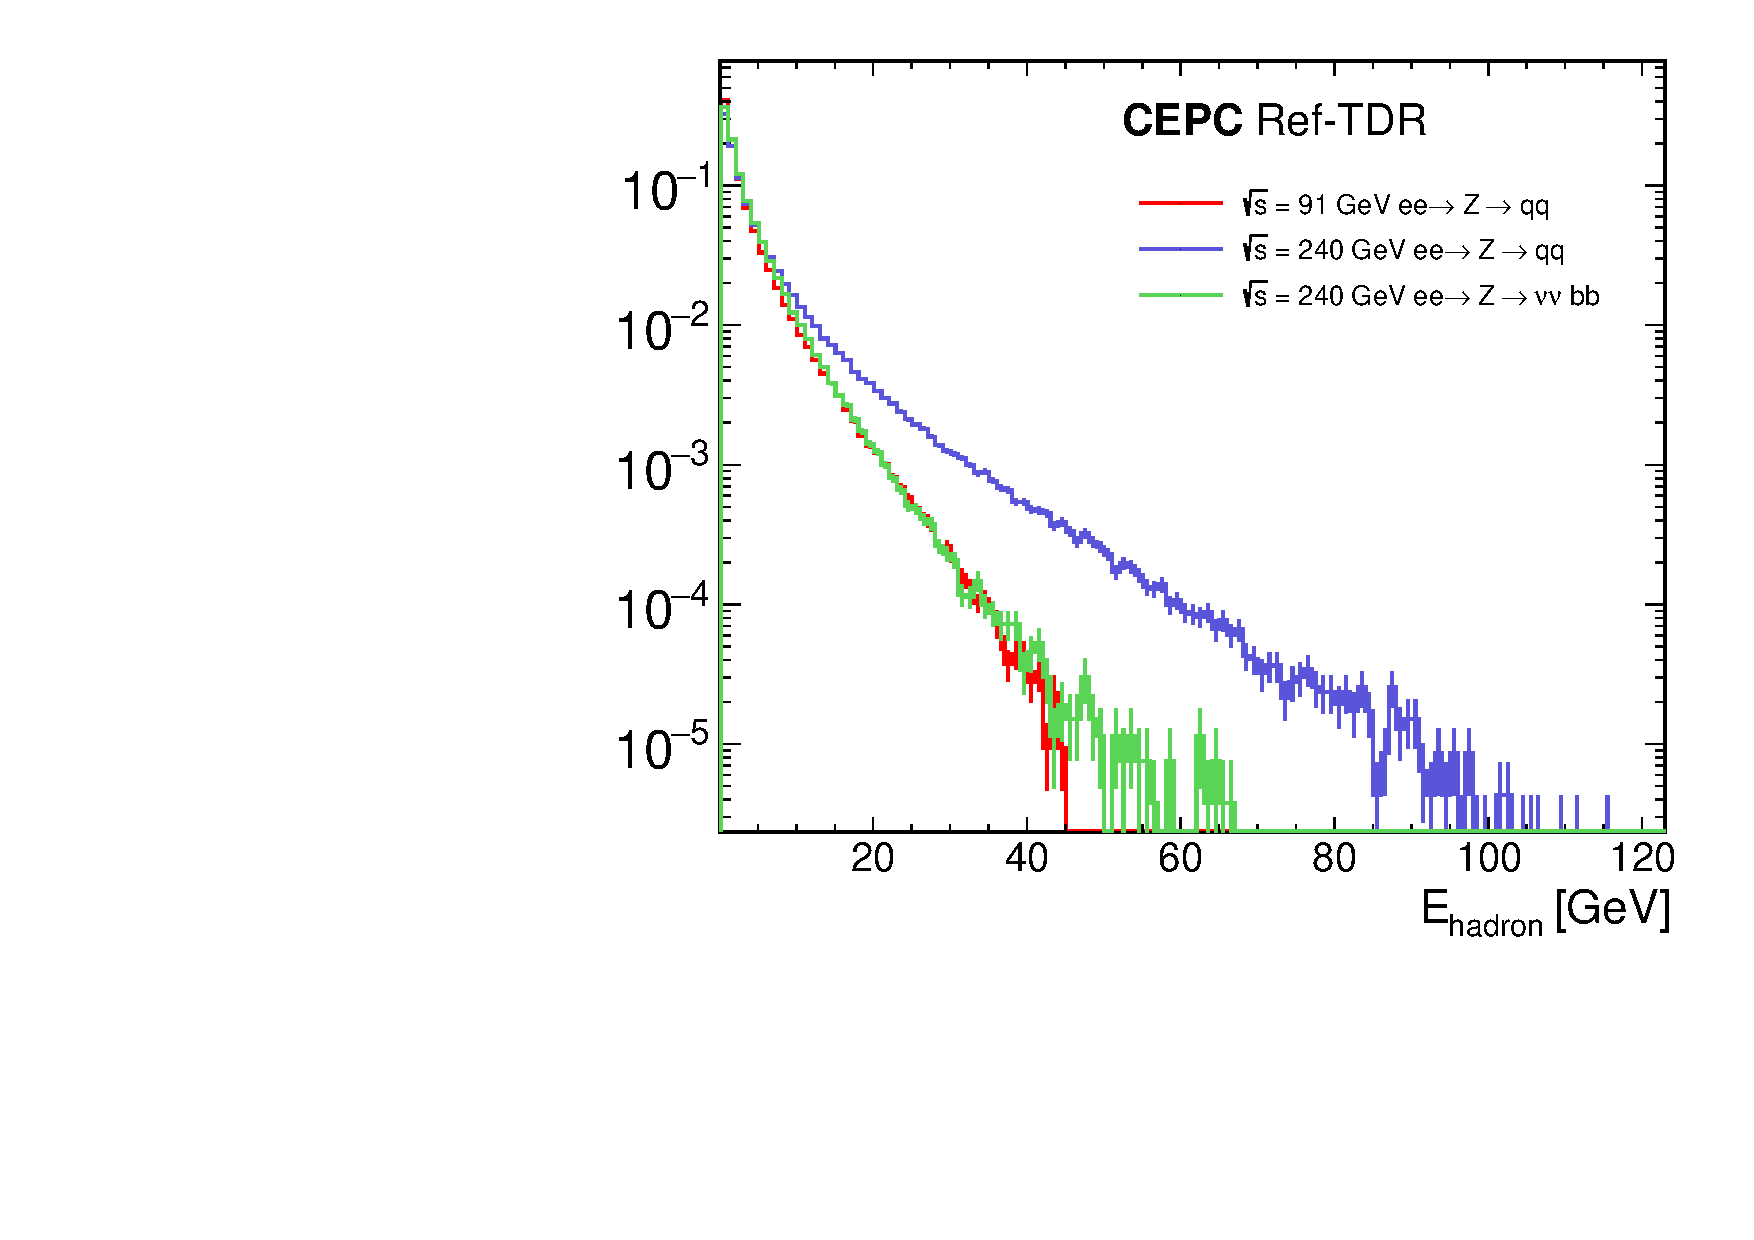
\includegraphics[width=0.50\linewidth]{Ehadrons.pdf}
\caption{Energy distribution of hadronic final-state objects in the
most energetic CEPC $e^{+}e^{-}$ processes.}
\label{fig:Ehad_CEPC}
\end{figure}

%% --------------------------------------------------------------------
\subsection{Sensitivity to key detector parameters}
\label{subsec:sensitivity}
%% --------------------------------------------------------------------

The sensitivity of the predicted single-hadron resolution to the
principal digitisation parameters is shown in
Figure~\ref{fig:Eres_vs_parameters} for
(a)~light output and readout threshold, (b)~attenuation length, and
(c)~Birks' constant.
These scans are not auxiliary: they are evidence that the baseline
parameter choices sit in a stable region of the resolution landscape.
In particular, the achieved cosmic-ray light output of
${\sim}\SI{64}{\peMIP}$ is well inside the saturated region of the
light-output/threshold scan, and the measured attenuation length of
${\sim}\SI{6}{cm}$ is likewise in the plateau of curve~(b).
The Birks-constant dependence quantifies the residual sensitivity
that will be reduced once a dedicated measurement is available.

\begin{figure}[htbp]
\centering
\begin{subfigure}{0.48\linewidth}
  \centering
  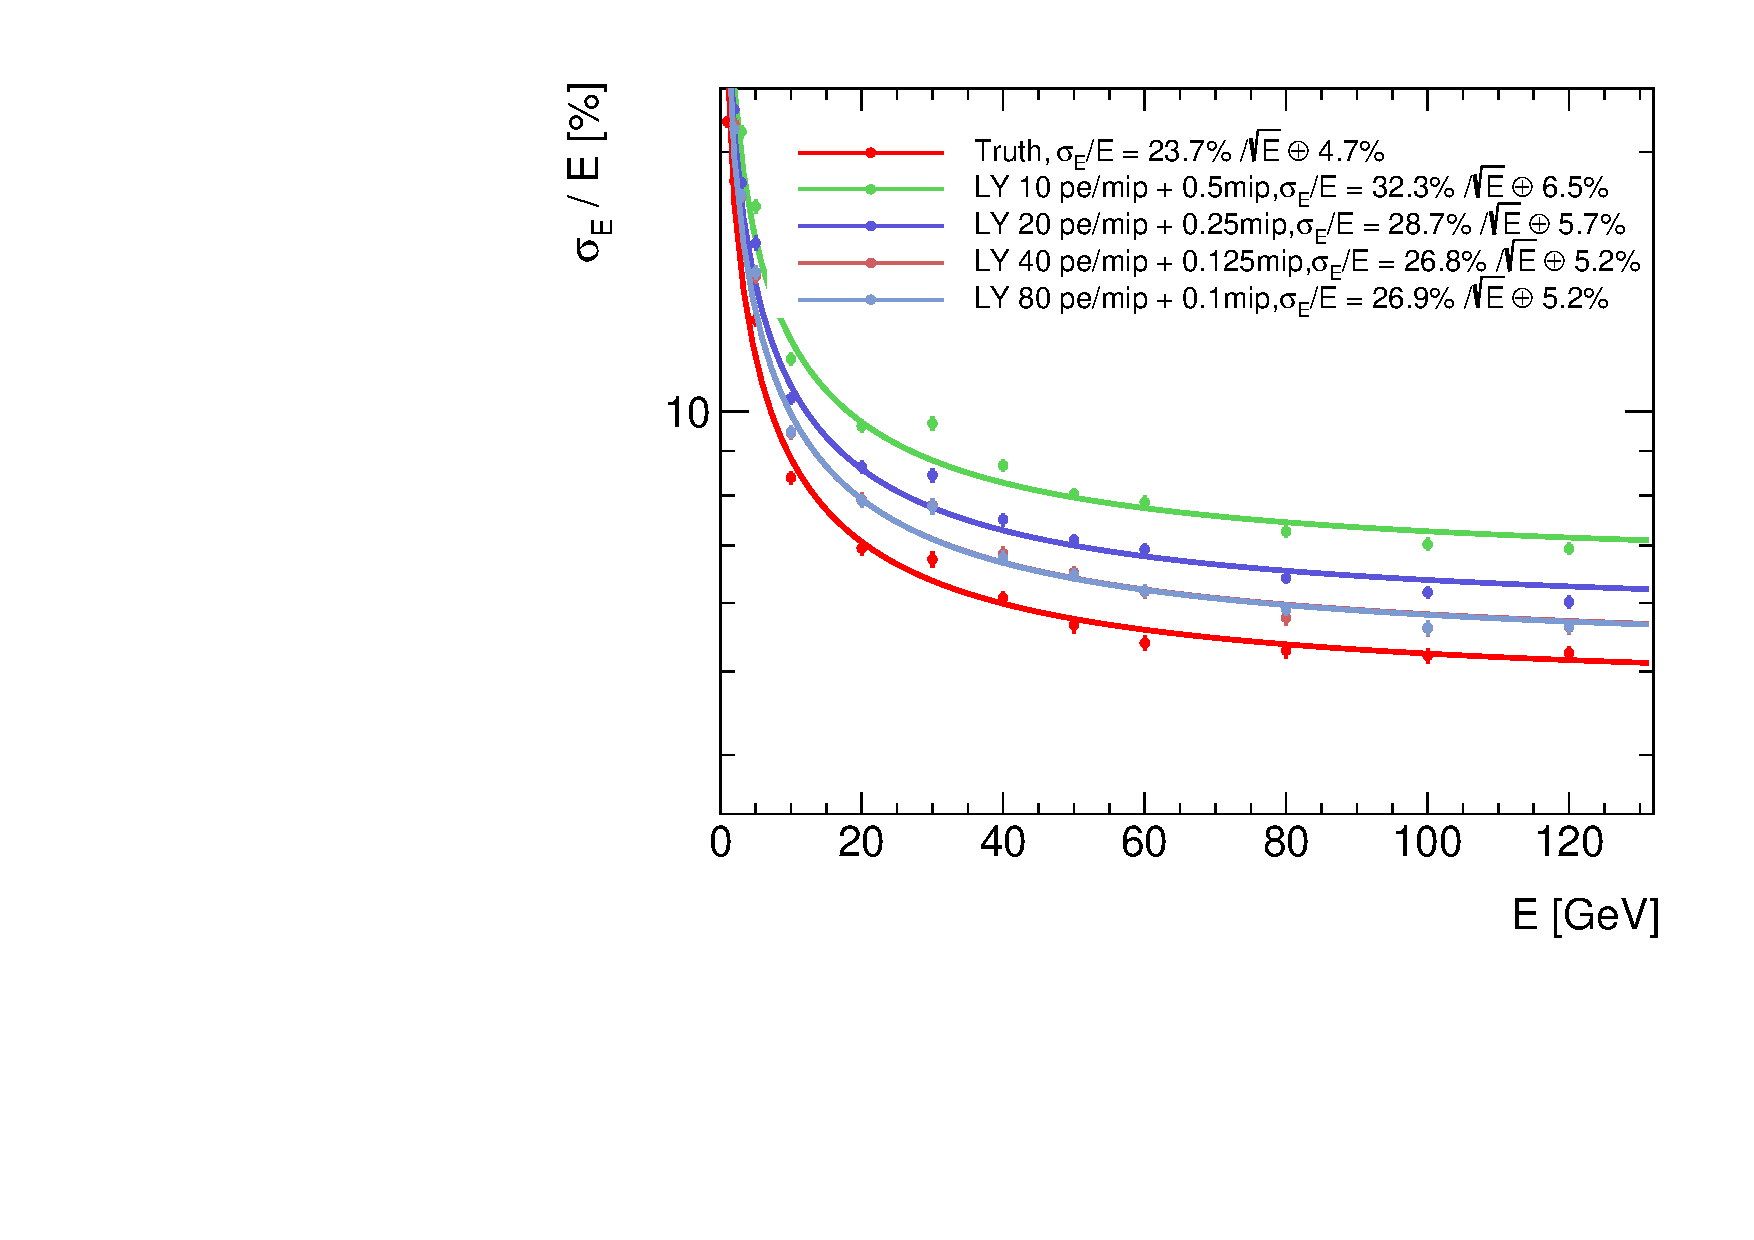
\includegraphics[width=\linewidth]{Eres_LYTh_Log.pdf}
  \caption{}
\end{subfigure}\hfill
\begin{subfigure}{0.48\linewidth}
  \centering
  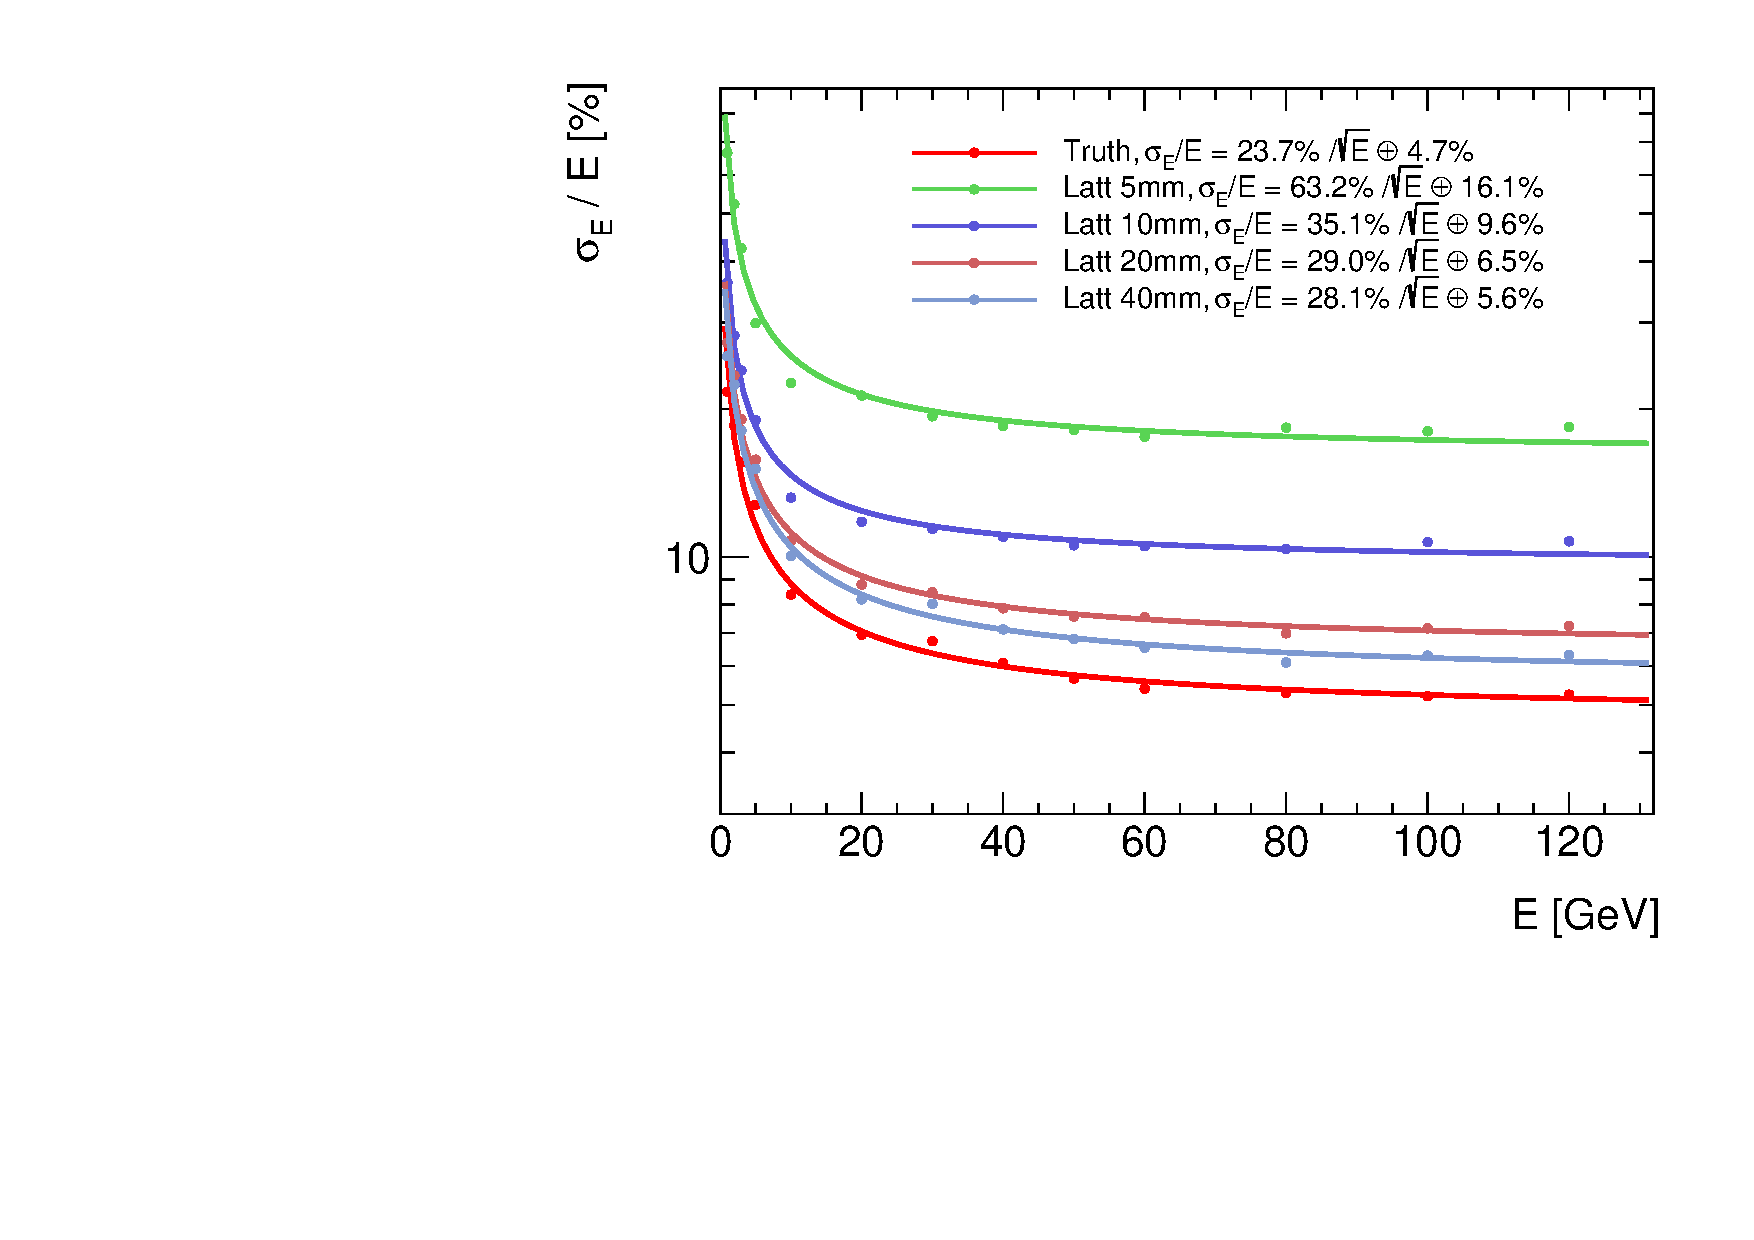
\includegraphics[width=\linewidth]{Eres_Latt_log.pdf}
  \caption{}
\end{subfigure}

\vspace{0.3cm}

\begin{subfigure}{0.48\linewidth}
  \centering
  \includegraphics[width=\linewidth]{ERes_Birks.pdf}
  \caption{}
\end{subfigure}
\caption{Simulated energy resolution as a function of
(a)~light output and readout threshold,
(b)~GS attenuation length, and
(c)~Birks' constant.}
\label{fig:Eres_vs_parameters}
\end{figure}

%% --------------------------------------------------------------------
\subsection{Origin of the constant term}
\label{subsec:constterm}
%% --------------------------------------------------------------------

The 6.5\% constant term obtained in Section~\ref{subsec:hadronres} is
interpreted as being dominated by longitudinal leakage in the
$6\,\lambdaI$ design.
Two independent studies support this interpretation.

First, increasing the standalone HCAL depth from 48~layers
($6\,\lambdaI$) to 80~layers ($10\,\lambdaI$) reduces the constant
term from 4.7\% to 2.9\% (Figure~\ref{fig:depth}), confirming that
leakage is the dominant source.

Second, the upstream environment of the full reference detector is
expected to mitigate this effect.
The BGO ECAL contributes ${\approx}1.2\,\lambdaI$ of upstream
material, causing approximately 70\% of hadrons to initiate showers
before entering the HCAL.
Requiring the first hadronic interaction to occur within the first two
GS-HCAL layers ($0.25\,\lambdaI$) already reduces the constant term to
approximately 3\%, consistent with the PS-HCAL prototype
result~\cite{CALICE:2010fpb,Liu:2025hgf}.

This analysis identifies leakage rather than the intrinsic GS-HCAL
response as the origin of the current constant term; it does not
itself close the constant term, but it shows that the baseline
architecture is compatible with the target 3--4\% BMR.

\begin{figure}[htbp]
\centering
\begin{subfigure}{0.48\textwidth}
  \centering
  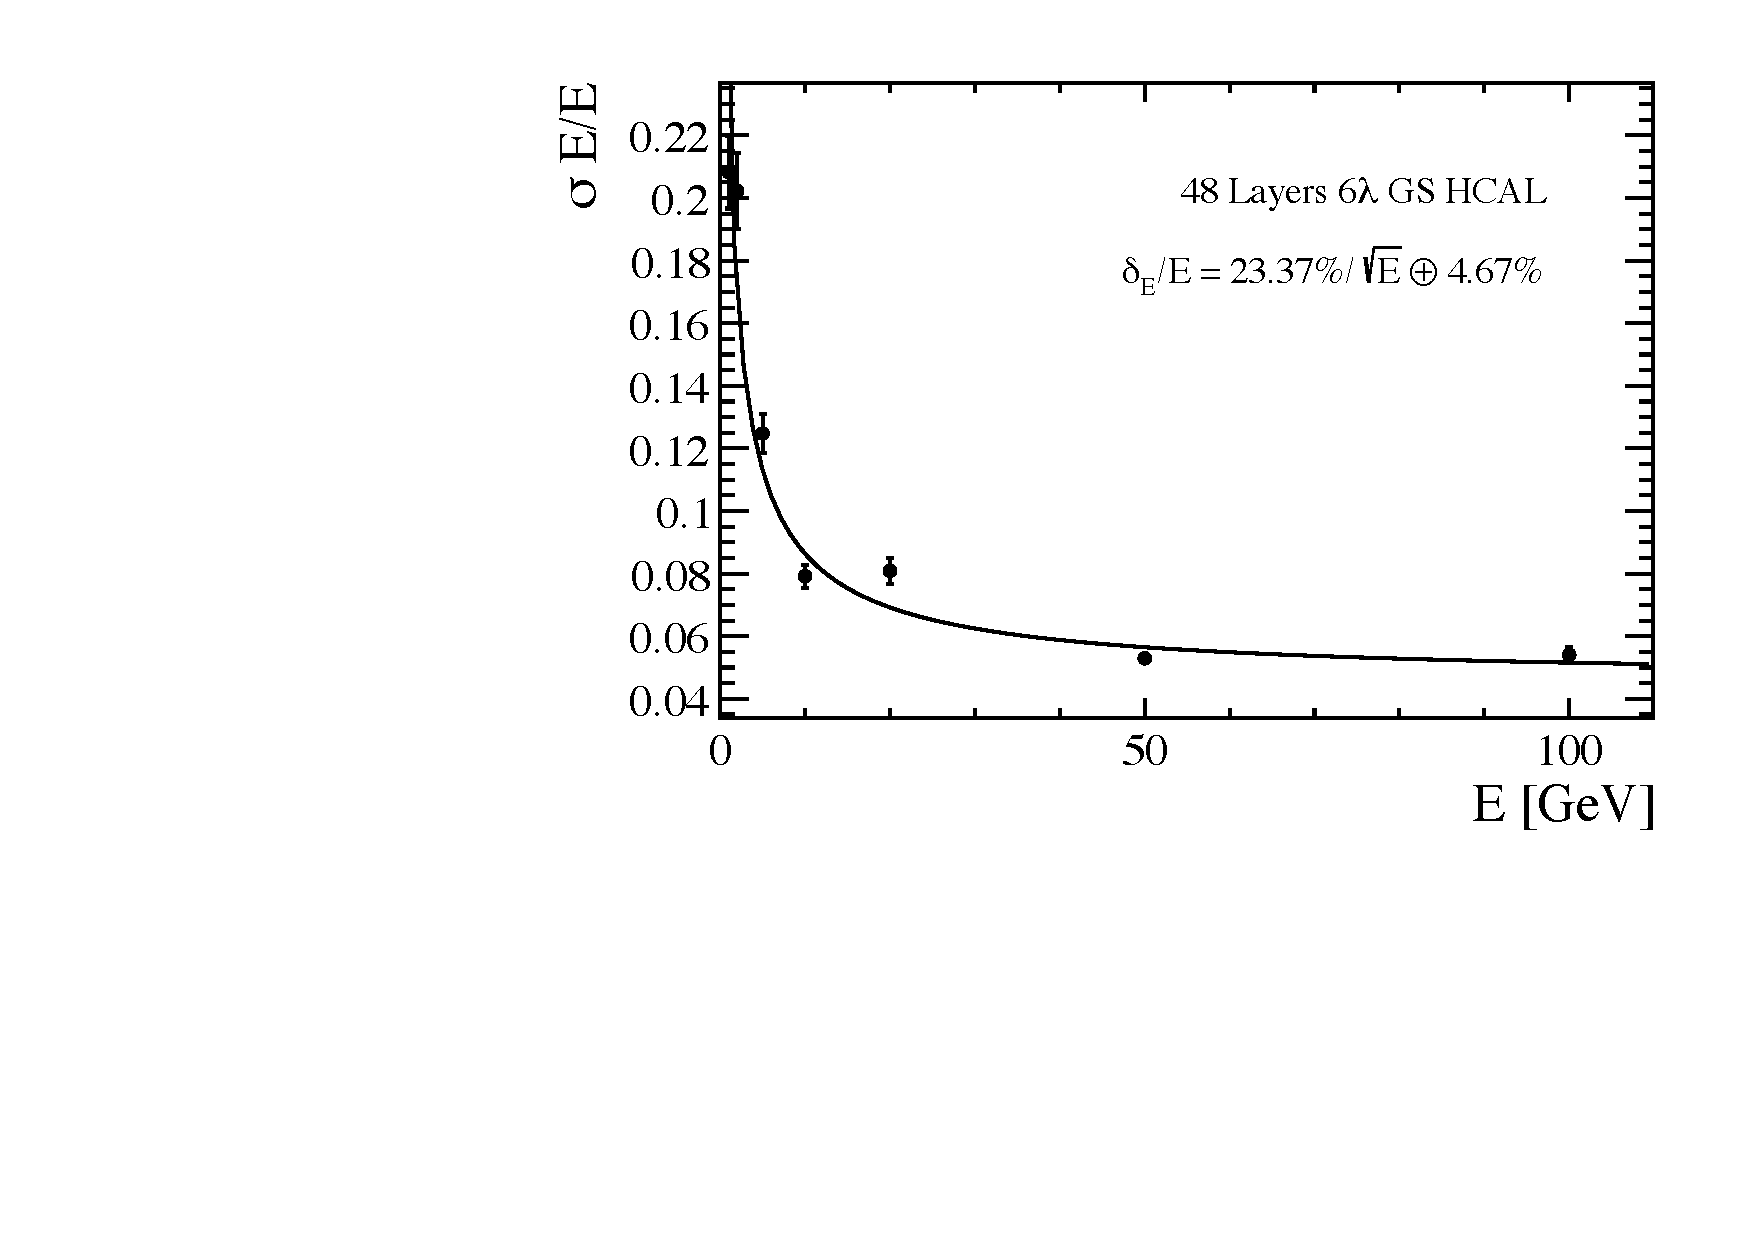
\includegraphics[width=\linewidth]{const_gs_6lambda.pdf}
  \caption{}
\end{subfigure}\hfill
\begin{subfigure}{0.48\textwidth}
  \centering
  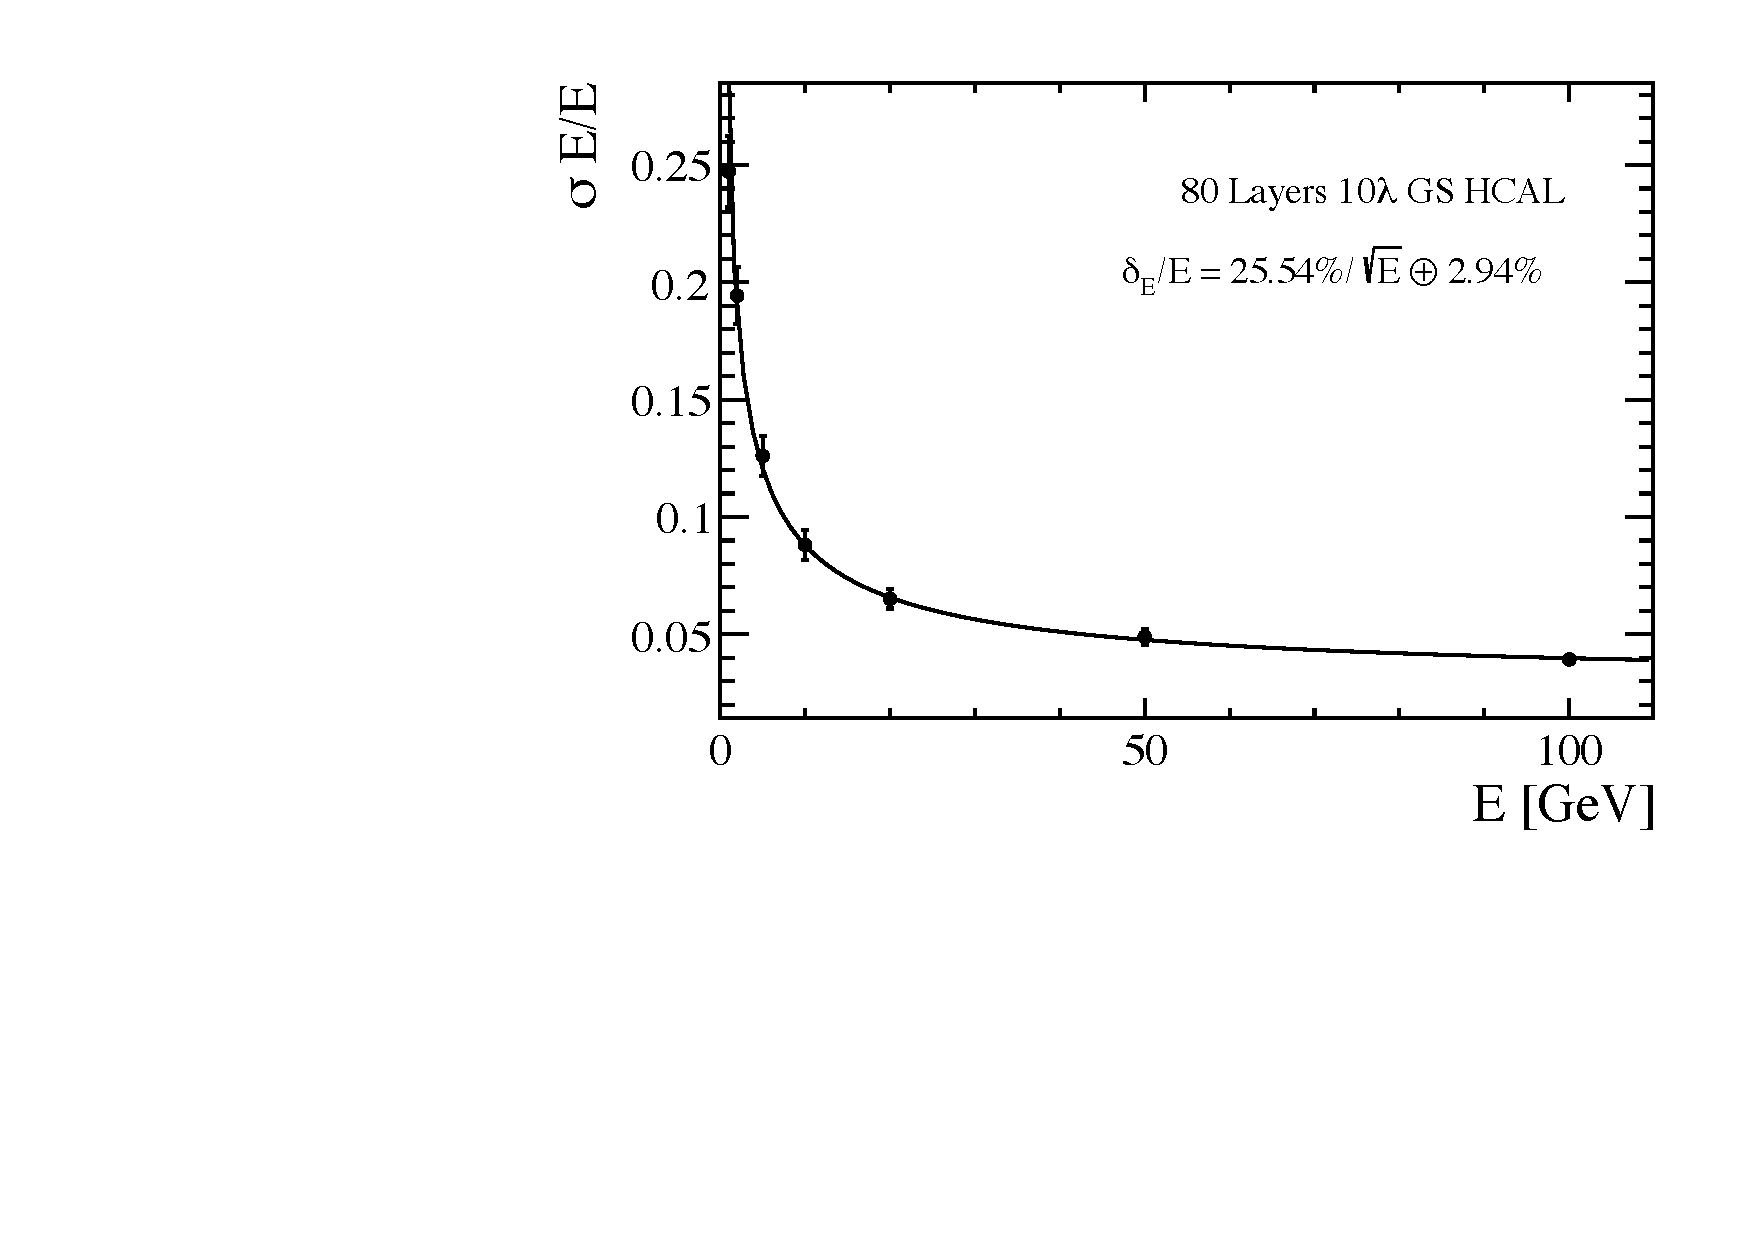
\includegraphics[width=\linewidth]{const_gs_10lambda.pdf}
  \caption{}
\end{subfigure}
\caption{Energy-resolution distributions for two GS-HCAL depths.
(a)~$6\,\lambdaI$ (48~layers): pronounced high-energy tail.
(b)~$10\,\lambdaI$ (80~layers): constant term reduced from 4.7\%
to 2.9\%.}
\label{fig:depth}
\end{figure}

%% --------------------------------------------------------------------
\subsection{Electron--hadron response}
\label{subsec:eresponse}
%% --------------------------------------------------------------------

The baseline calorimeter response to electrons and to different
hadron species is studied with full Geant4 simulation of the
standalone GS-HCAL\@.
Fitting $E_{\mathrm{true}}=C\times S_{\mathrm{HCAL}}$ separately for
each species gives the calibration slopes of
Table~\ref{tab:eoverh_hcal}.
The empirical hadron-to-electron response ratio
$C_{\mathrm{hadron}}/C_{e}$ of 1.09--1.14 is consistent with a
non-compensating sampling calorimeter~\cite{Akchurin:2012zz}.
The empirical ratio must be distinguished from the intrinsic
compensation ratio $e/h$ of the shower physics, which is the actual
figure of merit for the constant term; the intrinsic $e/h$ has not
yet been extracted, and its extraction through shower-component
decomposition is part of the open-item list of
Section~\ref{sec:discussion}.
Software-compensation and energy-weighting techniques
exploiting this intrinsic $e/h$ are expected to reduce the constant
term below~3\%.

\begin{table}[htbp]
\centering
\caption{Calibration slopes $C$ and electron--hadron response ratios
$C_{\mathrm{hadron}}/C_{e}$ for the baseline GS-HCAL\@.}
\label{tab:eoverh_hcal}
\begin{tabular}{lcc}
\toprule
Particle & $C$ (slope) & $C_{\mathrm{hadron}}/C_{e}$ \\
\midrule
Electron  & $2.94\pm0.01$ & ---            \\
$\pi^{-}$ & $3.20\pm0.05$ & $1.09\pm0.02$ \\
$K^{+}$   & $3.28\pm0.05$ & $1.12\pm0.02$ \\
Neutron   & $3.35\pm0.07$ & $1.14\pm0.02$ \\
Proton    & $3.36\pm0.07$ & $1.14\pm0.02$ \\
\bottomrule
\end{tabular}
\end{table}

%% --------------------------------------------------------------------
\subsection{Physics benchmark: $H\to gg$}
\label{subsec:physperf}
%% --------------------------------------------------------------------

The physics-benchmark performance of the baseline is evaluated through
PFA reconstruction of $H\to gg$, the most HCAL-sensitive of the
standard Higgs-dijet benchmarks.
Events are generated with \textsc{Whizard}\,v1.9.5~\cite{Kilian:2007gr,
Moretti:2001zz} and propagated through the full reference-detector
simulation with Geant4\,v11.2 in the CEPCSW framework.
Figure~\ref{fig:ch08_BMR} shows the reconstructed dijet invariant
mass; the fitted Higgs-boson mass is
$126.32\pm0.04$~GeV/$c^{2}$ with
$\sigma(m_{jj})=4.90\pm0.04$~GeV/$c^{2}$, corresponding to a boson
mass resolution (BMR) of 3.88\%, within the CEPC target of 3--4\%.

This result is detector-level strong evidence that the baseline
concept is compatible with the CEPC physics goals, but it is
simulation-based and does not replace prototype beam validation.

\begin{figure}[htbp]
\centering
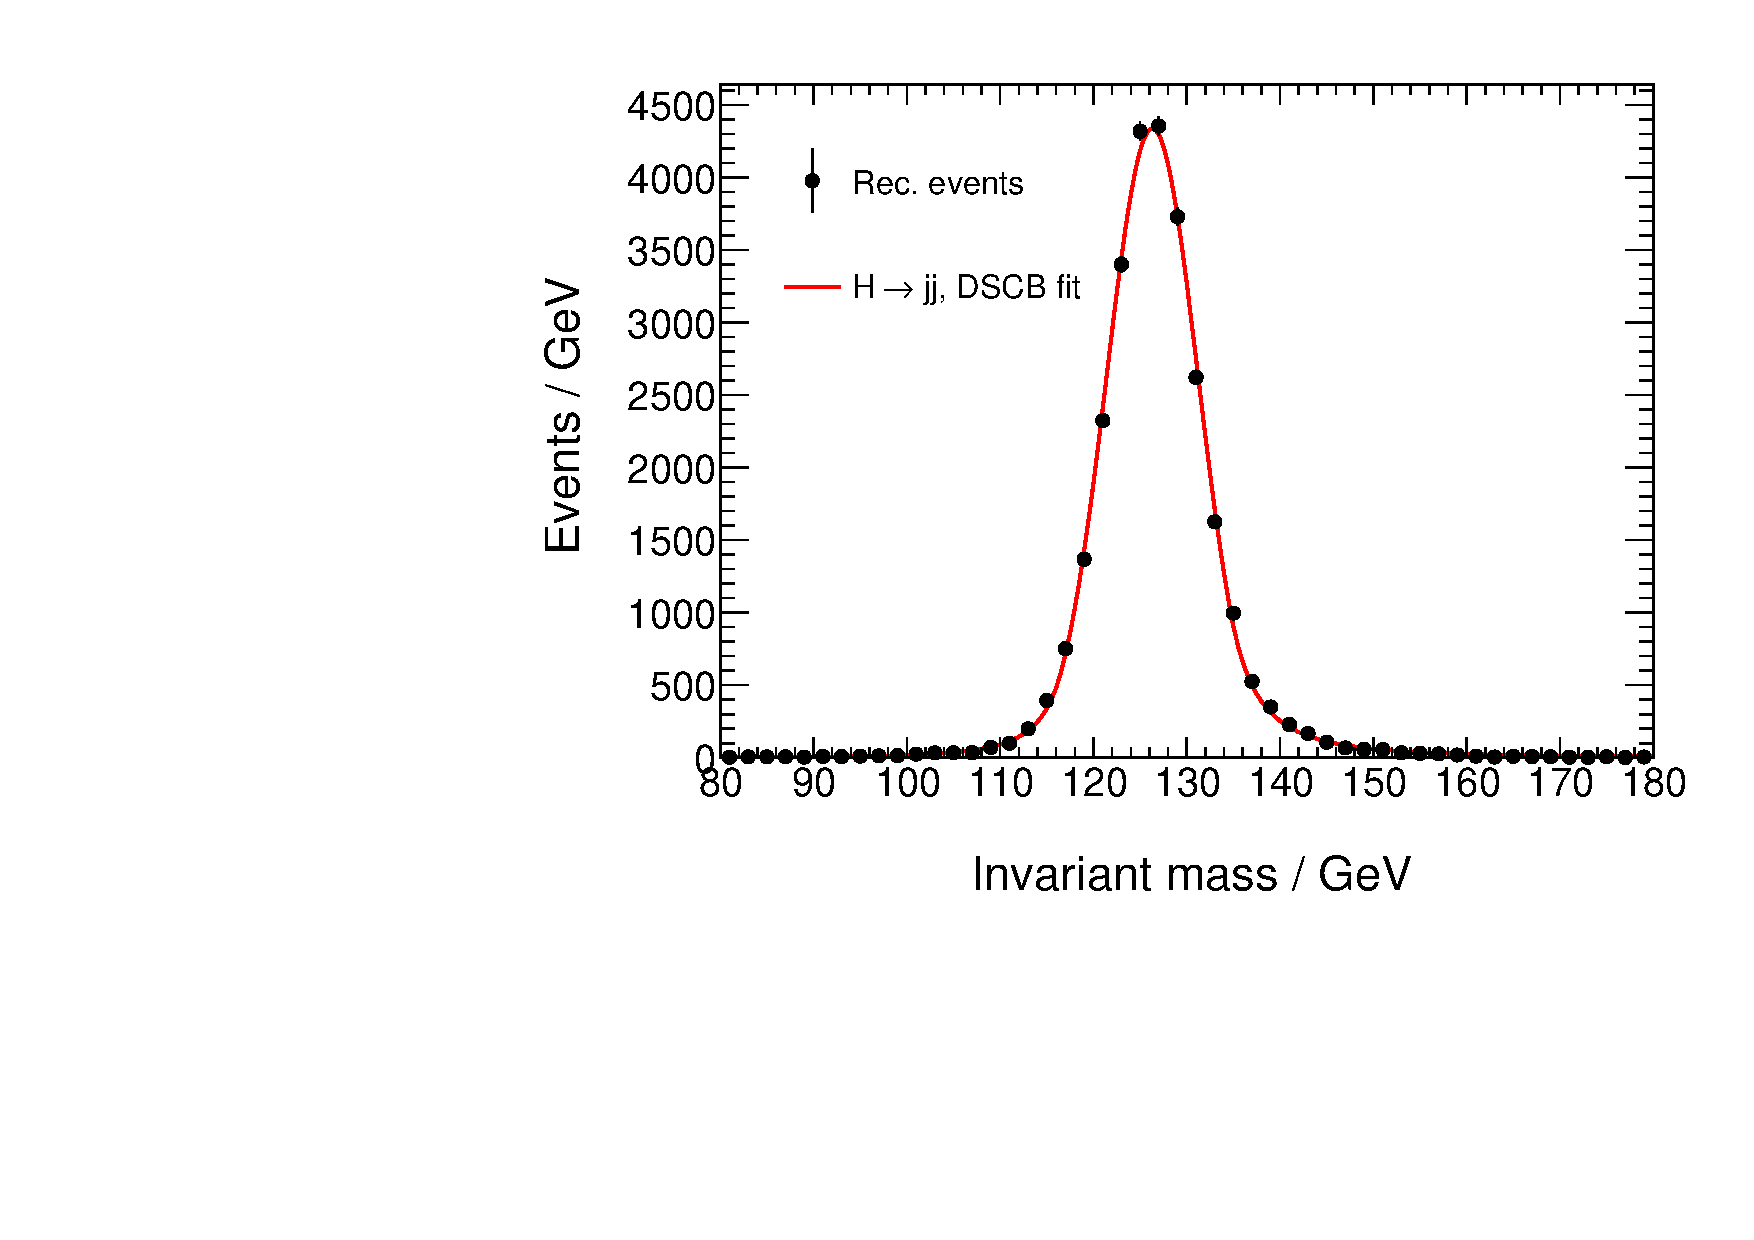
\includegraphics[width=0.60\linewidth]{Fig8.9_BMR.pdf}
\caption{Reconstructed dijet invariant mass for $H\to gg$ with the
baseline GS-HCAL\@.
Fitted mass: $126.32\pm0.04$~GeV/$c^{2}$;
$\sigma(m_{jj})=4.90\pm0.04$~GeV/$c^{2}$; BMR~=~3.88\%.}
\label{fig:ch08_BMR}
\end{figure}

%% ====================================================================
\section{Mechanical feasibility, calibration strategy, and prototype
validation}
\label{sec:feasibility}
%% ====================================================================

Establishing the technical basis of the baseline requires not only
material and simulation evidence but also demonstrated detector-scale
mechanical viability, a defined calibration architecture, and a
concrete prototype beam-test plan.
These three aspects are presented together because they jointly
determine whether the baseline can be realised at full scale.

%% --------------------------------------------------------------------
\subsection{Mechanical feasibility at detector scale}
\label{subsec:mechanics}
%% --------------------------------------------------------------------

Finite-element analysis of the full barrel+endcap structure supports
the detector-scale mechanical viability of the baseline concept.
The critical load is the \SI{135}{t} BGO ECAL supported by the
barrel while the layer-to-layer alignment required by PFA is
preserved.
Figure~\ref{fig:deformation_barrel} shows the deformation distribution
with and without ECAL loading.

\begin{figure}[htbp]
\centering
\begin{subfigure}{0.80\linewidth}
  \centering
  \includegraphics[width=\linewidth]{1.7.1.3.3-3.png}
  \caption{}
\end{subfigure}

\vspace{0.3cm}

\begin{subfigure}{0.80\linewidth}
  \centering
  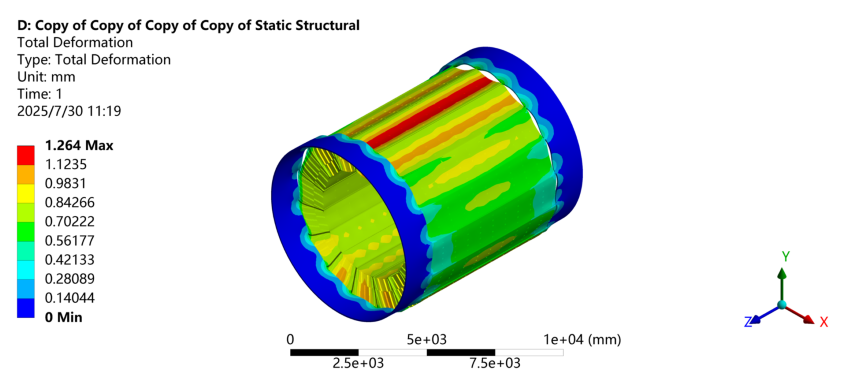
\includegraphics[width=\linewidth]{1.7.1.3.3-2.png}
  \caption{}
\end{subfigure}
\caption{Deformation distribution of the GS-HCAL barrel (a)~without
and (b)~with ECAL loading.}
\label{fig:deformation_barrel}
\end{figure}

During assembly the maximum deformation remains below \SI{0.66}{mm}
and the localised stress below \SI{190}{MPa}, well under the yield
strength.
Under the full ECAL load, peak stresses reach \SI{371}{MPa} at
specific connection points; these critical areas employ titanium-alloy
(TC4) components with safety factors above~2.2, while the bulk of the
structure is stainless steel.
Layer-to-layer deformation differences remain below \SI{0.2}{mm}
(within the \SI{2.4}{mm} gasket range), intra-layer deformations are
below \SI{0.5}{mm} inducing only \SI{20}{MPa} stress in the GS cells,
and the scintillator boxes withstand \SI{0.5}{mm} bending with a
safety factor above three.
Taken together, these results support the detector-scale mechanical
viability of the baseline concept; they are type-B evidence on the
engineering side, complementing the simulation-based detector
performance of Section~\ref{sec:simperf}.

%% --------------------------------------------------------------------
\subsection{Calibration strategy as part of the baseline architecture}
\label{subsec:calibration}
%% --------------------------------------------------------------------

Calibration is integral to the baseline concept rather than an
auxiliary activity: with 5.22~million channels and tile-to-tile light
yield variations, no operating point of the detector is reachable
without a well-defined calibration architecture.
The baseline therefore incorporates two complementary calibration
layers, physics-process calibration and hardware calibration.

\paragraph{Physics-process calibration.}
Global calibration exploits MIP signals from
$e^{+}e^{-}\to Z\to\mu^{+}\mu^{-}$ events.
At design luminosity the process rate is \SI{584}{Hz}, corresponding
to approximately 47~events per hour within a $\Delta\phi\times
\Delta\!\cos\theta=0.018\times0.018$ acceptance window matched to
one central-barrel HCAL cell (Figure~\ref{fig:kinematic_mumu}).
Bi-weekly \SI{16}{h/day} calibration runs accumulate
$4.71\times10^{8}$ di-muon events, yielding ${\sim}1\%$ statistical
precision per cell.
In addition, $e^{+}e^{-}\to Z\to q\bar{q}$ (Figure~\ref{fig:kinematic_zjj})
provides resonant dijets for combined ECAL+HCAL response
calibration through the reconstructed $m_{jj}$, and hadronic $\tau$
decays in $Z\to\tau^{+}\tau^{-}$ provide complementary $E/p$
monitoring over time.

\begin{figure}[htbp]
\centering
\begin{subfigure}{0.32\textwidth}
  \centering
  \includegraphics[width=\linewidth]{Fig8_mumu_cosTheta.pdf}
  \caption{}
\end{subfigure}\hfill
\begin{subfigure}{0.32\textwidth}
  \centering
  \includegraphics[width=\linewidth]{Fig8_mumu_phi.pdf}
  \caption{}
\end{subfigure}\hfill
\begin{subfigure}{0.32\textwidth}
  \centering
  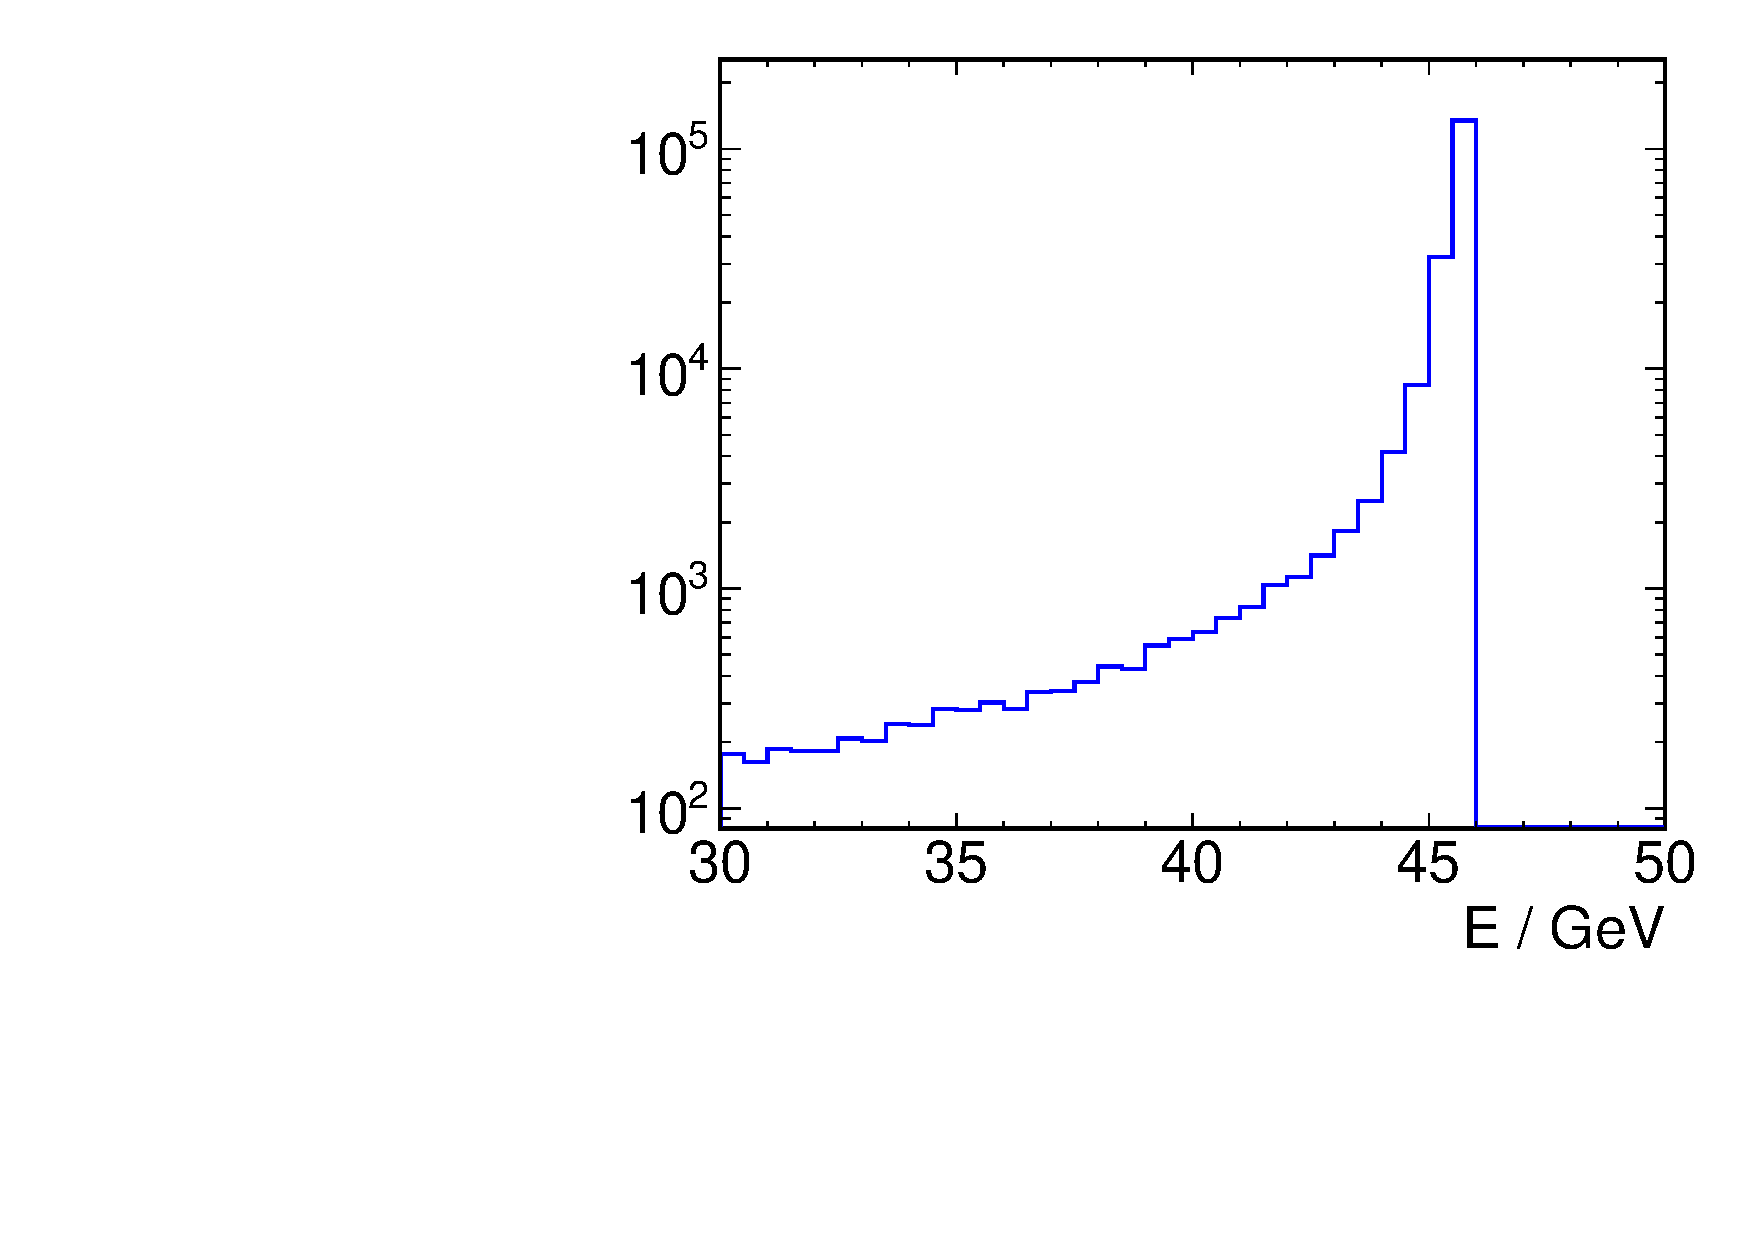
\includegraphics[width=\linewidth]{Fig8_mumu_E.pdf}
  \caption{}
\end{subfigure}
\caption{Generator-level distributions of (a)~$\cos\theta$, (b)~$\phi$,
and (c)~energy of muons in $e^{+}e^{-}\to\mu^{+}\mu^{-}$ at
$\sqrt{s}=\SI{91.2}{GeV}$.}
\label{fig:kinematic_mumu}
\end{figure}

\begin{figure}[htbp]
\centering
\includegraphics[width=0.50\textwidth]{Mjj_eeuu_91.pdf}
\caption{Distribution of dijet invariant mass from $Z\to q\bar{q}$ at
$\sqrt{s}=\SI{91.2}{GeV}$.}
\label{fig:kinematic_zjj}
\end{figure}

\paragraph{Hardware calibration.}
The hardware calibration comprises MIP inter-calibration using cosmic
rays or muon beams, and an online LED-based monitoring system with
optical-fibre distribution to multiple cells
(Figure~\ref{fig:Calibration-2n}).
The LED system continuously tracks pedestals, gain, and response
linearity at the single-cell level.

\begin{figure}[htbp]
\centering
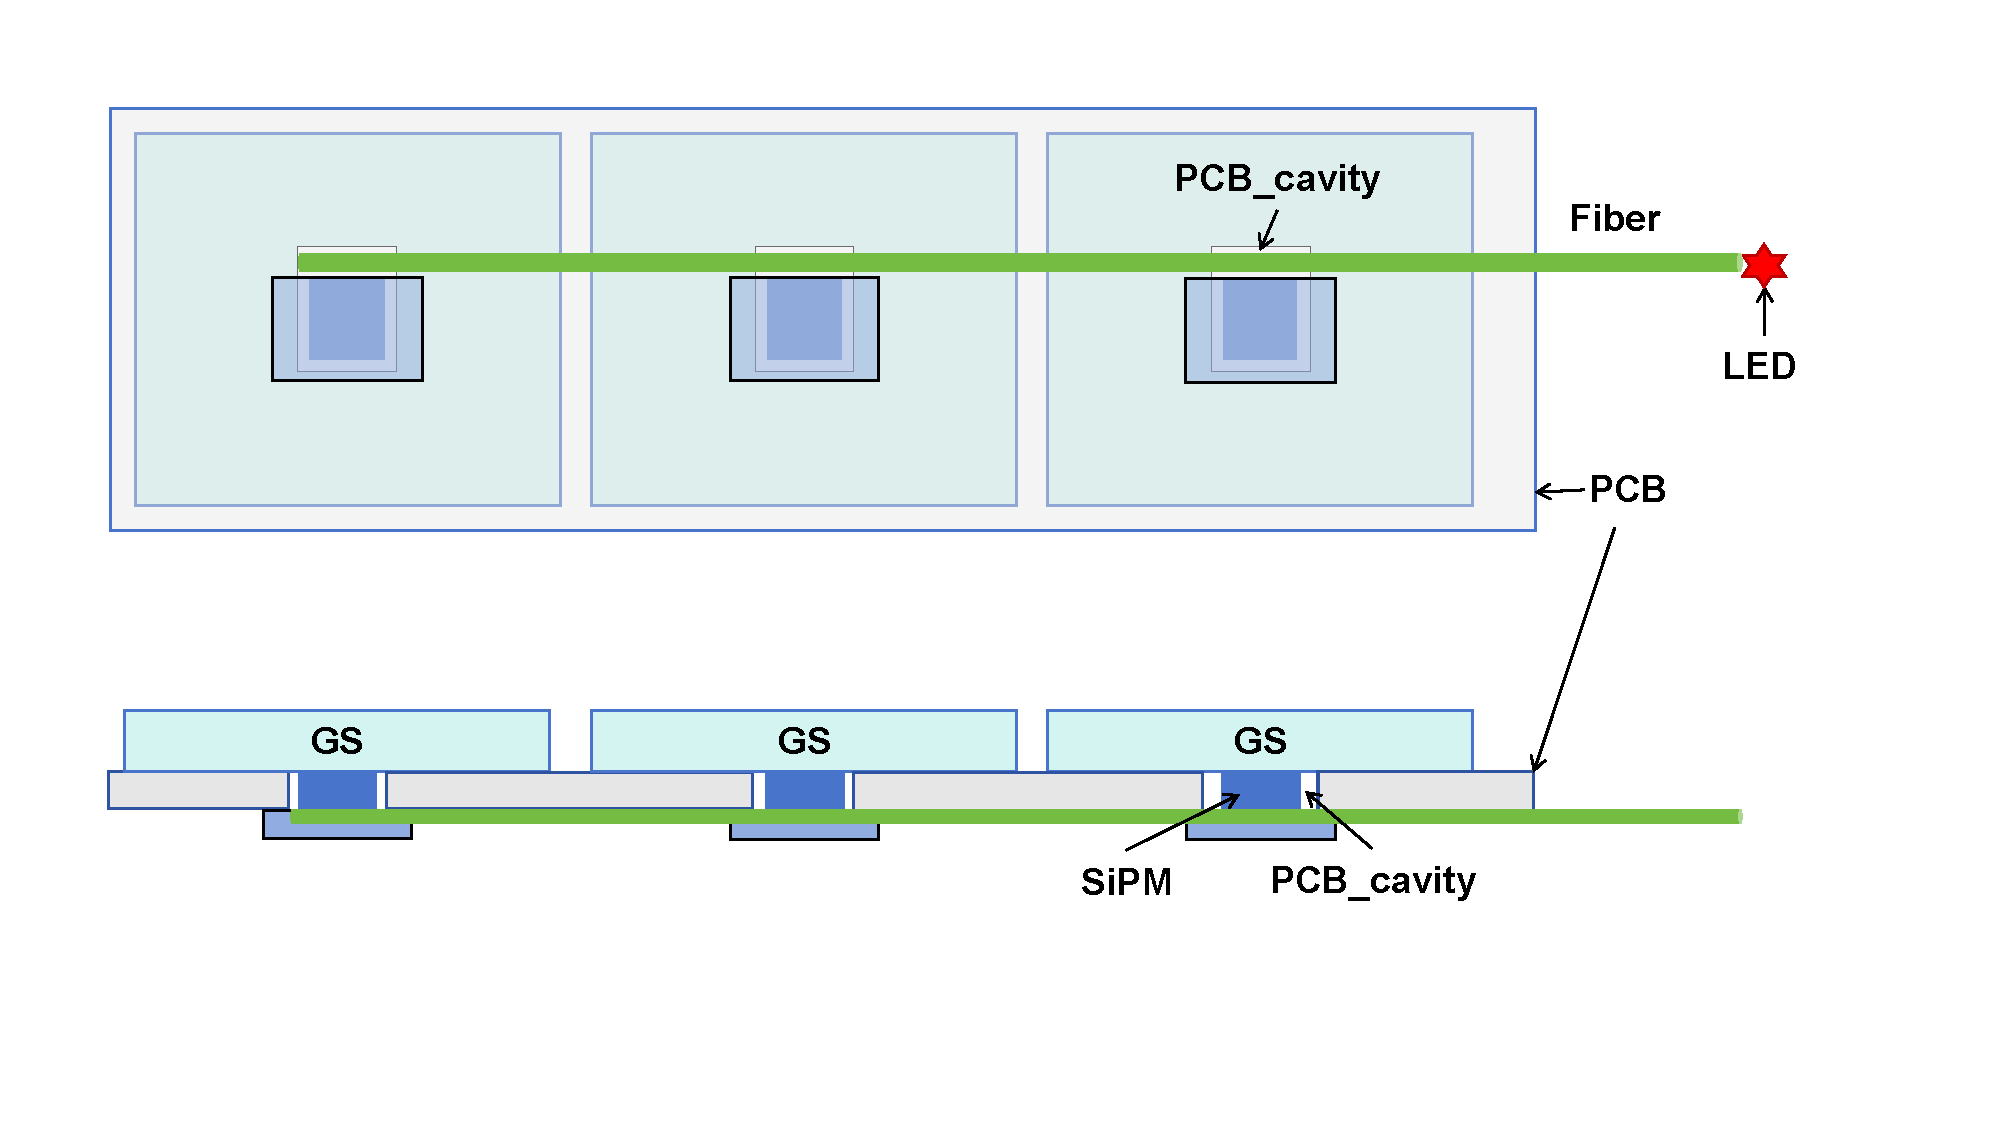
\includegraphics[width=0.68\textwidth]{Calibration-2n.pdf}
\caption{Schematic of the GS-HCAL LED calibration system showing
optical-fibre connections between adjacent cells: top~view~(a) and
side~view~(b).}
\label{fig:Calibration-2n}
\end{figure}

The two layers are complementary: the physics-process layer provides
absolute energy-scale closure in situ, while the hardware layer
provides the fast monitoring loop between physics calibrations.
The baseline design cannot be realised without both, and this is why
they are presented as components of the detector concept rather than
as post-hoc add-ons.

%% --------------------------------------------------------------------
\subsection{Prototype validation strategy}
\label{subsec:prototype}
%% --------------------------------------------------------------------

A GS-HCAL prototype is under construction to provide the validation
path of the baseline detector concept.
The prototype is a steel-scintillator sandwich of
$52.0\times52.0\times130.6$~cm$^{3}$ (${\approx}0.6$~m$^{3}$),
containing 8112~GS cells in 48~layers (${\approx}6\,\lambdaI$).
Each layer is a $13\times13$ array of \cellsize cells, each coupled
to a \sipmsize SiPM, with \SI{9.8}{mm} S304 stainless-steel absorber
plates.

Geant4 simulations with \SI{80}{GeV} $\pi^{-}$ beams show that this
$13\times13\times48$ configuration reaches 95\% energy containment
(Figure~\ref{fig:prototype-sim-energy}), and projects a prototype
single-hadron resolution of ${\sim}45\%/\sqrt{E}\oplus8\%$,
degraded relative to the full detector because of the limited
transverse extent but sufficient to validate the key baseline
technologies and reconstruction algorithms
(Figure~\ref{fig:prototype-sim-resolution}).

\begin{figure}[htbp]
\centering
\includegraphics[width=0.50\linewidth]{Edep_module_80GeV.pdf}
\caption{Simulated deposited energy in prototypes of different lateral
sizes for \SI{80}{GeV} $\pi^{-}$; the $13\times13\times48$
configuration achieves ${\approx}95\%$ containment.}
\label{fig:prototype-sim-energy}
\end{figure}

\begin{figure}[htbp]
\centering
\begin{subfigure}{0.40\textwidth}
  \centering
  \includegraphics[width=\linewidth]{prototype_simulation-13}
  \caption{}
\end{subfigure}\hfill
\begin{subfigure}{0.40\textwidth}
  \centering
  \includegraphics[width=\linewidth]{prototype_simulation-linear.jpg}
  \caption{}
\end{subfigure}
\caption{Simulated (a)~energy resolution and (b)~energy linearity of
the GS-HCAL prototype.}
\label{fig:prototype-sim-resolution}
\end{figure}

The validation proceeds in two stages:
a $3\times3\times7$ mini-prototype tests integration of the GS cell,
SiPM, front-end, and calibration at reduced scale;
the full 8112-channel prototype then exercises the complete baseline
active unit and provides the measured detector response against which
the Geant4 optical model, the Birks constant, the intrinsic $e/h$
extraction, and the constant-term interpretation can be closed.
Together with the measured containment and projected prototype
resolution, this establishes a clear closure path from the
current evidence to a fully validated baseline.

%% ====================================================================
\section{Discussion}
\label{sec:discussion}
%% ====================================================================

The foregoing sections have established the design logic, material
characterisation, simulation performance, and engineering feasibility
of the GS-HCAL baseline.
It is now useful to assess coherently what has been established, what
remains uncertain, and what the immediate validation priorities are.

%% --------------------------------------------------------------------
\subsection{What has been established}
\label{subsec:established}
%% --------------------------------------------------------------------

The baseline architecture is defined as a barrel+endcap,
$6\,\lambdaI$ deep, 48~layers of \cellsize GFO cells read out by
\sipmsize SiPMs, with approximately 5.22~million channels.
The active medium has been identified as GFO glass, with measured
intrinsic light yield $>\SI{1000}{\phMeV}$, attenuation length
${\sim}\SI{6}{cm}$, and radiation tolerance retaining more than 70\%
of the initial light yield at \SI{100}{Gy}.
Cell-level readout feasibility is demonstrated by single-cell
measurements with $^{137}$Cs, cosmic-ray muons
(${63.6\pm0.5}$~\peMIP), and \SI{5}{GeV} electrons at KEK
(${157.6\pm2.9}$~\peMIP), and by the interim pre-amplifier
performance.
SiPM compatibility with the baseline cell is demonstrated by the DCR
versus threshold behaviour at the \SI{0.1}{MIP} working point.
Full digitisation-based system simulation predicts a single-hadron
energy resolution of $29.8\%/\sqrt{E}\oplus6.5\%$ and an $H\to gg$
BMR of 3.88\%, consistent with the CEPC target of 3--4\%.
Mechanical finite-element analysis demonstrates feasibility at
detector scale.
A two-layer calibration architecture has been defined as an integral
part of the baseline.

%% --------------------------------------------------------------------
\subsection{What remains uncertain}
\label{subsec:uncertain}
%% --------------------------------------------------------------------

The following items have \emph{not} yet been experimentally closed
and collectively define the open boundary of the baseline:

\begin{itemize}
\item \textbf{Full-prototype beam validation} is not yet complete; the
  8112-channel prototype is under construction and its beam-test
  closure is the principal missing experimental step.
\item \textbf{Geant4 optical parameters} for GFO require tuning: the
  simulated single-cell light yield (${\sim}42$~\peMIP) is below the
  measured cosmic-ray value (${\sim}64$~\peMIP).
\item \textbf{Birks' constant} used in the digitisation model is
  preliminary; a dedicated heavy-ion measurement is planned.
\item \textbf{Intrinsic $e/h$} has not yet been extracted through
  shower-component decomposition; only the empirical
  $C_{\mathrm{hadron}}/C_{e}$ is currently available.
\item \textbf{Constant term} of ${\approx}5$--6\% is linked to
  longitudinal leakage; its expected reduction with full-detector
  environment and software compensation is demonstrated only in
  simulation.
\item \textbf{Tile production yield and uniformity} still require
  optimisation: only about 60\% of produced tiles currently meet the
  \SI{1000}{\phMeV} target.
\end{itemize}

%% --------------------------------------------------------------------
\subsection{Why these uncertainties do not invalidate the baseline
choice}
\label{subsec:rationale-uncertainty}
%% --------------------------------------------------------------------

A baseline choice in a detector concept does not require that every
uncertainty be closed simultaneously and in advance.
What it requires is that the combined evidence identifies a single
integrated technology direction that is already supported at the
material, cell, system, and engineering levels, and that the
remaining uncertainties are well localised, fully characterised,
and attached to an explicit closure path.
The present GS-HCAL results satisfy this criterion: the baseline
architecture, the active medium, the readout, the simulation
framework, and the calibration and mechanical strategies all stand on
measured or simulation-based evidence, while the open items of
Section~\ref{subsec:uncertain} are individually attached to the
prototype programme of Section~\ref{subsec:prototype} and to the
immediate priorities below.

%% --------------------------------------------------------------------
\subsection{Immediate priorities}
\label{subsec:priorities}
%% --------------------------------------------------------------------

The immediate priorities are:
\begin{itemize}
\item prototype beam tests, to provide the first measured closure of
  the detector-level response;
\item Geant4 optical-model tuning against measured GFO data, to
  close the simulation--measurement discrepancy on the single-cell
  light yield;
\item intrinsic $e/h$ extraction and implementation of software
  compensation, to bring the constant term towards the final target;
\item development of the low-power ASIC and its system-level
  integration.
\end{itemize}

%% ====================================================================
\section{Conclusion}
\label{sec:conclusion}
%% ====================================================================

The Glass-Scintillator HCAL is adopted as the baseline HCAL of the
CEPC reference detector, and the present study establishes the design
logic and technical basis of that choice.

The baseline evidence combines measured GFO material performance,
single-cell readout demonstrated with three independent probes, SiPM
operation at a working threshold compatible with the measured dark
count rate, full-detector Geant4 digitisation predicting a
single-hadron resolution of $29.8\%/\sqrt{E}\oplus6.5\%$ and an
$H\to gg$ BMR of 3.88\%, detector-scale mechanical feasibility, and a
calibration architecture integrated into the detector concept from
the outset.
These measured, simulated, and engineering lines of evidence are
coherent and together support the baseline.

Full prototype beam tests remain essential for the final experimental
validation of the baseline detector concept; they are the next step
in closing the items listed in Section~\ref{subsec:uncertain}, and
they define the validation path from the present technical basis to a
fully validated baseline HCAL.

%% ====================================================================
\section*{Acknowledgements}
%% ====================================================================

The authors thank all members of the CEPC Study Group for their
contributions to the physics and detector design studies.
We are grateful to the CALICE Collaboration for extensive test-beam
data and collaborative R\&D efforts, and to the staff of the KEK
test-beam facility and the APEP proton-irradiation facility for
experimental support.
This work is supported in part by
the National Key Research and Development Program of China
(Grant No.~2020YFA0406200),
the Chinese Academy of Sciences (Grant No.~XDB34000000),
the National Natural Science Foundation of China (NSFC,
Grant Nos.~12075265 and~12105295),
and the CEPC detector R\&D programme.

%% ====================================================================
%% References
%% ====================================================================
%% The bibliography style is set by each wrapper via \bibliostyle
%% before \input{body}.  Do not set it here.
\bibliography{gshcal}
.  Do not set it here.
\bibliography{gshcal}
.  Do not set it here.
\bibliography{gshcal}

\bibliographystyle{elsarticle-num}

\end{document}
